\documentclass[twoside]{book}

% Packages required by doxygen
\usepackage{calc}
\usepackage{doxygen}
\usepackage{graphicx}
\usepackage[utf8]{inputenc}
\usepackage{makeidx}
\usepackage{multicol}
\usepackage{multirow}
\usepackage{textcomp}
\usepackage[table]{xcolor}

% Font selection
\usepackage[T1]{fontenc}
\usepackage{mathptmx}
\usepackage[scaled=.90]{helvet}
\usepackage{courier}
\usepackage{amssymb}
\usepackage{sectsty}
\renewcommand{\familydefault}{\sfdefault}
\allsectionsfont{%
  \fontseries{bc}\selectfont%
  \color{darkgray}%
}
\renewcommand{\DoxyLabelFont}{%
  \fontseries{bc}\selectfont%
  \color{darkgray}%
}

% Page & text layout
\usepackage{geometry}
\geometry{%
  a4paper,%
  top=2.5cm,%
  bottom=2.5cm,%
  left=2.5cm,%
  right=2.5cm%
}
\tolerance=750
\hfuzz=15pt
\hbadness=750
\setlength{\emergencystretch}{15pt}
\setlength{\parindent}{0cm}
\setlength{\parskip}{0.2cm}
\makeatletter
\renewcommand{\paragraph}{%
  \@startsection{paragraph}{4}{0ex}{-1.0ex}{1.0ex}{%
    \normalfont\normalsize\bfseries\SS@parafont%
  }%
}
\renewcommand{\subparagraph}{%
  \@startsection{subparagraph}{5}{0ex}{-1.0ex}{1.0ex}{%
    \normalfont\normalsize\bfseries\SS@subparafont%
  }%
}
\makeatother

% Headers & footers
\usepackage{fancyhdr}
\pagestyle{fancyplain}
\fancyhead[LE]{\fancyplain{}{\bfseries\thepage}}
\fancyhead[CE]{\fancyplain{}{}}
\fancyhead[RE]{\fancyplain{}{\bfseries\leftmark}}
\fancyhead[LO]{\fancyplain{}{\bfseries\rightmark}}
\fancyhead[CO]{\fancyplain{}{}}
\fancyhead[RO]{\fancyplain{}{\bfseries\thepage}}
\fancyfoot[LE]{\fancyplain{}{}}
\fancyfoot[CE]{\fancyplain{}{}}
\fancyfoot[RE]{\fancyplain{}{\bfseries\scriptsize Generated on Fri Jul 24 2015 15\-:11\-:27 for Fortress by Doxygen }}
\fancyfoot[LO]{\fancyplain{}{\bfseries\scriptsize Generated on Fri Jul 24 2015 15\-:11\-:27 for Fortress by Doxygen }}
\fancyfoot[CO]{\fancyplain{}{}}
\fancyfoot[RO]{\fancyplain{}{}}
\renewcommand{\footrulewidth}{0.4pt}
\renewcommand{\chaptermark}[1]{%
  \markboth{#1}{}%
}
\renewcommand{\sectionmark}[1]{%
  \markright{\thesection\ #1}%
}

% Indices & bibliography
\usepackage{natbib}
\usepackage[titles]{tocloft}
\setcounter{tocdepth}{3}
\setcounter{secnumdepth}{5}
\makeindex

% Hyperlinks (required, but should be loaded last)
\usepackage{ifpdf}
\ifpdf
  \usepackage[pdftex,pagebackref=true]{hyperref}
\else
  \usepackage[ps2pdf,pagebackref=true]{hyperref}
\fi
\hypersetup{%
  colorlinks=true,%
  linkcolor=blue,%
  citecolor=blue,%
  unicode%
}

% Custom commands
\newcommand{\clearemptydoublepage}{%
  \newpage{\pagestyle{empty}\cleardoublepage}%
}


%===== C O N T E N T S =====

\begin{document}

% Titlepage & ToC
\hypersetup{pageanchor=false}
\pagenumbering{roman}
\begin{titlepage}
\vspace*{7cm}
\begin{center}%
{\Large Fortress }\\
\vspace*{1cm}
{\large Generated by Doxygen 1.8.6}\\
\vspace*{0.5cm}
{\small Fri Jul 24 2015 15:11:27}\\
\end{center}
\end{titlepage}
\clearemptydoublepage
\tableofcontents
\clearemptydoublepage
\pagenumbering{arabic}
\hypersetup{pageanchor=true}

%--- Begin generated contents ---
\chapter{Hierarchical Index}
\section{Class Hierarchy}
This inheritance list is sorted roughly, but not completely, alphabetically\-:\begin{DoxyCompactList}
\item \contentsline{section}{Collider\-Component}{\pageref{structColliderComponent}}{}
\item \contentsline{section}{Color}{\pageref{classColor}}{}
\item \contentsline{section}{Component\-Manager\-Interface$<$ T $>$}{\pageref{classComponentManagerInterface}}{}
\begin{DoxyCompactList}
\item \contentsline{section}{Component\-Manager$<$ T $>$}{\pageref{classComponentManager}}{}
\end{DoxyCompactList}
\item \contentsline{section}{Component\-Manager\-Interface$<$ Collider\-Component $>$}{\pageref{classComponentManagerInterface}}{}
\begin{DoxyCompactList}
\item \contentsline{section}{Component\-Manager$<$ Collider\-Component $>$}{\pageref{classComponentManager}}{}
\end{DoxyCompactList}
\item \contentsline{section}{Component\-Manager\-Interface$<$ Sprite\-Component $>$}{\pageref{classComponentManagerInterface}}{}
\begin{DoxyCompactList}
\item \contentsline{section}{Component\-Manager$<$ Sprite\-Component $>$}{\pageref{classComponentManager}}{}
\end{DoxyCompactList}
\item \contentsline{section}{Config\-Manager}{\pageref{classConfigManager}}{}
\item \contentsline{section}{Entity}{\pageref{classEntity}}{}
\item \contentsline{section}{Entity\-Manager\-Interface}{\pageref{classEntityManagerInterface}}{}
\begin{DoxyCompactList}
\item \contentsline{section}{Entity\-Manager}{\pageref{classEntityManager}}{}
\end{DoxyCompactList}
\item \contentsline{section}{Event}{\pageref{classEvent}}{}
\begin{DoxyCompactList}
\item \contentsline{section}{Add\-Entity\-Event}{\pageref{classAddEntityEvent}}{}
\item \contentsline{section}{Attack\-Entity\-Event}{\pageref{classAttackEntityEvent}}{}
\item \contentsline{section}{Move\-Entity\-Event}{\pageref{classMoveEntityEvent}}{}
\item \contentsline{section}{Remove\-Entity\-Event}{\pageref{classRemoveEntityEvent}}{}
\end{DoxyCompactList}
\item \contentsline{section}{Event\-Manager\-Interface}{\pageref{classEventManagerInterface}}{}
\begin{DoxyCompactList}
\item \contentsline{section}{Event\-Manager}{\pageref{classEventManager}}{}
\end{DoxyCompactList}
\item \contentsline{section}{Game\-Engine\-Interface}{\pageref{classGameEngineInterface}}{}
\begin{DoxyCompactList}
\item \contentsline{section}{Game\-Engine}{\pageref{classGameEngine}}{}
\end{DoxyCompactList}
\item \contentsline{section}{Game\-System\-Interface}{\pageref{classGameSystemInterface}}{}
\begin{DoxyCompactList}
\item \contentsline{section}{Game\-System\-Base}{\pageref{classGameSystemBase}}{}
\begin{DoxyCompactList}
\item \contentsline{section}{Combat\-System}{\pageref{classCombatSystem}}{}
\item \contentsline{section}{Movement\-System}{\pageref{classMovementSystem}}{}
\item \contentsline{section}{Npc\-System}{\pageref{classNpcSystem}}{}
\item \contentsline{section}{Sprite\-System}{\pageref{classSpriteSystem}}{}
\end{DoxyCompactList}
\end{DoxyCompactList}
\item \contentsline{section}{Generator\-Interface}{\pageref{classGeneratorInterface}}{}
\begin{DoxyCompactList}
\item \contentsline{section}{Generator}{\pageref{classGenerator}}{}
\end{DoxyCompactList}
\item \contentsline{section}{Graphics\-Interface}{\pageref{classGraphicsInterface}}{}
\begin{DoxyCompactList}
\item \contentsline{section}{Graphics}{\pageref{classGraphics}}{}
\end{DoxyCompactList}
\item \contentsline{section}{Sprite\-Component}{\pageref{structSpriteComponent}}{}
\item \contentsline{section}{Tag\-Value}{\pageref{structTagValue}}{}
\item \contentsline{section}{Window\-Interface}{\pageref{classWindowInterface}}{}
\begin{DoxyCompactList}
\item \contentsline{section}{Window}{\pageref{classWindow}}{}
\begin{DoxyCompactList}
\item \contentsline{section}{Map\-Window}{\pageref{classMapWindow}}{}
\item \contentsline{section}{Splash\-Window}{\pageref{classSplashWindow}}{}
\end{DoxyCompactList}
\end{DoxyCompactList}
\item \contentsline{section}{Window\-Manager\-Interface}{\pageref{classWindowManagerInterface}}{}
\begin{DoxyCompactList}
\item \contentsline{section}{Window\-Manager}{\pageref{classWindowManager}}{}
\end{DoxyCompactList}
\end{DoxyCompactList}

\chapter{Class Index}
\section{Class List}
Here are the classes, structs, unions and interfaces with brief descriptions\-:\begin{DoxyCompactList}
\item\contentsline{section}{\hyperlink{classAddEntityEvent}{Add\-Entity\-Event} }{\pageref{classAddEntityEvent}}{}
\item\contentsline{section}{\hyperlink{classAttackEntityEvent}{Attack\-Entity\-Event} }{\pageref{classAttackEntityEvent}}{}
\item\contentsline{section}{\hyperlink{structColliderComponent}{Collider\-Component} }{\pageref{structColliderComponent}}{}
\item\contentsline{section}{\hyperlink{classColor}{Color} }{\pageref{classColor}}{}
\item\contentsline{section}{\hyperlink{classCombatSystem}{Combat\-System} }{\pageref{classCombatSystem}}{}
\item\contentsline{section}{\hyperlink{classComponentManager}{Component\-Manager$<$ T $>$} }{\pageref{classComponentManager}}{}
\item\contentsline{section}{\hyperlink{classComponentManagerInterface}{Component\-Manager\-Interface$<$ T $>$} }{\pageref{classComponentManagerInterface}}{}
\item\contentsline{section}{\hyperlink{classConfigManager}{Config\-Manager} }{\pageref{classConfigManager}}{}
\item\contentsline{section}{\hyperlink{classEntity}{Entity} }{\pageref{classEntity}}{}
\item\contentsline{section}{\hyperlink{classEntityManager}{Entity\-Manager} }{\pageref{classEntityManager}}{}
\item\contentsline{section}{\hyperlink{classEntityManagerInterface}{Entity\-Manager\-Interface} }{\pageref{classEntityManagerInterface}}{}
\item\contentsline{section}{\hyperlink{classEvent}{Event} }{\pageref{classEvent}}{}
\item\contentsline{section}{\hyperlink{classEventManager}{Event\-Manager} }{\pageref{classEventManager}}{}
\item\contentsline{section}{\hyperlink{classEventManagerInterface}{Event\-Manager\-Interface} }{\pageref{classEventManagerInterface}}{}
\item\contentsline{section}{\hyperlink{classGameEngine}{Game\-Engine} }{\pageref{classGameEngine}}{}
\item\contentsline{section}{\hyperlink{classGameEngineInterface}{Game\-Engine\-Interface} }{\pageref{classGameEngineInterface}}{}
\item\contentsline{section}{\hyperlink{classGameSystemBase}{Game\-System\-Base} }{\pageref{classGameSystemBase}}{}
\item\contentsline{section}{\hyperlink{classGameSystemInterface}{Game\-System\-Interface} }{\pageref{classGameSystemInterface}}{}
\item\contentsline{section}{\hyperlink{classGenerator}{Generator} }{\pageref{classGenerator}}{}
\item\contentsline{section}{\hyperlink{classGeneratorInterface}{Generator\-Interface} }{\pageref{classGeneratorInterface}}{}
\item\contentsline{section}{\hyperlink{classGraphics}{Graphics} }{\pageref{classGraphics}}{}
\item\contentsline{section}{\hyperlink{classGraphicsInterface}{Graphics\-Interface} }{\pageref{classGraphicsInterface}}{}
\item\contentsline{section}{\hyperlink{classMapWindow}{Map\-Window} }{\pageref{classMapWindow}}{}
\item\contentsline{section}{\hyperlink{classMoveEntityEvent}{Move\-Entity\-Event} }{\pageref{classMoveEntityEvent}}{}
\item\contentsline{section}{\hyperlink{classMovementSystem}{Movement\-System} }{\pageref{classMovementSystem}}{}
\item\contentsline{section}{\hyperlink{classNpcSystem}{Npc\-System} }{\pageref{classNpcSystem}}{}
\item\contentsline{section}{\hyperlink{classRemoveEntityEvent}{Remove\-Entity\-Event} }{\pageref{classRemoveEntityEvent}}{}
\item\contentsline{section}{\hyperlink{classSplashWindow}{Splash\-Window} }{\pageref{classSplashWindow}}{}
\item\contentsline{section}{\hyperlink{structSpriteComponent}{Sprite\-Component} }{\pageref{structSpriteComponent}}{}
\item\contentsline{section}{\hyperlink{classSpriteSystem}{Sprite\-System} }{\pageref{classSpriteSystem}}{}
\item\contentsline{section}{\hyperlink{structTagValue}{Tag\-Value} }{\pageref{structTagValue}}{}
\item\contentsline{section}{\hyperlink{classWindow}{Window} }{\pageref{classWindow}}{}
\item\contentsline{section}{\hyperlink{classWindowInterface}{Window\-Interface} }{\pageref{classWindowInterface}}{}
\item\contentsline{section}{\hyperlink{classWindowManager}{Window\-Manager} }{\pageref{classWindowManager}}{}
\item\contentsline{section}{\hyperlink{classWindowManagerInterface}{Window\-Manager\-Interface} }{\pageref{classWindowManagerInterface}}{}
\end{DoxyCompactList}

\chapter{File Index}
\section{File List}
Here is a list of all files with brief descriptions\-:\begin{DoxyCompactList}
\item\contentsline{section}{\hyperlink{algorithm_8cpp}{algorithm.\-cpp} }{\pageref{algorithm_8cpp}}{}
\item\contentsline{section}{\hyperlink{algorithm_8h}{algorithm.\-h} }{\pageref{algorithm_8h}}{}
\item\contentsline{section}{\hyperlink{collider__component_8h}{collider\-\_\-component.\-h} }{\pageref{collider__component_8h}}{}
\item\contentsline{section}{\hyperlink{color_8cpp}{color.\-cpp} }{\pageref{color_8cpp}}{}
\item\contentsline{section}{\hyperlink{color_8h}{color.\-h} }{\pageref{color_8h}}{}
\item\contentsline{section}{\hyperlink{combat__system_8cpp}{combat\-\_\-system.\-cpp} }{\pageref{combat__system_8cpp}}{}
\item\contentsline{section}{\hyperlink{combat__system_8h}{combat\-\_\-system.\-h} }{\pageref{combat__system_8h}}{}
\item\contentsline{section}{\hyperlink{component__manager_8cpp}{component\-\_\-manager.\-cpp} }{\pageref{component__manager_8cpp}}{}
\item\contentsline{section}{\hyperlink{component__manager_8h}{component\-\_\-manager.\-h} }{\pageref{component__manager_8h}}{}
\item\contentsline{section}{\hyperlink{component__manager__interface_8h}{component\-\_\-manager\-\_\-interface.\-h} }{\pageref{component__manager__interface_8h}}{}
\item\contentsline{section}{\hyperlink{config__manager_8cpp}{config\-\_\-manager.\-cpp} }{\pageref{config__manager_8cpp}}{}
\item\contentsline{section}{\hyperlink{config__manager_8h}{config\-\_\-manager.\-h} }{\pageref{config__manager_8h}}{}
\item\contentsline{section}{\hyperlink{entity_8cpp}{entity.\-cpp} }{\pageref{entity_8cpp}}{}
\item\contentsline{section}{\hyperlink{entity_8h}{entity.\-h} }{\pageref{entity_8h}}{}
\item\contentsline{section}{\hyperlink{entity__manager_8cpp}{entity\-\_\-manager.\-cpp} }{\pageref{entity__manager_8cpp}}{}
\item\contentsline{section}{\hyperlink{entity__manager_8h}{entity\-\_\-manager.\-h} }{\pageref{entity__manager_8h}}{}
\item\contentsline{section}{\hyperlink{entity__manager__interface_8h}{entity\-\_\-manager\-\_\-interface.\-h} }{\pageref{entity__manager__interface_8h}}{}
\item\contentsline{section}{\hyperlink{event_8cpp}{event.\-cpp} }{\pageref{event_8cpp}}{}
\item\contentsline{section}{\hyperlink{event_8h}{event.\-h} }{\pageref{event_8h}}{}
\item\contentsline{section}{\hyperlink{event__manager_8cpp}{event\-\_\-manager.\-cpp} }{\pageref{event__manager_8cpp}}{}
\item\contentsline{section}{\hyperlink{event__manager_8h}{event\-\_\-manager.\-h} }{\pageref{event__manager_8h}}{}
\item\contentsline{section}{\hyperlink{event__manager__interface_8h}{event\-\_\-manager\-\_\-interface.\-h} }{\pageref{event__manager__interface_8h}}{}
\item\contentsline{section}{\hyperlink{game__engine__interface_8h}{game\-\_\-engine\-\_\-interface.\-h} }{\pageref{game__engine__interface_8h}}{}
\item\contentsline{section}{\hyperlink{game__system__base_8cpp}{game\-\_\-system\-\_\-base.\-cpp} }{\pageref{game__system__base_8cpp}}{}
\item\contentsline{section}{\hyperlink{game__system__base_8h}{game\-\_\-system\-\_\-base.\-h} }{\pageref{game__system__base_8h}}{}
\item\contentsline{section}{\hyperlink{game__system__interface_8h}{game\-\_\-system\-\_\-interface.\-h} }{\pageref{game__system__interface_8h}}{}
\item\contentsline{section}{\hyperlink{gameengine_8cpp}{gameengine.\-cpp} }{\pageref{gameengine_8cpp}}{}
\item\contentsline{section}{\hyperlink{gameengine_8h}{gameengine.\-h} }{\pageref{gameengine_8h}}{}
\item\contentsline{section}{\hyperlink{generator_8cpp}{generator.\-cpp} }{\pageref{generator_8cpp}}{}
\item\contentsline{section}{\hyperlink{generator_8h}{generator.\-h} }{\pageref{generator_8h}}{}
\item\contentsline{section}{\hyperlink{generator__interface_8h}{generator\-\_\-interface.\-h} }{\pageref{generator__interface_8h}}{}
\item\contentsline{section}{\hyperlink{graphics_8cpp}{graphics.\-cpp} }{\pageref{graphics_8cpp}}{}
\item\contentsline{section}{\hyperlink{graphics_8h}{graphics.\-h} }{\pageref{graphics_8h}}{}
\item\contentsline{section}{\hyperlink{graphics__interface_8h}{graphics\-\_\-interface.\-h} }{\pageref{graphics__interface_8h}}{}
\item\contentsline{section}{\hyperlink{main_8cpp}{main.\-cpp} }{\pageref{main_8cpp}}{}
\item\contentsline{section}{\hyperlink{map__window_8cpp}{map\-\_\-window.\-cpp} }{\pageref{map__window_8cpp}}{}
\item\contentsline{section}{\hyperlink{map__window_8h}{map\-\_\-window.\-h} }{\pageref{map__window_8h}}{}
\item\contentsline{section}{\hyperlink{movement__system_8cpp}{movement\-\_\-system.\-cpp} }{\pageref{movement__system_8cpp}}{}
\item\contentsline{section}{\hyperlink{movement__system_8h}{movement\-\_\-system.\-h} }{\pageref{movement__system_8h}}{}
\item\contentsline{section}{\hyperlink{npc__system_8cpp}{npc\-\_\-system.\-cpp} }{\pageref{npc__system_8cpp}}{}
\item\contentsline{section}{\hyperlink{npc__system_8h}{npc\-\_\-system.\-h} }{\pageref{npc__system_8h}}{}
\item\contentsline{section}{\hyperlink{splash__window_8cpp}{splash\-\_\-window.\-cpp} }{\pageref{splash__window_8cpp}}{}
\item\contentsline{section}{\hyperlink{splash__window_8h}{splash\-\_\-window.\-h} }{\pageref{splash__window_8h}}{}
\item\contentsline{section}{\hyperlink{sprite__component_8h}{sprite\-\_\-component.\-h} }{\pageref{sprite__component_8h}}{}
\item\contentsline{section}{\hyperlink{sprite__system_8cpp}{sprite\-\_\-system.\-cpp} }{\pageref{sprite__system_8cpp}}{}
\item\contentsline{section}{\hyperlink{sprite__system_8h}{sprite\-\_\-system.\-h} }{\pageref{sprite__system_8h}}{}
\item\contentsline{section}{\hyperlink{window_8cpp}{window.\-cpp} }{\pageref{window_8cpp}}{}
\item\contentsline{section}{\hyperlink{window_8h}{window.\-h} }{\pageref{window_8h}}{}
\item\contentsline{section}{\hyperlink{window__interface_8h}{window\-\_\-interface.\-h} }{\pageref{window__interface_8h}}{}
\item\contentsline{section}{\hyperlink{window__manager_8cpp}{window\-\_\-manager.\-cpp} }{\pageref{window__manager_8cpp}}{}
\item\contentsline{section}{\hyperlink{window__manager_8h}{window\-\_\-manager.\-h} }{\pageref{window__manager_8h}}{}
\item\contentsline{section}{\hyperlink{window__manager__interface_8h}{window\-\_\-manager\-\_\-interface.\-h} }{\pageref{window__manager__interface_8h}}{}
\end{DoxyCompactList}

\chapter{Class Documentation}
\hypertarget{classAddEntityEvent}{\section{Add\-Entity\-Event Class Reference}
\label{classAddEntityEvent}\index{Add\-Entity\-Event@{Add\-Entity\-Event}}
}


{\ttfamily \#include $<$event.\-h$>$}

Inheritance diagram for Add\-Entity\-Event\-:\begin{figure}[H]
\begin{center}
\leavevmode
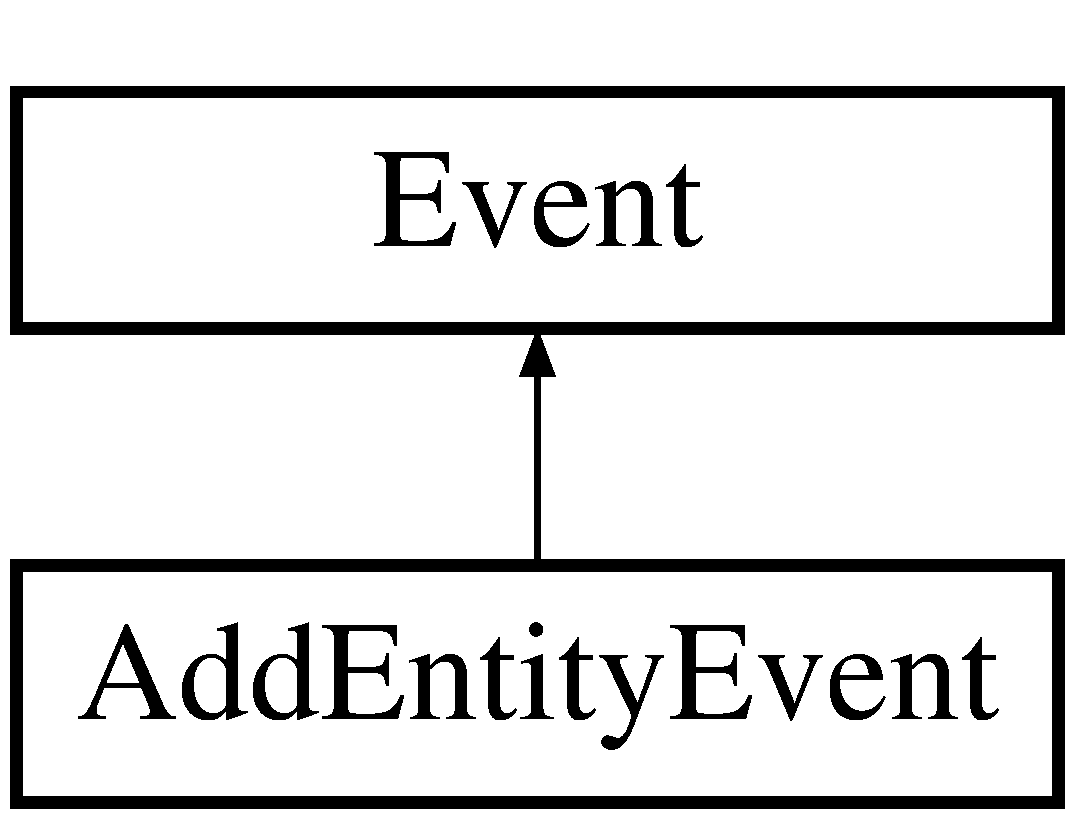
\includegraphics[height=2.000000cm]{classAddEntityEvent}
\end{center}
\end{figure}
\subsection*{Public Member Functions}
\begin{DoxyCompactItemize}
\item 
\hyperlink{classAddEntityEvent_aa173c0bf3732483470f73beb61461eb9}{Add\-Entity\-Event} ()
\item 
\hyperlink{event_8h_a2628ea8d12e8b2563c32f05dc7fff6fa}{Event\-Type} \hyperlink{classEvent_ab0c2e30730d5859851f3126258c0126e}{get\-Type} () const 
\end{DoxyCompactItemize}
\subsection*{Public Attributes}
\begin{DoxyCompactItemize}
\item 
\hyperlink{classEntity}{Entity} $\ast$ \hyperlink{classAddEntityEvent_a2c6f03064f943f33a2db0bf1438b0f93}{entity}
\end{DoxyCompactItemize}
\subsection*{Protected Attributes}
\begin{DoxyCompactItemize}
\item 
\hyperlink{event_8h_a2628ea8d12e8b2563c32f05dc7fff6fa}{Event\-Type} \hyperlink{classEvent_a38264e3fb229dc64123dff1d5a7dcf9e}{m\-\_\-type}
\end{DoxyCompactItemize}


\subsection{Constructor \& Destructor Documentation}
\hypertarget{classAddEntityEvent_aa173c0bf3732483470f73beb61461eb9}{\index{Add\-Entity\-Event@{Add\-Entity\-Event}!Add\-Entity\-Event@{Add\-Entity\-Event}}
\index{Add\-Entity\-Event@{Add\-Entity\-Event}!AddEntityEvent@{Add\-Entity\-Event}}
\subsubsection[{Add\-Entity\-Event}]{\setlength{\rightskip}{0pt plus 5cm}Add\-Entity\-Event\-::\-Add\-Entity\-Event (
\begin{DoxyParamCaption}
{}
\end{DoxyParamCaption}
)\hspace{0.3cm}{\ttfamily [inline]}}}\label{classAddEntityEvent_aa173c0bf3732483470f73beb61461eb9}


\subsection{Member Function Documentation}
\hypertarget{classEvent_ab0c2e30730d5859851f3126258c0126e}{\index{Add\-Entity\-Event@{Add\-Entity\-Event}!get\-Type@{get\-Type}}
\index{get\-Type@{get\-Type}!AddEntityEvent@{Add\-Entity\-Event}}
\subsubsection[{get\-Type}]{\setlength{\rightskip}{0pt plus 5cm}{\bf Event\-Type} Event\-::get\-Type (
\begin{DoxyParamCaption}
{}
\end{DoxyParamCaption}
) const\hspace{0.3cm}{\ttfamily [inline]}, {\ttfamily [inherited]}}}\label{classEvent_ab0c2e30730d5859851f3126258c0126e}


\subsection{Member Data Documentation}
\hypertarget{classAddEntityEvent_a2c6f03064f943f33a2db0bf1438b0f93}{\index{Add\-Entity\-Event@{Add\-Entity\-Event}!entity@{entity}}
\index{entity@{entity}!AddEntityEvent@{Add\-Entity\-Event}}
\subsubsection[{entity}]{\setlength{\rightskip}{0pt plus 5cm}{\bf Entity}$\ast$ Add\-Entity\-Event\-::entity}}\label{classAddEntityEvent_a2c6f03064f943f33a2db0bf1438b0f93}
\hypertarget{classEvent_a38264e3fb229dc64123dff1d5a7dcf9e}{\index{Add\-Entity\-Event@{Add\-Entity\-Event}!m\-\_\-type@{m\-\_\-type}}
\index{m\-\_\-type@{m\-\_\-type}!AddEntityEvent@{Add\-Entity\-Event}}
\subsubsection[{m\-\_\-type}]{\setlength{\rightskip}{0pt plus 5cm}{\bf Event\-Type} Event\-::m\-\_\-type\hspace{0.3cm}{\ttfamily [protected]}, {\ttfamily [inherited]}}}\label{classEvent_a38264e3fb229dc64123dff1d5a7dcf9e}


The documentation for this class was generated from the following file\-:\begin{DoxyCompactItemize}
\item 
\hyperlink{event_8h}{event.\-h}\end{DoxyCompactItemize}

\hypertarget{classAttackEntityEvent}{\section{Attack\-Entity\-Event Class Reference}
\label{classAttackEntityEvent}\index{Attack\-Entity\-Event@{Attack\-Entity\-Event}}
}


{\ttfamily \#include $<$event.\-h$>$}

Inheritance diagram for Attack\-Entity\-Event\-:\begin{figure}[H]
\begin{center}
\leavevmode
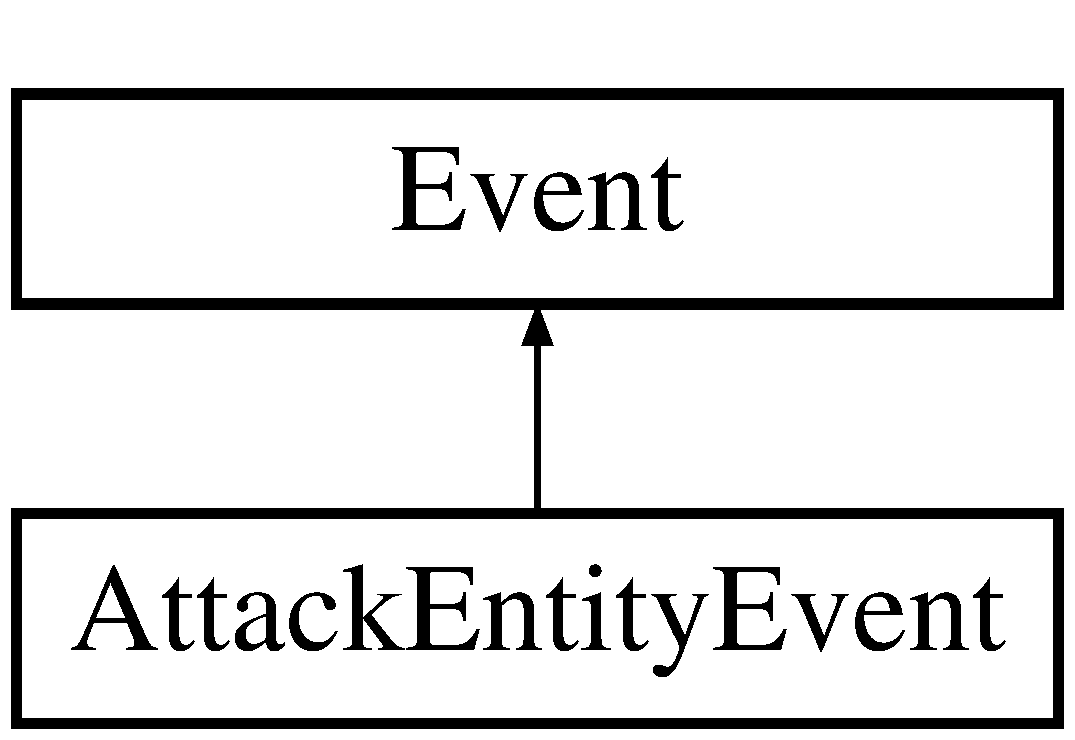
\includegraphics[height=2.000000cm]{classAttackEntityEvent}
\end{center}
\end{figure}
\subsection*{Public Member Functions}
\begin{DoxyCompactItemize}
\item 
\hyperlink{classAttackEntityEvent_a32db1508238dc3f01f18c07531804757}{Attack\-Entity\-Event} ()
\item 
\hyperlink{event_8h_a2628ea8d12e8b2563c32f05dc7fff6fa}{Event\-Type} \hyperlink{classEvent_ab0c2e30730d5859851f3126258c0126e}{get\-Type} () const 
\end{DoxyCompactItemize}
\subsection*{Public Attributes}
\begin{DoxyCompactItemize}
\item 
\hyperlink{classEntity}{Entity} \hyperlink{classAttackEntityEvent_a1dae8f2e2e9224c2bf5f19b665d06a8b}{entity}
\end{DoxyCompactItemize}
\subsection*{Protected Attributes}
\begin{DoxyCompactItemize}
\item 
\hyperlink{event_8h_a2628ea8d12e8b2563c32f05dc7fff6fa}{Event\-Type} \hyperlink{classEvent_a38264e3fb229dc64123dff1d5a7dcf9e}{m\-\_\-type}
\end{DoxyCompactItemize}


\subsection{Constructor \& Destructor Documentation}
\hypertarget{classAttackEntityEvent_a32db1508238dc3f01f18c07531804757}{\index{Attack\-Entity\-Event@{Attack\-Entity\-Event}!Attack\-Entity\-Event@{Attack\-Entity\-Event}}
\index{Attack\-Entity\-Event@{Attack\-Entity\-Event}!AttackEntityEvent@{Attack\-Entity\-Event}}
\subsubsection[{Attack\-Entity\-Event}]{\setlength{\rightskip}{0pt plus 5cm}Attack\-Entity\-Event\-::\-Attack\-Entity\-Event (
\begin{DoxyParamCaption}
{}
\end{DoxyParamCaption}
)\hspace{0.3cm}{\ttfamily [inline]}}}\label{classAttackEntityEvent_a32db1508238dc3f01f18c07531804757}


\subsection{Member Function Documentation}
\hypertarget{classEvent_ab0c2e30730d5859851f3126258c0126e}{\index{Attack\-Entity\-Event@{Attack\-Entity\-Event}!get\-Type@{get\-Type}}
\index{get\-Type@{get\-Type}!AttackEntityEvent@{Attack\-Entity\-Event}}
\subsubsection[{get\-Type}]{\setlength{\rightskip}{0pt plus 5cm}{\bf Event\-Type} Event\-::get\-Type (
\begin{DoxyParamCaption}
{}
\end{DoxyParamCaption}
) const\hspace{0.3cm}{\ttfamily [inline]}, {\ttfamily [inherited]}}}\label{classEvent_ab0c2e30730d5859851f3126258c0126e}


\subsection{Member Data Documentation}
\hypertarget{classAttackEntityEvent_a1dae8f2e2e9224c2bf5f19b665d06a8b}{\index{Attack\-Entity\-Event@{Attack\-Entity\-Event}!entity@{entity}}
\index{entity@{entity}!AttackEntityEvent@{Attack\-Entity\-Event}}
\subsubsection[{entity}]{\setlength{\rightskip}{0pt plus 5cm}{\bf Entity} Attack\-Entity\-Event\-::entity}}\label{classAttackEntityEvent_a1dae8f2e2e9224c2bf5f19b665d06a8b}
\hypertarget{classEvent_a38264e3fb229dc64123dff1d5a7dcf9e}{\index{Attack\-Entity\-Event@{Attack\-Entity\-Event}!m\-\_\-type@{m\-\_\-type}}
\index{m\-\_\-type@{m\-\_\-type}!AttackEntityEvent@{Attack\-Entity\-Event}}
\subsubsection[{m\-\_\-type}]{\setlength{\rightskip}{0pt plus 5cm}{\bf Event\-Type} Event\-::m\-\_\-type\hspace{0.3cm}{\ttfamily [protected]}, {\ttfamily [inherited]}}}\label{classEvent_a38264e3fb229dc64123dff1d5a7dcf9e}


The documentation for this class was generated from the following file\-:\begin{DoxyCompactItemize}
\item 
\hyperlink{event_8h}{event.\-h}\end{DoxyCompactItemize}

\hypertarget{structColliderComponent}{\section{Collider\-Component Struct Reference}
\label{structColliderComponent}\index{Collider\-Component@{Collider\-Component}}
}


{\ttfamily \#include $<$collider\-\_\-component.\-h$>$}



The documentation for this struct was generated from the following file\-:\begin{DoxyCompactItemize}
\item 
\hyperlink{collider__component_8h}{collider\-\_\-component.\-h}\end{DoxyCompactItemize}

\hypertarget{classColor}{\section{Color Class Reference}
\label{classColor}\index{Color@{Color}}
}


{\ttfamily \#include $<$color.\-h$>$}

\subsection*{Public Member Functions}
\begin{DoxyCompactItemize}
\item 
\hyperlink{classColor_a9a742cbe9f9f4037f5d9f4e81a9b2428}{Color} ()
\item 
\hyperlink{classColor_aa347facf3fa618a4817f94bef0c5d424}{Color} (float red, float green, float blue)
\item 
\hyperlink{classColor_a0a169e5ff7cc17872c3f21d652b02497}{Color} (\hyperlink{color_8h_af90824509586333cf45ce757d2711ce3}{C\-O\-L\-O\-R} color)
\item 
float \hyperlink{classColor_ae212502d1420f4b935dad02b9b17131a}{Red} ()
\item 
float \hyperlink{classColor_a6fac5c8fc1822b01d2f5500ba906eb6e}{Green} ()
\item 
float \hyperlink{classColor_a9bba5de22a953eb924173eb1c207f667}{Blue} ()
\end{DoxyCompactItemize}
\subsection*{Private Attributes}
\begin{DoxyCompactItemize}
\item 
float \hyperlink{classColor_a6da1cc1b1358e18dce5fc0335a8abdb6}{m\-\_\-red}
\item 
float \hyperlink{classColor_a6c884c0a93f4e23c5db71d003ec2857a}{m\-\_\-green}
\item 
float \hyperlink{classColor_a68e36f358a0d335e9a7cadd748cb67b5}{m\-\_\-blue}
\end{DoxyCompactItemize}


\subsection{Constructor \& Destructor Documentation}
\hypertarget{classColor_a9a742cbe9f9f4037f5d9f4e81a9b2428}{\index{Color@{Color}!Color@{Color}}
\index{Color@{Color}!Color@{Color}}
\subsubsection[{Color}]{\setlength{\rightskip}{0pt plus 5cm}Color\-::\-Color (
\begin{DoxyParamCaption}
{}
\end{DoxyParamCaption}
)\hspace{0.3cm}{\ttfamily [inline]}}}\label{classColor_a9a742cbe9f9f4037f5d9f4e81a9b2428}
\hypertarget{classColor_aa347facf3fa618a4817f94bef0c5d424}{\index{Color@{Color}!Color@{Color}}
\index{Color@{Color}!Color@{Color}}
\subsubsection[{Color}]{\setlength{\rightskip}{0pt plus 5cm}Color\-::\-Color (
\begin{DoxyParamCaption}
\item[{float}]{red, }
\item[{float}]{green, }
\item[{float}]{blue}
\end{DoxyParamCaption}
)}}\label{classColor_aa347facf3fa618a4817f94bef0c5d424}
\hypertarget{classColor_a0a169e5ff7cc17872c3f21d652b02497}{\index{Color@{Color}!Color@{Color}}
\index{Color@{Color}!Color@{Color}}
\subsubsection[{Color}]{\setlength{\rightskip}{0pt plus 5cm}Color\-::\-Color (
\begin{DoxyParamCaption}
\item[{{\bf C\-O\-L\-O\-R}}]{color}
\end{DoxyParamCaption}
)}}\label{classColor_a0a169e5ff7cc17872c3f21d652b02497}


\subsection{Member Function Documentation}
\hypertarget{classColor_a9bba5de22a953eb924173eb1c207f667}{\index{Color@{Color}!Blue@{Blue}}
\index{Blue@{Blue}!Color@{Color}}
\subsubsection[{Blue}]{\setlength{\rightskip}{0pt plus 5cm}float Color\-::\-Blue (
\begin{DoxyParamCaption}
{}
\end{DoxyParamCaption}
)\hspace{0.3cm}{\ttfamily [inline]}}}\label{classColor_a9bba5de22a953eb924173eb1c207f667}
\hypertarget{classColor_a6fac5c8fc1822b01d2f5500ba906eb6e}{\index{Color@{Color}!Green@{Green}}
\index{Green@{Green}!Color@{Color}}
\subsubsection[{Green}]{\setlength{\rightskip}{0pt plus 5cm}float Color\-::\-Green (
\begin{DoxyParamCaption}
{}
\end{DoxyParamCaption}
)\hspace{0.3cm}{\ttfamily [inline]}}}\label{classColor_a6fac5c8fc1822b01d2f5500ba906eb6e}
\hypertarget{classColor_ae212502d1420f4b935dad02b9b17131a}{\index{Color@{Color}!Red@{Red}}
\index{Red@{Red}!Color@{Color}}
\subsubsection[{Red}]{\setlength{\rightskip}{0pt plus 5cm}float Color\-::\-Red (
\begin{DoxyParamCaption}
{}
\end{DoxyParamCaption}
)\hspace{0.3cm}{\ttfamily [inline]}}}\label{classColor_ae212502d1420f4b935dad02b9b17131a}


\subsection{Member Data Documentation}
\hypertarget{classColor_a68e36f358a0d335e9a7cadd748cb67b5}{\index{Color@{Color}!m\-\_\-blue@{m\-\_\-blue}}
\index{m\-\_\-blue@{m\-\_\-blue}!Color@{Color}}
\subsubsection[{m\-\_\-blue}]{\setlength{\rightskip}{0pt plus 5cm}float Color\-::m\-\_\-blue\hspace{0.3cm}{\ttfamily [private]}}}\label{classColor_a68e36f358a0d335e9a7cadd748cb67b5}
\hypertarget{classColor_a6c884c0a93f4e23c5db71d003ec2857a}{\index{Color@{Color}!m\-\_\-green@{m\-\_\-green}}
\index{m\-\_\-green@{m\-\_\-green}!Color@{Color}}
\subsubsection[{m\-\_\-green}]{\setlength{\rightskip}{0pt plus 5cm}float Color\-::m\-\_\-green\hspace{0.3cm}{\ttfamily [private]}}}\label{classColor_a6c884c0a93f4e23c5db71d003ec2857a}
\hypertarget{classColor_a6da1cc1b1358e18dce5fc0335a8abdb6}{\index{Color@{Color}!m\-\_\-red@{m\-\_\-red}}
\index{m\-\_\-red@{m\-\_\-red}!Color@{Color}}
\subsubsection[{m\-\_\-red}]{\setlength{\rightskip}{0pt plus 5cm}float Color\-::m\-\_\-red\hspace{0.3cm}{\ttfamily [private]}}}\label{classColor_a6da1cc1b1358e18dce5fc0335a8abdb6}


The documentation for this class was generated from the following files\-:\begin{DoxyCompactItemize}
\item 
\hyperlink{color_8h}{color.\-h}\item 
\hyperlink{color_8cpp}{color.\-cpp}\end{DoxyCompactItemize}

\hypertarget{classCombatSystem}{\section{Combat\-System Class Reference}
\label{classCombatSystem}\index{Combat\-System@{Combat\-System}}
}


{\ttfamily \#include $<$combat\-\_\-system.\-h$>$}

Inheritance diagram for Combat\-System\-:\begin{figure}[H]
\begin{center}
\leavevmode
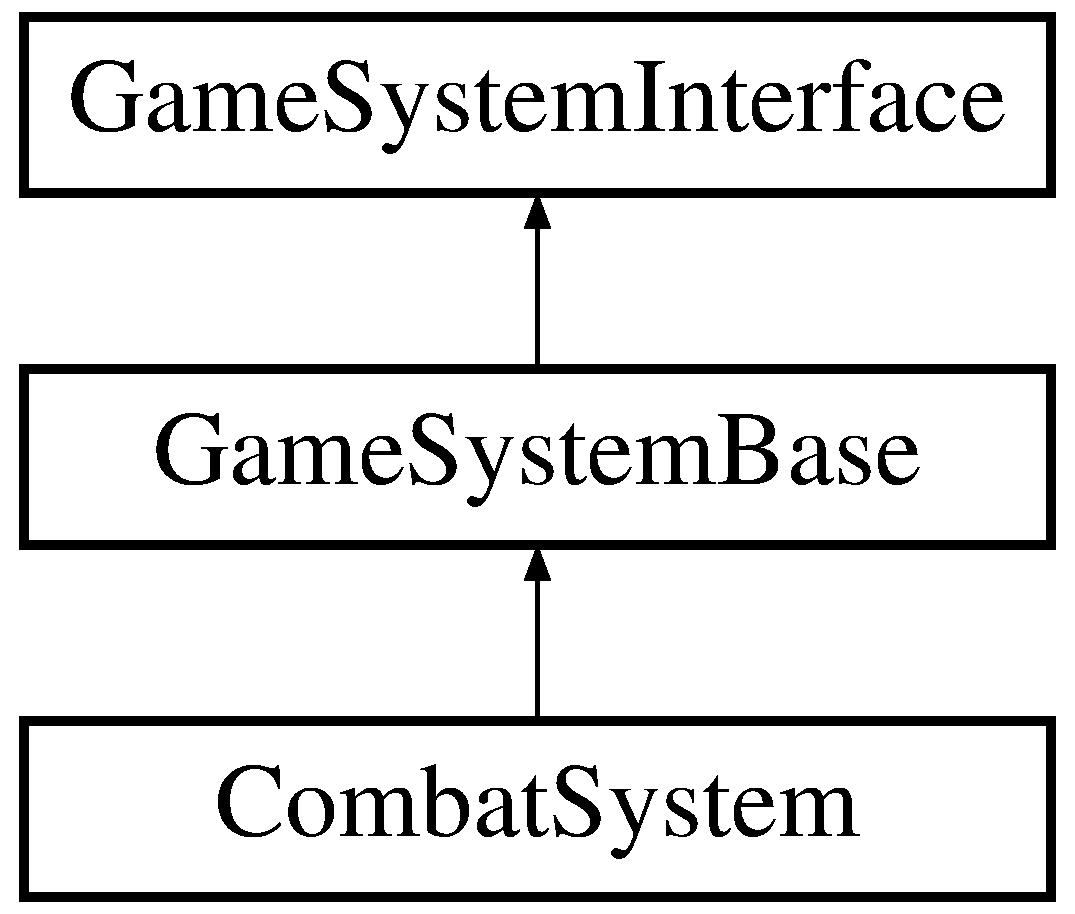
\includegraphics[height=3.000000cm]{classCombatSystem}
\end{center}
\end{figure}
\subsection*{Public Member Functions}
\begin{DoxyCompactItemize}
\item 
virtual void \hyperlink{classCombatSystem_afba5db4bb69a947c3a2303005f74d5d7}{handle\-Event} (const \hyperlink{classEvent}{Event} $\ast$event)
\item 
virtual void \hyperlink{classGameSystemBase_a55b4fc27cbfccd3c724c2e5984d78625}{initialise} (\hyperlink{classGameEngineInterface}{Game\-Engine\-Interface} $\ast$engine)
\item 
virtual \hyperlink{classGameEngineInterface}{Game\-Engine\-Interface} $\ast$ \hyperlink{classGameSystemBase_a1954c5a1c79963554805bc25b2cd6072}{get\-Engine\-Ref} ()
\item 
virtual void \hyperlink{classGameSystemBase_a039d3086ac7fe50abdb110b569520d69}{update} ()
\item 
virtual std\-::vector$<$ \hyperlink{classEntity}{Entity} $\ast$ $>$ \hyperlink{classGameSystemBase_aae270a88f1077a091e6033514b889abd}{find\-Entities\-Near} (unsigned int x, unsigned int y, unsigned radius)
\item 
virtual std\-::vector$<$ \hyperlink{classEntity}{Entity} $\ast$ $>$ \hyperlink{classGameSystemBase_a7aa9912fc078d990dbfb480e411bd3bc}{find\-Entities\-At} (unsigned int x, unsigned int y)
\item 
virtual std\-::vector$<$ \hyperlink{classEntity}{Entity} $\ast$ $>$ \hyperlink{classGameSystemBase_a44456ef40ac565b9d6b65f3b1531a4ef}{find\-Entities\-To\-The} (\hyperlink{classMoveEntityEvent_a7058a943643bee9164a21e62e3392807}{Move\-Entity\-Event\-::\-D\-I\-R\-E\-C\-T\-I\-O\-N} a\-\_\-direction, \hyperlink{classEntity}{Entity} $\ast$a\-\_\-entity)
\end{DoxyCompactItemize}
\subsection*{Protected Attributes}
\begin{DoxyCompactItemize}
\item 
\hyperlink{classGameEngineInterface}{Game\-Engine\-Interface} $\ast$ \hyperlink{classGameSystemBase_aa9044eb22399f0c0ddd8f049738c62e5}{m\-\_\-engine}
\end{DoxyCompactItemize}
\subsection*{Private Member Functions}
\begin{DoxyCompactItemize}
\item 
bool \hyperlink{classCombatSystem_aa60d601edd993b6a7bded45d0e786595}{check\-For\-Enemies} (\hyperlink{classMoveEntityEvent_a7058a943643bee9164a21e62e3392807}{Move\-Entity\-Event\-::\-D\-I\-R\-E\-C\-T\-I\-O\-N} dir)
\end{DoxyCompactItemize}


\subsection{Member Function Documentation}
\hypertarget{classCombatSystem_aa60d601edd993b6a7bded45d0e786595}{\index{Combat\-System@{Combat\-System}!check\-For\-Enemies@{check\-For\-Enemies}}
\index{check\-For\-Enemies@{check\-For\-Enemies}!CombatSystem@{Combat\-System}}
\subsubsection[{check\-For\-Enemies}]{\setlength{\rightskip}{0pt plus 5cm}bool Combat\-System\-::check\-For\-Enemies (
\begin{DoxyParamCaption}
\item[{{\bf Move\-Entity\-Event\-::\-D\-I\-R\-E\-C\-T\-I\-O\-N}}]{dir}
\end{DoxyParamCaption}
)\hspace{0.3cm}{\ttfamily [private]}}}\label{classCombatSystem_aa60d601edd993b6a7bded45d0e786595}
\hypertarget{classGameSystemBase_a7aa9912fc078d990dbfb480e411bd3bc}{\index{Combat\-System@{Combat\-System}!find\-Entities\-At@{find\-Entities\-At}}
\index{find\-Entities\-At@{find\-Entities\-At}!CombatSystem@{Combat\-System}}
\subsubsection[{find\-Entities\-At}]{\setlength{\rightskip}{0pt plus 5cm}std\-::vector$<$ {\bf Entity} $\ast$ $>$ Game\-System\-Base\-::find\-Entities\-At (
\begin{DoxyParamCaption}
\item[{unsigned int}]{x, }
\item[{unsigned int}]{y}
\end{DoxyParamCaption}
)\hspace{0.3cm}{\ttfamily [virtual]}, {\ttfamily [inherited]}}}\label{classGameSystemBase_a7aa9912fc078d990dbfb480e411bd3bc}
\hypertarget{classGameSystemBase_aae270a88f1077a091e6033514b889abd}{\index{Combat\-System@{Combat\-System}!find\-Entities\-Near@{find\-Entities\-Near}}
\index{find\-Entities\-Near@{find\-Entities\-Near}!CombatSystem@{Combat\-System}}
\subsubsection[{find\-Entities\-Near}]{\setlength{\rightskip}{0pt plus 5cm}std\-::vector$<$ {\bf Entity} $\ast$ $>$ Game\-System\-Base\-::find\-Entities\-Near (
\begin{DoxyParamCaption}
\item[{unsigned int}]{x, }
\item[{unsigned int}]{y, }
\item[{unsigned}]{radius}
\end{DoxyParamCaption}
)\hspace{0.3cm}{\ttfamily [virtual]}, {\ttfamily [inherited]}}}\label{classGameSystemBase_aae270a88f1077a091e6033514b889abd}
\hypertarget{classGameSystemBase_a44456ef40ac565b9d6b65f3b1531a4ef}{\index{Combat\-System@{Combat\-System}!find\-Entities\-To\-The@{find\-Entities\-To\-The}}
\index{find\-Entities\-To\-The@{find\-Entities\-To\-The}!CombatSystem@{Combat\-System}}
\subsubsection[{find\-Entities\-To\-The}]{\setlength{\rightskip}{0pt plus 5cm}std\-::vector$<$ {\bf Entity} $\ast$ $>$ Game\-System\-Base\-::find\-Entities\-To\-The (
\begin{DoxyParamCaption}
\item[{{\bf Move\-Entity\-Event\-::\-D\-I\-R\-E\-C\-T\-I\-O\-N}}]{a\-\_\-direction, }
\item[{{\bf Entity} $\ast$}]{a\-\_\-entity}
\end{DoxyParamCaption}
)\hspace{0.3cm}{\ttfamily [virtual]}, {\ttfamily [inherited]}}}\label{classGameSystemBase_a44456ef40ac565b9d6b65f3b1531a4ef}
\hypertarget{classGameSystemBase_a1954c5a1c79963554805bc25b2cd6072}{\index{Combat\-System@{Combat\-System}!get\-Engine\-Ref@{get\-Engine\-Ref}}
\index{get\-Engine\-Ref@{get\-Engine\-Ref}!CombatSystem@{Combat\-System}}
\subsubsection[{get\-Engine\-Ref}]{\setlength{\rightskip}{0pt plus 5cm}virtual {\bf Game\-Engine\-Interface}$\ast$ Game\-System\-Base\-::get\-Engine\-Ref (
\begin{DoxyParamCaption}
{}
\end{DoxyParamCaption}
)\hspace{0.3cm}{\ttfamily [inline]}, {\ttfamily [virtual]}, {\ttfamily [inherited]}}}\label{classGameSystemBase_a1954c5a1c79963554805bc25b2cd6072}
\hypertarget{classCombatSystem_afba5db4bb69a947c3a2303005f74d5d7}{\index{Combat\-System@{Combat\-System}!handle\-Event@{handle\-Event}}
\index{handle\-Event@{handle\-Event}!CombatSystem@{Combat\-System}}
\subsubsection[{handle\-Event}]{\setlength{\rightskip}{0pt plus 5cm}void Combat\-System\-::handle\-Event (
\begin{DoxyParamCaption}
\item[{const {\bf Event} $\ast$}]{event}
\end{DoxyParamCaption}
)\hspace{0.3cm}{\ttfamily [virtual]}}}\label{classCombatSystem_afba5db4bb69a947c3a2303005f74d5d7}


Reimplemented from \hyperlink{classGameSystemBase_a007b3ece290b1ad0dc3e397c5264d44d}{Game\-System\-Base}.

\hypertarget{classGameSystemBase_a55b4fc27cbfccd3c724c2e5984d78625}{\index{Combat\-System@{Combat\-System}!initialise@{initialise}}
\index{initialise@{initialise}!CombatSystem@{Combat\-System}}
\subsubsection[{initialise}]{\setlength{\rightskip}{0pt plus 5cm}virtual void Game\-System\-Base\-::initialise (
\begin{DoxyParamCaption}
\item[{{\bf Game\-Engine\-Interface} $\ast$}]{engine}
\end{DoxyParamCaption}
)\hspace{0.3cm}{\ttfamily [inline]}, {\ttfamily [virtual]}, {\ttfamily [inherited]}}}\label{classGameSystemBase_a55b4fc27cbfccd3c724c2e5984d78625}


Implements \hyperlink{classGameSystemInterface_a29079ef1f35027150b751c3fcb025091}{Game\-System\-Interface}.

\hypertarget{classGameSystemBase_a039d3086ac7fe50abdb110b569520d69}{\index{Combat\-System@{Combat\-System}!update@{update}}
\index{update@{update}!CombatSystem@{Combat\-System}}
\subsubsection[{update}]{\setlength{\rightskip}{0pt plus 5cm}virtual void Game\-System\-Base\-::update (
\begin{DoxyParamCaption}
{}
\end{DoxyParamCaption}
)\hspace{0.3cm}{\ttfamily [inline]}, {\ttfamily [virtual]}, {\ttfamily [inherited]}}}\label{classGameSystemBase_a039d3086ac7fe50abdb110b569520d69}


Implements \hyperlink{classGameSystemInterface_a531f5e7c6ca9881a67932cc4fded0a2e}{Game\-System\-Interface}.



Reimplemented in \hyperlink{classNpcSystem_a88d87a8ec981e5cf1f4ed4340123a9d8}{Npc\-System}.



\subsection{Member Data Documentation}
\hypertarget{classGameSystemBase_aa9044eb22399f0c0ddd8f049738c62e5}{\index{Combat\-System@{Combat\-System}!m\-\_\-engine@{m\-\_\-engine}}
\index{m\-\_\-engine@{m\-\_\-engine}!CombatSystem@{Combat\-System}}
\subsubsection[{m\-\_\-engine}]{\setlength{\rightskip}{0pt plus 5cm}{\bf Game\-Engine\-Interface}$\ast$ Game\-System\-Base\-::m\-\_\-engine\hspace{0.3cm}{\ttfamily [protected]}, {\ttfamily [inherited]}}}\label{classGameSystemBase_aa9044eb22399f0c0ddd8f049738c62e5}


The documentation for this class was generated from the following files\-:\begin{DoxyCompactItemize}
\item 
\hyperlink{combat__system_8h}{combat\-\_\-system.\-h}\item 
\hyperlink{combat__system_8cpp}{combat\-\_\-system.\-cpp}\end{DoxyCompactItemize}

\hypertarget{classComponentManager}{\section{Component\-Manager$<$ T $>$ Class Template Reference}
\label{classComponentManager}\index{Component\-Manager$<$ T $>$@{Component\-Manager$<$ T $>$}}
}


{\ttfamily \#include $<$component\-\_\-manager.\-h$>$}

Inheritance diagram for Component\-Manager$<$ T $>$\-:\begin{figure}[H]
\begin{center}
\leavevmode
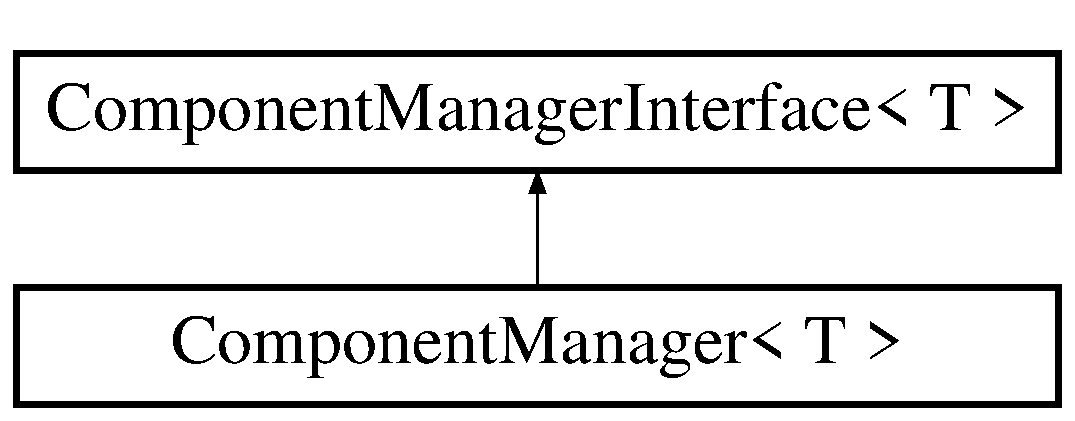
\includegraphics[height=2.000000cm]{classComponentManager}
\end{center}
\end{figure}
\subsection*{Public Member Functions}
\begin{DoxyCompactItemize}
\item 
void \hyperlink{classComponentManager_a47a5b1a0e0dcc81b602f2cce15ef26c1}{add} (\hyperlink{classEntity}{Entity} $\ast$entity, T component)
\item 
T $\ast$ \hyperlink{classComponentManager_ae0cecdacbc85227b566fd45620201d29}{get} (\hyperlink{classEntity}{Entity} $\ast$entity)
\item 
void \hyperlink{classComponentManager_aaed6a884b2e6be899d61858e35983bd8}{remove} (\hyperlink{classEntity}{Entity} $\ast$entity)
\item 
std\-::map$<$ \hyperlink{classEntity}{Entity} $\ast$, T $>$ \& \hyperlink{classComponentManager_afd23cc5da5ff3be1e4173fff6d5fddf4}{get\-All} ()
\end{DoxyCompactItemize}
\subsection*{Private Attributes}
\begin{DoxyCompactItemize}
\item 
std\-::map$<$ \hyperlink{classEntity}{Entity} $\ast$, T $>$ \hyperlink{classComponentManager_a807cc91da58969a861dca5fb604bd1b5}{m\-\_\-components}
\end{DoxyCompactItemize}


\subsection{Member Function Documentation}
\hypertarget{classComponentManager_a47a5b1a0e0dcc81b602f2cce15ef26c1}{\index{Component\-Manager@{Component\-Manager}!add@{add}}
\index{add@{add}!ComponentManager@{Component\-Manager}}
\subsubsection[{add}]{\setlength{\rightskip}{0pt plus 5cm}template$<$class T$>$ void {\bf Component\-Manager}$<$ T $>$\-::add (
\begin{DoxyParamCaption}
\item[{{\bf Entity} $\ast$}]{entity, }
\item[{T}]{component}
\end{DoxyParamCaption}
)\hspace{0.3cm}{\ttfamily [virtual]}}}\label{classComponentManager_a47a5b1a0e0dcc81b602f2cce15ef26c1}


Implements \hyperlink{classComponentManagerInterface_a6eb928ae754e61c5cb65ac279706ba29}{Component\-Manager\-Interface$<$ T $>$}.

\hypertarget{classComponentManager_ae0cecdacbc85227b566fd45620201d29}{\index{Component\-Manager@{Component\-Manager}!get@{get}}
\index{get@{get}!ComponentManager@{Component\-Manager}}
\subsubsection[{get}]{\setlength{\rightskip}{0pt plus 5cm}template$<$class T $>$ T $\ast$ {\bf Component\-Manager}$<$ T $>$\-::get (
\begin{DoxyParamCaption}
\item[{{\bf Entity} $\ast$}]{entity}
\end{DoxyParamCaption}
)\hspace{0.3cm}{\ttfamily [virtual]}}}\label{classComponentManager_ae0cecdacbc85227b566fd45620201d29}


Implements \hyperlink{classComponentManagerInterface_aa56b700c4ea98e708c68ebbde3205fd9}{Component\-Manager\-Interface$<$ T $>$}.

\hypertarget{classComponentManager_afd23cc5da5ff3be1e4173fff6d5fddf4}{\index{Component\-Manager@{Component\-Manager}!get\-All@{get\-All}}
\index{get\-All@{get\-All}!ComponentManager@{Component\-Manager}}
\subsubsection[{get\-All}]{\setlength{\rightskip}{0pt plus 5cm}template$<$class T$>$ std\-::map$<${\bf Entity}$\ast$, T$>$\& {\bf Component\-Manager}$<$ T $>$\-::get\-All (
\begin{DoxyParamCaption}
{}
\end{DoxyParamCaption}
)\hspace{0.3cm}{\ttfamily [inline]}, {\ttfamily [virtual]}}}\label{classComponentManager_afd23cc5da5ff3be1e4173fff6d5fddf4}


Implements \hyperlink{classComponentManagerInterface_a2ea45742be30438171b9b24fb36a5761}{Component\-Manager\-Interface$<$ T $>$}.

\hypertarget{classComponentManager_aaed6a884b2e6be899d61858e35983bd8}{\index{Component\-Manager@{Component\-Manager}!remove@{remove}}
\index{remove@{remove}!ComponentManager@{Component\-Manager}}
\subsubsection[{remove}]{\setlength{\rightskip}{0pt plus 5cm}template$<$class T $>$ void {\bf Component\-Manager}$<$ T $>$\-::remove (
\begin{DoxyParamCaption}
\item[{{\bf Entity} $\ast$}]{entity}
\end{DoxyParamCaption}
)\hspace{0.3cm}{\ttfamily [virtual]}}}\label{classComponentManager_aaed6a884b2e6be899d61858e35983bd8}


Implements \hyperlink{classComponentManagerInterface_a3ef2198d5c9661418bff0c9f194cb2ce}{Component\-Manager\-Interface$<$ T $>$}.



\subsection{Member Data Documentation}
\hypertarget{classComponentManager_a807cc91da58969a861dca5fb604bd1b5}{\index{Component\-Manager@{Component\-Manager}!m\-\_\-components@{m\-\_\-components}}
\index{m\-\_\-components@{m\-\_\-components}!ComponentManager@{Component\-Manager}}
\subsubsection[{m\-\_\-components}]{\setlength{\rightskip}{0pt plus 5cm}template$<$class T$>$ std\-::map$<${\bf Entity}$\ast$, T$>$ {\bf Component\-Manager}$<$ T $>$\-::m\-\_\-components\hspace{0.3cm}{\ttfamily [private]}}}\label{classComponentManager_a807cc91da58969a861dca5fb604bd1b5}


The documentation for this class was generated from the following file\-:\begin{DoxyCompactItemize}
\item 
\hyperlink{component__manager_8h}{component\-\_\-manager.\-h}\end{DoxyCompactItemize}

\hypertarget{classComponentManagerInterface}{\section{Component\-Manager\-Interface$<$ T $>$ Class Template Reference}
\label{classComponentManagerInterface}\index{Component\-Manager\-Interface$<$ T $>$@{Component\-Manager\-Interface$<$ T $>$}}
}


{\ttfamily \#include $<$component\-\_\-manager\-\_\-interface.\-h$>$}

Inheritance diagram for Component\-Manager\-Interface$<$ T $>$\-:\begin{figure}[H]
\begin{center}
\leavevmode
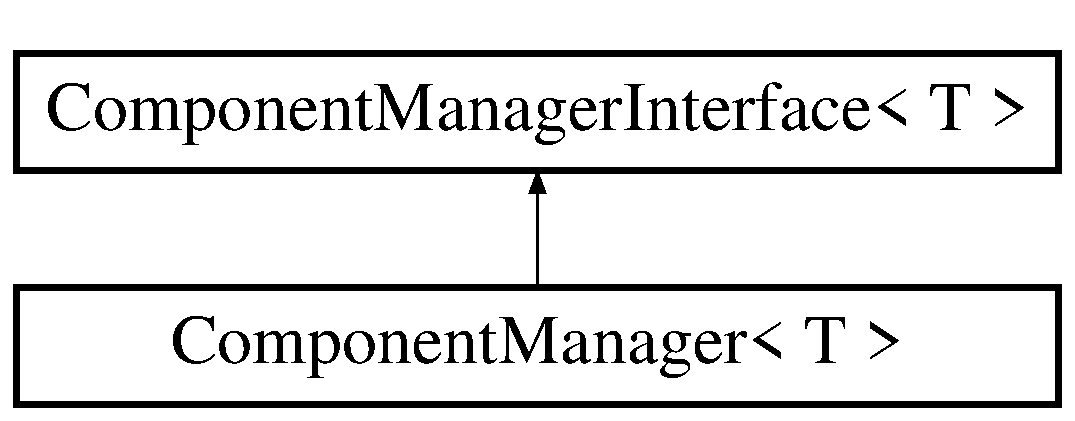
\includegraphics[height=2.000000cm]{classComponentManagerInterface}
\end{center}
\end{figure}
\subsection*{Public Member Functions}
\begin{DoxyCompactItemize}
\item 
virtual \hyperlink{classComponentManagerInterface_a4693483e5744014f340619627e0ee31b}{$\sim$\-Component\-Manager\-Interface} ()
\item 
virtual void \hyperlink{classComponentManagerInterface_a6eb928ae754e61c5cb65ac279706ba29}{add} (\hyperlink{classEntity}{Entity} $\ast$entity, T component)=0
\item 
virtual T $\ast$ \hyperlink{classComponentManagerInterface_aa56b700c4ea98e708c68ebbde3205fd9}{get} (\hyperlink{classEntity}{Entity} $\ast$entity)=0
\item 
virtual void \hyperlink{classComponentManagerInterface_a3ef2198d5c9661418bff0c9f194cb2ce}{remove} (\hyperlink{classEntity}{Entity} $\ast$entity)=0
\item 
virtual std\-::map$<$ \hyperlink{classEntity}{Entity} $\ast$, T $>$ \& \hyperlink{classComponentManagerInterface_a2ea45742be30438171b9b24fb36a5761}{get\-All} ()=0
\end{DoxyCompactItemize}


\subsection{Constructor \& Destructor Documentation}
\hypertarget{classComponentManagerInterface_a4693483e5744014f340619627e0ee31b}{\index{Component\-Manager\-Interface@{Component\-Manager\-Interface}!$\sim$\-Component\-Manager\-Interface@{$\sim$\-Component\-Manager\-Interface}}
\index{$\sim$\-Component\-Manager\-Interface@{$\sim$\-Component\-Manager\-Interface}!ComponentManagerInterface@{Component\-Manager\-Interface}}
\subsubsection[{$\sim$\-Component\-Manager\-Interface}]{\setlength{\rightskip}{0pt plus 5cm}template$<$class T$>$ virtual {\bf Component\-Manager\-Interface}$<$ T $>$\-::$\sim${\bf Component\-Manager\-Interface} (
\begin{DoxyParamCaption}
{}
\end{DoxyParamCaption}
)\hspace{0.3cm}{\ttfamily [inline]}, {\ttfamily [virtual]}}}\label{classComponentManagerInterface_a4693483e5744014f340619627e0ee31b}


\subsection{Member Function Documentation}
\hypertarget{classComponentManagerInterface_a6eb928ae754e61c5cb65ac279706ba29}{\index{Component\-Manager\-Interface@{Component\-Manager\-Interface}!add@{add}}
\index{add@{add}!ComponentManagerInterface@{Component\-Manager\-Interface}}
\subsubsection[{add}]{\setlength{\rightskip}{0pt plus 5cm}template$<$class T$>$ virtual void {\bf Component\-Manager\-Interface}$<$ T $>$\-::add (
\begin{DoxyParamCaption}
\item[{{\bf Entity} $\ast$}]{entity, }
\item[{T}]{component}
\end{DoxyParamCaption}
)\hspace{0.3cm}{\ttfamily [pure virtual]}}}\label{classComponentManagerInterface_a6eb928ae754e61c5cb65ac279706ba29}


Implemented in \hyperlink{classComponentManager_a47a5b1a0e0dcc81b602f2cce15ef26c1}{Component\-Manager$<$ T $>$}, \hyperlink{classComponentManager_a47a5b1a0e0dcc81b602f2cce15ef26c1}{Component\-Manager$<$ Sprite\-Component $>$}, and \hyperlink{classComponentManager_a47a5b1a0e0dcc81b602f2cce15ef26c1}{Component\-Manager$<$ Collider\-Component $>$}.

\hypertarget{classComponentManagerInterface_aa56b700c4ea98e708c68ebbde3205fd9}{\index{Component\-Manager\-Interface@{Component\-Manager\-Interface}!get@{get}}
\index{get@{get}!ComponentManagerInterface@{Component\-Manager\-Interface}}
\subsubsection[{get}]{\setlength{\rightskip}{0pt plus 5cm}template$<$class T$>$ virtual T$\ast$ {\bf Component\-Manager\-Interface}$<$ T $>$\-::get (
\begin{DoxyParamCaption}
\item[{{\bf Entity} $\ast$}]{entity}
\end{DoxyParamCaption}
)\hspace{0.3cm}{\ttfamily [pure virtual]}}}\label{classComponentManagerInterface_aa56b700c4ea98e708c68ebbde3205fd9}


Implemented in \hyperlink{classComponentManager_ae0cecdacbc85227b566fd45620201d29}{Component\-Manager$<$ T $>$}, \hyperlink{classComponentManager_ae0cecdacbc85227b566fd45620201d29}{Component\-Manager$<$ Sprite\-Component $>$}, and \hyperlink{classComponentManager_ae0cecdacbc85227b566fd45620201d29}{Component\-Manager$<$ Collider\-Component $>$}.

\hypertarget{classComponentManagerInterface_a2ea45742be30438171b9b24fb36a5761}{\index{Component\-Manager\-Interface@{Component\-Manager\-Interface}!get\-All@{get\-All}}
\index{get\-All@{get\-All}!ComponentManagerInterface@{Component\-Manager\-Interface}}
\subsubsection[{get\-All}]{\setlength{\rightskip}{0pt plus 5cm}template$<$class T$>$ virtual std\-::map$<${\bf Entity}$\ast$, T$>$\& {\bf Component\-Manager\-Interface}$<$ T $>$\-::get\-All (
\begin{DoxyParamCaption}
{}
\end{DoxyParamCaption}
)\hspace{0.3cm}{\ttfamily [pure virtual]}}}\label{classComponentManagerInterface_a2ea45742be30438171b9b24fb36a5761}


Implemented in \hyperlink{classComponentManager_afd23cc5da5ff3be1e4173fff6d5fddf4}{Component\-Manager$<$ T $>$}, \hyperlink{classComponentManager_afd23cc5da5ff3be1e4173fff6d5fddf4}{Component\-Manager$<$ Sprite\-Component $>$}, and \hyperlink{classComponentManager_afd23cc5da5ff3be1e4173fff6d5fddf4}{Component\-Manager$<$ Collider\-Component $>$}.

\hypertarget{classComponentManagerInterface_a3ef2198d5c9661418bff0c9f194cb2ce}{\index{Component\-Manager\-Interface@{Component\-Manager\-Interface}!remove@{remove}}
\index{remove@{remove}!ComponentManagerInterface@{Component\-Manager\-Interface}}
\subsubsection[{remove}]{\setlength{\rightskip}{0pt plus 5cm}template$<$class T$>$ virtual void {\bf Component\-Manager\-Interface}$<$ T $>$\-::remove (
\begin{DoxyParamCaption}
\item[{{\bf Entity} $\ast$}]{entity}
\end{DoxyParamCaption}
)\hspace{0.3cm}{\ttfamily [pure virtual]}}}\label{classComponentManagerInterface_a3ef2198d5c9661418bff0c9f194cb2ce}


Implemented in \hyperlink{classComponentManager_aaed6a884b2e6be899d61858e35983bd8}{Component\-Manager$<$ T $>$}, \hyperlink{classComponentManager_aaed6a884b2e6be899d61858e35983bd8}{Component\-Manager$<$ Sprite\-Component $>$}, and \hyperlink{classComponentManager_aaed6a884b2e6be899d61858e35983bd8}{Component\-Manager$<$ Collider\-Component $>$}.



The documentation for this class was generated from the following file\-:\begin{DoxyCompactItemize}
\item 
\hyperlink{component__manager__interface_8h}{component\-\_\-manager\-\_\-interface.\-h}\end{DoxyCompactItemize}

\hypertarget{classConfigManager}{\section{Config\-Manager Class Reference}
\label{classConfigManager}\index{Config\-Manager@{Config\-Manager}}
}


{\ttfamily \#include $<$config\-\_\-manager.\-h$>$}

\subsection*{Public Member Functions}
\begin{DoxyCompactItemize}
\item 
void \hyperlink{classConfigManager_a02426e2b6a4bb2c1b2f3c9ef524c772f}{set\-Tag} (const std\-::string \&tag, const \hyperlink{structTagValue}{Tag\-Value} \&val)
\item 
\hyperlink{structTagValue}{Tag\-Value} \hyperlink{classConfigManager_aa43f0b0afd5d15642bb986e17887abdc}{get\-Tag} (const std\-::string \&tag)
\item 
void \hyperlink{classConfigManager_ac50ce34c67bb3157c8504b99d4b705da}{read\-File} (const std\-::string \&config)
\item 
void \hyperlink{classConfigManager_a6aab6b3a9a25bc6341fb18f3b7c569b6}{string\-To\-Tag\-Value} (const std\-::string \&input, \hyperlink{structTagValue}{Tag\-Value} \&output)
\end{DoxyCompactItemize}
\subsection*{Private Attributes}
\begin{DoxyCompactItemize}
\item 
std\-::map$<$ std\-::string, \hyperlink{structTagValue}{Tag\-Value} $>$ \hyperlink{classConfigManager_a5f856d0055899581bd138476045de013}{m\-\_\-tags}
\end{DoxyCompactItemize}


\subsection{Member Function Documentation}
\hypertarget{classConfigManager_aa43f0b0afd5d15642bb986e17887abdc}{\index{Config\-Manager@{Config\-Manager}!get\-Tag@{get\-Tag}}
\index{get\-Tag@{get\-Tag}!ConfigManager@{Config\-Manager}}
\subsubsection[{get\-Tag}]{\setlength{\rightskip}{0pt plus 5cm}{\bf Tag\-Value} Config\-Manager\-::get\-Tag (
\begin{DoxyParamCaption}
\item[{const std\-::string \&}]{tag}
\end{DoxyParamCaption}
)}}\label{classConfigManager_aa43f0b0afd5d15642bb986e17887abdc}
\hypertarget{classConfigManager_ac50ce34c67bb3157c8504b99d4b705da}{\index{Config\-Manager@{Config\-Manager}!read\-File@{read\-File}}
\index{read\-File@{read\-File}!ConfigManager@{Config\-Manager}}
\subsubsection[{read\-File}]{\setlength{\rightskip}{0pt plus 5cm}void Config\-Manager\-::read\-File (
\begin{DoxyParamCaption}
\item[{const std\-::string \&}]{config}
\end{DoxyParamCaption}
)}}\label{classConfigManager_ac50ce34c67bb3157c8504b99d4b705da}
\hypertarget{classConfigManager_a02426e2b6a4bb2c1b2f3c9ef524c772f}{\index{Config\-Manager@{Config\-Manager}!set\-Tag@{set\-Tag}}
\index{set\-Tag@{set\-Tag}!ConfigManager@{Config\-Manager}}
\subsubsection[{set\-Tag}]{\setlength{\rightskip}{0pt plus 5cm}void Config\-Manager\-::set\-Tag (
\begin{DoxyParamCaption}
\item[{const std\-::string \&}]{tag, }
\item[{const {\bf Tag\-Value} \&}]{val}
\end{DoxyParamCaption}
)}}\label{classConfigManager_a02426e2b6a4bb2c1b2f3c9ef524c772f}
\hypertarget{classConfigManager_a6aab6b3a9a25bc6341fb18f3b7c569b6}{\index{Config\-Manager@{Config\-Manager}!string\-To\-Tag\-Value@{string\-To\-Tag\-Value}}
\index{string\-To\-Tag\-Value@{string\-To\-Tag\-Value}!ConfigManager@{Config\-Manager}}
\subsubsection[{string\-To\-Tag\-Value}]{\setlength{\rightskip}{0pt plus 5cm}void Config\-Manager\-::string\-To\-Tag\-Value (
\begin{DoxyParamCaption}
\item[{const std\-::string \&}]{input, }
\item[{{\bf Tag\-Value} \&}]{output}
\end{DoxyParamCaption}
)}}\label{classConfigManager_a6aab6b3a9a25bc6341fb18f3b7c569b6}


\subsection{Member Data Documentation}
\hypertarget{classConfigManager_a5f856d0055899581bd138476045de013}{\index{Config\-Manager@{Config\-Manager}!m\-\_\-tags@{m\-\_\-tags}}
\index{m\-\_\-tags@{m\-\_\-tags}!ConfigManager@{Config\-Manager}}
\subsubsection[{m\-\_\-tags}]{\setlength{\rightskip}{0pt plus 5cm}std\-::map$<$std\-::string, {\bf Tag\-Value}$>$ Config\-Manager\-::m\-\_\-tags\hspace{0.3cm}{\ttfamily [private]}}}\label{classConfigManager_a5f856d0055899581bd138476045de013}


The documentation for this class was generated from the following files\-:\begin{DoxyCompactItemize}
\item 
\hyperlink{config__manager_8h}{config\-\_\-manager.\-h}\item 
\hyperlink{config__manager_8cpp}{config\-\_\-manager.\-cpp}\end{DoxyCompactItemize}

\hypertarget{classEntity}{\section{Entity Class Reference}
\label{classEntity}\index{Entity@{Entity}}
}


{\ttfamily \#include $<$entity.\-h$>$}

\subsection*{Public Member Functions}
\begin{DoxyCompactItemize}
\item 
void \hyperlink{classEntity_a133b2415227ddcd227cb5f287cc43103}{add\-Tag} (\hyperlink{entity_8h_a305263dd89ad9fde1863aece00907351}{Tag} tag)
\item 
std\-::set$<$ \hyperlink{entity_8h_a305263dd89ad9fde1863aece00907351}{Tag} $>$ \hyperlink{classEntity_a6fc308a723e369bc66608b6c456de31f}{get\-Tags} ()
\item 
bool \hyperlink{classEntity_a34a9112d28e1192137f672893c55a2c7}{has\-Tag} (\hyperlink{entity_8h_a305263dd89ad9fde1863aece00907351}{Tag} tag)
\item 
void \hyperlink{classEntity_a8ce04051a248625ce653260e0e706799}{set\-Id} (\hyperlink{entity_8h_a3812b46f7256476cf244cbc0f4a3bde9}{Entity\-Id} id)
\item 
\hyperlink{entity_8h_a3812b46f7256476cf244cbc0f4a3bde9}{Entity\-Id} \hyperlink{classEntity_a66a967740faf35f7fcece11e9e65e344}{get\-Id} () const 
\item 
void \hyperlink{classEntity_a2272426be85933edb3243cd50def65d1}{set\-Name} (const std\-::string \&name)
\item 
const std\-::string \& \hyperlink{classEntity_a34a6186465703be860fe32f44208619a}{get\-Name} () const 
\end{DoxyCompactItemize}
\subsection*{Private Attributes}
\begin{DoxyCompactItemize}
\item 
\hyperlink{entity_8h_a3812b46f7256476cf244cbc0f4a3bde9}{Entity\-Id} \hyperlink{classEntity_a3dd68bb3258dd9ed2c878712b08a523b}{m\-\_\-id}
\item 
std\-::string \hyperlink{classEntity_a4b945ebe36bda22cc9cc7c6620f43d51}{m\-\_\-name}
\item 
std\-::set$<$ \hyperlink{entity_8h_a305263dd89ad9fde1863aece00907351}{Tag} $>$ \hyperlink{classEntity_afb554fadb21bb5bc9cf51633373a387a}{m\-\_\-tags}
\end{DoxyCompactItemize}
\subsection*{Friends}
\begin{DoxyCompactItemize}
\item 
class \hyperlink{classEntity_a6f579cda6059d102e9074e11a27e0282}{Entity\-Manager}
\end{DoxyCompactItemize}


\subsection{Member Function Documentation}
\hypertarget{classEntity_a133b2415227ddcd227cb5f287cc43103}{\index{Entity@{Entity}!add\-Tag@{add\-Tag}}
\index{add\-Tag@{add\-Tag}!Entity@{Entity}}
\subsubsection[{add\-Tag}]{\setlength{\rightskip}{0pt plus 5cm}void Entity\-::add\-Tag (
\begin{DoxyParamCaption}
\item[{{\bf Tag}}]{tag}
\end{DoxyParamCaption}
)\hspace{0.3cm}{\ttfamily [inline]}}}\label{classEntity_a133b2415227ddcd227cb5f287cc43103}
\hypertarget{classEntity_a66a967740faf35f7fcece11e9e65e344}{\index{Entity@{Entity}!get\-Id@{get\-Id}}
\index{get\-Id@{get\-Id}!Entity@{Entity}}
\subsubsection[{get\-Id}]{\setlength{\rightskip}{0pt plus 5cm}{\bf Entity\-Id} Entity\-::get\-Id (
\begin{DoxyParamCaption}
{}
\end{DoxyParamCaption}
) const\hspace{0.3cm}{\ttfamily [inline]}}}\label{classEntity_a66a967740faf35f7fcece11e9e65e344}
\hypertarget{classEntity_a34a6186465703be860fe32f44208619a}{\index{Entity@{Entity}!get\-Name@{get\-Name}}
\index{get\-Name@{get\-Name}!Entity@{Entity}}
\subsubsection[{get\-Name}]{\setlength{\rightskip}{0pt plus 5cm}const std\-::string\& Entity\-::get\-Name (
\begin{DoxyParamCaption}
{}
\end{DoxyParamCaption}
) const\hspace{0.3cm}{\ttfamily [inline]}}}\label{classEntity_a34a6186465703be860fe32f44208619a}
\hypertarget{classEntity_a6fc308a723e369bc66608b6c456de31f}{\index{Entity@{Entity}!get\-Tags@{get\-Tags}}
\index{get\-Tags@{get\-Tags}!Entity@{Entity}}
\subsubsection[{get\-Tags}]{\setlength{\rightskip}{0pt plus 5cm}std\-::set$<${\bf Tag}$>$ Entity\-::get\-Tags (
\begin{DoxyParamCaption}
{}
\end{DoxyParamCaption}
)\hspace{0.3cm}{\ttfamily [inline]}}}\label{classEntity_a6fc308a723e369bc66608b6c456de31f}
\hypertarget{classEntity_a34a9112d28e1192137f672893c55a2c7}{\index{Entity@{Entity}!has\-Tag@{has\-Tag}}
\index{has\-Tag@{has\-Tag}!Entity@{Entity}}
\subsubsection[{has\-Tag}]{\setlength{\rightskip}{0pt plus 5cm}bool Entity\-::has\-Tag (
\begin{DoxyParamCaption}
\item[{{\bf Tag}}]{tag}
\end{DoxyParamCaption}
)}}\label{classEntity_a34a9112d28e1192137f672893c55a2c7}
\hypertarget{classEntity_a8ce04051a248625ce653260e0e706799}{\index{Entity@{Entity}!set\-Id@{set\-Id}}
\index{set\-Id@{set\-Id}!Entity@{Entity}}
\subsubsection[{set\-Id}]{\setlength{\rightskip}{0pt plus 5cm}void Entity\-::set\-Id (
\begin{DoxyParamCaption}
\item[{{\bf Entity\-Id}}]{id}
\end{DoxyParamCaption}
)\hspace{0.3cm}{\ttfamily [inline]}}}\label{classEntity_a8ce04051a248625ce653260e0e706799}
\hypertarget{classEntity_a2272426be85933edb3243cd50def65d1}{\index{Entity@{Entity}!set\-Name@{set\-Name}}
\index{set\-Name@{set\-Name}!Entity@{Entity}}
\subsubsection[{set\-Name}]{\setlength{\rightskip}{0pt plus 5cm}void Entity\-::set\-Name (
\begin{DoxyParamCaption}
\item[{const std\-::string \&}]{name}
\end{DoxyParamCaption}
)\hspace{0.3cm}{\ttfamily [inline]}}}\label{classEntity_a2272426be85933edb3243cd50def65d1}


\subsection{Friends And Related Function Documentation}
\hypertarget{classEntity_a6f579cda6059d102e9074e11a27e0282}{\index{Entity@{Entity}!Entity\-Manager@{Entity\-Manager}}
\index{Entity\-Manager@{Entity\-Manager}!Entity@{Entity}}
\subsubsection[{Entity\-Manager}]{\setlength{\rightskip}{0pt plus 5cm}friend class {\bf Entity\-Manager}\hspace{0.3cm}{\ttfamily [friend]}}}\label{classEntity_a6f579cda6059d102e9074e11a27e0282}


\subsection{Member Data Documentation}
\hypertarget{classEntity_a3dd68bb3258dd9ed2c878712b08a523b}{\index{Entity@{Entity}!m\-\_\-id@{m\-\_\-id}}
\index{m\-\_\-id@{m\-\_\-id}!Entity@{Entity}}
\subsubsection[{m\-\_\-id}]{\setlength{\rightskip}{0pt plus 5cm}{\bf Entity\-Id} Entity\-::m\-\_\-id\hspace{0.3cm}{\ttfamily [private]}}}\label{classEntity_a3dd68bb3258dd9ed2c878712b08a523b}
\hypertarget{classEntity_a4b945ebe36bda22cc9cc7c6620f43d51}{\index{Entity@{Entity}!m\-\_\-name@{m\-\_\-name}}
\index{m\-\_\-name@{m\-\_\-name}!Entity@{Entity}}
\subsubsection[{m\-\_\-name}]{\setlength{\rightskip}{0pt plus 5cm}std\-::string Entity\-::m\-\_\-name\hspace{0.3cm}{\ttfamily [private]}}}\label{classEntity_a4b945ebe36bda22cc9cc7c6620f43d51}
\hypertarget{classEntity_afb554fadb21bb5bc9cf51633373a387a}{\index{Entity@{Entity}!m\-\_\-tags@{m\-\_\-tags}}
\index{m\-\_\-tags@{m\-\_\-tags}!Entity@{Entity}}
\subsubsection[{m\-\_\-tags}]{\setlength{\rightskip}{0pt plus 5cm}std\-::set$<${\bf Tag}$>$ Entity\-::m\-\_\-tags\hspace{0.3cm}{\ttfamily [private]}}}\label{classEntity_afb554fadb21bb5bc9cf51633373a387a}


The documentation for this class was generated from the following files\-:\begin{DoxyCompactItemize}
\item 
\hyperlink{entity_8h}{entity.\-h}\item 
\hyperlink{entity_8cpp}{entity.\-cpp}\end{DoxyCompactItemize}

\hypertarget{classEntityManager}{\section{Entity\-Manager Class Reference}
\label{classEntityManager}\index{Entity\-Manager@{Entity\-Manager}}
}


{\ttfamily \#include $<$entity\-\_\-manager.\-h$>$}

Inheritance diagram for Entity\-Manager\-:\begin{figure}[H]
\begin{center}
\leavevmode
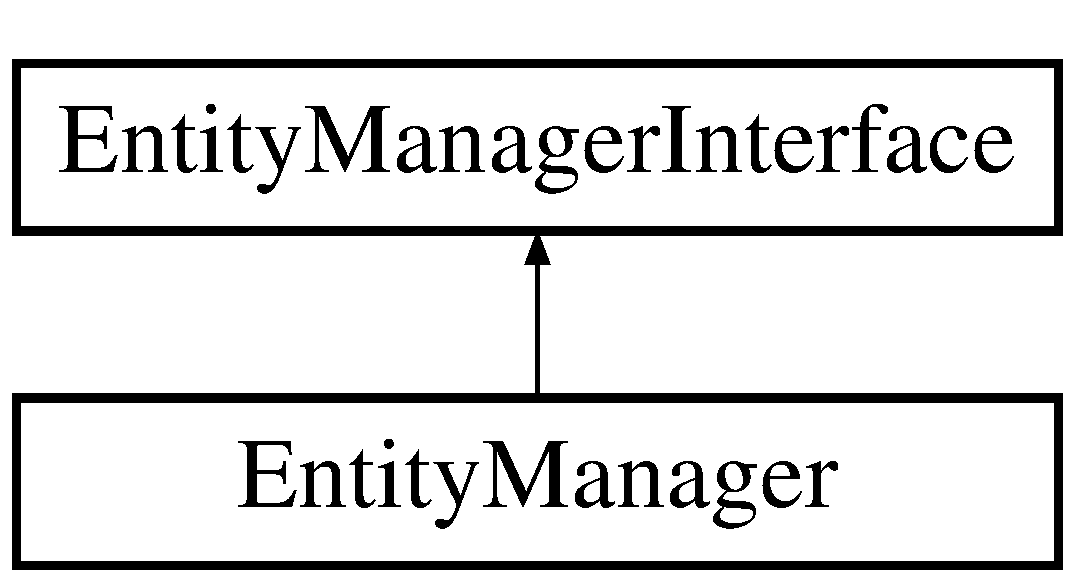
\includegraphics[height=2.000000cm]{classEntityManager}
\end{center}
\end{figure}
\subsection*{Public Member Functions}
\begin{DoxyCompactItemize}
\item 
void \hyperlink{classEntityManager_a97a7e5a629a5ffe85a2859384e5ce701}{initialise} (\hyperlink{classGameEngineInterface}{Game\-Engine\-Interface} $\ast$engine)
\item 
void \hyperlink{classEntityManager_af84b8842db8f732039c41dc4bc30b0c1}{destroy} ()
\item 
\hyperlink{classEntity}{Entity} $\ast$ \hyperlink{classEntityManager_af54f317708b43ec7c22be0495a8ce3c0}{create\-Entity} (const std\-::string \&name)
\item 
void \hyperlink{classEntityManager_afe54803a7170a4a2d2614348ed9f7cab}{destroy\-Entity} (\hyperlink{entity_8h_a3812b46f7256476cf244cbc0f4a3bde9}{Entity\-Id})
\item 
\hyperlink{classEntity}{Entity} $\ast$ \hyperlink{classEntityManager_a098b4e50944a8caffb723e7d0dffbb70}{get\-Player} ()
\item 
\hyperlink{classEntity}{Entity} $\ast$ \hyperlink{classEntityManager_a6d7f11fe8bfe9821377108874b6248e3}{create\-Wall\-Prefab} (unsigned int x, unsigned int y)
\item 
\hyperlink{classEntity}{Entity} $\ast$ \hyperlink{classEntityManager_aa450f3815645d947e41bec34fd7c628e}{create\-Player\-Prefab} (unsigned int x, unsigned int y)
\item 
\hyperlink{classEntity}{Entity} $\ast$ \hyperlink{classEntityManager_a8110b8b5376e15127609753e52bd779f}{create\-Enemy\-Prefab} (unsigned int x, unsigned int y)
\item 
\hyperlink{classEntity}{Entity} $\ast$ \hyperlink{classEntityManager_a37c9debe4a2ecb9316441ea19fdbe04e}{create\-Tile\-Prefab} (unsigned int x, unsigned int y)
\item 
\hyperlink{classComponentManagerInterface}{Component\-Manager\-Interface}\\*
$<$ \hyperlink{structSpriteComponent}{Sprite\-Component} $>$ $\ast$ \hyperlink{classEntityManager_a0af107dd34e63fa9e84d7b0e0e81d5ba}{get\-Sprites} ()
\item 
\hyperlink{classComponentManagerInterface}{Component\-Manager\-Interface}\\*
$<$ \hyperlink{structColliderComponent}{Collider\-Component} $>$ $\ast$ \hyperlink{classEntityManager_ab024c88ff91734e8ba57bba27c985dca}{get\-Colliders} ()
\item 
\hyperlink{classEntity}{Entity} $\ast$ \hyperlink{classEntityManager_a23e110f8bc01067e5bd953e8b7008273}{get\-Entity} (\hyperlink{entity_8h_a3812b46f7256476cf244cbc0f4a3bde9}{Entity\-Id} id)
\end{DoxyCompactItemize}
\subsection*{Private Attributes}
\begin{DoxyCompactItemize}
\item 
\hyperlink{classGameEngineInterface}{Game\-Engine\-Interface} $\ast$ \hyperlink{classEntityManager_aa6e686169c3667ffd84e6a3f0e2cfc62}{m\-\_\-engine}
\item 
unsigned long \hyperlink{classEntityManager_a73390a51b55cd69d0d09254894d484b3}{max\-Id}
\item 
\hyperlink{classEntity}{Entity} $\ast$ \hyperlink{classEntityManager_ac966d9cc295a8222c01a835246206d36}{m\-\_\-player}
\item 
std\-::map$<$ \hyperlink{entity_8h_a3812b46f7256476cf244cbc0f4a3bde9}{Entity\-Id}, \hyperlink{classEntity}{Entity} $\ast$ $>$ \hyperlink{classEntityManager_ab85b819de6db421c0272e76d5089bfbf}{m\-\_\-id\-Map}
\item 
std\-::map$<$ std\-::string, \hyperlink{classEntity}{Entity} $\ast$ $>$ \hyperlink{classEntityManager_aba0769f85d9f51fe54494ab68e1ebf0e}{m\-\_\-name\-Map}
\item 
\hyperlink{classComponentManager}{Component\-Manager}$<$ \hyperlink{structSpriteComponent}{Sprite\-Component} $>$ \hyperlink{classEntityManager_ab0ca6f699c4b0380acc8c0c2dd0fa778}{m\-\_\-sprites}
\item 
\hyperlink{classComponentManager}{Component\-Manager}\\*
$<$ \hyperlink{structColliderComponent}{Collider\-Component} $>$ \hyperlink{classEntityManager_acdcb4eaa4584972dcfe49dc11f08e196}{m\-\_\-colliders}
\end{DoxyCompactItemize}


\subsection{Member Function Documentation}
\hypertarget{classEntityManager_a8110b8b5376e15127609753e52bd779f}{\index{Entity\-Manager@{Entity\-Manager}!create\-Enemy\-Prefab@{create\-Enemy\-Prefab}}
\index{create\-Enemy\-Prefab@{create\-Enemy\-Prefab}!EntityManager@{Entity\-Manager}}
\subsubsection[{create\-Enemy\-Prefab}]{\setlength{\rightskip}{0pt plus 5cm}{\bf Entity} $\ast$ Entity\-Manager\-::create\-Enemy\-Prefab (
\begin{DoxyParamCaption}
\item[{unsigned int}]{x, }
\item[{unsigned int}]{y}
\end{DoxyParamCaption}
)\hspace{0.3cm}{\ttfamily [virtual]}}}\label{classEntityManager_a8110b8b5376e15127609753e52bd779f}


Implements \hyperlink{classEntityManagerInterface_a9060a65f6799126b3b7827bdd2636e92}{Entity\-Manager\-Interface}.

\hypertarget{classEntityManager_af54f317708b43ec7c22be0495a8ce3c0}{\index{Entity\-Manager@{Entity\-Manager}!create\-Entity@{create\-Entity}}
\index{create\-Entity@{create\-Entity}!EntityManager@{Entity\-Manager}}
\subsubsection[{create\-Entity}]{\setlength{\rightskip}{0pt plus 5cm}{\bf Entity} $\ast$ Entity\-Manager\-::create\-Entity (
\begin{DoxyParamCaption}
\item[{const std\-::string \&}]{name}
\end{DoxyParamCaption}
)\hspace{0.3cm}{\ttfamily [virtual]}}}\label{classEntityManager_af54f317708b43ec7c22be0495a8ce3c0}


Implements \hyperlink{classEntityManagerInterface_a95ba3a0c18e752b97de7b6a3ffd0301f}{Entity\-Manager\-Interface}.

\hypertarget{classEntityManager_aa450f3815645d947e41bec34fd7c628e}{\index{Entity\-Manager@{Entity\-Manager}!create\-Player\-Prefab@{create\-Player\-Prefab}}
\index{create\-Player\-Prefab@{create\-Player\-Prefab}!EntityManager@{Entity\-Manager}}
\subsubsection[{create\-Player\-Prefab}]{\setlength{\rightskip}{0pt plus 5cm}{\bf Entity} $\ast$ Entity\-Manager\-::create\-Player\-Prefab (
\begin{DoxyParamCaption}
\item[{unsigned int}]{x, }
\item[{unsigned int}]{y}
\end{DoxyParamCaption}
)\hspace{0.3cm}{\ttfamily [virtual]}}}\label{classEntityManager_aa450f3815645d947e41bec34fd7c628e}


Implements \hyperlink{classEntityManagerInterface_aca4bf34ec9006329027f134575a8b844}{Entity\-Manager\-Interface}.

\hypertarget{classEntityManager_a37c9debe4a2ecb9316441ea19fdbe04e}{\index{Entity\-Manager@{Entity\-Manager}!create\-Tile\-Prefab@{create\-Tile\-Prefab}}
\index{create\-Tile\-Prefab@{create\-Tile\-Prefab}!EntityManager@{Entity\-Manager}}
\subsubsection[{create\-Tile\-Prefab}]{\setlength{\rightskip}{0pt plus 5cm}{\bf Entity} $\ast$ Entity\-Manager\-::create\-Tile\-Prefab (
\begin{DoxyParamCaption}
\item[{unsigned int}]{x, }
\item[{unsigned int}]{y}
\end{DoxyParamCaption}
)\hspace{0.3cm}{\ttfamily [virtual]}}}\label{classEntityManager_a37c9debe4a2ecb9316441ea19fdbe04e}


Implements \hyperlink{classEntityManagerInterface_aa98d0ba0e59103d9aeb7a367fe04c571}{Entity\-Manager\-Interface}.

\hypertarget{classEntityManager_a6d7f11fe8bfe9821377108874b6248e3}{\index{Entity\-Manager@{Entity\-Manager}!create\-Wall\-Prefab@{create\-Wall\-Prefab}}
\index{create\-Wall\-Prefab@{create\-Wall\-Prefab}!EntityManager@{Entity\-Manager}}
\subsubsection[{create\-Wall\-Prefab}]{\setlength{\rightskip}{0pt plus 5cm}{\bf Entity} $\ast$ Entity\-Manager\-::create\-Wall\-Prefab (
\begin{DoxyParamCaption}
\item[{unsigned int}]{x, }
\item[{unsigned int}]{y}
\end{DoxyParamCaption}
)\hspace{0.3cm}{\ttfamily [virtual]}}}\label{classEntityManager_a6d7f11fe8bfe9821377108874b6248e3}


Implements \hyperlink{classEntityManagerInterface_a9aae8cf72f08ee33ea110325148ef613}{Entity\-Manager\-Interface}.

\hypertarget{classEntityManager_af84b8842db8f732039c41dc4bc30b0c1}{\index{Entity\-Manager@{Entity\-Manager}!destroy@{destroy}}
\index{destroy@{destroy}!EntityManager@{Entity\-Manager}}
\subsubsection[{destroy}]{\setlength{\rightskip}{0pt plus 5cm}void Entity\-Manager\-::destroy (
\begin{DoxyParamCaption}
{}
\end{DoxyParamCaption}
)\hspace{0.3cm}{\ttfamily [inline]}, {\ttfamily [virtual]}}}\label{classEntityManager_af84b8842db8f732039c41dc4bc30b0c1}


Implements \hyperlink{classEntityManagerInterface_ab27d9f7d97a914785cc5955076c10d70}{Entity\-Manager\-Interface}.

\hypertarget{classEntityManager_afe54803a7170a4a2d2614348ed9f7cab}{\index{Entity\-Manager@{Entity\-Manager}!destroy\-Entity@{destroy\-Entity}}
\index{destroy\-Entity@{destroy\-Entity}!EntityManager@{Entity\-Manager}}
\subsubsection[{destroy\-Entity}]{\setlength{\rightskip}{0pt plus 5cm}void Entity\-Manager\-::destroy\-Entity (
\begin{DoxyParamCaption}
\item[{{\bf Entity\-Id}}]{id}
\end{DoxyParamCaption}
)\hspace{0.3cm}{\ttfamily [virtual]}}}\label{classEntityManager_afe54803a7170a4a2d2614348ed9f7cab}


Implements \hyperlink{classEntityManagerInterface_a01d56437b2df1ba882da83e5f6aaa163}{Entity\-Manager\-Interface}.

\hypertarget{classEntityManager_ab024c88ff91734e8ba57bba27c985dca}{\index{Entity\-Manager@{Entity\-Manager}!get\-Colliders@{get\-Colliders}}
\index{get\-Colliders@{get\-Colliders}!EntityManager@{Entity\-Manager}}
\subsubsection[{get\-Colliders}]{\setlength{\rightskip}{0pt plus 5cm}{\bf Component\-Manager\-Interface}$<${\bf Collider\-Component}$>$$\ast$ Entity\-Manager\-::get\-Colliders (
\begin{DoxyParamCaption}
{}
\end{DoxyParamCaption}
)\hspace{0.3cm}{\ttfamily [inline]}, {\ttfamily [virtual]}}}\label{classEntityManager_ab024c88ff91734e8ba57bba27c985dca}


Implements \hyperlink{classEntityManagerInterface_acc684c426594345b02b206efb74b0adc}{Entity\-Manager\-Interface}.

\hypertarget{classEntityManager_a23e110f8bc01067e5bd953e8b7008273}{\index{Entity\-Manager@{Entity\-Manager}!get\-Entity@{get\-Entity}}
\index{get\-Entity@{get\-Entity}!EntityManager@{Entity\-Manager}}
\subsubsection[{get\-Entity}]{\setlength{\rightskip}{0pt plus 5cm}{\bf Entity} $\ast$ Entity\-Manager\-::get\-Entity (
\begin{DoxyParamCaption}
\item[{{\bf Entity\-Id}}]{id}
\end{DoxyParamCaption}
)\hspace{0.3cm}{\ttfamily [virtual]}}}\label{classEntityManager_a23e110f8bc01067e5bd953e8b7008273}


Implements \hyperlink{classEntityManagerInterface_a00346fa684da1972fbd086599b949ed9}{Entity\-Manager\-Interface}.

\hypertarget{classEntityManager_a098b4e50944a8caffb723e7d0dffbb70}{\index{Entity\-Manager@{Entity\-Manager}!get\-Player@{get\-Player}}
\index{get\-Player@{get\-Player}!EntityManager@{Entity\-Manager}}
\subsubsection[{get\-Player}]{\setlength{\rightskip}{0pt plus 5cm}{\bf Entity} $\ast$ Entity\-Manager\-::get\-Player (
\begin{DoxyParamCaption}
{}
\end{DoxyParamCaption}
)\hspace{0.3cm}{\ttfamily [virtual]}}}\label{classEntityManager_a098b4e50944a8caffb723e7d0dffbb70}


Implements \hyperlink{classEntityManagerInterface_af59c4f44e337dc04fd7aac61e80b2660}{Entity\-Manager\-Interface}.

\hypertarget{classEntityManager_a0af107dd34e63fa9e84d7b0e0e81d5ba}{\index{Entity\-Manager@{Entity\-Manager}!get\-Sprites@{get\-Sprites}}
\index{get\-Sprites@{get\-Sprites}!EntityManager@{Entity\-Manager}}
\subsubsection[{get\-Sprites}]{\setlength{\rightskip}{0pt plus 5cm}{\bf Component\-Manager\-Interface}$<${\bf Sprite\-Component}$>$$\ast$ Entity\-Manager\-::get\-Sprites (
\begin{DoxyParamCaption}
{}
\end{DoxyParamCaption}
)\hspace{0.3cm}{\ttfamily [inline]}, {\ttfamily [virtual]}}}\label{classEntityManager_a0af107dd34e63fa9e84d7b0e0e81d5ba}


Implements \hyperlink{classEntityManagerInterface_a91bd6cea03b2b69ddec735e116420dd6}{Entity\-Manager\-Interface}.

\hypertarget{classEntityManager_a97a7e5a629a5ffe85a2859384e5ce701}{\index{Entity\-Manager@{Entity\-Manager}!initialise@{initialise}}
\index{initialise@{initialise}!EntityManager@{Entity\-Manager}}
\subsubsection[{initialise}]{\setlength{\rightskip}{0pt plus 5cm}void Entity\-Manager\-::initialise (
\begin{DoxyParamCaption}
\item[{{\bf Game\-Engine\-Interface} $\ast$}]{engine}
\end{DoxyParamCaption}
)\hspace{0.3cm}{\ttfamily [virtual]}}}\label{classEntityManager_a97a7e5a629a5ffe85a2859384e5ce701}


Implements \hyperlink{classEntityManagerInterface_aeb1fd14604e776e874765fa708a7ce26}{Entity\-Manager\-Interface}.



\subsection{Member Data Documentation}
\hypertarget{classEntityManager_acdcb4eaa4584972dcfe49dc11f08e196}{\index{Entity\-Manager@{Entity\-Manager}!m\-\_\-colliders@{m\-\_\-colliders}}
\index{m\-\_\-colliders@{m\-\_\-colliders}!EntityManager@{Entity\-Manager}}
\subsubsection[{m\-\_\-colliders}]{\setlength{\rightskip}{0pt plus 5cm}{\bf Component\-Manager}$<${\bf Collider\-Component}$>$ Entity\-Manager\-::m\-\_\-colliders\hspace{0.3cm}{\ttfamily [private]}}}\label{classEntityManager_acdcb4eaa4584972dcfe49dc11f08e196}
\hypertarget{classEntityManager_aa6e686169c3667ffd84e6a3f0e2cfc62}{\index{Entity\-Manager@{Entity\-Manager}!m\-\_\-engine@{m\-\_\-engine}}
\index{m\-\_\-engine@{m\-\_\-engine}!EntityManager@{Entity\-Manager}}
\subsubsection[{m\-\_\-engine}]{\setlength{\rightskip}{0pt plus 5cm}{\bf Game\-Engine\-Interface}$\ast$ Entity\-Manager\-::m\-\_\-engine\hspace{0.3cm}{\ttfamily [private]}}}\label{classEntityManager_aa6e686169c3667ffd84e6a3f0e2cfc62}
\hypertarget{classEntityManager_ab85b819de6db421c0272e76d5089bfbf}{\index{Entity\-Manager@{Entity\-Manager}!m\-\_\-id\-Map@{m\-\_\-id\-Map}}
\index{m\-\_\-id\-Map@{m\-\_\-id\-Map}!EntityManager@{Entity\-Manager}}
\subsubsection[{m\-\_\-id\-Map}]{\setlength{\rightskip}{0pt plus 5cm}std\-::map$<${\bf Entity\-Id}, {\bf Entity}$\ast$$>$ Entity\-Manager\-::m\-\_\-id\-Map\hspace{0.3cm}{\ttfamily [private]}}}\label{classEntityManager_ab85b819de6db421c0272e76d5089bfbf}
\hypertarget{classEntityManager_aba0769f85d9f51fe54494ab68e1ebf0e}{\index{Entity\-Manager@{Entity\-Manager}!m\-\_\-name\-Map@{m\-\_\-name\-Map}}
\index{m\-\_\-name\-Map@{m\-\_\-name\-Map}!EntityManager@{Entity\-Manager}}
\subsubsection[{m\-\_\-name\-Map}]{\setlength{\rightskip}{0pt plus 5cm}std\-::map$<$std\-::string, {\bf Entity}$\ast$$>$ Entity\-Manager\-::m\-\_\-name\-Map\hspace{0.3cm}{\ttfamily [private]}}}\label{classEntityManager_aba0769f85d9f51fe54494ab68e1ebf0e}
\hypertarget{classEntityManager_ac966d9cc295a8222c01a835246206d36}{\index{Entity\-Manager@{Entity\-Manager}!m\-\_\-player@{m\-\_\-player}}
\index{m\-\_\-player@{m\-\_\-player}!EntityManager@{Entity\-Manager}}
\subsubsection[{m\-\_\-player}]{\setlength{\rightskip}{0pt plus 5cm}{\bf Entity}$\ast$ Entity\-Manager\-::m\-\_\-player\hspace{0.3cm}{\ttfamily [private]}}}\label{classEntityManager_ac966d9cc295a8222c01a835246206d36}
\hypertarget{classEntityManager_ab0ca6f699c4b0380acc8c0c2dd0fa778}{\index{Entity\-Manager@{Entity\-Manager}!m\-\_\-sprites@{m\-\_\-sprites}}
\index{m\-\_\-sprites@{m\-\_\-sprites}!EntityManager@{Entity\-Manager}}
\subsubsection[{m\-\_\-sprites}]{\setlength{\rightskip}{0pt plus 5cm}{\bf Component\-Manager}$<${\bf Sprite\-Component}$>$ Entity\-Manager\-::m\-\_\-sprites\hspace{0.3cm}{\ttfamily [private]}}}\label{classEntityManager_ab0ca6f699c4b0380acc8c0c2dd0fa778}
\hypertarget{classEntityManager_a73390a51b55cd69d0d09254894d484b3}{\index{Entity\-Manager@{Entity\-Manager}!max\-Id@{max\-Id}}
\index{max\-Id@{max\-Id}!EntityManager@{Entity\-Manager}}
\subsubsection[{max\-Id}]{\setlength{\rightskip}{0pt plus 5cm}unsigned long Entity\-Manager\-::max\-Id\hspace{0.3cm}{\ttfamily [private]}}}\label{classEntityManager_a73390a51b55cd69d0d09254894d484b3}


The documentation for this class was generated from the following files\-:\begin{DoxyCompactItemize}
\item 
\hyperlink{entity__manager_8h}{entity\-\_\-manager.\-h}\item 
\hyperlink{entity__manager_8cpp}{entity\-\_\-manager.\-cpp}\end{DoxyCompactItemize}

\hypertarget{classEntityManagerInterface}{\section{Entity\-Manager\-Interface Class Reference}
\label{classEntityManagerInterface}\index{Entity\-Manager\-Interface@{Entity\-Manager\-Interface}}
}


{\ttfamily \#include $<$entity\-\_\-manager\-\_\-interface.\-h$>$}

Inheritance diagram for Entity\-Manager\-Interface\-:\begin{figure}[H]
\begin{center}
\leavevmode
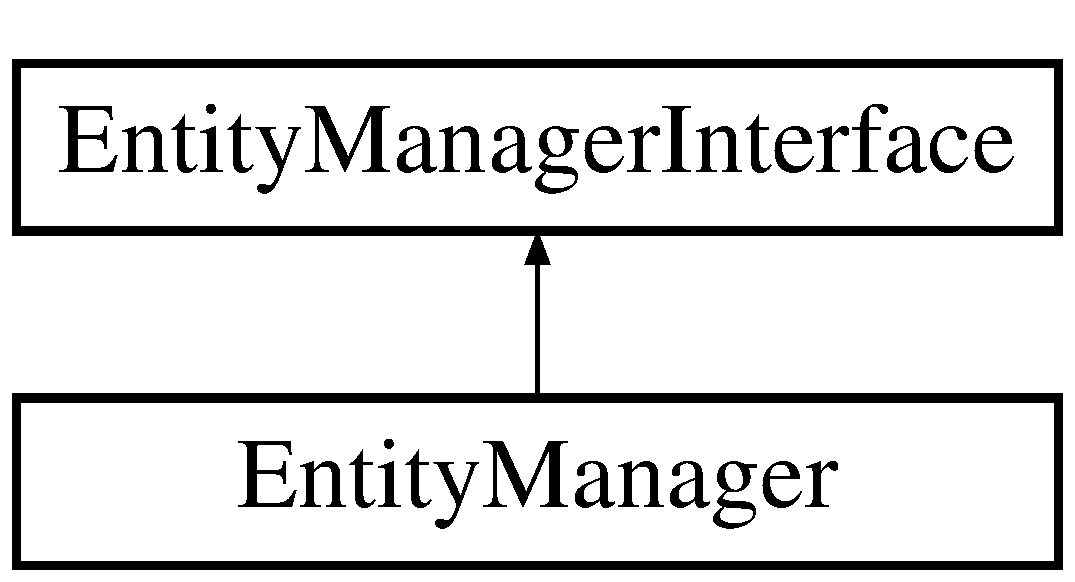
\includegraphics[height=2.000000cm]{classEntityManagerInterface}
\end{center}
\end{figure}
\subsection*{Public Member Functions}
\begin{DoxyCompactItemize}
\item 
virtual \hyperlink{classEntityManagerInterface_a4991d0d31ad6f551335bbc2c65383a9f}{$\sim$\-Entity\-Manager\-Interface} ()
\item 
virtual void \hyperlink{classEntityManagerInterface_aeb1fd14604e776e874765fa708a7ce26}{initialise} (\hyperlink{classGameEngineInterface}{Game\-Engine\-Interface} $\ast$engine)=0
\item 
virtual void \hyperlink{classEntityManagerInterface_ab27d9f7d97a914785cc5955076c10d70}{destroy} ()=0
\item 
virtual \hyperlink{classEntity}{Entity} $\ast$ \hyperlink{classEntityManagerInterface_a95ba3a0c18e752b97de7b6a3ffd0301f}{create\-Entity} (const std\-::string \&name)=0
\item 
virtual void \hyperlink{classEntityManagerInterface_a01d56437b2df1ba882da83e5f6aaa163}{destroy\-Entity} (\hyperlink{entity_8h_a3812b46f7256476cf244cbc0f4a3bde9}{Entity\-Id} id)=0
\item 
virtual \hyperlink{classEntity}{Entity} $\ast$ \hyperlink{classEntityManagerInterface_af59c4f44e337dc04fd7aac61e80b2660}{get\-Player} ()=0
\item 
virtual \hyperlink{classEntity}{Entity} $\ast$ \hyperlink{classEntityManagerInterface_a9aae8cf72f08ee33ea110325148ef613}{create\-Wall\-Prefab} (unsigned int x, unsigned int y)=0
\item 
virtual \hyperlink{classEntity}{Entity} $\ast$ \hyperlink{classEntityManagerInterface_aca4bf34ec9006329027f134575a8b844}{create\-Player\-Prefab} (unsigned int x, unsigned int y)=0
\item 
virtual \hyperlink{classEntity}{Entity} $\ast$ \hyperlink{classEntityManagerInterface_a9060a65f6799126b3b7827bdd2636e92}{create\-Enemy\-Prefab} (unsigned int x, unsigned int y)=0
\item 
virtual \hyperlink{classEntity}{Entity} $\ast$ \hyperlink{classEntityManagerInterface_aa98d0ba0e59103d9aeb7a367fe04c571}{create\-Tile\-Prefab} (unsigned int x, unsigned int y)=0
\item 
virtual \\*
\hyperlink{classComponentManagerInterface}{Component\-Manager\-Interface}\\*
$<$ \hyperlink{structSpriteComponent}{Sprite\-Component} $>$ $\ast$ \hyperlink{classEntityManagerInterface_a91bd6cea03b2b69ddec735e116420dd6}{get\-Sprites} ()=0
\item 
virtual \\*
\hyperlink{classComponentManagerInterface}{Component\-Manager\-Interface}\\*
$<$ \hyperlink{structColliderComponent}{Collider\-Component} $>$ $\ast$ \hyperlink{classEntityManagerInterface_acc684c426594345b02b206efb74b0adc}{get\-Colliders} ()=0
\item 
virtual \hyperlink{classEntity}{Entity} $\ast$ \hyperlink{classEntityManagerInterface_a00346fa684da1972fbd086599b949ed9}{get\-Entity} (\hyperlink{entity_8h_a3812b46f7256476cf244cbc0f4a3bde9}{Entity\-Id} id)=0
\end{DoxyCompactItemize}


\subsection{Constructor \& Destructor Documentation}
\hypertarget{classEntityManagerInterface_a4991d0d31ad6f551335bbc2c65383a9f}{\index{Entity\-Manager\-Interface@{Entity\-Manager\-Interface}!$\sim$\-Entity\-Manager\-Interface@{$\sim$\-Entity\-Manager\-Interface}}
\index{$\sim$\-Entity\-Manager\-Interface@{$\sim$\-Entity\-Manager\-Interface}!EntityManagerInterface@{Entity\-Manager\-Interface}}
\subsubsection[{$\sim$\-Entity\-Manager\-Interface}]{\setlength{\rightskip}{0pt plus 5cm}virtual Entity\-Manager\-Interface\-::$\sim$\-Entity\-Manager\-Interface (
\begin{DoxyParamCaption}
{}
\end{DoxyParamCaption}
)\hspace{0.3cm}{\ttfamily [inline]}, {\ttfamily [virtual]}}}\label{classEntityManagerInterface_a4991d0d31ad6f551335bbc2c65383a9f}


\subsection{Member Function Documentation}
\hypertarget{classEntityManagerInterface_a9060a65f6799126b3b7827bdd2636e92}{\index{Entity\-Manager\-Interface@{Entity\-Manager\-Interface}!create\-Enemy\-Prefab@{create\-Enemy\-Prefab}}
\index{create\-Enemy\-Prefab@{create\-Enemy\-Prefab}!EntityManagerInterface@{Entity\-Manager\-Interface}}
\subsubsection[{create\-Enemy\-Prefab}]{\setlength{\rightskip}{0pt plus 5cm}virtual {\bf Entity}$\ast$ Entity\-Manager\-Interface\-::create\-Enemy\-Prefab (
\begin{DoxyParamCaption}
\item[{unsigned int}]{x, }
\item[{unsigned int}]{y}
\end{DoxyParamCaption}
)\hspace{0.3cm}{\ttfamily [pure virtual]}}}\label{classEntityManagerInterface_a9060a65f6799126b3b7827bdd2636e92}


Implemented in \hyperlink{classEntityManager_a8110b8b5376e15127609753e52bd779f}{Entity\-Manager}.

\hypertarget{classEntityManagerInterface_a95ba3a0c18e752b97de7b6a3ffd0301f}{\index{Entity\-Manager\-Interface@{Entity\-Manager\-Interface}!create\-Entity@{create\-Entity}}
\index{create\-Entity@{create\-Entity}!EntityManagerInterface@{Entity\-Manager\-Interface}}
\subsubsection[{create\-Entity}]{\setlength{\rightskip}{0pt plus 5cm}virtual {\bf Entity}$\ast$ Entity\-Manager\-Interface\-::create\-Entity (
\begin{DoxyParamCaption}
\item[{const std\-::string \&}]{name}
\end{DoxyParamCaption}
)\hspace{0.3cm}{\ttfamily [pure virtual]}}}\label{classEntityManagerInterface_a95ba3a0c18e752b97de7b6a3ffd0301f}


Implemented in \hyperlink{classEntityManager_af54f317708b43ec7c22be0495a8ce3c0}{Entity\-Manager}.

\hypertarget{classEntityManagerInterface_aca4bf34ec9006329027f134575a8b844}{\index{Entity\-Manager\-Interface@{Entity\-Manager\-Interface}!create\-Player\-Prefab@{create\-Player\-Prefab}}
\index{create\-Player\-Prefab@{create\-Player\-Prefab}!EntityManagerInterface@{Entity\-Manager\-Interface}}
\subsubsection[{create\-Player\-Prefab}]{\setlength{\rightskip}{0pt plus 5cm}virtual {\bf Entity}$\ast$ Entity\-Manager\-Interface\-::create\-Player\-Prefab (
\begin{DoxyParamCaption}
\item[{unsigned int}]{x, }
\item[{unsigned int}]{y}
\end{DoxyParamCaption}
)\hspace{0.3cm}{\ttfamily [pure virtual]}}}\label{classEntityManagerInterface_aca4bf34ec9006329027f134575a8b844}


Implemented in \hyperlink{classEntityManager_aa450f3815645d947e41bec34fd7c628e}{Entity\-Manager}.

\hypertarget{classEntityManagerInterface_aa98d0ba0e59103d9aeb7a367fe04c571}{\index{Entity\-Manager\-Interface@{Entity\-Manager\-Interface}!create\-Tile\-Prefab@{create\-Tile\-Prefab}}
\index{create\-Tile\-Prefab@{create\-Tile\-Prefab}!EntityManagerInterface@{Entity\-Manager\-Interface}}
\subsubsection[{create\-Tile\-Prefab}]{\setlength{\rightskip}{0pt plus 5cm}virtual {\bf Entity}$\ast$ Entity\-Manager\-Interface\-::create\-Tile\-Prefab (
\begin{DoxyParamCaption}
\item[{unsigned int}]{x, }
\item[{unsigned int}]{y}
\end{DoxyParamCaption}
)\hspace{0.3cm}{\ttfamily [pure virtual]}}}\label{classEntityManagerInterface_aa98d0ba0e59103d9aeb7a367fe04c571}


Implemented in \hyperlink{classEntityManager_a37c9debe4a2ecb9316441ea19fdbe04e}{Entity\-Manager}.

\hypertarget{classEntityManagerInterface_a9aae8cf72f08ee33ea110325148ef613}{\index{Entity\-Manager\-Interface@{Entity\-Manager\-Interface}!create\-Wall\-Prefab@{create\-Wall\-Prefab}}
\index{create\-Wall\-Prefab@{create\-Wall\-Prefab}!EntityManagerInterface@{Entity\-Manager\-Interface}}
\subsubsection[{create\-Wall\-Prefab}]{\setlength{\rightskip}{0pt plus 5cm}virtual {\bf Entity}$\ast$ Entity\-Manager\-Interface\-::create\-Wall\-Prefab (
\begin{DoxyParamCaption}
\item[{unsigned int}]{x, }
\item[{unsigned int}]{y}
\end{DoxyParamCaption}
)\hspace{0.3cm}{\ttfamily [pure virtual]}}}\label{classEntityManagerInterface_a9aae8cf72f08ee33ea110325148ef613}


Implemented in \hyperlink{classEntityManager_a6d7f11fe8bfe9821377108874b6248e3}{Entity\-Manager}.

\hypertarget{classEntityManagerInterface_ab27d9f7d97a914785cc5955076c10d70}{\index{Entity\-Manager\-Interface@{Entity\-Manager\-Interface}!destroy@{destroy}}
\index{destroy@{destroy}!EntityManagerInterface@{Entity\-Manager\-Interface}}
\subsubsection[{destroy}]{\setlength{\rightskip}{0pt plus 5cm}virtual void Entity\-Manager\-Interface\-::destroy (
\begin{DoxyParamCaption}
{}
\end{DoxyParamCaption}
)\hspace{0.3cm}{\ttfamily [pure virtual]}}}\label{classEntityManagerInterface_ab27d9f7d97a914785cc5955076c10d70}


Implemented in \hyperlink{classEntityManager_af84b8842db8f732039c41dc4bc30b0c1}{Entity\-Manager}.

\hypertarget{classEntityManagerInterface_a01d56437b2df1ba882da83e5f6aaa163}{\index{Entity\-Manager\-Interface@{Entity\-Manager\-Interface}!destroy\-Entity@{destroy\-Entity}}
\index{destroy\-Entity@{destroy\-Entity}!EntityManagerInterface@{Entity\-Manager\-Interface}}
\subsubsection[{destroy\-Entity}]{\setlength{\rightskip}{0pt plus 5cm}virtual void Entity\-Manager\-Interface\-::destroy\-Entity (
\begin{DoxyParamCaption}
\item[{{\bf Entity\-Id}}]{id}
\end{DoxyParamCaption}
)\hspace{0.3cm}{\ttfamily [pure virtual]}}}\label{classEntityManagerInterface_a01d56437b2df1ba882da83e5f6aaa163}


Implemented in \hyperlink{classEntityManager_afe54803a7170a4a2d2614348ed9f7cab}{Entity\-Manager}.

\hypertarget{classEntityManagerInterface_acc684c426594345b02b206efb74b0adc}{\index{Entity\-Manager\-Interface@{Entity\-Manager\-Interface}!get\-Colliders@{get\-Colliders}}
\index{get\-Colliders@{get\-Colliders}!EntityManagerInterface@{Entity\-Manager\-Interface}}
\subsubsection[{get\-Colliders}]{\setlength{\rightskip}{0pt plus 5cm}virtual {\bf Component\-Manager\-Interface}$<${\bf Collider\-Component}$>$$\ast$ Entity\-Manager\-Interface\-::get\-Colliders (
\begin{DoxyParamCaption}
{}
\end{DoxyParamCaption}
)\hspace{0.3cm}{\ttfamily [pure virtual]}}}\label{classEntityManagerInterface_acc684c426594345b02b206efb74b0adc}


Implemented in \hyperlink{classEntityManager_ab024c88ff91734e8ba57bba27c985dca}{Entity\-Manager}.

\hypertarget{classEntityManagerInterface_a00346fa684da1972fbd086599b949ed9}{\index{Entity\-Manager\-Interface@{Entity\-Manager\-Interface}!get\-Entity@{get\-Entity}}
\index{get\-Entity@{get\-Entity}!EntityManagerInterface@{Entity\-Manager\-Interface}}
\subsubsection[{get\-Entity}]{\setlength{\rightskip}{0pt plus 5cm}virtual {\bf Entity}$\ast$ Entity\-Manager\-Interface\-::get\-Entity (
\begin{DoxyParamCaption}
\item[{{\bf Entity\-Id}}]{id}
\end{DoxyParamCaption}
)\hspace{0.3cm}{\ttfamily [pure virtual]}}}\label{classEntityManagerInterface_a00346fa684da1972fbd086599b949ed9}


Implemented in \hyperlink{classEntityManager_a23e110f8bc01067e5bd953e8b7008273}{Entity\-Manager}.

\hypertarget{classEntityManagerInterface_af59c4f44e337dc04fd7aac61e80b2660}{\index{Entity\-Manager\-Interface@{Entity\-Manager\-Interface}!get\-Player@{get\-Player}}
\index{get\-Player@{get\-Player}!EntityManagerInterface@{Entity\-Manager\-Interface}}
\subsubsection[{get\-Player}]{\setlength{\rightskip}{0pt plus 5cm}virtual {\bf Entity}$\ast$ Entity\-Manager\-Interface\-::get\-Player (
\begin{DoxyParamCaption}
{}
\end{DoxyParamCaption}
)\hspace{0.3cm}{\ttfamily [pure virtual]}}}\label{classEntityManagerInterface_af59c4f44e337dc04fd7aac61e80b2660}


Implemented in \hyperlink{classEntityManager_a098b4e50944a8caffb723e7d0dffbb70}{Entity\-Manager}.

\hypertarget{classEntityManagerInterface_a91bd6cea03b2b69ddec735e116420dd6}{\index{Entity\-Manager\-Interface@{Entity\-Manager\-Interface}!get\-Sprites@{get\-Sprites}}
\index{get\-Sprites@{get\-Sprites}!EntityManagerInterface@{Entity\-Manager\-Interface}}
\subsubsection[{get\-Sprites}]{\setlength{\rightskip}{0pt plus 5cm}virtual {\bf Component\-Manager\-Interface}$<${\bf Sprite\-Component}$>$$\ast$ Entity\-Manager\-Interface\-::get\-Sprites (
\begin{DoxyParamCaption}
{}
\end{DoxyParamCaption}
)\hspace{0.3cm}{\ttfamily [pure virtual]}}}\label{classEntityManagerInterface_a91bd6cea03b2b69ddec735e116420dd6}


Implemented in \hyperlink{classEntityManager_a0af107dd34e63fa9e84d7b0e0e81d5ba}{Entity\-Manager}.

\hypertarget{classEntityManagerInterface_aeb1fd14604e776e874765fa708a7ce26}{\index{Entity\-Manager\-Interface@{Entity\-Manager\-Interface}!initialise@{initialise}}
\index{initialise@{initialise}!EntityManagerInterface@{Entity\-Manager\-Interface}}
\subsubsection[{initialise}]{\setlength{\rightskip}{0pt plus 5cm}virtual void Entity\-Manager\-Interface\-::initialise (
\begin{DoxyParamCaption}
\item[{{\bf Game\-Engine\-Interface} $\ast$}]{engine}
\end{DoxyParamCaption}
)\hspace{0.3cm}{\ttfamily [pure virtual]}}}\label{classEntityManagerInterface_aeb1fd14604e776e874765fa708a7ce26}


Implemented in \hyperlink{classEntityManager_a97a7e5a629a5ffe85a2859384e5ce701}{Entity\-Manager}.



The documentation for this class was generated from the following file\-:\begin{DoxyCompactItemize}
\item 
\hyperlink{entity__manager__interface_8h}{entity\-\_\-manager\-\_\-interface.\-h}\end{DoxyCompactItemize}

\hypertarget{classEvent}{\section{Event Class Reference}
\label{classEvent}\index{Event@{Event}}
}


{\ttfamily \#include $<$event.\-h$>$}

Inheritance diagram for Event\-:\begin{figure}[H]
\begin{center}
\leavevmode
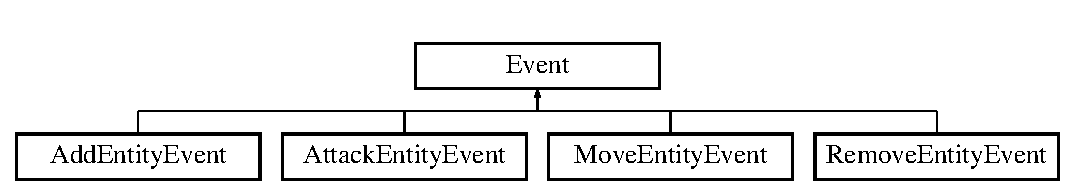
\includegraphics[height=2.000000cm]{classEvent}
\end{center}
\end{figure}
\subsection*{Public Member Functions}
\begin{DoxyCompactItemize}
\item 
\hyperlink{classEvent_aa3b8f22d374f6abfe0893bccea58a5de}{Event} (\hyperlink{event_8h_a2628ea8d12e8b2563c32f05dc7fff6fa}{Event\-Type} type)
\item 
virtual \hyperlink{classEvent_ab864fd85c758006c42cd7a1b3369b483}{$\sim$\-Event} ()
\item 
\hyperlink{event_8h_a2628ea8d12e8b2563c32f05dc7fff6fa}{Event\-Type} \hyperlink{classEvent_ab0c2e30730d5859851f3126258c0126e}{get\-Type} () const 
\end{DoxyCompactItemize}
\subsection*{Protected Attributes}
\begin{DoxyCompactItemize}
\item 
\hyperlink{event_8h_a2628ea8d12e8b2563c32f05dc7fff6fa}{Event\-Type} \hyperlink{classEvent_a38264e3fb229dc64123dff1d5a7dcf9e}{m\-\_\-type}
\end{DoxyCompactItemize}


\subsection{Constructor \& Destructor Documentation}
\hypertarget{classEvent_aa3b8f22d374f6abfe0893bccea58a5de}{\index{Event@{Event}!Event@{Event}}
\index{Event@{Event}!Event@{Event}}
\subsubsection[{Event}]{\setlength{\rightskip}{0pt plus 5cm}Event\-::\-Event (
\begin{DoxyParamCaption}
\item[{{\bf Event\-Type}}]{type}
\end{DoxyParamCaption}
)\hspace{0.3cm}{\ttfamily [inline]}}}\label{classEvent_aa3b8f22d374f6abfe0893bccea58a5de}
\hypertarget{classEvent_ab864fd85c758006c42cd7a1b3369b483}{\index{Event@{Event}!$\sim$\-Event@{$\sim$\-Event}}
\index{$\sim$\-Event@{$\sim$\-Event}!Event@{Event}}
\subsubsection[{$\sim$\-Event}]{\setlength{\rightskip}{0pt plus 5cm}virtual Event\-::$\sim$\-Event (
\begin{DoxyParamCaption}
{}
\end{DoxyParamCaption}
)\hspace{0.3cm}{\ttfamily [inline]}, {\ttfamily [virtual]}}}\label{classEvent_ab864fd85c758006c42cd7a1b3369b483}


\subsection{Member Function Documentation}
\hypertarget{classEvent_ab0c2e30730d5859851f3126258c0126e}{\index{Event@{Event}!get\-Type@{get\-Type}}
\index{get\-Type@{get\-Type}!Event@{Event}}
\subsubsection[{get\-Type}]{\setlength{\rightskip}{0pt plus 5cm}{\bf Event\-Type} Event\-::get\-Type (
\begin{DoxyParamCaption}
{}
\end{DoxyParamCaption}
) const\hspace{0.3cm}{\ttfamily [inline]}}}\label{classEvent_ab0c2e30730d5859851f3126258c0126e}


\subsection{Member Data Documentation}
\hypertarget{classEvent_a38264e3fb229dc64123dff1d5a7dcf9e}{\index{Event@{Event}!m\-\_\-type@{m\-\_\-type}}
\index{m\-\_\-type@{m\-\_\-type}!Event@{Event}}
\subsubsection[{m\-\_\-type}]{\setlength{\rightskip}{0pt plus 5cm}{\bf Event\-Type} Event\-::m\-\_\-type\hspace{0.3cm}{\ttfamily [protected]}}}\label{classEvent_a38264e3fb229dc64123dff1d5a7dcf9e}


The documentation for this class was generated from the following file\-:\begin{DoxyCompactItemize}
\item 
\hyperlink{event_8h}{event.\-h}\end{DoxyCompactItemize}

\hypertarget{classEventManager}{\section{Event\-Manager Class Reference}
\label{classEventManager}\index{Event\-Manager@{Event\-Manager}}
}


{\ttfamily \#include $<$event\-\_\-manager.\-h$>$}

Inheritance diagram for Event\-Manager\-:\begin{figure}[H]
\begin{center}
\leavevmode
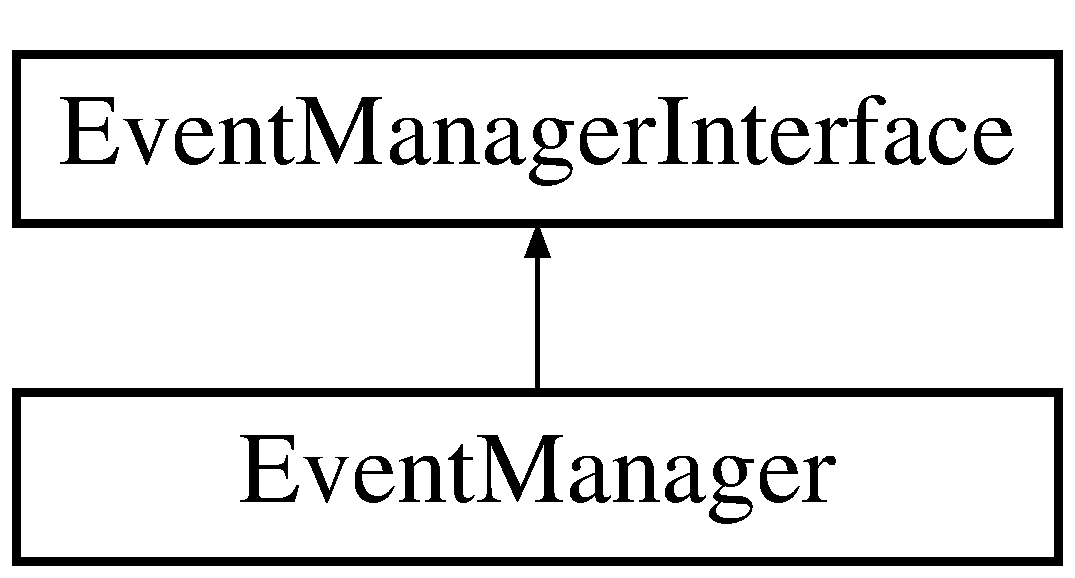
\includegraphics[height=2.000000cm]{classEventManager}
\end{center}
\end{figure}
\subsection*{Public Member Functions}
\begin{DoxyCompactItemize}
\item 
void \hyperlink{classEventManager_a93b64a8bc38a9842d10ee1526016671f}{initialise} (\hyperlink{classGameEngineInterface}{Game\-Engine\-Interface} $\ast$engine)
\item 
void \hyperlink{classEventManager_ae7c1bd23bc1beafa64b748553b471dce}{register\-Handler} (\hyperlink{classGameSystemInterface}{Game\-System\-Interface} $\ast$system)
\item 
void \hyperlink{classEventManager_abce64060a5fb8cc3d51803b0d43f222f}{raise\-Event} (\hyperlink{classEvent}{Event} $\ast$event)
\item 
void \hyperlink{classEventManager_ad40f65674444d1944159dd85888740d3}{process\-Events} ()
\end{DoxyCompactItemize}
\subsection*{Private Attributes}
\begin{DoxyCompactItemize}
\item 
\hyperlink{classGameEngineInterface}{Game\-Engine\-Interface} $\ast$ \hyperlink{classEventManager_ab26aa30e5a4ceb6f8c604b81991e7c39}{m\-\_\-engine}
\item 
\hyperlink{event__manager_8h_aa72a6ddd7c2b54a7df7b25928521b296}{Event\-Queue} \hyperlink{classEventManager_abc0dbcdc9126d867671acb49c48f6d36}{m\-\_\-events}
\item 
\hyperlink{event__manager_8h_a4d71a6d029a74348b1e4fbdc42f7acbd}{Handlers} \hyperlink{classEventManager_a0d6a8d7439edfb5e23402437ea0f1c4c}{m\-\_\-handlers}
\end{DoxyCompactItemize}


\subsection{Member Function Documentation}
\hypertarget{classEventManager_a93b64a8bc38a9842d10ee1526016671f}{\index{Event\-Manager@{Event\-Manager}!initialise@{initialise}}
\index{initialise@{initialise}!EventManager@{Event\-Manager}}
\subsubsection[{initialise}]{\setlength{\rightskip}{0pt plus 5cm}void Event\-Manager\-::initialise (
\begin{DoxyParamCaption}
\item[{{\bf Game\-Engine\-Interface} $\ast$}]{engine}
\end{DoxyParamCaption}
)\hspace{0.3cm}{\ttfamily [inline]}, {\ttfamily [virtual]}}}\label{classEventManager_a93b64a8bc38a9842d10ee1526016671f}


Implements \hyperlink{classEventManagerInterface_a13e851b9fa61887ab99dc0bba907bd05}{Event\-Manager\-Interface}.

\hypertarget{classEventManager_ad40f65674444d1944159dd85888740d3}{\index{Event\-Manager@{Event\-Manager}!process\-Events@{process\-Events}}
\index{process\-Events@{process\-Events}!EventManager@{Event\-Manager}}
\subsubsection[{process\-Events}]{\setlength{\rightskip}{0pt plus 5cm}void Event\-Manager\-::process\-Events (
\begin{DoxyParamCaption}
{}
\end{DoxyParamCaption}
)\hspace{0.3cm}{\ttfamily [virtual]}}}\label{classEventManager_ad40f65674444d1944159dd85888740d3}


Implements \hyperlink{classEventManagerInterface_a4c8fb510a0ada3125e798c8d584b6e5f}{Event\-Manager\-Interface}.

\hypertarget{classEventManager_abce64060a5fb8cc3d51803b0d43f222f}{\index{Event\-Manager@{Event\-Manager}!raise\-Event@{raise\-Event}}
\index{raise\-Event@{raise\-Event}!EventManager@{Event\-Manager}}
\subsubsection[{raise\-Event}]{\setlength{\rightskip}{0pt plus 5cm}void Event\-Manager\-::raise\-Event (
\begin{DoxyParamCaption}
\item[{{\bf Event} $\ast$}]{event}
\end{DoxyParamCaption}
)\hspace{0.3cm}{\ttfamily [inline]}, {\ttfamily [virtual]}}}\label{classEventManager_abce64060a5fb8cc3d51803b0d43f222f}


Implements \hyperlink{classEventManagerInterface_acaf7d1c9783158264d756c51f8d933fc}{Event\-Manager\-Interface}.

\hypertarget{classEventManager_ae7c1bd23bc1beafa64b748553b471dce}{\index{Event\-Manager@{Event\-Manager}!register\-Handler@{register\-Handler}}
\index{register\-Handler@{register\-Handler}!EventManager@{Event\-Manager}}
\subsubsection[{register\-Handler}]{\setlength{\rightskip}{0pt plus 5cm}void Event\-Manager\-::register\-Handler (
\begin{DoxyParamCaption}
\item[{{\bf Game\-System\-Interface} $\ast$}]{system}
\end{DoxyParamCaption}
)\hspace{0.3cm}{\ttfamily [inline]}, {\ttfamily [virtual]}}}\label{classEventManager_ae7c1bd23bc1beafa64b748553b471dce}


Implements \hyperlink{classEventManagerInterface_ad200ac2b9ee453cc3c954199e79f903d}{Event\-Manager\-Interface}.



\subsection{Member Data Documentation}
\hypertarget{classEventManager_ab26aa30e5a4ceb6f8c604b81991e7c39}{\index{Event\-Manager@{Event\-Manager}!m\-\_\-engine@{m\-\_\-engine}}
\index{m\-\_\-engine@{m\-\_\-engine}!EventManager@{Event\-Manager}}
\subsubsection[{m\-\_\-engine}]{\setlength{\rightskip}{0pt plus 5cm}{\bf Game\-Engine\-Interface}$\ast$ Event\-Manager\-::m\-\_\-engine\hspace{0.3cm}{\ttfamily [private]}}}\label{classEventManager_ab26aa30e5a4ceb6f8c604b81991e7c39}
\hypertarget{classEventManager_abc0dbcdc9126d867671acb49c48f6d36}{\index{Event\-Manager@{Event\-Manager}!m\-\_\-events@{m\-\_\-events}}
\index{m\-\_\-events@{m\-\_\-events}!EventManager@{Event\-Manager}}
\subsubsection[{m\-\_\-events}]{\setlength{\rightskip}{0pt plus 5cm}{\bf Event\-Queue} Event\-Manager\-::m\-\_\-events\hspace{0.3cm}{\ttfamily [private]}}}\label{classEventManager_abc0dbcdc9126d867671acb49c48f6d36}
\hypertarget{classEventManager_a0d6a8d7439edfb5e23402437ea0f1c4c}{\index{Event\-Manager@{Event\-Manager}!m\-\_\-handlers@{m\-\_\-handlers}}
\index{m\-\_\-handlers@{m\-\_\-handlers}!EventManager@{Event\-Manager}}
\subsubsection[{m\-\_\-handlers}]{\setlength{\rightskip}{0pt plus 5cm}{\bf Handlers} Event\-Manager\-::m\-\_\-handlers\hspace{0.3cm}{\ttfamily [private]}}}\label{classEventManager_a0d6a8d7439edfb5e23402437ea0f1c4c}


The documentation for this class was generated from the following files\-:\begin{DoxyCompactItemize}
\item 
\hyperlink{event__manager_8h}{event\-\_\-manager.\-h}\item 
\hyperlink{event__manager_8cpp}{event\-\_\-manager.\-cpp}\end{DoxyCompactItemize}

\hypertarget{classEventManagerInterface}{\section{Event\-Manager\-Interface Class Reference}
\label{classEventManagerInterface}\index{Event\-Manager\-Interface@{Event\-Manager\-Interface}}
}


{\ttfamily \#include $<$event\-\_\-manager\-\_\-interface.\-h$>$}

Inheritance diagram for Event\-Manager\-Interface\-:\begin{figure}[H]
\begin{center}
\leavevmode
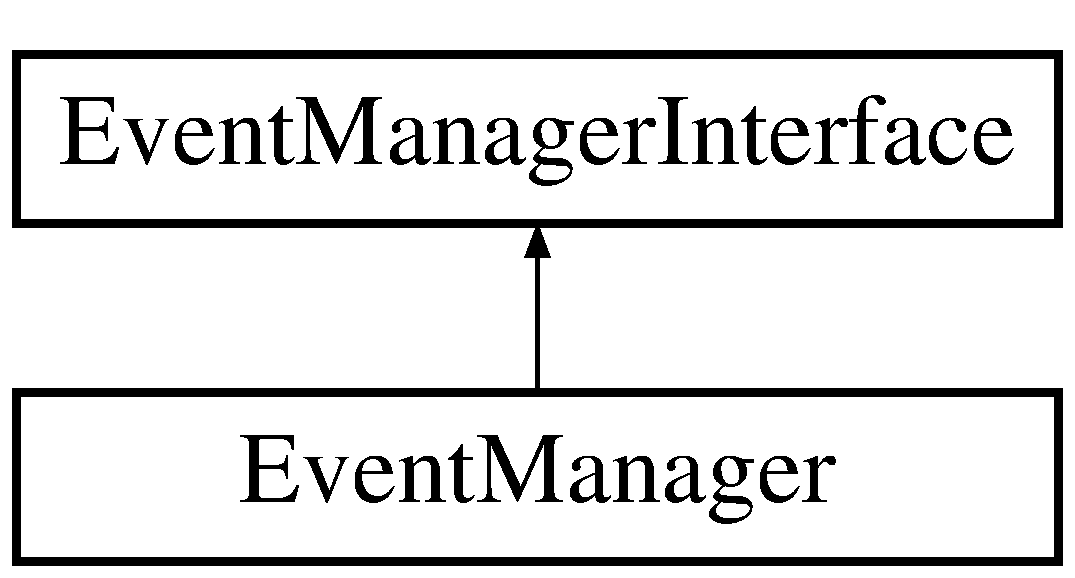
\includegraphics[height=2.000000cm]{classEventManagerInterface}
\end{center}
\end{figure}
\subsection*{Public Member Functions}
\begin{DoxyCompactItemize}
\item 
virtual \hyperlink{classEventManagerInterface_a257aedebff89184f009051dc2b29681f}{$\sim$\-Event\-Manager\-Interface} ()
\item 
virtual void \hyperlink{classEventManagerInterface_a13e851b9fa61887ab99dc0bba907bd05}{initialise} (\hyperlink{classGameEngineInterface}{Game\-Engine\-Interface} $\ast$engine)=0
\item 
virtual void \hyperlink{classEventManagerInterface_ad200ac2b9ee453cc3c954199e79f903d}{register\-Handler} (\hyperlink{classGameSystemInterface}{Game\-System\-Interface} $\ast$system)=0
\item 
virtual void \hyperlink{classEventManagerInterface_acaf7d1c9783158264d756c51f8d933fc}{raise\-Event} (\hyperlink{classEvent}{Event} $\ast$event)=0
\item 
virtual void \hyperlink{classEventManagerInterface_a4c8fb510a0ada3125e798c8d584b6e5f}{process\-Events} ()=0
\end{DoxyCompactItemize}


\subsection{Constructor \& Destructor Documentation}
\hypertarget{classEventManagerInterface_a257aedebff89184f009051dc2b29681f}{\index{Event\-Manager\-Interface@{Event\-Manager\-Interface}!$\sim$\-Event\-Manager\-Interface@{$\sim$\-Event\-Manager\-Interface}}
\index{$\sim$\-Event\-Manager\-Interface@{$\sim$\-Event\-Manager\-Interface}!EventManagerInterface@{Event\-Manager\-Interface}}
\subsubsection[{$\sim$\-Event\-Manager\-Interface}]{\setlength{\rightskip}{0pt plus 5cm}virtual Event\-Manager\-Interface\-::$\sim$\-Event\-Manager\-Interface (
\begin{DoxyParamCaption}
{}
\end{DoxyParamCaption}
)\hspace{0.3cm}{\ttfamily [inline]}, {\ttfamily [virtual]}}}\label{classEventManagerInterface_a257aedebff89184f009051dc2b29681f}


\subsection{Member Function Documentation}
\hypertarget{classEventManagerInterface_a13e851b9fa61887ab99dc0bba907bd05}{\index{Event\-Manager\-Interface@{Event\-Manager\-Interface}!initialise@{initialise}}
\index{initialise@{initialise}!EventManagerInterface@{Event\-Manager\-Interface}}
\subsubsection[{initialise}]{\setlength{\rightskip}{0pt plus 5cm}virtual void Event\-Manager\-Interface\-::initialise (
\begin{DoxyParamCaption}
\item[{{\bf Game\-Engine\-Interface} $\ast$}]{engine}
\end{DoxyParamCaption}
)\hspace{0.3cm}{\ttfamily [pure virtual]}}}\label{classEventManagerInterface_a13e851b9fa61887ab99dc0bba907bd05}


Implemented in \hyperlink{classEventManager_a93b64a8bc38a9842d10ee1526016671f}{Event\-Manager}.

\hypertarget{classEventManagerInterface_a4c8fb510a0ada3125e798c8d584b6e5f}{\index{Event\-Manager\-Interface@{Event\-Manager\-Interface}!process\-Events@{process\-Events}}
\index{process\-Events@{process\-Events}!EventManagerInterface@{Event\-Manager\-Interface}}
\subsubsection[{process\-Events}]{\setlength{\rightskip}{0pt plus 5cm}virtual void Event\-Manager\-Interface\-::process\-Events (
\begin{DoxyParamCaption}
{}
\end{DoxyParamCaption}
)\hspace{0.3cm}{\ttfamily [pure virtual]}}}\label{classEventManagerInterface_a4c8fb510a0ada3125e798c8d584b6e5f}


Implemented in \hyperlink{classEventManager_ad40f65674444d1944159dd85888740d3}{Event\-Manager}.

\hypertarget{classEventManagerInterface_acaf7d1c9783158264d756c51f8d933fc}{\index{Event\-Manager\-Interface@{Event\-Manager\-Interface}!raise\-Event@{raise\-Event}}
\index{raise\-Event@{raise\-Event}!EventManagerInterface@{Event\-Manager\-Interface}}
\subsubsection[{raise\-Event}]{\setlength{\rightskip}{0pt plus 5cm}virtual void Event\-Manager\-Interface\-::raise\-Event (
\begin{DoxyParamCaption}
\item[{{\bf Event} $\ast$}]{event}
\end{DoxyParamCaption}
)\hspace{0.3cm}{\ttfamily [pure virtual]}}}\label{classEventManagerInterface_acaf7d1c9783158264d756c51f8d933fc}


Implemented in \hyperlink{classEventManager_abce64060a5fb8cc3d51803b0d43f222f}{Event\-Manager}.

\hypertarget{classEventManagerInterface_ad200ac2b9ee453cc3c954199e79f903d}{\index{Event\-Manager\-Interface@{Event\-Manager\-Interface}!register\-Handler@{register\-Handler}}
\index{register\-Handler@{register\-Handler}!EventManagerInterface@{Event\-Manager\-Interface}}
\subsubsection[{register\-Handler}]{\setlength{\rightskip}{0pt plus 5cm}virtual void Event\-Manager\-Interface\-::register\-Handler (
\begin{DoxyParamCaption}
\item[{{\bf Game\-System\-Interface} $\ast$}]{system}
\end{DoxyParamCaption}
)\hspace{0.3cm}{\ttfamily [pure virtual]}}}\label{classEventManagerInterface_ad200ac2b9ee453cc3c954199e79f903d}


Implemented in \hyperlink{classEventManager_ae7c1bd23bc1beafa64b748553b471dce}{Event\-Manager}.



The documentation for this class was generated from the following file\-:\begin{DoxyCompactItemize}
\item 
\hyperlink{event__manager__interface_8h}{event\-\_\-manager\-\_\-interface.\-h}\end{DoxyCompactItemize}

\hypertarget{classGameEngine}{\section{Game\-Engine Class Reference}
\label{classGameEngine}\index{Game\-Engine@{Game\-Engine}}
}


{\ttfamily \#include $<$gameengine.\-h$>$}

Inheritance diagram for Game\-Engine\-:\begin{figure}[H]
\begin{center}
\leavevmode
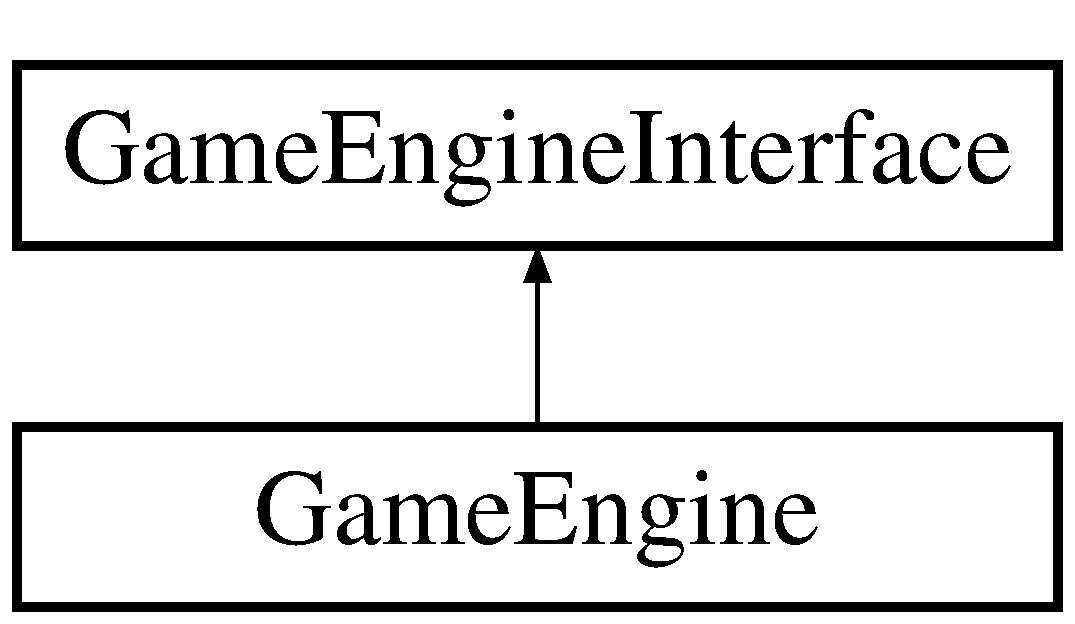
\includegraphics[height=2.000000cm]{classGameEngine}
\end{center}
\end{figure}
\subsection*{Public Member Functions}
\begin{DoxyCompactItemize}
\item 
\hyperlink{classGameEngine_a24a61ae50e4acd529abf6db0e07a732b}{Game\-Engine} (\hyperlink{classGraphicsInterface}{Graphics\-Interface} $\ast$a\-\_\-graphics)
\item 
\hyperlink{classGameEngine_a8e59d8341ef9d2dcc62eee1437e37f14}{$\sim$\-Game\-Engine} ()
\item 
void \hyperlink{classGameEngine_a6b4efc1f1d83f8c54c9f51f083705b81}{initialise} (void)
\item 
void \hyperlink{classGameEngine_a1df5865f2b074ef0fc68e6438b2fa265}{tick} (void)
\item 
void \hyperlink{classGameEngine_ad82b626def2e52b28f0d6c2d167589f6}{quit} ()
\item 
bool \hyperlink{classGameEngine_a789635fa84c65458455506ef54285b19}{is\-Player\-Turn} ()
\item 
void \hyperlink{classGameEngine_aa6181abb92ead7a904649fa03742caab}{swap\-Turn} ()
\item 
void \hyperlink{classGameEngine_af8db59fc46f510d9f6fd93c129b32a30}{raise\-Event} (\hyperlink{classEvent}{Event} $\ast$event)
\item 
\hyperlink{classEntityManagerInterface}{Entity\-Manager\-Interface} $\ast$ \hyperlink{classGameEngine_abb290b49ef61faec60a4960ac9df4303}{get\-Entities} ()
\item 
void \hyperlink{classGameEngine_a6116c0b6acf3ed29b7020f1df9b69403}{load\-Map} (const std\-::string \&map\-Name)
\item 
unsigned long long \hyperlink{classGameEngine_a0be043b34ca2bae3734e025f9d3f0bf0}{get\-Tick} ()
\item 
\hyperlink{classWindowManagerInterface}{Window\-Manager\-Interface} $\ast$ \hyperlink{classGameEngine_a28923eb5e29aac5f9541ca4af1ed17c3}{get\-Windows} ()
\item 
\hyperlink{classGraphicsInterface}{Graphics\-Interface} $\ast$ \hyperlink{classGameEngine_a602659da54f2d3fd5f3df555d22da2bc}{get\-Graphics} ()
\item 
void \hyperlink{classGameEngine_a014c9925928164befd6aa03d6bc21dbc}{set\-Entity\-Manager} (\hyperlink{classEntityManagerInterface}{Entity\-Manager\-Interface} $\ast$a\-\_\-manager)
\item 
void \hyperlink{classGameEngine_a27773808b06416c54beb52069c966a3b}{set\-Window\-Manager} (\hyperlink{classWindowManagerInterface}{Window\-Manager\-Interface} $\ast$a\-\_\-manager)
\item 
void \hyperlink{classGameEngine_a106e8e5d663134be9269b1a94b166c4a}{set\-Event\-Manager} (\hyperlink{classEventManagerInterface}{Event\-Manager\-Interface} $\ast$a\-\_\-manager)
\item 
void \hyperlink{classGameEngine_a58c80c2beb150f2816112371476aee12}{add\-System} (\hyperlink{classGameSystemInterface}{Game\-System\-Interface} $\ast$a\-\_\-system)
\item 
void \hyperlink{classGameEngine_a35bcdcd4574b2b1148fcff5a46a9277d}{set\-Generator} (\hyperlink{classGeneratorInterface}{Generator\-Interface} $\ast$a\-\_\-generator)
\end{DoxyCompactItemize}
\subsection*{Private Attributes}
\begin{DoxyCompactItemize}
\item 
unsigned long long \hyperlink{classGameEngine_ae50a77cf15fb12d6bb3e70ea64d4e652}{m\-\_\-tick}
\item 
bool \hyperlink{classGameEngine_af947cd69a795991a32716391175f61bc}{m\-\_\-player\-Turn}
\item 
\hyperlink{classEntityManagerInterface}{Entity\-Manager\-Interface} $\ast$ \hyperlink{classGameEngine_a3bf658348acbe7dafc657dc9c5442102}{m\-\_\-entity\-Manager}
\item 
\hyperlink{classEventManagerInterface}{Event\-Manager\-Interface} $\ast$ \hyperlink{classGameEngine_ab6c16baef2f287aef03cb336c831cdf6}{m\-\_\-event\-Manager}
\item 
\hyperlink{classWindowManagerInterface}{Window\-Manager\-Interface} $\ast$ \hyperlink{classGameEngine_a3308c8793731727773dbbd4614e06db6}{m\-\_\-window\-Manager}
\item 
std\-::vector\\*
$<$ \hyperlink{classGameSystemInterface}{Game\-System\-Interface} $\ast$ $>$ \hyperlink{classGameEngine_acc3e703e0019b3a5920a2d01339ccd68}{m\-\_\-systems}
\item 
\hyperlink{classGraphicsInterface}{Graphics\-Interface} $\ast$ \hyperlink{classGameEngine_a622586460faf2b46676aee1918d6a7eb}{m\-\_\-graphics}
\item 
\hyperlink{classGeneratorInterface}{Generator\-Interface} $\ast$ \hyperlink{classGameEngine_a8ce4a186b42c05555660321ae72efe9c}{m\-\_\-generator}
\end{DoxyCompactItemize}


\subsection{Constructor \& Destructor Documentation}
\hypertarget{classGameEngine_a24a61ae50e4acd529abf6db0e07a732b}{\index{Game\-Engine@{Game\-Engine}!Game\-Engine@{Game\-Engine}}
\index{Game\-Engine@{Game\-Engine}!GameEngine@{Game\-Engine}}
\subsubsection[{Game\-Engine}]{\setlength{\rightskip}{0pt plus 5cm}Game\-Engine\-::\-Game\-Engine (
\begin{DoxyParamCaption}
\item[{{\bf Graphics\-Interface} $\ast$}]{a\-\_\-graphics}
\end{DoxyParamCaption}
)}}\label{classGameEngine_a24a61ae50e4acd529abf6db0e07a732b}
\hypertarget{classGameEngine_a8e59d8341ef9d2dcc62eee1437e37f14}{\index{Game\-Engine@{Game\-Engine}!$\sim$\-Game\-Engine@{$\sim$\-Game\-Engine}}
\index{$\sim$\-Game\-Engine@{$\sim$\-Game\-Engine}!GameEngine@{Game\-Engine}}
\subsubsection[{$\sim$\-Game\-Engine}]{\setlength{\rightskip}{0pt plus 5cm}Game\-Engine\-::$\sim$\-Game\-Engine (
\begin{DoxyParamCaption}
{}
\end{DoxyParamCaption}
)}}\label{classGameEngine_a8e59d8341ef9d2dcc62eee1437e37f14}


\subsection{Member Function Documentation}
\hypertarget{classGameEngine_a58c80c2beb150f2816112371476aee12}{\index{Game\-Engine@{Game\-Engine}!add\-System@{add\-System}}
\index{add\-System@{add\-System}!GameEngine@{Game\-Engine}}
\subsubsection[{add\-System}]{\setlength{\rightskip}{0pt plus 5cm}void Game\-Engine\-::add\-System (
\begin{DoxyParamCaption}
\item[{{\bf Game\-System\-Interface} $\ast$}]{a\-\_\-system}
\end{DoxyParamCaption}
)\hspace{0.3cm}{\ttfamily [inline]}}}\label{classGameEngine_a58c80c2beb150f2816112371476aee12}
\hypertarget{classGameEngine_abb290b49ef61faec60a4960ac9df4303}{\index{Game\-Engine@{Game\-Engine}!get\-Entities@{get\-Entities}}
\index{get\-Entities@{get\-Entities}!GameEngine@{Game\-Engine}}
\subsubsection[{get\-Entities}]{\setlength{\rightskip}{0pt plus 5cm}{\bf Entity\-Manager\-Interface}$\ast$ Game\-Engine\-::get\-Entities (
\begin{DoxyParamCaption}
{}
\end{DoxyParamCaption}
)\hspace{0.3cm}{\ttfamily [inline]}, {\ttfamily [virtual]}}}\label{classGameEngine_abb290b49ef61faec60a4960ac9df4303}


Implements \hyperlink{classGameEngineInterface_ac7b9bb5c99fd8fec773a64d492d1869e}{Game\-Engine\-Interface}.

\hypertarget{classGameEngine_a602659da54f2d3fd5f3df555d22da2bc}{\index{Game\-Engine@{Game\-Engine}!get\-Graphics@{get\-Graphics}}
\index{get\-Graphics@{get\-Graphics}!GameEngine@{Game\-Engine}}
\subsubsection[{get\-Graphics}]{\setlength{\rightskip}{0pt plus 5cm}{\bf Graphics\-Interface}$\ast$ Game\-Engine\-::get\-Graphics (
\begin{DoxyParamCaption}
{}
\end{DoxyParamCaption}
)\hspace{0.3cm}{\ttfamily [inline]}, {\ttfamily [virtual]}}}\label{classGameEngine_a602659da54f2d3fd5f3df555d22da2bc}


Implements \hyperlink{classGameEngineInterface_ad1f1c9ed5b4e809c1133719af535db2d}{Game\-Engine\-Interface}.

\hypertarget{classGameEngine_a0be043b34ca2bae3734e025f9d3f0bf0}{\index{Game\-Engine@{Game\-Engine}!get\-Tick@{get\-Tick}}
\index{get\-Tick@{get\-Tick}!GameEngine@{Game\-Engine}}
\subsubsection[{get\-Tick}]{\setlength{\rightskip}{0pt plus 5cm}unsigned long long Game\-Engine\-::get\-Tick (
\begin{DoxyParamCaption}
{}
\end{DoxyParamCaption}
)\hspace{0.3cm}{\ttfamily [inline]}, {\ttfamily [virtual]}}}\label{classGameEngine_a0be043b34ca2bae3734e025f9d3f0bf0}


Implements \hyperlink{classGameEngineInterface_adcdcb9774de6e2df6ef0d0c45f3216d7}{Game\-Engine\-Interface}.

\hypertarget{classGameEngine_a28923eb5e29aac5f9541ca4af1ed17c3}{\index{Game\-Engine@{Game\-Engine}!get\-Windows@{get\-Windows}}
\index{get\-Windows@{get\-Windows}!GameEngine@{Game\-Engine}}
\subsubsection[{get\-Windows}]{\setlength{\rightskip}{0pt plus 5cm}{\bf Window\-Manager\-Interface}$\ast$ Game\-Engine\-::get\-Windows (
\begin{DoxyParamCaption}
{}
\end{DoxyParamCaption}
)\hspace{0.3cm}{\ttfamily [inline]}, {\ttfamily [virtual]}}}\label{classGameEngine_a28923eb5e29aac5f9541ca4af1ed17c3}


Implements \hyperlink{classGameEngineInterface_a2c99c33358dd5c5a34e046887440ced1}{Game\-Engine\-Interface}.

\hypertarget{classGameEngine_a6b4efc1f1d83f8c54c9f51f083705b81}{\index{Game\-Engine@{Game\-Engine}!initialise@{initialise}}
\index{initialise@{initialise}!GameEngine@{Game\-Engine}}
\subsubsection[{initialise}]{\setlength{\rightskip}{0pt plus 5cm}void Game\-Engine\-::initialise (
\begin{DoxyParamCaption}
\item[{void}]{}
\end{DoxyParamCaption}
)\hspace{0.3cm}{\ttfamily [virtual]}}}\label{classGameEngine_a6b4efc1f1d83f8c54c9f51f083705b81}


Implements \hyperlink{classGameEngineInterface_a25d6afec02af24ef82961dc32deee5d3}{Game\-Engine\-Interface}.

\hypertarget{classGameEngine_a789635fa84c65458455506ef54285b19}{\index{Game\-Engine@{Game\-Engine}!is\-Player\-Turn@{is\-Player\-Turn}}
\index{is\-Player\-Turn@{is\-Player\-Turn}!GameEngine@{Game\-Engine}}
\subsubsection[{is\-Player\-Turn}]{\setlength{\rightskip}{0pt plus 5cm}bool Game\-Engine\-::is\-Player\-Turn (
\begin{DoxyParamCaption}
{}
\end{DoxyParamCaption}
)\hspace{0.3cm}{\ttfamily [inline]}, {\ttfamily [virtual]}}}\label{classGameEngine_a789635fa84c65458455506ef54285b19}


Implements \hyperlink{classGameEngineInterface_a1f8c96fabf08e5f978859611a68eab03}{Game\-Engine\-Interface}.

\hypertarget{classGameEngine_a6116c0b6acf3ed29b7020f1df9b69403}{\index{Game\-Engine@{Game\-Engine}!load\-Map@{load\-Map}}
\index{load\-Map@{load\-Map}!GameEngine@{Game\-Engine}}
\subsubsection[{load\-Map}]{\setlength{\rightskip}{0pt plus 5cm}void Game\-Engine\-::load\-Map (
\begin{DoxyParamCaption}
\item[{const std\-::string \&}]{map\-Name}
\end{DoxyParamCaption}
)\hspace{0.3cm}{\ttfamily [virtual]}}}\label{classGameEngine_a6116c0b6acf3ed29b7020f1df9b69403}


Implements \hyperlink{classGameEngineInterface_aa7dc3bc46f821ac6f545f191272be2b3}{Game\-Engine\-Interface}.

\hypertarget{classGameEngine_ad82b626def2e52b28f0d6c2d167589f6}{\index{Game\-Engine@{Game\-Engine}!quit@{quit}}
\index{quit@{quit}!GameEngine@{Game\-Engine}}
\subsubsection[{quit}]{\setlength{\rightskip}{0pt plus 5cm}void Game\-Engine\-::quit (
\begin{DoxyParamCaption}
{}
\end{DoxyParamCaption}
)\hspace{0.3cm}{\ttfamily [inline]}, {\ttfamily [virtual]}}}\label{classGameEngine_ad82b626def2e52b28f0d6c2d167589f6}


Implements \hyperlink{classGameEngineInterface_a835c89ce5e9dac696f2b776e8b3fd6db}{Game\-Engine\-Interface}.

\hypertarget{classGameEngine_af8db59fc46f510d9f6fd93c129b32a30}{\index{Game\-Engine@{Game\-Engine}!raise\-Event@{raise\-Event}}
\index{raise\-Event@{raise\-Event}!GameEngine@{Game\-Engine}}
\subsubsection[{raise\-Event}]{\setlength{\rightskip}{0pt plus 5cm}void Game\-Engine\-::raise\-Event (
\begin{DoxyParamCaption}
\item[{{\bf Event} $\ast$}]{event}
\end{DoxyParamCaption}
)\hspace{0.3cm}{\ttfamily [inline]}, {\ttfamily [virtual]}}}\label{classGameEngine_af8db59fc46f510d9f6fd93c129b32a30}


Implements \hyperlink{classGameEngineInterface_a4826bce0dc77598e2ca0869ce2462db7}{Game\-Engine\-Interface}.

\hypertarget{classGameEngine_a014c9925928164befd6aa03d6bc21dbc}{\index{Game\-Engine@{Game\-Engine}!set\-Entity\-Manager@{set\-Entity\-Manager}}
\index{set\-Entity\-Manager@{set\-Entity\-Manager}!GameEngine@{Game\-Engine}}
\subsubsection[{set\-Entity\-Manager}]{\setlength{\rightskip}{0pt plus 5cm}void Game\-Engine\-::set\-Entity\-Manager (
\begin{DoxyParamCaption}
\item[{{\bf Entity\-Manager\-Interface} $\ast$}]{a\-\_\-manager}
\end{DoxyParamCaption}
)\hspace{0.3cm}{\ttfamily [inline]}}}\label{classGameEngine_a014c9925928164befd6aa03d6bc21dbc}
\hypertarget{classGameEngine_a106e8e5d663134be9269b1a94b166c4a}{\index{Game\-Engine@{Game\-Engine}!set\-Event\-Manager@{set\-Event\-Manager}}
\index{set\-Event\-Manager@{set\-Event\-Manager}!GameEngine@{Game\-Engine}}
\subsubsection[{set\-Event\-Manager}]{\setlength{\rightskip}{0pt plus 5cm}void Game\-Engine\-::set\-Event\-Manager (
\begin{DoxyParamCaption}
\item[{{\bf Event\-Manager\-Interface} $\ast$}]{a\-\_\-manager}
\end{DoxyParamCaption}
)\hspace{0.3cm}{\ttfamily [inline]}}}\label{classGameEngine_a106e8e5d663134be9269b1a94b166c4a}
\hypertarget{classGameEngine_a35bcdcd4574b2b1148fcff5a46a9277d}{\index{Game\-Engine@{Game\-Engine}!set\-Generator@{set\-Generator}}
\index{set\-Generator@{set\-Generator}!GameEngine@{Game\-Engine}}
\subsubsection[{set\-Generator}]{\setlength{\rightskip}{0pt plus 5cm}void Game\-Engine\-::set\-Generator (
\begin{DoxyParamCaption}
\item[{{\bf Generator\-Interface} $\ast$}]{a\-\_\-generator}
\end{DoxyParamCaption}
)\hspace{0.3cm}{\ttfamily [inline]}}}\label{classGameEngine_a35bcdcd4574b2b1148fcff5a46a9277d}
\hypertarget{classGameEngine_a27773808b06416c54beb52069c966a3b}{\index{Game\-Engine@{Game\-Engine}!set\-Window\-Manager@{set\-Window\-Manager}}
\index{set\-Window\-Manager@{set\-Window\-Manager}!GameEngine@{Game\-Engine}}
\subsubsection[{set\-Window\-Manager}]{\setlength{\rightskip}{0pt plus 5cm}void Game\-Engine\-::set\-Window\-Manager (
\begin{DoxyParamCaption}
\item[{{\bf Window\-Manager\-Interface} $\ast$}]{a\-\_\-manager}
\end{DoxyParamCaption}
)\hspace{0.3cm}{\ttfamily [inline]}}}\label{classGameEngine_a27773808b06416c54beb52069c966a3b}
\hypertarget{classGameEngine_aa6181abb92ead7a904649fa03742caab}{\index{Game\-Engine@{Game\-Engine}!swap\-Turn@{swap\-Turn}}
\index{swap\-Turn@{swap\-Turn}!GameEngine@{Game\-Engine}}
\subsubsection[{swap\-Turn}]{\setlength{\rightskip}{0pt plus 5cm}void Game\-Engine\-::swap\-Turn (
\begin{DoxyParamCaption}
{}
\end{DoxyParamCaption}
)\hspace{0.3cm}{\ttfamily [inline]}, {\ttfamily [virtual]}}}\label{classGameEngine_aa6181abb92ead7a904649fa03742caab}


Implements \hyperlink{classGameEngineInterface_aff6fe7a94c1421f26642cf0485c2d4ce}{Game\-Engine\-Interface}.

\hypertarget{classGameEngine_a1df5865f2b074ef0fc68e6438b2fa265}{\index{Game\-Engine@{Game\-Engine}!tick@{tick}}
\index{tick@{tick}!GameEngine@{Game\-Engine}}
\subsubsection[{tick}]{\setlength{\rightskip}{0pt plus 5cm}void Game\-Engine\-::tick (
\begin{DoxyParamCaption}
\item[{void}]{}
\end{DoxyParamCaption}
)\hspace{0.3cm}{\ttfamily [virtual]}}}\label{classGameEngine_a1df5865f2b074ef0fc68e6438b2fa265}


Implements \hyperlink{classGameEngineInterface_a018db9a3868f8ef3c5b864bae5047a42}{Game\-Engine\-Interface}.



\subsection{Member Data Documentation}
\hypertarget{classGameEngine_a3bf658348acbe7dafc657dc9c5442102}{\index{Game\-Engine@{Game\-Engine}!m\-\_\-entity\-Manager@{m\-\_\-entity\-Manager}}
\index{m\-\_\-entity\-Manager@{m\-\_\-entity\-Manager}!GameEngine@{Game\-Engine}}
\subsubsection[{m\-\_\-entity\-Manager}]{\setlength{\rightskip}{0pt plus 5cm}{\bf Entity\-Manager\-Interface}$\ast$ Game\-Engine\-::m\-\_\-entity\-Manager\hspace{0.3cm}{\ttfamily [private]}}}\label{classGameEngine_a3bf658348acbe7dafc657dc9c5442102}
\hypertarget{classGameEngine_ab6c16baef2f287aef03cb336c831cdf6}{\index{Game\-Engine@{Game\-Engine}!m\-\_\-event\-Manager@{m\-\_\-event\-Manager}}
\index{m\-\_\-event\-Manager@{m\-\_\-event\-Manager}!GameEngine@{Game\-Engine}}
\subsubsection[{m\-\_\-event\-Manager}]{\setlength{\rightskip}{0pt plus 5cm}{\bf Event\-Manager\-Interface}$\ast$ Game\-Engine\-::m\-\_\-event\-Manager\hspace{0.3cm}{\ttfamily [private]}}}\label{classGameEngine_ab6c16baef2f287aef03cb336c831cdf6}
\hypertarget{classGameEngine_a8ce4a186b42c05555660321ae72efe9c}{\index{Game\-Engine@{Game\-Engine}!m\-\_\-generator@{m\-\_\-generator}}
\index{m\-\_\-generator@{m\-\_\-generator}!GameEngine@{Game\-Engine}}
\subsubsection[{m\-\_\-generator}]{\setlength{\rightskip}{0pt plus 5cm}{\bf Generator\-Interface}$\ast$ Game\-Engine\-::m\-\_\-generator\hspace{0.3cm}{\ttfamily [private]}}}\label{classGameEngine_a8ce4a186b42c05555660321ae72efe9c}
\hypertarget{classGameEngine_a622586460faf2b46676aee1918d6a7eb}{\index{Game\-Engine@{Game\-Engine}!m\-\_\-graphics@{m\-\_\-graphics}}
\index{m\-\_\-graphics@{m\-\_\-graphics}!GameEngine@{Game\-Engine}}
\subsubsection[{m\-\_\-graphics}]{\setlength{\rightskip}{0pt plus 5cm}{\bf Graphics\-Interface}$\ast$ Game\-Engine\-::m\-\_\-graphics\hspace{0.3cm}{\ttfamily [private]}}}\label{classGameEngine_a622586460faf2b46676aee1918d6a7eb}
\hypertarget{classGameEngine_af947cd69a795991a32716391175f61bc}{\index{Game\-Engine@{Game\-Engine}!m\-\_\-player\-Turn@{m\-\_\-player\-Turn}}
\index{m\-\_\-player\-Turn@{m\-\_\-player\-Turn}!GameEngine@{Game\-Engine}}
\subsubsection[{m\-\_\-player\-Turn}]{\setlength{\rightskip}{0pt plus 5cm}bool Game\-Engine\-::m\-\_\-player\-Turn\hspace{0.3cm}{\ttfamily [private]}}}\label{classGameEngine_af947cd69a795991a32716391175f61bc}
\hypertarget{classGameEngine_acc3e703e0019b3a5920a2d01339ccd68}{\index{Game\-Engine@{Game\-Engine}!m\-\_\-systems@{m\-\_\-systems}}
\index{m\-\_\-systems@{m\-\_\-systems}!GameEngine@{Game\-Engine}}
\subsubsection[{m\-\_\-systems}]{\setlength{\rightskip}{0pt plus 5cm}std\-::vector$<${\bf Game\-System\-Interface}$\ast$$>$ Game\-Engine\-::m\-\_\-systems\hspace{0.3cm}{\ttfamily [private]}}}\label{classGameEngine_acc3e703e0019b3a5920a2d01339ccd68}
\hypertarget{classGameEngine_ae50a77cf15fb12d6bb3e70ea64d4e652}{\index{Game\-Engine@{Game\-Engine}!m\-\_\-tick@{m\-\_\-tick}}
\index{m\-\_\-tick@{m\-\_\-tick}!GameEngine@{Game\-Engine}}
\subsubsection[{m\-\_\-tick}]{\setlength{\rightskip}{0pt plus 5cm}unsigned long long Game\-Engine\-::m\-\_\-tick\hspace{0.3cm}{\ttfamily [private]}}}\label{classGameEngine_ae50a77cf15fb12d6bb3e70ea64d4e652}
\hypertarget{classGameEngine_a3308c8793731727773dbbd4614e06db6}{\index{Game\-Engine@{Game\-Engine}!m\-\_\-window\-Manager@{m\-\_\-window\-Manager}}
\index{m\-\_\-window\-Manager@{m\-\_\-window\-Manager}!GameEngine@{Game\-Engine}}
\subsubsection[{m\-\_\-window\-Manager}]{\setlength{\rightskip}{0pt plus 5cm}{\bf Window\-Manager\-Interface}$\ast$ Game\-Engine\-::m\-\_\-window\-Manager\hspace{0.3cm}{\ttfamily [private]}}}\label{classGameEngine_a3308c8793731727773dbbd4614e06db6}


The documentation for this class was generated from the following files\-:\begin{DoxyCompactItemize}
\item 
\hyperlink{gameengine_8h}{gameengine.\-h}\item 
\hyperlink{gameengine_8cpp}{gameengine.\-cpp}\end{DoxyCompactItemize}

\hypertarget{classGameEngineInterface}{\section{Game\-Engine\-Interface Class Reference}
\label{classGameEngineInterface}\index{Game\-Engine\-Interface@{Game\-Engine\-Interface}}
}


{\ttfamily \#include $<$game\-\_\-engine\-\_\-interface.\-h$>$}

Inheritance diagram for Game\-Engine\-Interface\-:\begin{figure}[H]
\begin{center}
\leavevmode
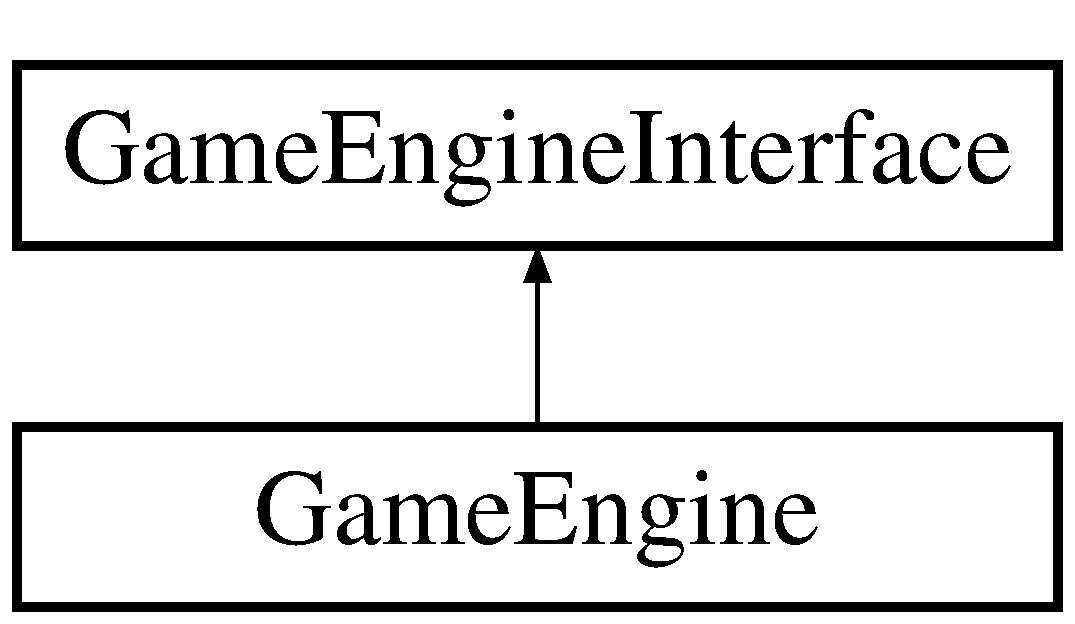
\includegraphics[height=2.000000cm]{classGameEngineInterface}
\end{center}
\end{figure}
\subsection*{Public Member Functions}
\begin{DoxyCompactItemize}
\item 
\hyperlink{classGameEngineInterface_acfe04e158f13c49fa34201d965856f98}{Game\-Engine\-Interface} ()
\item 
virtual \hyperlink{classGameEngineInterface_a3f62425d6da8aa68ee3698dc3034aa89}{$\sim$\-Game\-Engine\-Interface} ()
\item 
virtual void \hyperlink{classGameEngineInterface_a25d6afec02af24ef82961dc32deee5d3}{initialise} (void)=0
\item 
virtual void \hyperlink{classGameEngineInterface_a018db9a3868f8ef3c5b864bae5047a42}{tick} (void)=0
\item 
virtual void \hyperlink{classGameEngineInterface_a835c89ce5e9dac696f2b776e8b3fd6db}{quit} ()=0
\item 
virtual bool \hyperlink{classGameEngineInterface_a1f8c96fabf08e5f978859611a68eab03}{is\-Player\-Turn} ()=0
\item 
virtual void \hyperlink{classGameEngineInterface_aff6fe7a94c1421f26642cf0485c2d4ce}{swap\-Turn} ()=0
\item 
virtual void \hyperlink{classGameEngineInterface_a4826bce0dc77598e2ca0869ce2462db7}{raise\-Event} (\hyperlink{classEvent}{Event} $\ast$event)=0
\item 
virtual \hyperlink{classEntityManagerInterface}{Entity\-Manager\-Interface} $\ast$ \hyperlink{classGameEngineInterface_ac7b9bb5c99fd8fec773a64d492d1869e}{get\-Entities} ()=0
\item 
virtual void \hyperlink{classGameEngineInterface_aa7dc3bc46f821ac6f545f191272be2b3}{load\-Map} (const std\-::string \&map\-Name)=0
\item 
virtual unsigned long long \hyperlink{classGameEngineInterface_adcdcb9774de6e2df6ef0d0c45f3216d7}{get\-Tick} ()=0
\item 
virtual \hyperlink{classWindowManagerInterface}{Window\-Manager\-Interface} $\ast$ \hyperlink{classGameEngineInterface_a2c99c33358dd5c5a34e046887440ced1}{get\-Windows} ()=0
\item 
virtual \hyperlink{classGraphicsInterface}{Graphics\-Interface} $\ast$ \hyperlink{classGameEngineInterface_ad1f1c9ed5b4e809c1133719af535db2d}{get\-Graphics} ()=0
\end{DoxyCompactItemize}


\subsection{Constructor \& Destructor Documentation}
\hypertarget{classGameEngineInterface_acfe04e158f13c49fa34201d965856f98}{\index{Game\-Engine\-Interface@{Game\-Engine\-Interface}!Game\-Engine\-Interface@{Game\-Engine\-Interface}}
\index{Game\-Engine\-Interface@{Game\-Engine\-Interface}!GameEngineInterface@{Game\-Engine\-Interface}}
\subsubsection[{Game\-Engine\-Interface}]{\setlength{\rightskip}{0pt plus 5cm}Game\-Engine\-Interface\-::\-Game\-Engine\-Interface (
\begin{DoxyParamCaption}
{}
\end{DoxyParamCaption}
)\hspace{0.3cm}{\ttfamily [inline]}}}\label{classGameEngineInterface_acfe04e158f13c49fa34201d965856f98}
\hypertarget{classGameEngineInterface_a3f62425d6da8aa68ee3698dc3034aa89}{\index{Game\-Engine\-Interface@{Game\-Engine\-Interface}!$\sim$\-Game\-Engine\-Interface@{$\sim$\-Game\-Engine\-Interface}}
\index{$\sim$\-Game\-Engine\-Interface@{$\sim$\-Game\-Engine\-Interface}!GameEngineInterface@{Game\-Engine\-Interface}}
\subsubsection[{$\sim$\-Game\-Engine\-Interface}]{\setlength{\rightskip}{0pt plus 5cm}virtual Game\-Engine\-Interface\-::$\sim$\-Game\-Engine\-Interface (
\begin{DoxyParamCaption}
{}
\end{DoxyParamCaption}
)\hspace{0.3cm}{\ttfamily [inline]}, {\ttfamily [virtual]}}}\label{classGameEngineInterface_a3f62425d6da8aa68ee3698dc3034aa89}


\subsection{Member Function Documentation}
\hypertarget{classGameEngineInterface_ac7b9bb5c99fd8fec773a64d492d1869e}{\index{Game\-Engine\-Interface@{Game\-Engine\-Interface}!get\-Entities@{get\-Entities}}
\index{get\-Entities@{get\-Entities}!GameEngineInterface@{Game\-Engine\-Interface}}
\subsubsection[{get\-Entities}]{\setlength{\rightskip}{0pt plus 5cm}virtual {\bf Entity\-Manager\-Interface}$\ast$ Game\-Engine\-Interface\-::get\-Entities (
\begin{DoxyParamCaption}
{}
\end{DoxyParamCaption}
)\hspace{0.3cm}{\ttfamily [pure virtual]}}}\label{classGameEngineInterface_ac7b9bb5c99fd8fec773a64d492d1869e}


Implemented in \hyperlink{classGameEngine_abb290b49ef61faec60a4960ac9df4303}{Game\-Engine}.

\hypertarget{classGameEngineInterface_ad1f1c9ed5b4e809c1133719af535db2d}{\index{Game\-Engine\-Interface@{Game\-Engine\-Interface}!get\-Graphics@{get\-Graphics}}
\index{get\-Graphics@{get\-Graphics}!GameEngineInterface@{Game\-Engine\-Interface}}
\subsubsection[{get\-Graphics}]{\setlength{\rightskip}{0pt plus 5cm}virtual {\bf Graphics\-Interface}$\ast$ Game\-Engine\-Interface\-::get\-Graphics (
\begin{DoxyParamCaption}
{}
\end{DoxyParamCaption}
)\hspace{0.3cm}{\ttfamily [pure virtual]}}}\label{classGameEngineInterface_ad1f1c9ed5b4e809c1133719af535db2d}


Implemented in \hyperlink{classGameEngine_a602659da54f2d3fd5f3df555d22da2bc}{Game\-Engine}.

\hypertarget{classGameEngineInterface_adcdcb9774de6e2df6ef0d0c45f3216d7}{\index{Game\-Engine\-Interface@{Game\-Engine\-Interface}!get\-Tick@{get\-Tick}}
\index{get\-Tick@{get\-Tick}!GameEngineInterface@{Game\-Engine\-Interface}}
\subsubsection[{get\-Tick}]{\setlength{\rightskip}{0pt plus 5cm}virtual unsigned long long Game\-Engine\-Interface\-::get\-Tick (
\begin{DoxyParamCaption}
{}
\end{DoxyParamCaption}
)\hspace{0.3cm}{\ttfamily [pure virtual]}}}\label{classGameEngineInterface_adcdcb9774de6e2df6ef0d0c45f3216d7}


Implemented in \hyperlink{classGameEngine_a0be043b34ca2bae3734e025f9d3f0bf0}{Game\-Engine}.

\hypertarget{classGameEngineInterface_a2c99c33358dd5c5a34e046887440ced1}{\index{Game\-Engine\-Interface@{Game\-Engine\-Interface}!get\-Windows@{get\-Windows}}
\index{get\-Windows@{get\-Windows}!GameEngineInterface@{Game\-Engine\-Interface}}
\subsubsection[{get\-Windows}]{\setlength{\rightskip}{0pt plus 5cm}virtual {\bf Window\-Manager\-Interface}$\ast$ Game\-Engine\-Interface\-::get\-Windows (
\begin{DoxyParamCaption}
{}
\end{DoxyParamCaption}
)\hspace{0.3cm}{\ttfamily [pure virtual]}}}\label{classGameEngineInterface_a2c99c33358dd5c5a34e046887440ced1}


Implemented in \hyperlink{classGameEngine_a28923eb5e29aac5f9541ca4af1ed17c3}{Game\-Engine}.

\hypertarget{classGameEngineInterface_a25d6afec02af24ef82961dc32deee5d3}{\index{Game\-Engine\-Interface@{Game\-Engine\-Interface}!initialise@{initialise}}
\index{initialise@{initialise}!GameEngineInterface@{Game\-Engine\-Interface}}
\subsubsection[{initialise}]{\setlength{\rightskip}{0pt plus 5cm}virtual void Game\-Engine\-Interface\-::initialise (
\begin{DoxyParamCaption}
\item[{void}]{}
\end{DoxyParamCaption}
)\hspace{0.3cm}{\ttfamily [pure virtual]}}}\label{classGameEngineInterface_a25d6afec02af24ef82961dc32deee5d3}


Implemented in \hyperlink{classGameEngine_a6b4efc1f1d83f8c54c9f51f083705b81}{Game\-Engine}.

\hypertarget{classGameEngineInterface_a1f8c96fabf08e5f978859611a68eab03}{\index{Game\-Engine\-Interface@{Game\-Engine\-Interface}!is\-Player\-Turn@{is\-Player\-Turn}}
\index{is\-Player\-Turn@{is\-Player\-Turn}!GameEngineInterface@{Game\-Engine\-Interface}}
\subsubsection[{is\-Player\-Turn}]{\setlength{\rightskip}{0pt plus 5cm}virtual bool Game\-Engine\-Interface\-::is\-Player\-Turn (
\begin{DoxyParamCaption}
{}
\end{DoxyParamCaption}
)\hspace{0.3cm}{\ttfamily [pure virtual]}}}\label{classGameEngineInterface_a1f8c96fabf08e5f978859611a68eab03}


Implemented in \hyperlink{classGameEngine_a789635fa84c65458455506ef54285b19}{Game\-Engine}.

\hypertarget{classGameEngineInterface_aa7dc3bc46f821ac6f545f191272be2b3}{\index{Game\-Engine\-Interface@{Game\-Engine\-Interface}!load\-Map@{load\-Map}}
\index{load\-Map@{load\-Map}!GameEngineInterface@{Game\-Engine\-Interface}}
\subsubsection[{load\-Map}]{\setlength{\rightskip}{0pt plus 5cm}virtual void Game\-Engine\-Interface\-::load\-Map (
\begin{DoxyParamCaption}
\item[{const std\-::string \&}]{map\-Name}
\end{DoxyParamCaption}
)\hspace{0.3cm}{\ttfamily [pure virtual]}}}\label{classGameEngineInterface_aa7dc3bc46f821ac6f545f191272be2b3}


Implemented in \hyperlink{classGameEngine_a6116c0b6acf3ed29b7020f1df9b69403}{Game\-Engine}.

\hypertarget{classGameEngineInterface_a835c89ce5e9dac696f2b776e8b3fd6db}{\index{Game\-Engine\-Interface@{Game\-Engine\-Interface}!quit@{quit}}
\index{quit@{quit}!GameEngineInterface@{Game\-Engine\-Interface}}
\subsubsection[{quit}]{\setlength{\rightskip}{0pt plus 5cm}virtual void Game\-Engine\-Interface\-::quit (
\begin{DoxyParamCaption}
{}
\end{DoxyParamCaption}
)\hspace{0.3cm}{\ttfamily [pure virtual]}}}\label{classGameEngineInterface_a835c89ce5e9dac696f2b776e8b3fd6db}


Implemented in \hyperlink{classGameEngine_ad82b626def2e52b28f0d6c2d167589f6}{Game\-Engine}.

\hypertarget{classGameEngineInterface_a4826bce0dc77598e2ca0869ce2462db7}{\index{Game\-Engine\-Interface@{Game\-Engine\-Interface}!raise\-Event@{raise\-Event}}
\index{raise\-Event@{raise\-Event}!GameEngineInterface@{Game\-Engine\-Interface}}
\subsubsection[{raise\-Event}]{\setlength{\rightskip}{0pt plus 5cm}virtual void Game\-Engine\-Interface\-::raise\-Event (
\begin{DoxyParamCaption}
\item[{{\bf Event} $\ast$}]{event}
\end{DoxyParamCaption}
)\hspace{0.3cm}{\ttfamily [pure virtual]}}}\label{classGameEngineInterface_a4826bce0dc77598e2ca0869ce2462db7}


Implemented in \hyperlink{classGameEngine_af8db59fc46f510d9f6fd93c129b32a30}{Game\-Engine}.

\hypertarget{classGameEngineInterface_aff6fe7a94c1421f26642cf0485c2d4ce}{\index{Game\-Engine\-Interface@{Game\-Engine\-Interface}!swap\-Turn@{swap\-Turn}}
\index{swap\-Turn@{swap\-Turn}!GameEngineInterface@{Game\-Engine\-Interface}}
\subsubsection[{swap\-Turn}]{\setlength{\rightskip}{0pt plus 5cm}virtual void Game\-Engine\-Interface\-::swap\-Turn (
\begin{DoxyParamCaption}
{}
\end{DoxyParamCaption}
)\hspace{0.3cm}{\ttfamily [pure virtual]}}}\label{classGameEngineInterface_aff6fe7a94c1421f26642cf0485c2d4ce}


Implemented in \hyperlink{classGameEngine_aa6181abb92ead7a904649fa03742caab}{Game\-Engine}.

\hypertarget{classGameEngineInterface_a018db9a3868f8ef3c5b864bae5047a42}{\index{Game\-Engine\-Interface@{Game\-Engine\-Interface}!tick@{tick}}
\index{tick@{tick}!GameEngineInterface@{Game\-Engine\-Interface}}
\subsubsection[{tick}]{\setlength{\rightskip}{0pt plus 5cm}virtual void Game\-Engine\-Interface\-::tick (
\begin{DoxyParamCaption}
\item[{void}]{}
\end{DoxyParamCaption}
)\hspace{0.3cm}{\ttfamily [pure virtual]}}}\label{classGameEngineInterface_a018db9a3868f8ef3c5b864bae5047a42}


Implemented in \hyperlink{classGameEngine_a1df5865f2b074ef0fc68e6438b2fa265}{Game\-Engine}.



The documentation for this class was generated from the following file\-:\begin{DoxyCompactItemize}
\item 
\hyperlink{game__engine__interface_8h}{game\-\_\-engine\-\_\-interface.\-h}\end{DoxyCompactItemize}

\hypertarget{classGameSystemBase}{\section{Game\-System\-Base Class Reference}
\label{classGameSystemBase}\index{Game\-System\-Base@{Game\-System\-Base}}
}


{\ttfamily \#include $<$game\-\_\-system\-\_\-base.\-h$>$}

Inheritance diagram for Game\-System\-Base\-:\begin{figure}[H]
\begin{center}
\leavevmode
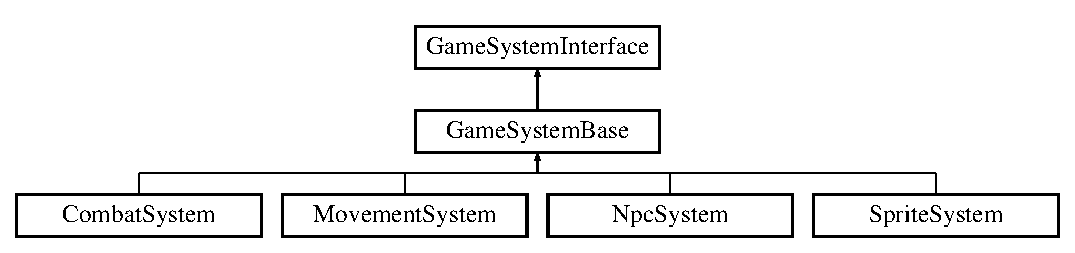
\includegraphics[height=2.957747cm]{classGameSystemBase}
\end{center}
\end{figure}
\subsection*{Public Member Functions}
\begin{DoxyCompactItemize}
\item 
\hyperlink{classGameSystemBase_a328ace5c41637f72e450083ce7159f66}{Game\-System\-Base} ()
\item 
virtual void \hyperlink{classGameSystemBase_a55b4fc27cbfccd3c724c2e5984d78625}{initialise} (\hyperlink{classGameEngineInterface}{Game\-Engine\-Interface} $\ast$engine)
\item 
virtual \hyperlink{classGameEngineInterface}{Game\-Engine\-Interface} $\ast$ \hyperlink{classGameSystemBase_a1954c5a1c79963554805bc25b2cd6072}{get\-Engine\-Ref} ()
\item 
virtual void \hyperlink{classGameSystemBase_a007b3ece290b1ad0dc3e397c5264d44d}{handle\-Event} (const \hyperlink{classEvent}{Event} $\ast$event)
\item 
virtual void \hyperlink{classGameSystemBase_a039d3086ac7fe50abdb110b569520d69}{update} ()
\item 
virtual \hyperlink{classGameSystemBase_a96f76df170673523b71d6c1dab8a7efd}{$\sim$\-Game\-System\-Base} ()
\item 
virtual std\-::vector$<$ \hyperlink{classEntity}{Entity} $\ast$ $>$ \hyperlink{classGameSystemBase_aae270a88f1077a091e6033514b889abd}{find\-Entities\-Near} (unsigned int x, unsigned int y, unsigned radius)
\item 
virtual std\-::vector$<$ \hyperlink{classEntity}{Entity} $\ast$ $>$ \hyperlink{classGameSystemBase_a7aa9912fc078d990dbfb480e411bd3bc}{find\-Entities\-At} (unsigned int x, unsigned int y)
\item 
virtual std\-::vector$<$ \hyperlink{classEntity}{Entity} $\ast$ $>$ \hyperlink{classGameSystemBase_a44456ef40ac565b9d6b65f3b1531a4ef}{find\-Entities\-To\-The} (\hyperlink{classMoveEntityEvent_a7058a943643bee9164a21e62e3392807}{Move\-Entity\-Event\-::\-D\-I\-R\-E\-C\-T\-I\-O\-N} a\-\_\-direction, \hyperlink{classEntity}{Entity} $\ast$a\-\_\-entity)
\end{DoxyCompactItemize}
\subsection*{Protected Attributes}
\begin{DoxyCompactItemize}
\item 
\hyperlink{classGameEngineInterface}{Game\-Engine\-Interface} $\ast$ \hyperlink{classGameSystemBase_aa9044eb22399f0c0ddd8f049738c62e5}{m\-\_\-engine}
\end{DoxyCompactItemize}


\subsection{Constructor \& Destructor Documentation}
\hypertarget{classGameSystemBase_a328ace5c41637f72e450083ce7159f66}{\index{Game\-System\-Base@{Game\-System\-Base}!Game\-System\-Base@{Game\-System\-Base}}
\index{Game\-System\-Base@{Game\-System\-Base}!GameSystemBase@{Game\-System\-Base}}
\subsubsection[{Game\-System\-Base}]{\setlength{\rightskip}{0pt plus 5cm}Game\-System\-Base\-::\-Game\-System\-Base (
\begin{DoxyParamCaption}
{}
\end{DoxyParamCaption}
)\hspace{0.3cm}{\ttfamily [inline]}}}\label{classGameSystemBase_a328ace5c41637f72e450083ce7159f66}
\hypertarget{classGameSystemBase_a96f76df170673523b71d6c1dab8a7efd}{\index{Game\-System\-Base@{Game\-System\-Base}!$\sim$\-Game\-System\-Base@{$\sim$\-Game\-System\-Base}}
\index{$\sim$\-Game\-System\-Base@{$\sim$\-Game\-System\-Base}!GameSystemBase@{Game\-System\-Base}}
\subsubsection[{$\sim$\-Game\-System\-Base}]{\setlength{\rightskip}{0pt plus 5cm}virtual Game\-System\-Base\-::$\sim$\-Game\-System\-Base (
\begin{DoxyParamCaption}
{}
\end{DoxyParamCaption}
)\hspace{0.3cm}{\ttfamily [inline]}, {\ttfamily [virtual]}}}\label{classGameSystemBase_a96f76df170673523b71d6c1dab8a7efd}


\subsection{Member Function Documentation}
\hypertarget{classGameSystemBase_a7aa9912fc078d990dbfb480e411bd3bc}{\index{Game\-System\-Base@{Game\-System\-Base}!find\-Entities\-At@{find\-Entities\-At}}
\index{find\-Entities\-At@{find\-Entities\-At}!GameSystemBase@{Game\-System\-Base}}
\subsubsection[{find\-Entities\-At}]{\setlength{\rightskip}{0pt plus 5cm}std\-::vector$<$ {\bf Entity} $\ast$ $>$ Game\-System\-Base\-::find\-Entities\-At (
\begin{DoxyParamCaption}
\item[{unsigned int}]{x, }
\item[{unsigned int}]{y}
\end{DoxyParamCaption}
)\hspace{0.3cm}{\ttfamily [virtual]}}}\label{classGameSystemBase_a7aa9912fc078d990dbfb480e411bd3bc}
\hypertarget{classGameSystemBase_aae270a88f1077a091e6033514b889abd}{\index{Game\-System\-Base@{Game\-System\-Base}!find\-Entities\-Near@{find\-Entities\-Near}}
\index{find\-Entities\-Near@{find\-Entities\-Near}!GameSystemBase@{Game\-System\-Base}}
\subsubsection[{find\-Entities\-Near}]{\setlength{\rightskip}{0pt plus 5cm}std\-::vector$<$ {\bf Entity} $\ast$ $>$ Game\-System\-Base\-::find\-Entities\-Near (
\begin{DoxyParamCaption}
\item[{unsigned int}]{x, }
\item[{unsigned int}]{y, }
\item[{unsigned}]{radius}
\end{DoxyParamCaption}
)\hspace{0.3cm}{\ttfamily [virtual]}}}\label{classGameSystemBase_aae270a88f1077a091e6033514b889abd}
\hypertarget{classGameSystemBase_a44456ef40ac565b9d6b65f3b1531a4ef}{\index{Game\-System\-Base@{Game\-System\-Base}!find\-Entities\-To\-The@{find\-Entities\-To\-The}}
\index{find\-Entities\-To\-The@{find\-Entities\-To\-The}!GameSystemBase@{Game\-System\-Base}}
\subsubsection[{find\-Entities\-To\-The}]{\setlength{\rightskip}{0pt plus 5cm}std\-::vector$<$ {\bf Entity} $\ast$ $>$ Game\-System\-Base\-::find\-Entities\-To\-The (
\begin{DoxyParamCaption}
\item[{{\bf Move\-Entity\-Event\-::\-D\-I\-R\-E\-C\-T\-I\-O\-N}}]{a\-\_\-direction, }
\item[{{\bf Entity} $\ast$}]{a\-\_\-entity}
\end{DoxyParamCaption}
)\hspace{0.3cm}{\ttfamily [virtual]}}}\label{classGameSystemBase_a44456ef40ac565b9d6b65f3b1531a4ef}
\hypertarget{classGameSystemBase_a1954c5a1c79963554805bc25b2cd6072}{\index{Game\-System\-Base@{Game\-System\-Base}!get\-Engine\-Ref@{get\-Engine\-Ref}}
\index{get\-Engine\-Ref@{get\-Engine\-Ref}!GameSystemBase@{Game\-System\-Base}}
\subsubsection[{get\-Engine\-Ref}]{\setlength{\rightskip}{0pt plus 5cm}virtual {\bf Game\-Engine\-Interface}$\ast$ Game\-System\-Base\-::get\-Engine\-Ref (
\begin{DoxyParamCaption}
{}
\end{DoxyParamCaption}
)\hspace{0.3cm}{\ttfamily [inline]}, {\ttfamily [virtual]}}}\label{classGameSystemBase_a1954c5a1c79963554805bc25b2cd6072}
\hypertarget{classGameSystemBase_a007b3ece290b1ad0dc3e397c5264d44d}{\index{Game\-System\-Base@{Game\-System\-Base}!handle\-Event@{handle\-Event}}
\index{handle\-Event@{handle\-Event}!GameSystemBase@{Game\-System\-Base}}
\subsubsection[{handle\-Event}]{\setlength{\rightskip}{0pt plus 5cm}virtual void Game\-System\-Base\-::handle\-Event (
\begin{DoxyParamCaption}
\item[{const {\bf Event} $\ast$}]{event}
\end{DoxyParamCaption}
)\hspace{0.3cm}{\ttfamily [inline]}, {\ttfamily [virtual]}}}\label{classGameSystemBase_a007b3ece290b1ad0dc3e397c5264d44d}


Implements \hyperlink{classGameSystemInterface_a386bcebd68725d6229f2fc84f1c762c7}{Game\-System\-Interface}.



Reimplemented in \hyperlink{classSpriteSystem_a52c4236903911045c117fd4771300faf}{Sprite\-System}, \hyperlink{classMovementSystem_ac2c594a6deb6349a376cd72f189971a3}{Movement\-System}, \hyperlink{classNpcSystem_ad4c89f0e50944fc2f9dd7206411ced53}{Npc\-System}, and \hyperlink{classCombatSystem_afba5db4bb69a947c3a2303005f74d5d7}{Combat\-System}.

\hypertarget{classGameSystemBase_a55b4fc27cbfccd3c724c2e5984d78625}{\index{Game\-System\-Base@{Game\-System\-Base}!initialise@{initialise}}
\index{initialise@{initialise}!GameSystemBase@{Game\-System\-Base}}
\subsubsection[{initialise}]{\setlength{\rightskip}{0pt plus 5cm}virtual void Game\-System\-Base\-::initialise (
\begin{DoxyParamCaption}
\item[{{\bf Game\-Engine\-Interface} $\ast$}]{engine}
\end{DoxyParamCaption}
)\hspace{0.3cm}{\ttfamily [inline]}, {\ttfamily [virtual]}}}\label{classGameSystemBase_a55b4fc27cbfccd3c724c2e5984d78625}


Implements \hyperlink{classGameSystemInterface_a29079ef1f35027150b751c3fcb025091}{Game\-System\-Interface}.

\hypertarget{classGameSystemBase_a039d3086ac7fe50abdb110b569520d69}{\index{Game\-System\-Base@{Game\-System\-Base}!update@{update}}
\index{update@{update}!GameSystemBase@{Game\-System\-Base}}
\subsubsection[{update}]{\setlength{\rightskip}{0pt plus 5cm}virtual void Game\-System\-Base\-::update (
\begin{DoxyParamCaption}
{}
\end{DoxyParamCaption}
)\hspace{0.3cm}{\ttfamily [inline]}, {\ttfamily [virtual]}}}\label{classGameSystemBase_a039d3086ac7fe50abdb110b569520d69}


Implements \hyperlink{classGameSystemInterface_a531f5e7c6ca9881a67932cc4fded0a2e}{Game\-System\-Interface}.



Reimplemented in \hyperlink{classNpcSystem_a88d87a8ec981e5cf1f4ed4340123a9d8}{Npc\-System}.



\subsection{Member Data Documentation}
\hypertarget{classGameSystemBase_aa9044eb22399f0c0ddd8f049738c62e5}{\index{Game\-System\-Base@{Game\-System\-Base}!m\-\_\-engine@{m\-\_\-engine}}
\index{m\-\_\-engine@{m\-\_\-engine}!GameSystemBase@{Game\-System\-Base}}
\subsubsection[{m\-\_\-engine}]{\setlength{\rightskip}{0pt plus 5cm}{\bf Game\-Engine\-Interface}$\ast$ Game\-System\-Base\-::m\-\_\-engine\hspace{0.3cm}{\ttfamily [protected]}}}\label{classGameSystemBase_aa9044eb22399f0c0ddd8f049738c62e5}


The documentation for this class was generated from the following files\-:\begin{DoxyCompactItemize}
\item 
\hyperlink{game__system__base_8h}{game\-\_\-system\-\_\-base.\-h}\item 
\hyperlink{game__system__base_8cpp}{game\-\_\-system\-\_\-base.\-cpp}\end{DoxyCompactItemize}

\hypertarget{classGameSystemInterface}{\section{Game\-System\-Interface Class Reference}
\label{classGameSystemInterface}\index{Game\-System\-Interface@{Game\-System\-Interface}}
}


{\ttfamily \#include $<$game\-\_\-system\-\_\-interface.\-h$>$}

Inheritance diagram for Game\-System\-Interface\-:\begin{figure}[H]
\begin{center}
\leavevmode
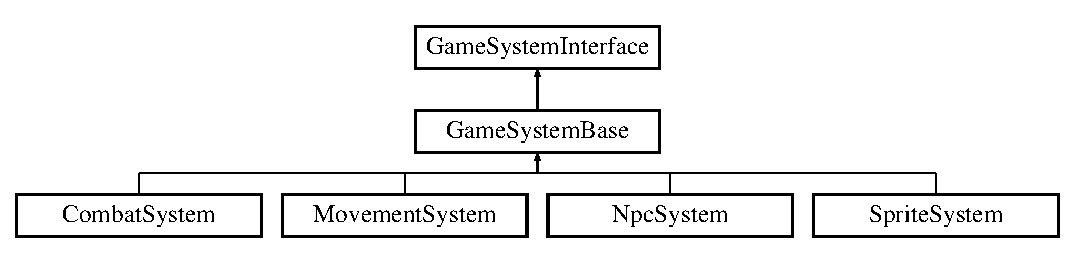
\includegraphics[height=2.957747cm]{classGameSystemInterface}
\end{center}
\end{figure}
\subsection*{Public Member Functions}
\begin{DoxyCompactItemize}
\item 
virtual void \hyperlink{classGameSystemInterface_a29079ef1f35027150b751c3fcb025091}{initialise} (\hyperlink{classGameEngineInterface}{Game\-Engine\-Interface} $\ast$engine)=0
\item 
virtual void \hyperlink{classGameSystemInterface_a386bcebd68725d6229f2fc84f1c762c7}{handle\-Event} (const \hyperlink{classEvent}{Event} $\ast$event)=0
\item 
virtual void \hyperlink{classGameSystemInterface_a531f5e7c6ca9881a67932cc4fded0a2e}{update} ()=0
\item 
virtual \hyperlink{classGameSystemInterface_ad4d59070ee87e375529ad1250850d1c6}{$\sim$\-Game\-System\-Interface} ()
\end{DoxyCompactItemize}


\subsection{Constructor \& Destructor Documentation}
\hypertarget{classGameSystemInterface_ad4d59070ee87e375529ad1250850d1c6}{\index{Game\-System\-Interface@{Game\-System\-Interface}!$\sim$\-Game\-System\-Interface@{$\sim$\-Game\-System\-Interface}}
\index{$\sim$\-Game\-System\-Interface@{$\sim$\-Game\-System\-Interface}!GameSystemInterface@{Game\-System\-Interface}}
\subsubsection[{$\sim$\-Game\-System\-Interface}]{\setlength{\rightskip}{0pt plus 5cm}virtual Game\-System\-Interface\-::$\sim$\-Game\-System\-Interface (
\begin{DoxyParamCaption}
{}
\end{DoxyParamCaption}
)\hspace{0.3cm}{\ttfamily [inline]}, {\ttfamily [virtual]}}}\label{classGameSystemInterface_ad4d59070ee87e375529ad1250850d1c6}


\subsection{Member Function Documentation}
\hypertarget{classGameSystemInterface_a386bcebd68725d6229f2fc84f1c762c7}{\index{Game\-System\-Interface@{Game\-System\-Interface}!handle\-Event@{handle\-Event}}
\index{handle\-Event@{handle\-Event}!GameSystemInterface@{Game\-System\-Interface}}
\subsubsection[{handle\-Event}]{\setlength{\rightskip}{0pt plus 5cm}virtual void Game\-System\-Interface\-::handle\-Event (
\begin{DoxyParamCaption}
\item[{const {\bf Event} $\ast$}]{event}
\end{DoxyParamCaption}
)\hspace{0.3cm}{\ttfamily [pure virtual]}}}\label{classGameSystemInterface_a386bcebd68725d6229f2fc84f1c762c7}


Implemented in \hyperlink{classGameSystemBase_a007b3ece290b1ad0dc3e397c5264d44d}{Game\-System\-Base}, \hyperlink{classSpriteSystem_a52c4236903911045c117fd4771300faf}{Sprite\-System}, \hyperlink{classMovementSystem_ac2c594a6deb6349a376cd72f189971a3}{Movement\-System}, \hyperlink{classNpcSystem_ad4c89f0e50944fc2f9dd7206411ced53}{Npc\-System}, and \hyperlink{classCombatSystem_afba5db4bb69a947c3a2303005f74d5d7}{Combat\-System}.

\hypertarget{classGameSystemInterface_a29079ef1f35027150b751c3fcb025091}{\index{Game\-System\-Interface@{Game\-System\-Interface}!initialise@{initialise}}
\index{initialise@{initialise}!GameSystemInterface@{Game\-System\-Interface}}
\subsubsection[{initialise}]{\setlength{\rightskip}{0pt plus 5cm}virtual void Game\-System\-Interface\-::initialise (
\begin{DoxyParamCaption}
\item[{{\bf Game\-Engine\-Interface} $\ast$}]{engine}
\end{DoxyParamCaption}
)\hspace{0.3cm}{\ttfamily [pure virtual]}}}\label{classGameSystemInterface_a29079ef1f35027150b751c3fcb025091}


Implemented in \hyperlink{classGameSystemBase_a55b4fc27cbfccd3c724c2e5984d78625}{Game\-System\-Base}.

\hypertarget{classGameSystemInterface_a531f5e7c6ca9881a67932cc4fded0a2e}{\index{Game\-System\-Interface@{Game\-System\-Interface}!update@{update}}
\index{update@{update}!GameSystemInterface@{Game\-System\-Interface}}
\subsubsection[{update}]{\setlength{\rightskip}{0pt plus 5cm}virtual void Game\-System\-Interface\-::update (
\begin{DoxyParamCaption}
{}
\end{DoxyParamCaption}
)\hspace{0.3cm}{\ttfamily [pure virtual]}}}\label{classGameSystemInterface_a531f5e7c6ca9881a67932cc4fded0a2e}


Implemented in \hyperlink{classGameSystemBase_a039d3086ac7fe50abdb110b569520d69}{Game\-System\-Base}, and \hyperlink{classNpcSystem_a88d87a8ec981e5cf1f4ed4340123a9d8}{Npc\-System}.



The documentation for this class was generated from the following file\-:\begin{DoxyCompactItemize}
\item 
\hyperlink{game__system__interface_8h}{game\-\_\-system\-\_\-interface.\-h}\end{DoxyCompactItemize}

\hypertarget{classGenerator}{\section{Generator Class Reference}
\label{classGenerator}\index{Generator@{Generator}}
}


{\ttfamily \#include $<$generator.\-h$>$}

Inheritance diagram for Generator\-:\begin{figure}[H]
\begin{center}
\leavevmode
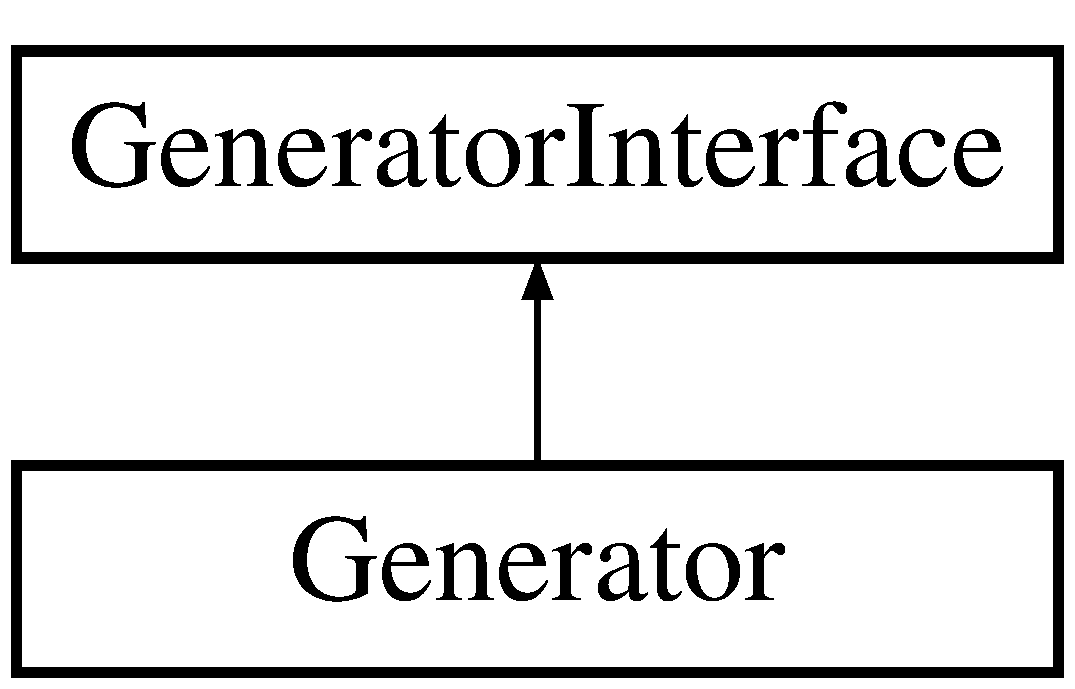
\includegraphics[height=2.000000cm]{classGenerator}
\end{center}
\end{figure}
\subsection*{Public Member Functions}
\begin{DoxyCompactItemize}
\item 
void \hyperlink{classGenerator_a3f690e7b3bb96571346bb51ca2adbe11}{initialise} (\hyperlink{classGameEngineInterface}{Game\-Engine\-Interface} $\ast$a\-\_\-engine)
\item 
void \hyperlink{classGenerator_a16cdfb04efdcc06650b99b2121d1b9b9}{generate} ()
\item 
unsigned int \& \hyperlink{classGenerator_adddb6dfba9dbda6ea3fd9d08ff250bde}{map\-Height} ()
\item 
unsigned int \& \hyperlink{classGenerator_a6558f2a519d5b8e67ecc3a6620a7fb5f}{map\-Width} ()
\item 
unsigned int \& \hyperlink{classGenerator_a9c3012dc9e8788ffd1014a6511238be2}{number\-Of\-Rooms} ()
\end{DoxyCompactItemize}
\subsection*{Private Member Functions}
\begin{DoxyCompactItemize}
\item 
bool \hyperlink{classGenerator_a5f40352b20fe2c4534523e18121cb0e6}{generate\-Room} (char $\ast$map)
\item 
void \hyperlink{classGenerator_a9daa14b13068fbe9efb1d14f55f629d1}{load\-Map} (char $\ast$map)
\end{DoxyCompactItemize}
\subsection*{Private Attributes}
\begin{DoxyCompactItemize}
\item 
\hyperlink{classGameEngineInterface}{Game\-Engine\-Interface} $\ast$ \hyperlink{classGenerator_a67bf71e434d74b280377b4f7acc3dc1d}{m\-\_\-engine}
\item 
unsigned int \hyperlink{classGenerator_a39fb4ca747e84f5422d313b4c57feb58}{m\-\_\-map\-Height}
\item 
unsigned int \hyperlink{classGenerator_aab82506c17f83cef3b1449ee32760e4b}{m\-\_\-map\-Width}
\item 
unsigned int \hyperlink{classGenerator_ad1cdb1fdc53ea37a7652c505dfdda628}{m\-\_\-rooms}
\end{DoxyCompactItemize}


\subsection{Member Function Documentation}
\hypertarget{classGenerator_a16cdfb04efdcc06650b99b2121d1b9b9}{\index{Generator@{Generator}!generate@{generate}}
\index{generate@{generate}!Generator@{Generator}}
\subsubsection[{generate}]{\setlength{\rightskip}{0pt plus 5cm}void Generator\-::generate (
\begin{DoxyParamCaption}
{}
\end{DoxyParamCaption}
)\hspace{0.3cm}{\ttfamily [virtual]}}}\label{classGenerator_a16cdfb04efdcc06650b99b2121d1b9b9}


Implements \hyperlink{classGeneratorInterface_a428214973b697b3e52a9993a730c6678}{Generator\-Interface}.

\hypertarget{classGenerator_a5f40352b20fe2c4534523e18121cb0e6}{\index{Generator@{Generator}!generate\-Room@{generate\-Room}}
\index{generate\-Room@{generate\-Room}!Generator@{Generator}}
\subsubsection[{generate\-Room}]{\setlength{\rightskip}{0pt plus 5cm}bool Generator\-::generate\-Room (
\begin{DoxyParamCaption}
\item[{char $\ast$}]{map}
\end{DoxyParamCaption}
)\hspace{0.3cm}{\ttfamily [private]}}}\label{classGenerator_a5f40352b20fe2c4534523e18121cb0e6}
\hypertarget{classGenerator_a3f690e7b3bb96571346bb51ca2adbe11}{\index{Generator@{Generator}!initialise@{initialise}}
\index{initialise@{initialise}!Generator@{Generator}}
\subsubsection[{initialise}]{\setlength{\rightskip}{0pt plus 5cm}void Generator\-::initialise (
\begin{DoxyParamCaption}
\item[{{\bf Game\-Engine\-Interface} $\ast$}]{a\-\_\-engine}
\end{DoxyParamCaption}
)\hspace{0.3cm}{\ttfamily [inline]}, {\ttfamily [virtual]}}}\label{classGenerator_a3f690e7b3bb96571346bb51ca2adbe11}


Implements \hyperlink{classGeneratorInterface_ae0466ff42c3ea7f068df9e70f3f12171}{Generator\-Interface}.

\hypertarget{classGenerator_a9daa14b13068fbe9efb1d14f55f629d1}{\index{Generator@{Generator}!load\-Map@{load\-Map}}
\index{load\-Map@{load\-Map}!Generator@{Generator}}
\subsubsection[{load\-Map}]{\setlength{\rightskip}{0pt plus 5cm}void Generator\-::load\-Map (
\begin{DoxyParamCaption}
\item[{char $\ast$}]{map}
\end{DoxyParamCaption}
)\hspace{0.3cm}{\ttfamily [private]}}}\label{classGenerator_a9daa14b13068fbe9efb1d14f55f629d1}
\hypertarget{classGenerator_adddb6dfba9dbda6ea3fd9d08ff250bde}{\index{Generator@{Generator}!map\-Height@{map\-Height}}
\index{map\-Height@{map\-Height}!Generator@{Generator}}
\subsubsection[{map\-Height}]{\setlength{\rightskip}{0pt plus 5cm}unsigned int\& Generator\-::map\-Height (
\begin{DoxyParamCaption}
{}
\end{DoxyParamCaption}
)\hspace{0.3cm}{\ttfamily [inline]}, {\ttfamily [virtual]}}}\label{classGenerator_adddb6dfba9dbda6ea3fd9d08ff250bde}


Implements \hyperlink{classGeneratorInterface_adea269531309861c989f24e88caf2bc0}{Generator\-Interface}.

\hypertarget{classGenerator_a6558f2a519d5b8e67ecc3a6620a7fb5f}{\index{Generator@{Generator}!map\-Width@{map\-Width}}
\index{map\-Width@{map\-Width}!Generator@{Generator}}
\subsubsection[{map\-Width}]{\setlength{\rightskip}{0pt plus 5cm}unsigned int\& Generator\-::map\-Width (
\begin{DoxyParamCaption}
{}
\end{DoxyParamCaption}
)\hspace{0.3cm}{\ttfamily [inline]}, {\ttfamily [virtual]}}}\label{classGenerator_a6558f2a519d5b8e67ecc3a6620a7fb5f}


Implements \hyperlink{classGeneratorInterface_ac5748c03cd757f3025c002237d08bc2d}{Generator\-Interface}.

\hypertarget{classGenerator_a9c3012dc9e8788ffd1014a6511238be2}{\index{Generator@{Generator}!number\-Of\-Rooms@{number\-Of\-Rooms}}
\index{number\-Of\-Rooms@{number\-Of\-Rooms}!Generator@{Generator}}
\subsubsection[{number\-Of\-Rooms}]{\setlength{\rightskip}{0pt plus 5cm}unsigned int\& Generator\-::number\-Of\-Rooms (
\begin{DoxyParamCaption}
{}
\end{DoxyParamCaption}
)\hspace{0.3cm}{\ttfamily [inline]}, {\ttfamily [virtual]}}}\label{classGenerator_a9c3012dc9e8788ffd1014a6511238be2}


Implements \hyperlink{classGeneratorInterface_a23c74580b39bdec747a93a8ead071d9b}{Generator\-Interface}.



\subsection{Member Data Documentation}
\hypertarget{classGenerator_a67bf71e434d74b280377b4f7acc3dc1d}{\index{Generator@{Generator}!m\-\_\-engine@{m\-\_\-engine}}
\index{m\-\_\-engine@{m\-\_\-engine}!Generator@{Generator}}
\subsubsection[{m\-\_\-engine}]{\setlength{\rightskip}{0pt plus 5cm}{\bf Game\-Engine\-Interface}$\ast$ Generator\-::m\-\_\-engine\hspace{0.3cm}{\ttfamily [private]}}}\label{classGenerator_a67bf71e434d74b280377b4f7acc3dc1d}
\hypertarget{classGenerator_a39fb4ca747e84f5422d313b4c57feb58}{\index{Generator@{Generator}!m\-\_\-map\-Height@{m\-\_\-map\-Height}}
\index{m\-\_\-map\-Height@{m\-\_\-map\-Height}!Generator@{Generator}}
\subsubsection[{m\-\_\-map\-Height}]{\setlength{\rightskip}{0pt plus 5cm}unsigned int Generator\-::m\-\_\-map\-Height\hspace{0.3cm}{\ttfamily [private]}}}\label{classGenerator_a39fb4ca747e84f5422d313b4c57feb58}
\hypertarget{classGenerator_aab82506c17f83cef3b1449ee32760e4b}{\index{Generator@{Generator}!m\-\_\-map\-Width@{m\-\_\-map\-Width}}
\index{m\-\_\-map\-Width@{m\-\_\-map\-Width}!Generator@{Generator}}
\subsubsection[{m\-\_\-map\-Width}]{\setlength{\rightskip}{0pt plus 5cm}unsigned int Generator\-::m\-\_\-map\-Width\hspace{0.3cm}{\ttfamily [private]}}}\label{classGenerator_aab82506c17f83cef3b1449ee32760e4b}
\hypertarget{classGenerator_ad1cdb1fdc53ea37a7652c505dfdda628}{\index{Generator@{Generator}!m\-\_\-rooms@{m\-\_\-rooms}}
\index{m\-\_\-rooms@{m\-\_\-rooms}!Generator@{Generator}}
\subsubsection[{m\-\_\-rooms}]{\setlength{\rightskip}{0pt plus 5cm}unsigned int Generator\-::m\-\_\-rooms\hspace{0.3cm}{\ttfamily [private]}}}\label{classGenerator_ad1cdb1fdc53ea37a7652c505dfdda628}


The documentation for this class was generated from the following files\-:\begin{DoxyCompactItemize}
\item 
\hyperlink{generator_8h}{generator.\-h}\item 
\hyperlink{generator_8cpp}{generator.\-cpp}\end{DoxyCompactItemize}

\hypertarget{classGeneratorInterface}{\section{Generator\-Interface Class Reference}
\label{classGeneratorInterface}\index{Generator\-Interface@{Generator\-Interface}}
}


{\ttfamily \#include $<$generator\-\_\-interface.\-h$>$}

Inheritance diagram for Generator\-Interface\-:\begin{figure}[H]
\begin{center}
\leavevmode
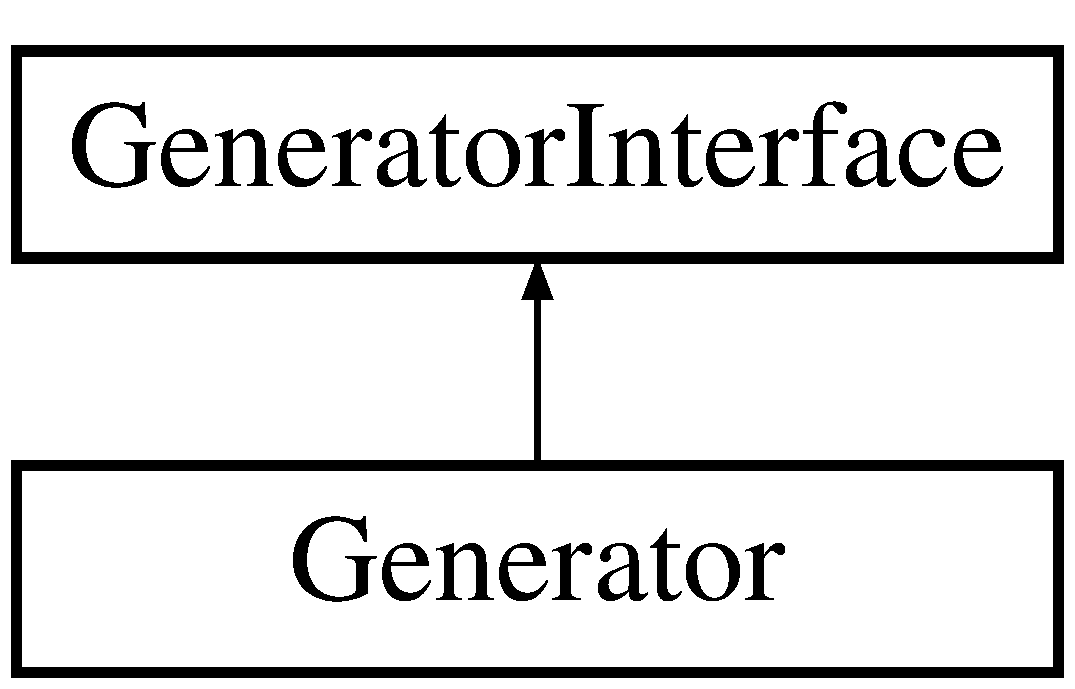
\includegraphics[height=2.000000cm]{classGeneratorInterface}
\end{center}
\end{figure}
\subsection*{Public Member Functions}
\begin{DoxyCompactItemize}
\item 
virtual \hyperlink{classGeneratorInterface_aa6474a64977a0b8a1613847672253f66}{$\sim$\-Generator\-Interface} ()
\item 
virtual void \hyperlink{classGeneratorInterface_ae0466ff42c3ea7f068df9e70f3f12171}{initialise} (\hyperlink{classGameEngineInterface}{Game\-Engine\-Interface} $\ast$)=0
\item 
virtual void \hyperlink{classGeneratorInterface_a428214973b697b3e52a9993a730c6678}{generate} ()=0
\item 
virtual unsigned int \& \hyperlink{classGeneratorInterface_adea269531309861c989f24e88caf2bc0}{map\-Height} ()=0
\item 
virtual unsigned int \& \hyperlink{classGeneratorInterface_ac5748c03cd757f3025c002237d08bc2d}{map\-Width} ()=0
\item 
virtual unsigned int \& \hyperlink{classGeneratorInterface_a23c74580b39bdec747a93a8ead071d9b}{number\-Of\-Rooms} ()=0
\end{DoxyCompactItemize}


\subsection{Constructor \& Destructor Documentation}
\hypertarget{classGeneratorInterface_aa6474a64977a0b8a1613847672253f66}{\index{Generator\-Interface@{Generator\-Interface}!$\sim$\-Generator\-Interface@{$\sim$\-Generator\-Interface}}
\index{$\sim$\-Generator\-Interface@{$\sim$\-Generator\-Interface}!GeneratorInterface@{Generator\-Interface}}
\subsubsection[{$\sim$\-Generator\-Interface}]{\setlength{\rightskip}{0pt plus 5cm}virtual Generator\-Interface\-::$\sim$\-Generator\-Interface (
\begin{DoxyParamCaption}
{}
\end{DoxyParamCaption}
)\hspace{0.3cm}{\ttfamily [inline]}, {\ttfamily [virtual]}}}\label{classGeneratorInterface_aa6474a64977a0b8a1613847672253f66}


\subsection{Member Function Documentation}
\hypertarget{classGeneratorInterface_a428214973b697b3e52a9993a730c6678}{\index{Generator\-Interface@{Generator\-Interface}!generate@{generate}}
\index{generate@{generate}!GeneratorInterface@{Generator\-Interface}}
\subsubsection[{generate}]{\setlength{\rightskip}{0pt plus 5cm}virtual void Generator\-Interface\-::generate (
\begin{DoxyParamCaption}
{}
\end{DoxyParamCaption}
)\hspace{0.3cm}{\ttfamily [pure virtual]}}}\label{classGeneratorInterface_a428214973b697b3e52a9993a730c6678}


Implemented in \hyperlink{classGenerator_a16cdfb04efdcc06650b99b2121d1b9b9}{Generator}.

\hypertarget{classGeneratorInterface_ae0466ff42c3ea7f068df9e70f3f12171}{\index{Generator\-Interface@{Generator\-Interface}!initialise@{initialise}}
\index{initialise@{initialise}!GeneratorInterface@{Generator\-Interface}}
\subsubsection[{initialise}]{\setlength{\rightskip}{0pt plus 5cm}virtual void Generator\-Interface\-::initialise (
\begin{DoxyParamCaption}
\item[{{\bf Game\-Engine\-Interface} $\ast$}]{}
\end{DoxyParamCaption}
)\hspace{0.3cm}{\ttfamily [pure virtual]}}}\label{classGeneratorInterface_ae0466ff42c3ea7f068df9e70f3f12171}


Implemented in \hyperlink{classGenerator_a3f690e7b3bb96571346bb51ca2adbe11}{Generator}.

\hypertarget{classGeneratorInterface_adea269531309861c989f24e88caf2bc0}{\index{Generator\-Interface@{Generator\-Interface}!map\-Height@{map\-Height}}
\index{map\-Height@{map\-Height}!GeneratorInterface@{Generator\-Interface}}
\subsubsection[{map\-Height}]{\setlength{\rightskip}{0pt plus 5cm}virtual unsigned int\& Generator\-Interface\-::map\-Height (
\begin{DoxyParamCaption}
{}
\end{DoxyParamCaption}
)\hspace{0.3cm}{\ttfamily [pure virtual]}}}\label{classGeneratorInterface_adea269531309861c989f24e88caf2bc0}


Implemented in \hyperlink{classGenerator_adddb6dfba9dbda6ea3fd9d08ff250bde}{Generator}.

\hypertarget{classGeneratorInterface_ac5748c03cd757f3025c002237d08bc2d}{\index{Generator\-Interface@{Generator\-Interface}!map\-Width@{map\-Width}}
\index{map\-Width@{map\-Width}!GeneratorInterface@{Generator\-Interface}}
\subsubsection[{map\-Width}]{\setlength{\rightskip}{0pt plus 5cm}virtual unsigned int\& Generator\-Interface\-::map\-Width (
\begin{DoxyParamCaption}
{}
\end{DoxyParamCaption}
)\hspace{0.3cm}{\ttfamily [pure virtual]}}}\label{classGeneratorInterface_ac5748c03cd757f3025c002237d08bc2d}


Implemented in \hyperlink{classGenerator_a6558f2a519d5b8e67ecc3a6620a7fb5f}{Generator}.

\hypertarget{classGeneratorInterface_a23c74580b39bdec747a93a8ead071d9b}{\index{Generator\-Interface@{Generator\-Interface}!number\-Of\-Rooms@{number\-Of\-Rooms}}
\index{number\-Of\-Rooms@{number\-Of\-Rooms}!GeneratorInterface@{Generator\-Interface}}
\subsubsection[{number\-Of\-Rooms}]{\setlength{\rightskip}{0pt plus 5cm}virtual unsigned int\& Generator\-Interface\-::number\-Of\-Rooms (
\begin{DoxyParamCaption}
{}
\end{DoxyParamCaption}
)\hspace{0.3cm}{\ttfamily [pure virtual]}}}\label{classGeneratorInterface_a23c74580b39bdec747a93a8ead071d9b}


Implemented in \hyperlink{classGenerator_a9c3012dc9e8788ffd1014a6511238be2}{Generator}.



The documentation for this class was generated from the following file\-:\begin{DoxyCompactItemize}
\item 
\hyperlink{generator__interface_8h}{generator\-\_\-interface.\-h}\end{DoxyCompactItemize}

\hypertarget{classGraphics}{\section{Graphics Class Reference}
\label{classGraphics}\index{Graphics@{Graphics}}
}


{\ttfamily \#include $<$graphics.\-h$>$}

Inheritance diagram for Graphics\-:\begin{figure}[H]
\begin{center}
\leavevmode
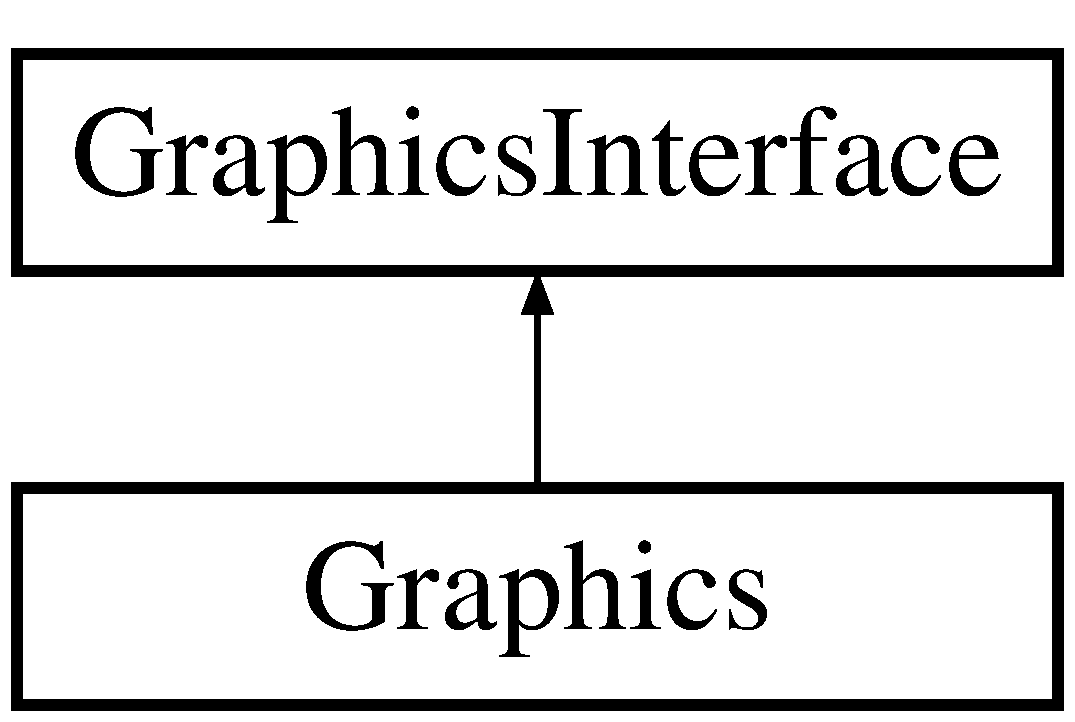
\includegraphics[height=2.000000cm]{classGraphics}
\end{center}
\end{figure}
\subsection*{Public Member Functions}
\begin{DoxyCompactItemize}
\item 
virtual void \hyperlink{classGraphics_a66b2e289d2963868a7c79cee2941942b}{initialise} (int argc, char $\ast$$\ast$argv)
\item 
virtual void \hyperlink{classGraphics_aec5a37f9c17f75ced39db3cf1167fa4a}{spin} ()
\item 
virtual void \hyperlink{classGraphics_adcad998ac1340c761645ed0c00412522}{draw\-String} (int y, int x, const char $\ast$s)
\item 
virtual void \hyperlink{classGraphics_a2bf550e92188fd991939f5d1429b7d4d}{draw\-Tile} (int y, int x, unsigned int tile, \hyperlink{classColor}{Color} fg, \hyperlink{classColor}{Color} bg)
\item 
virtual void \hyperlink{classGraphics_a0193f21f1333dcbe93c4759fcf1fb7d7}{draw\-Border} (int y, int x, int height, int width)
\item 
virtual void \hyperlink{classGraphics_a3bb97ab19f7abb7ad61f17614bdeb82e}{begin\-Screen\-Update} ()
\item 
virtual void \hyperlink{classGraphics_aaf60fa961c17a3007f3bb8ebddaa3006}{end\-Screen\-Update} ()
\item 
virtual void \hyperlink{classGraphics_a92c097e9ac471b361c9e72af40898cb9}{set\-Keyboard\-Func} (\hyperlink{graphics__interface_8h_ae8b5bc37678d3ba69d310ca3c6e7393f}{Keyboard\-Func\-Ptr} func)
\item 
virtual void \hyperlink{classGraphics_aaf99a21378b7bbc86d665212d8151f77}{set\-Keyboard\-Up\-Func} (\hyperlink{graphics__interface_8h_ae8b5bc37678d3ba69d310ca3c6e7393f}{Keyboard\-Func\-Ptr} func)
\item 
virtual void \hyperlink{classGraphics_a134f47e4496f56affd656660c6037e1d}{set\-Display\-Func} (\hyperlink{graphics__interface_8h_a71f99ab7c9bb1fb2ae09a63a9d4d422b}{Display\-Func\-Ptr} func)
\item 
virtual void \hyperlink{classGraphics_aa20c019aad3ded8495620a1b6d9bbbc1}{set\-Mouse\-Func} (\hyperlink{graphics__interface_8h_a60715b4a82a8c09c76ddd8b483d768ef}{Mouse\-Func\-Ptr} func)
\end{DoxyCompactItemize}
\subsection*{Private Attributes}
\begin{DoxyCompactItemize}
\item 
\hyperlink{classConfigManager}{Config\-Manager} \hyperlink{classGraphics_ab564a5716ae0bdaa73dde9f257e769d6}{m\-\_\-config}
\end{DoxyCompactItemize}


\subsection{Member Function Documentation}
\hypertarget{classGraphics_a3bb97ab19f7abb7ad61f17614bdeb82e}{\index{Graphics@{Graphics}!begin\-Screen\-Update@{begin\-Screen\-Update}}
\index{begin\-Screen\-Update@{begin\-Screen\-Update}!Graphics@{Graphics}}
\subsubsection[{begin\-Screen\-Update}]{\setlength{\rightskip}{0pt plus 5cm}void Graphics\-::begin\-Screen\-Update (
\begin{DoxyParamCaption}
{}
\end{DoxyParamCaption}
)\hspace{0.3cm}{\ttfamily [virtual]}}}\label{classGraphics_a3bb97ab19f7abb7ad61f17614bdeb82e}


Implements \hyperlink{classGraphicsInterface_a31ab6e9004825ec7ea337c2dd530114a}{Graphics\-Interface}.

\hypertarget{classGraphics_a0193f21f1333dcbe93c4759fcf1fb7d7}{\index{Graphics@{Graphics}!draw\-Border@{draw\-Border}}
\index{draw\-Border@{draw\-Border}!Graphics@{Graphics}}
\subsubsection[{draw\-Border}]{\setlength{\rightskip}{0pt plus 5cm}void Graphics\-::draw\-Border (
\begin{DoxyParamCaption}
\item[{int}]{y, }
\item[{int}]{x, }
\item[{int}]{height, }
\item[{int}]{width}
\end{DoxyParamCaption}
)\hspace{0.3cm}{\ttfamily [virtual]}}}\label{classGraphics_a0193f21f1333dcbe93c4759fcf1fb7d7}


Implements \hyperlink{classGraphicsInterface_a5ee4a7b699755b8348955b7e166c154b}{Graphics\-Interface}.

\hypertarget{classGraphics_adcad998ac1340c761645ed0c00412522}{\index{Graphics@{Graphics}!draw\-String@{draw\-String}}
\index{draw\-String@{draw\-String}!Graphics@{Graphics}}
\subsubsection[{draw\-String}]{\setlength{\rightskip}{0pt plus 5cm}void Graphics\-::draw\-String (
\begin{DoxyParamCaption}
\item[{int}]{y, }
\item[{int}]{x, }
\item[{const char $\ast$}]{s}
\end{DoxyParamCaption}
)\hspace{0.3cm}{\ttfamily [virtual]}}}\label{classGraphics_adcad998ac1340c761645ed0c00412522}


Implements \hyperlink{classGraphicsInterface_aa58e5f8df996b8d64a456dedaa3bb549}{Graphics\-Interface}.

\hypertarget{classGraphics_a2bf550e92188fd991939f5d1429b7d4d}{\index{Graphics@{Graphics}!draw\-Tile@{draw\-Tile}}
\index{draw\-Tile@{draw\-Tile}!Graphics@{Graphics}}
\subsubsection[{draw\-Tile}]{\setlength{\rightskip}{0pt plus 5cm}void Graphics\-::draw\-Tile (
\begin{DoxyParamCaption}
\item[{int}]{y, }
\item[{int}]{x, }
\item[{unsigned int}]{tile, }
\item[{{\bf Color}}]{fg, }
\item[{{\bf Color}}]{bg}
\end{DoxyParamCaption}
)\hspace{0.3cm}{\ttfamily [virtual]}}}\label{classGraphics_a2bf550e92188fd991939f5d1429b7d4d}


Implements \hyperlink{classGraphicsInterface_af46b9a83803b47cda354449d3afced25}{Graphics\-Interface}.

\hypertarget{classGraphics_aaf60fa961c17a3007f3bb8ebddaa3006}{\index{Graphics@{Graphics}!end\-Screen\-Update@{end\-Screen\-Update}}
\index{end\-Screen\-Update@{end\-Screen\-Update}!Graphics@{Graphics}}
\subsubsection[{end\-Screen\-Update}]{\setlength{\rightskip}{0pt plus 5cm}void Graphics\-::end\-Screen\-Update (
\begin{DoxyParamCaption}
{}
\end{DoxyParamCaption}
)\hspace{0.3cm}{\ttfamily [virtual]}}}\label{classGraphics_aaf60fa961c17a3007f3bb8ebddaa3006}


Implements \hyperlink{classGraphicsInterface_aa6d993639a30dee68aa9aacd9ba1ad5c}{Graphics\-Interface}.

\hypertarget{classGraphics_a66b2e289d2963868a7c79cee2941942b}{\index{Graphics@{Graphics}!initialise@{initialise}}
\index{initialise@{initialise}!Graphics@{Graphics}}
\subsubsection[{initialise}]{\setlength{\rightskip}{0pt plus 5cm}void Graphics\-::initialise (
\begin{DoxyParamCaption}
\item[{int}]{argc, }
\item[{char $\ast$$\ast$}]{argv}
\end{DoxyParamCaption}
)\hspace{0.3cm}{\ttfamily [virtual]}}}\label{classGraphics_a66b2e289d2963868a7c79cee2941942b}


Implements \hyperlink{classGraphicsInterface_a3a47a8e69b8f31a962bed451b3f7c498}{Graphics\-Interface}.

\hypertarget{classGraphics_a134f47e4496f56affd656660c6037e1d}{\index{Graphics@{Graphics}!set\-Display\-Func@{set\-Display\-Func}}
\index{set\-Display\-Func@{set\-Display\-Func}!Graphics@{Graphics}}
\subsubsection[{set\-Display\-Func}]{\setlength{\rightskip}{0pt plus 5cm}void Graphics\-::set\-Display\-Func (
\begin{DoxyParamCaption}
\item[{{\bf Display\-Func\-Ptr}}]{func}
\end{DoxyParamCaption}
)\hspace{0.3cm}{\ttfamily [virtual]}}}\label{classGraphics_a134f47e4496f56affd656660c6037e1d}


Implements \hyperlink{classGraphicsInterface_a83af0372a01cd878a724ed81722b62cd}{Graphics\-Interface}.

\hypertarget{classGraphics_a92c097e9ac471b361c9e72af40898cb9}{\index{Graphics@{Graphics}!set\-Keyboard\-Func@{set\-Keyboard\-Func}}
\index{set\-Keyboard\-Func@{set\-Keyboard\-Func}!Graphics@{Graphics}}
\subsubsection[{set\-Keyboard\-Func}]{\setlength{\rightskip}{0pt plus 5cm}void Graphics\-::set\-Keyboard\-Func (
\begin{DoxyParamCaption}
\item[{{\bf Keyboard\-Func\-Ptr}}]{func}
\end{DoxyParamCaption}
)\hspace{0.3cm}{\ttfamily [virtual]}}}\label{classGraphics_a92c097e9ac471b361c9e72af40898cb9}


Implements \hyperlink{classGraphicsInterface_a306cf250c51013ff35c3a657d694f921}{Graphics\-Interface}.

\hypertarget{classGraphics_aaf99a21378b7bbc86d665212d8151f77}{\index{Graphics@{Graphics}!set\-Keyboard\-Up\-Func@{set\-Keyboard\-Up\-Func}}
\index{set\-Keyboard\-Up\-Func@{set\-Keyboard\-Up\-Func}!Graphics@{Graphics}}
\subsubsection[{set\-Keyboard\-Up\-Func}]{\setlength{\rightskip}{0pt plus 5cm}void Graphics\-::set\-Keyboard\-Up\-Func (
\begin{DoxyParamCaption}
\item[{{\bf Keyboard\-Func\-Ptr}}]{func}
\end{DoxyParamCaption}
)\hspace{0.3cm}{\ttfamily [virtual]}}}\label{classGraphics_aaf99a21378b7bbc86d665212d8151f77}


Implements \hyperlink{classGraphicsInterface_ac79f6dfb01b2915fb2ce51efabd692c5}{Graphics\-Interface}.

\hypertarget{classGraphics_aa20c019aad3ded8495620a1b6d9bbbc1}{\index{Graphics@{Graphics}!set\-Mouse\-Func@{set\-Mouse\-Func}}
\index{set\-Mouse\-Func@{set\-Mouse\-Func}!Graphics@{Graphics}}
\subsubsection[{set\-Mouse\-Func}]{\setlength{\rightskip}{0pt plus 5cm}void Graphics\-::set\-Mouse\-Func (
\begin{DoxyParamCaption}
\item[{{\bf Mouse\-Func\-Ptr}}]{func}
\end{DoxyParamCaption}
)\hspace{0.3cm}{\ttfamily [virtual]}}}\label{classGraphics_aa20c019aad3ded8495620a1b6d9bbbc1}


Implements \hyperlink{classGraphicsInterface_a5730723c0b0e2d676ff11882076c1e6c}{Graphics\-Interface}.

\hypertarget{classGraphics_aec5a37f9c17f75ced39db3cf1167fa4a}{\index{Graphics@{Graphics}!spin@{spin}}
\index{spin@{spin}!Graphics@{Graphics}}
\subsubsection[{spin}]{\setlength{\rightskip}{0pt plus 5cm}void Graphics\-::spin (
\begin{DoxyParamCaption}
{}
\end{DoxyParamCaption}
)\hspace{0.3cm}{\ttfamily [virtual]}}}\label{classGraphics_aec5a37f9c17f75ced39db3cf1167fa4a}


Implements \hyperlink{classGraphicsInterface_a7eab61b47e23240090b339151809eb1d}{Graphics\-Interface}.



\subsection{Member Data Documentation}
\hypertarget{classGraphics_ab564a5716ae0bdaa73dde9f257e769d6}{\index{Graphics@{Graphics}!m\-\_\-config@{m\-\_\-config}}
\index{m\-\_\-config@{m\-\_\-config}!Graphics@{Graphics}}
\subsubsection[{m\-\_\-config}]{\setlength{\rightskip}{0pt plus 5cm}{\bf Config\-Manager} Graphics\-::m\-\_\-config\hspace{0.3cm}{\ttfamily [private]}}}\label{classGraphics_ab564a5716ae0bdaa73dde9f257e769d6}


The documentation for this class was generated from the following files\-:\begin{DoxyCompactItemize}
\item 
\hyperlink{graphics_8h}{graphics.\-h}\item 
\hyperlink{graphics_8cpp}{graphics.\-cpp}\end{DoxyCompactItemize}

\hypertarget{classGraphicsInterface}{\section{Graphics\-Interface Class Reference}
\label{classGraphicsInterface}\index{Graphics\-Interface@{Graphics\-Interface}}
}


{\ttfamily \#include $<$graphics\-\_\-interface.\-h$>$}

Inheritance diagram for Graphics\-Interface\-:\begin{figure}[H]
\begin{center}
\leavevmode
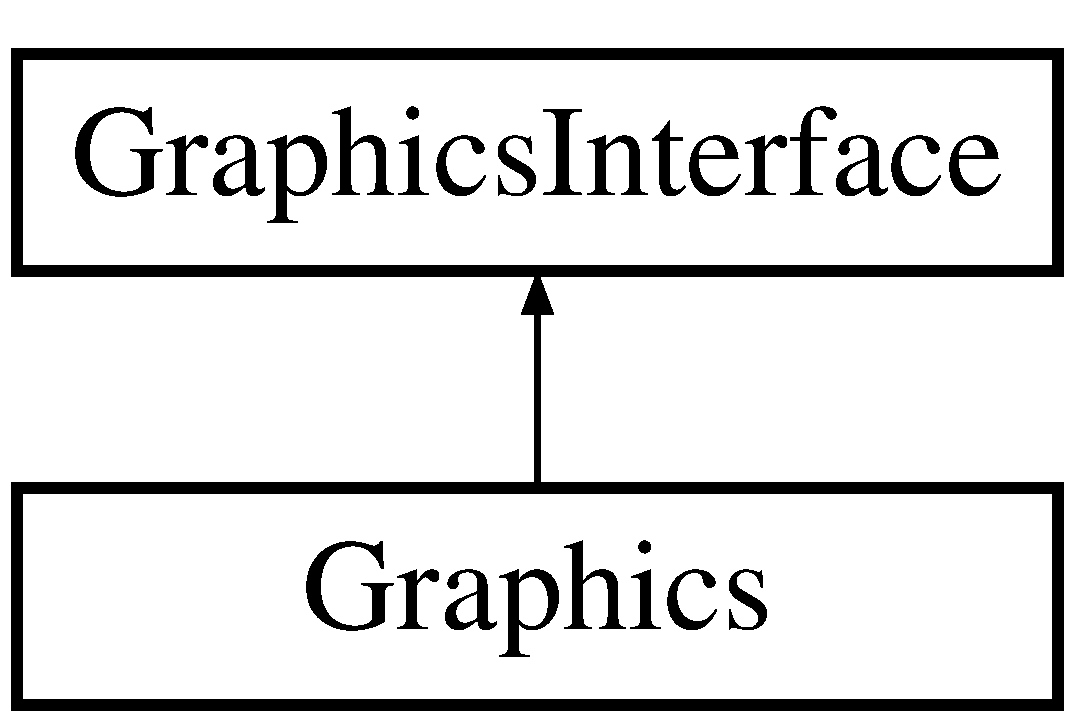
\includegraphics[height=2.000000cm]{classGraphicsInterface}
\end{center}
\end{figure}
\subsection*{Public Member Functions}
\begin{DoxyCompactItemize}
\item 
virtual \hyperlink{classGraphicsInterface_ada388bd981edb66e9d47c23a3ab11e70}{$\sim$\-Graphics\-Interface} ()
\item 
virtual void \hyperlink{classGraphicsInterface_a3a47a8e69b8f31a962bed451b3f7c498}{initialise} (int argc, char $\ast$$\ast$argv)=0
\item 
virtual void \hyperlink{classGraphicsInterface_a7eab61b47e23240090b339151809eb1d}{spin} ()=0
\item 
virtual void \hyperlink{classGraphicsInterface_a31ab6e9004825ec7ea337c2dd530114a}{begin\-Screen\-Update} ()=0
\item 
virtual void \hyperlink{classGraphicsInterface_aa6d993639a30dee68aa9aacd9ba1ad5c}{end\-Screen\-Update} ()=0
\item 
virtual void \hyperlink{classGraphicsInterface_aa58e5f8df996b8d64a456dedaa3bb549}{draw\-String} (int y, int x, const char $\ast$s)=0
\item 
virtual void \hyperlink{classGraphicsInterface_af46b9a83803b47cda354449d3afced25}{draw\-Tile} (int y, int x, unsigned int tile, \hyperlink{classColor}{Color} fg, \hyperlink{classColor}{Color} bg)=0
\item 
virtual void \hyperlink{classGraphicsInterface_a5ee4a7b699755b8348955b7e166c154b}{draw\-Border} (int y, int x, int height, int width)=0
\item 
virtual void \hyperlink{classGraphicsInterface_a306cf250c51013ff35c3a657d694f921}{set\-Keyboard\-Func} (\hyperlink{graphics__interface_8h_ae8b5bc37678d3ba69d310ca3c6e7393f}{Keyboard\-Func\-Ptr} func)=0
\item 
virtual void \hyperlink{classGraphicsInterface_ac79f6dfb01b2915fb2ce51efabd692c5}{set\-Keyboard\-Up\-Func} (\hyperlink{graphics__interface_8h_ae8b5bc37678d3ba69d310ca3c6e7393f}{Keyboard\-Func\-Ptr} func)=0
\item 
virtual void \hyperlink{classGraphicsInterface_a83af0372a01cd878a724ed81722b62cd}{set\-Display\-Func} (\hyperlink{graphics__interface_8h_a71f99ab7c9bb1fb2ae09a63a9d4d422b}{Display\-Func\-Ptr} func)=0
\item 
virtual void \hyperlink{classGraphicsInterface_a5730723c0b0e2d676ff11882076c1e6c}{set\-Mouse\-Func} (\hyperlink{graphics__interface_8h_a60715b4a82a8c09c76ddd8b483d768ef}{Mouse\-Func\-Ptr} func)=0
\end{DoxyCompactItemize}


\subsection{Constructor \& Destructor Documentation}
\hypertarget{classGraphicsInterface_ada388bd981edb66e9d47c23a3ab11e70}{\index{Graphics\-Interface@{Graphics\-Interface}!$\sim$\-Graphics\-Interface@{$\sim$\-Graphics\-Interface}}
\index{$\sim$\-Graphics\-Interface@{$\sim$\-Graphics\-Interface}!GraphicsInterface@{Graphics\-Interface}}
\subsubsection[{$\sim$\-Graphics\-Interface}]{\setlength{\rightskip}{0pt plus 5cm}virtual Graphics\-Interface\-::$\sim$\-Graphics\-Interface (
\begin{DoxyParamCaption}
{}
\end{DoxyParamCaption}
)\hspace{0.3cm}{\ttfamily [inline]}, {\ttfamily [virtual]}}}\label{classGraphicsInterface_ada388bd981edb66e9d47c23a3ab11e70}


\subsection{Member Function Documentation}
\hypertarget{classGraphicsInterface_a31ab6e9004825ec7ea337c2dd530114a}{\index{Graphics\-Interface@{Graphics\-Interface}!begin\-Screen\-Update@{begin\-Screen\-Update}}
\index{begin\-Screen\-Update@{begin\-Screen\-Update}!GraphicsInterface@{Graphics\-Interface}}
\subsubsection[{begin\-Screen\-Update}]{\setlength{\rightskip}{0pt plus 5cm}virtual void Graphics\-Interface\-::begin\-Screen\-Update (
\begin{DoxyParamCaption}
{}
\end{DoxyParamCaption}
)\hspace{0.3cm}{\ttfamily [pure virtual]}}}\label{classGraphicsInterface_a31ab6e9004825ec7ea337c2dd530114a}


Implemented in \hyperlink{classGraphics_a3bb97ab19f7abb7ad61f17614bdeb82e}{Graphics}.

\hypertarget{classGraphicsInterface_a5ee4a7b699755b8348955b7e166c154b}{\index{Graphics\-Interface@{Graphics\-Interface}!draw\-Border@{draw\-Border}}
\index{draw\-Border@{draw\-Border}!GraphicsInterface@{Graphics\-Interface}}
\subsubsection[{draw\-Border}]{\setlength{\rightskip}{0pt plus 5cm}virtual void Graphics\-Interface\-::draw\-Border (
\begin{DoxyParamCaption}
\item[{int}]{y, }
\item[{int}]{x, }
\item[{int}]{height, }
\item[{int}]{width}
\end{DoxyParamCaption}
)\hspace{0.3cm}{\ttfamily [pure virtual]}}}\label{classGraphicsInterface_a5ee4a7b699755b8348955b7e166c154b}


Implemented in \hyperlink{classGraphics_a0193f21f1333dcbe93c4759fcf1fb7d7}{Graphics}.

\hypertarget{classGraphicsInterface_aa58e5f8df996b8d64a456dedaa3bb549}{\index{Graphics\-Interface@{Graphics\-Interface}!draw\-String@{draw\-String}}
\index{draw\-String@{draw\-String}!GraphicsInterface@{Graphics\-Interface}}
\subsubsection[{draw\-String}]{\setlength{\rightskip}{0pt plus 5cm}virtual void Graphics\-Interface\-::draw\-String (
\begin{DoxyParamCaption}
\item[{int}]{y, }
\item[{int}]{x, }
\item[{const char $\ast$}]{s}
\end{DoxyParamCaption}
)\hspace{0.3cm}{\ttfamily [pure virtual]}}}\label{classGraphicsInterface_aa58e5f8df996b8d64a456dedaa3bb549}


Implemented in \hyperlink{classGraphics_adcad998ac1340c761645ed0c00412522}{Graphics}.

\hypertarget{classGraphicsInterface_af46b9a83803b47cda354449d3afced25}{\index{Graphics\-Interface@{Graphics\-Interface}!draw\-Tile@{draw\-Tile}}
\index{draw\-Tile@{draw\-Tile}!GraphicsInterface@{Graphics\-Interface}}
\subsubsection[{draw\-Tile}]{\setlength{\rightskip}{0pt plus 5cm}virtual void Graphics\-Interface\-::draw\-Tile (
\begin{DoxyParamCaption}
\item[{int}]{y, }
\item[{int}]{x, }
\item[{unsigned int}]{tile, }
\item[{{\bf Color}}]{fg, }
\item[{{\bf Color}}]{bg}
\end{DoxyParamCaption}
)\hspace{0.3cm}{\ttfamily [pure virtual]}}}\label{classGraphicsInterface_af46b9a83803b47cda354449d3afced25}


Implemented in \hyperlink{classGraphics_a2bf550e92188fd991939f5d1429b7d4d}{Graphics}.

\hypertarget{classGraphicsInterface_aa6d993639a30dee68aa9aacd9ba1ad5c}{\index{Graphics\-Interface@{Graphics\-Interface}!end\-Screen\-Update@{end\-Screen\-Update}}
\index{end\-Screen\-Update@{end\-Screen\-Update}!GraphicsInterface@{Graphics\-Interface}}
\subsubsection[{end\-Screen\-Update}]{\setlength{\rightskip}{0pt plus 5cm}virtual void Graphics\-Interface\-::end\-Screen\-Update (
\begin{DoxyParamCaption}
{}
\end{DoxyParamCaption}
)\hspace{0.3cm}{\ttfamily [pure virtual]}}}\label{classGraphicsInterface_aa6d993639a30dee68aa9aacd9ba1ad5c}


Implemented in \hyperlink{classGraphics_aaf60fa961c17a3007f3bb8ebddaa3006}{Graphics}.

\hypertarget{classGraphicsInterface_a3a47a8e69b8f31a962bed451b3f7c498}{\index{Graphics\-Interface@{Graphics\-Interface}!initialise@{initialise}}
\index{initialise@{initialise}!GraphicsInterface@{Graphics\-Interface}}
\subsubsection[{initialise}]{\setlength{\rightskip}{0pt plus 5cm}virtual void Graphics\-Interface\-::initialise (
\begin{DoxyParamCaption}
\item[{int}]{argc, }
\item[{char $\ast$$\ast$}]{argv}
\end{DoxyParamCaption}
)\hspace{0.3cm}{\ttfamily [pure virtual]}}}\label{classGraphicsInterface_a3a47a8e69b8f31a962bed451b3f7c498}


Implemented in \hyperlink{classGraphics_a66b2e289d2963868a7c79cee2941942b}{Graphics}.

\hypertarget{classGraphicsInterface_a83af0372a01cd878a724ed81722b62cd}{\index{Graphics\-Interface@{Graphics\-Interface}!set\-Display\-Func@{set\-Display\-Func}}
\index{set\-Display\-Func@{set\-Display\-Func}!GraphicsInterface@{Graphics\-Interface}}
\subsubsection[{set\-Display\-Func}]{\setlength{\rightskip}{0pt plus 5cm}virtual void Graphics\-Interface\-::set\-Display\-Func (
\begin{DoxyParamCaption}
\item[{{\bf Display\-Func\-Ptr}}]{func}
\end{DoxyParamCaption}
)\hspace{0.3cm}{\ttfamily [pure virtual]}}}\label{classGraphicsInterface_a83af0372a01cd878a724ed81722b62cd}


Implemented in \hyperlink{classGraphics_a134f47e4496f56affd656660c6037e1d}{Graphics}.

\hypertarget{classGraphicsInterface_a306cf250c51013ff35c3a657d694f921}{\index{Graphics\-Interface@{Graphics\-Interface}!set\-Keyboard\-Func@{set\-Keyboard\-Func}}
\index{set\-Keyboard\-Func@{set\-Keyboard\-Func}!GraphicsInterface@{Graphics\-Interface}}
\subsubsection[{set\-Keyboard\-Func}]{\setlength{\rightskip}{0pt plus 5cm}virtual void Graphics\-Interface\-::set\-Keyboard\-Func (
\begin{DoxyParamCaption}
\item[{{\bf Keyboard\-Func\-Ptr}}]{func}
\end{DoxyParamCaption}
)\hspace{0.3cm}{\ttfamily [pure virtual]}}}\label{classGraphicsInterface_a306cf250c51013ff35c3a657d694f921}


Implemented in \hyperlink{classGraphics_a92c097e9ac471b361c9e72af40898cb9}{Graphics}.

\hypertarget{classGraphicsInterface_ac79f6dfb01b2915fb2ce51efabd692c5}{\index{Graphics\-Interface@{Graphics\-Interface}!set\-Keyboard\-Up\-Func@{set\-Keyboard\-Up\-Func}}
\index{set\-Keyboard\-Up\-Func@{set\-Keyboard\-Up\-Func}!GraphicsInterface@{Graphics\-Interface}}
\subsubsection[{set\-Keyboard\-Up\-Func}]{\setlength{\rightskip}{0pt plus 5cm}virtual void Graphics\-Interface\-::set\-Keyboard\-Up\-Func (
\begin{DoxyParamCaption}
\item[{{\bf Keyboard\-Func\-Ptr}}]{func}
\end{DoxyParamCaption}
)\hspace{0.3cm}{\ttfamily [pure virtual]}}}\label{classGraphicsInterface_ac79f6dfb01b2915fb2ce51efabd692c5}


Implemented in \hyperlink{classGraphics_aaf99a21378b7bbc86d665212d8151f77}{Graphics}.

\hypertarget{classGraphicsInterface_a5730723c0b0e2d676ff11882076c1e6c}{\index{Graphics\-Interface@{Graphics\-Interface}!set\-Mouse\-Func@{set\-Mouse\-Func}}
\index{set\-Mouse\-Func@{set\-Mouse\-Func}!GraphicsInterface@{Graphics\-Interface}}
\subsubsection[{set\-Mouse\-Func}]{\setlength{\rightskip}{0pt plus 5cm}virtual void Graphics\-Interface\-::set\-Mouse\-Func (
\begin{DoxyParamCaption}
\item[{{\bf Mouse\-Func\-Ptr}}]{func}
\end{DoxyParamCaption}
)\hspace{0.3cm}{\ttfamily [pure virtual]}}}\label{classGraphicsInterface_a5730723c0b0e2d676ff11882076c1e6c}


Implemented in \hyperlink{classGraphics_aa20c019aad3ded8495620a1b6d9bbbc1}{Graphics}.

\hypertarget{classGraphicsInterface_a7eab61b47e23240090b339151809eb1d}{\index{Graphics\-Interface@{Graphics\-Interface}!spin@{spin}}
\index{spin@{spin}!GraphicsInterface@{Graphics\-Interface}}
\subsubsection[{spin}]{\setlength{\rightskip}{0pt plus 5cm}virtual void Graphics\-Interface\-::spin (
\begin{DoxyParamCaption}
{}
\end{DoxyParamCaption}
)\hspace{0.3cm}{\ttfamily [pure virtual]}}}\label{classGraphicsInterface_a7eab61b47e23240090b339151809eb1d}


Implemented in \hyperlink{classGraphics_aec5a37f9c17f75ced39db3cf1167fa4a}{Graphics}.



The documentation for this class was generated from the following file\-:\begin{DoxyCompactItemize}
\item 
\hyperlink{graphics__interface_8h}{graphics\-\_\-interface.\-h}\end{DoxyCompactItemize}

\hypertarget{classMapWindow}{\section{Map\-Window Class Reference}
\label{classMapWindow}\index{Map\-Window@{Map\-Window}}
}


{\ttfamily \#include $<$map\-\_\-window.\-h$>$}

Inheritance diagram for Map\-Window\-:\begin{figure}[H]
\begin{center}
\leavevmode
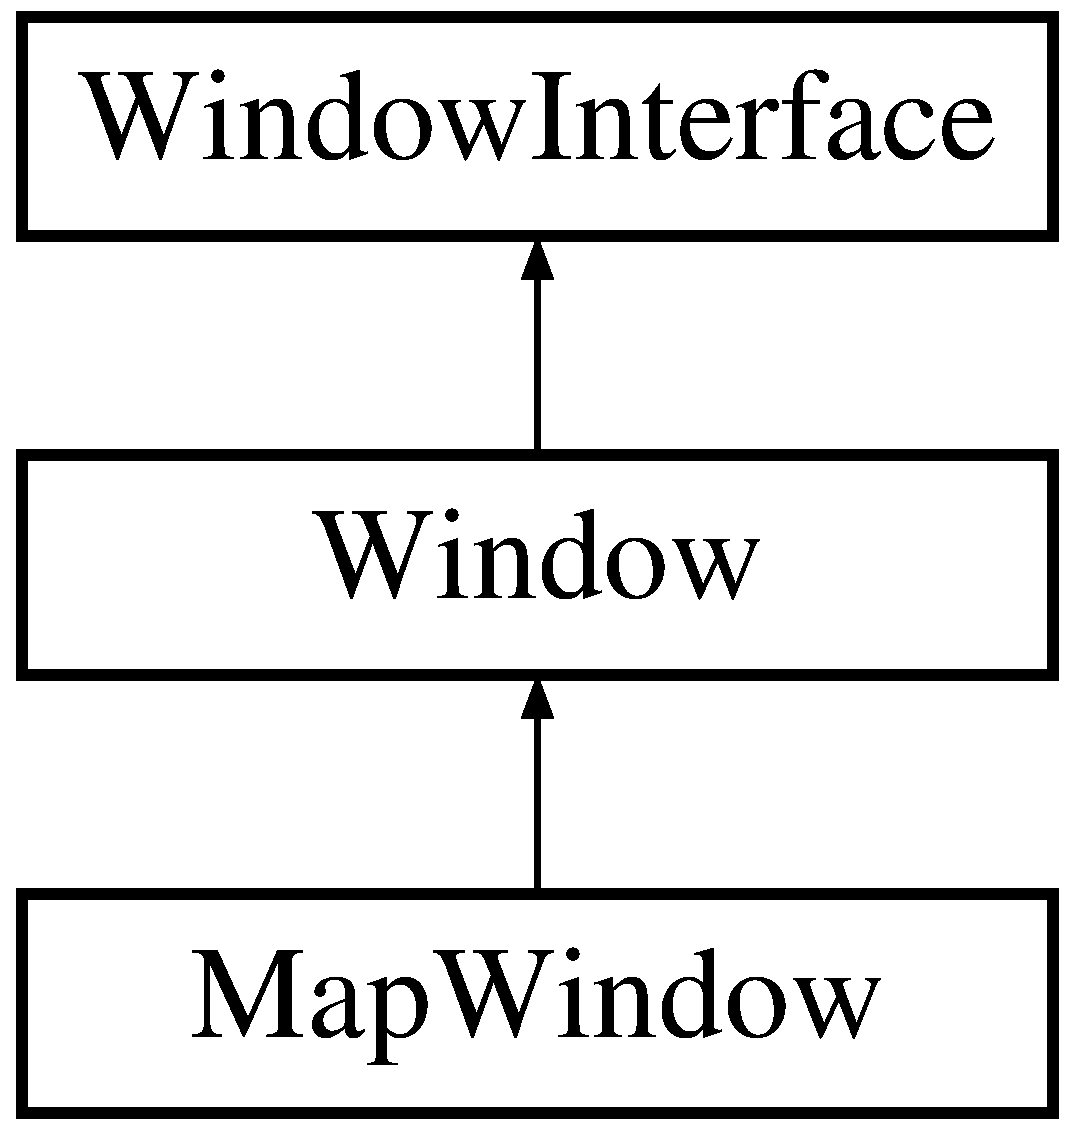
\includegraphics[height=3.000000cm]{classMapWindow}
\end{center}
\end{figure}
\subsection*{Public Member Functions}
\begin{DoxyCompactItemize}
\item 
virtual void \hyperlink{classMapWindow_affdeec7b3b899c38f16d04d170970e70}{initialise} (\hyperlink{classGameEngineInterface}{Game\-Engine\-Interface} $\ast$a\-\_\-engine)
\item 
virtual void \hyperlink{classMapWindow_a5759338c3758b2a3252ffc691958dff8}{redraw} ()
\item 
virtual void \hyperlink{classMapWindow_a289795e503a5aa600e4091f5aa8b0b8c}{key\-Down} (unsigned char key)
\item 
virtual void \hyperlink{classWindow_ae0ed7fd17df30f2d262cb684560e0469}{destroy} (void)
\item 
virtual \hyperlink{classGameEngineInterface}{Game\-Engine\-Interface} $\ast$ \hyperlink{classWindow_a55a6e31e36665bd3bcffcd844f5f0385}{get\-Engine} ()
\item 
virtual void \hyperlink{classWindow_a249f5a9513be00e59428a1df37502c63}{key\-Up} (unsigned char key)
\item 
virtual bool \hyperlink{classWindow_ac0927d0b89776959c4a95dd6737f841f}{get\-Key} (unsigned char key)
\item 
virtual void \hyperlink{classWindow_ace3bd5e6614510fce97263eccc35c0ab}{mouse\-Down} (int x, int y, int button)
\item 
virtual void \hyperlink{classWindow_a2e2c7592975405513a05a2da6a512b1c}{mouse\-Up} (int x, int y, int button)
\item 
virtual bool \hyperlink{classWindow_ab824bd52a5a055e468f7b2cc3d0b4f54}{get\-Mouse\-Button} (int button)
\item 
virtual void \hyperlink{classWindow_a1344118a395cb2fc48d4a2359372b074}{before\-Redraw} ()
\item 
virtual void \hyperlink{classWindow_a05b1d6673e37db442ecd80c54d10e6b7}{after\-Redraw} ()
\item 
virtual void \hyperlink{classWindow_a6e4274c73728009132b7e0dfad42a8de}{resize} (int width, int height)
\end{DoxyCompactItemize}
\subsection*{Static Public Attributes}
\begin{DoxyCompactItemize}
\item 
static const int \hyperlink{classWindow_a78a36ba2259fdd12ad2cf3346430fb35}{M\-A\-X\-\_\-\-B\-U\-T\-T\-O\-N\-S} = 5
\end{DoxyCompactItemize}
\subsection*{Private Member Functions}
\begin{DoxyCompactItemize}
\item 
void \hyperlink{classMapWindow_aba3e6f30eb34872bf7e01ffcb54ec94b}{draw\-Map} ()
\end{DoxyCompactItemize}


\subsection{Member Function Documentation}
\hypertarget{classWindow_a05b1d6673e37db442ecd80c54d10e6b7}{\index{Map\-Window@{Map\-Window}!after\-Redraw@{after\-Redraw}}
\index{after\-Redraw@{after\-Redraw}!MapWindow@{Map\-Window}}
\subsubsection[{after\-Redraw}]{\setlength{\rightskip}{0pt plus 5cm}void Window\-::after\-Redraw (
\begin{DoxyParamCaption}
{}
\end{DoxyParamCaption}
)\hspace{0.3cm}{\ttfamily [virtual]}, {\ttfamily [inherited]}}}\label{classWindow_a05b1d6673e37db442ecd80c54d10e6b7}


Implements \hyperlink{classWindowInterface_a37e350fc8f4a97333400c03e8544b2eb}{Window\-Interface}.

\hypertarget{classWindow_a1344118a395cb2fc48d4a2359372b074}{\index{Map\-Window@{Map\-Window}!before\-Redraw@{before\-Redraw}}
\index{before\-Redraw@{before\-Redraw}!MapWindow@{Map\-Window}}
\subsubsection[{before\-Redraw}]{\setlength{\rightskip}{0pt plus 5cm}void Window\-::before\-Redraw (
\begin{DoxyParamCaption}
{}
\end{DoxyParamCaption}
)\hspace{0.3cm}{\ttfamily [virtual]}, {\ttfamily [inherited]}}}\label{classWindow_a1344118a395cb2fc48d4a2359372b074}


Implements \hyperlink{classWindowInterface_a8aa6ce7a663628e3bd0480d4566191d2}{Window\-Interface}.

\hypertarget{classWindow_ae0ed7fd17df30f2d262cb684560e0469}{\index{Map\-Window@{Map\-Window}!destroy@{destroy}}
\index{destroy@{destroy}!MapWindow@{Map\-Window}}
\subsubsection[{destroy}]{\setlength{\rightskip}{0pt plus 5cm}void Window\-::destroy (
\begin{DoxyParamCaption}
\item[{void}]{}
\end{DoxyParamCaption}
)\hspace{0.3cm}{\ttfamily [virtual]}, {\ttfamily [inherited]}}}\label{classWindow_ae0ed7fd17df30f2d262cb684560e0469}


Implements \hyperlink{classWindowInterface_afeaed24b8e350acb196964106f2a0146}{Window\-Interface}.

\hypertarget{classMapWindow_aba3e6f30eb34872bf7e01ffcb54ec94b}{\index{Map\-Window@{Map\-Window}!draw\-Map@{draw\-Map}}
\index{draw\-Map@{draw\-Map}!MapWindow@{Map\-Window}}
\subsubsection[{draw\-Map}]{\setlength{\rightskip}{0pt plus 5cm}void Map\-Window\-::draw\-Map (
\begin{DoxyParamCaption}
{}
\end{DoxyParamCaption}
)\hspace{0.3cm}{\ttfamily [private]}}}\label{classMapWindow_aba3e6f30eb34872bf7e01ffcb54ec94b}
\hypertarget{classWindow_a55a6e31e36665bd3bcffcd844f5f0385}{\index{Map\-Window@{Map\-Window}!get\-Engine@{get\-Engine}}
\index{get\-Engine@{get\-Engine}!MapWindow@{Map\-Window}}
\subsubsection[{get\-Engine}]{\setlength{\rightskip}{0pt plus 5cm}virtual {\bf Game\-Engine\-Interface}$\ast$ Window\-::get\-Engine (
\begin{DoxyParamCaption}
{}
\end{DoxyParamCaption}
)\hspace{0.3cm}{\ttfamily [inline]}, {\ttfamily [virtual]}, {\ttfamily [inherited]}}}\label{classWindow_a55a6e31e36665bd3bcffcd844f5f0385}


Implements \hyperlink{classWindowInterface_ac5970434199b518109a95a5cb645814a}{Window\-Interface}.

\hypertarget{classWindow_ac0927d0b89776959c4a95dd6737f841f}{\index{Map\-Window@{Map\-Window}!get\-Key@{get\-Key}}
\index{get\-Key@{get\-Key}!MapWindow@{Map\-Window}}
\subsubsection[{get\-Key}]{\setlength{\rightskip}{0pt plus 5cm}virtual bool Window\-::get\-Key (
\begin{DoxyParamCaption}
\item[{unsigned char}]{key}
\end{DoxyParamCaption}
)\hspace{0.3cm}{\ttfamily [inline]}, {\ttfamily [virtual]}, {\ttfamily [inherited]}}}\label{classWindow_ac0927d0b89776959c4a95dd6737f841f}


Implements \hyperlink{classWindowInterface_ab67d23a3dee052fd5901a87518b86e4d}{Window\-Interface}.

\hypertarget{classWindow_ab824bd52a5a055e468f7b2cc3d0b4f54}{\index{Map\-Window@{Map\-Window}!get\-Mouse\-Button@{get\-Mouse\-Button}}
\index{get\-Mouse\-Button@{get\-Mouse\-Button}!MapWindow@{Map\-Window}}
\subsubsection[{get\-Mouse\-Button}]{\setlength{\rightskip}{0pt plus 5cm}bool Window\-::get\-Mouse\-Button (
\begin{DoxyParamCaption}
\item[{int}]{button}
\end{DoxyParamCaption}
)\hspace{0.3cm}{\ttfamily [virtual]}, {\ttfamily [inherited]}}}\label{classWindow_ab824bd52a5a055e468f7b2cc3d0b4f54}
\hypertarget{classMapWindow_affdeec7b3b899c38f16d04d170970e70}{\index{Map\-Window@{Map\-Window}!initialise@{initialise}}
\index{initialise@{initialise}!MapWindow@{Map\-Window}}
\subsubsection[{initialise}]{\setlength{\rightskip}{0pt plus 5cm}void Map\-Window\-::initialise (
\begin{DoxyParamCaption}
\item[{{\bf Game\-Engine\-Interface} $\ast$}]{a\-\_\-engine}
\end{DoxyParamCaption}
)\hspace{0.3cm}{\ttfamily [virtual]}}}\label{classMapWindow_affdeec7b3b899c38f16d04d170970e70}


Reimplemented from \hyperlink{classWindow_a3dcd22169bd4d40f4b35eafdea31f6dd}{Window}.

\hypertarget{classMapWindow_a289795e503a5aa600e4091f5aa8b0b8c}{\index{Map\-Window@{Map\-Window}!key\-Down@{key\-Down}}
\index{key\-Down@{key\-Down}!MapWindow@{Map\-Window}}
\subsubsection[{key\-Down}]{\setlength{\rightskip}{0pt plus 5cm}void Map\-Window\-::key\-Down (
\begin{DoxyParamCaption}
\item[{unsigned char}]{key}
\end{DoxyParamCaption}
)\hspace{0.3cm}{\ttfamily [virtual]}}}\label{classMapWindow_a289795e503a5aa600e4091f5aa8b0b8c}


Reimplemented from \hyperlink{classWindow_a25a5308909ec422bebb480c803e1233c}{Window}.

\hypertarget{classWindow_a249f5a9513be00e59428a1df37502c63}{\index{Map\-Window@{Map\-Window}!key\-Up@{key\-Up}}
\index{key\-Up@{key\-Up}!MapWindow@{Map\-Window}}
\subsubsection[{key\-Up}]{\setlength{\rightskip}{0pt plus 5cm}virtual void Window\-::key\-Up (
\begin{DoxyParamCaption}
\item[{unsigned char}]{key}
\end{DoxyParamCaption}
)\hspace{0.3cm}{\ttfamily [inline]}, {\ttfamily [virtual]}, {\ttfamily [inherited]}}}\label{classWindow_a249f5a9513be00e59428a1df37502c63}


Implements \hyperlink{classWindowInterface_aa776c5cf4ef3d93a49613e08c79cab77}{Window\-Interface}.

\hypertarget{classWindow_ace3bd5e6614510fce97263eccc35c0ab}{\index{Map\-Window@{Map\-Window}!mouse\-Down@{mouse\-Down}}
\index{mouse\-Down@{mouse\-Down}!MapWindow@{Map\-Window}}
\subsubsection[{mouse\-Down}]{\setlength{\rightskip}{0pt plus 5cm}void Window\-::mouse\-Down (
\begin{DoxyParamCaption}
\item[{int}]{x, }
\item[{int}]{y, }
\item[{int}]{button}
\end{DoxyParamCaption}
)\hspace{0.3cm}{\ttfamily [virtual]}, {\ttfamily [inherited]}}}\label{classWindow_ace3bd5e6614510fce97263eccc35c0ab}


Implements \hyperlink{classWindowInterface_a5e6ba2b8e6560e9e3b74794cfd123d59}{Window\-Interface}.

\hypertarget{classWindow_a2e2c7592975405513a05a2da6a512b1c}{\index{Map\-Window@{Map\-Window}!mouse\-Up@{mouse\-Up}}
\index{mouse\-Up@{mouse\-Up}!MapWindow@{Map\-Window}}
\subsubsection[{mouse\-Up}]{\setlength{\rightskip}{0pt plus 5cm}void Window\-::mouse\-Up (
\begin{DoxyParamCaption}
\item[{int}]{x, }
\item[{int}]{y, }
\item[{int}]{button}
\end{DoxyParamCaption}
)\hspace{0.3cm}{\ttfamily [virtual]}, {\ttfamily [inherited]}}}\label{classWindow_a2e2c7592975405513a05a2da6a512b1c}


Implements \hyperlink{classWindowInterface_a482961a40e4a07d7f7ac81fe62ee7762}{Window\-Interface}.

\hypertarget{classMapWindow_a5759338c3758b2a3252ffc691958dff8}{\index{Map\-Window@{Map\-Window}!redraw@{redraw}}
\index{redraw@{redraw}!MapWindow@{Map\-Window}}
\subsubsection[{redraw}]{\setlength{\rightskip}{0pt plus 5cm}void Map\-Window\-::redraw (
\begin{DoxyParamCaption}
{}
\end{DoxyParamCaption}
)\hspace{0.3cm}{\ttfamily [virtual]}}}\label{classMapWindow_a5759338c3758b2a3252ffc691958dff8}


Reimplemented from \hyperlink{classWindow_aa8b52b7035a78ef960c194c9bb4a7c36}{Window}.

\hypertarget{classWindow_a6e4274c73728009132b7e0dfad42a8de}{\index{Map\-Window@{Map\-Window}!resize@{resize}}
\index{resize@{resize}!MapWindow@{Map\-Window}}
\subsubsection[{resize}]{\setlength{\rightskip}{0pt plus 5cm}void Window\-::resize (
\begin{DoxyParamCaption}
\item[{int}]{width, }
\item[{int}]{height}
\end{DoxyParamCaption}
)\hspace{0.3cm}{\ttfamily [virtual]}, {\ttfamily [inherited]}}}\label{classWindow_a6e4274c73728009132b7e0dfad42a8de}


Implements \hyperlink{classWindowInterface_aa7109fc50fd3e90b0589bdd2a5e6972e}{Window\-Interface}.



\subsection{Member Data Documentation}
\hypertarget{classWindow_a78a36ba2259fdd12ad2cf3346430fb35}{\index{Map\-Window@{Map\-Window}!M\-A\-X\-\_\-\-B\-U\-T\-T\-O\-N\-S@{M\-A\-X\-\_\-\-B\-U\-T\-T\-O\-N\-S}}
\index{M\-A\-X\-\_\-\-B\-U\-T\-T\-O\-N\-S@{M\-A\-X\-\_\-\-B\-U\-T\-T\-O\-N\-S}!MapWindow@{Map\-Window}}
\subsubsection[{M\-A\-X\-\_\-\-B\-U\-T\-T\-O\-N\-S}]{\setlength{\rightskip}{0pt plus 5cm}const int Window\-::\-M\-A\-X\-\_\-\-B\-U\-T\-T\-O\-N\-S = 5\hspace{0.3cm}{\ttfamily [static]}, {\ttfamily [inherited]}}}\label{classWindow_a78a36ba2259fdd12ad2cf3346430fb35}


The documentation for this class was generated from the following files\-:\begin{DoxyCompactItemize}
\item 
\hyperlink{map__window_8h}{map\-\_\-window.\-h}\item 
\hyperlink{map__window_8cpp}{map\-\_\-window.\-cpp}\end{DoxyCompactItemize}

\hypertarget{classMoveEntityEvent}{\section{Move\-Entity\-Event Class Reference}
\label{classMoveEntityEvent}\index{Move\-Entity\-Event@{Move\-Entity\-Event}}
}


{\ttfamily \#include $<$event.\-h$>$}

Inheritance diagram for Move\-Entity\-Event\-:\begin{figure}[H]
\begin{center}
\leavevmode
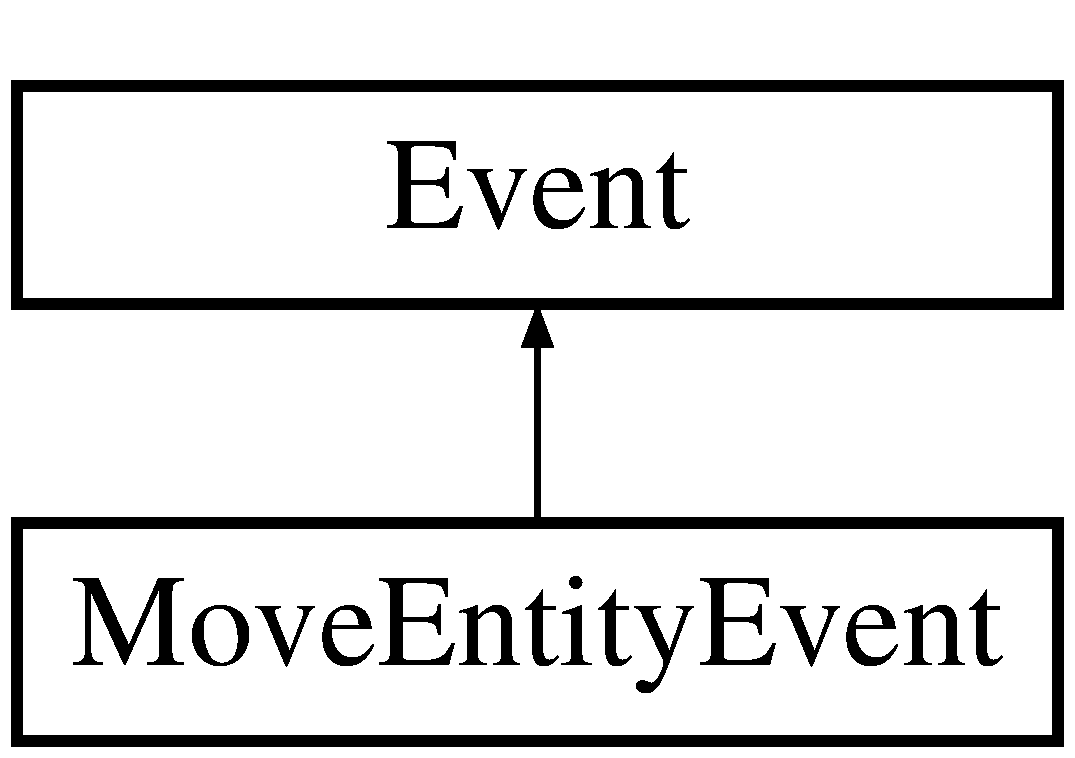
\includegraphics[height=2.000000cm]{classMoveEntityEvent}
\end{center}
\end{figure}
\subsection*{Public Types}
\begin{DoxyCompactItemize}
\item 
enum \hyperlink{classMoveEntityEvent_a7058a943643bee9164a21e62e3392807}{D\-I\-R\-E\-C\-T\-I\-O\-N} \{ \\*
\hyperlink{classMoveEntityEvent_a7058a943643bee9164a21e62e3392807a15b0c6b8a581c4dbda78987169ae5f01}{N\-O\-N\-E} = 0, 
\hyperlink{classMoveEntityEvent_a7058a943643bee9164a21e62e3392807aeef1cc5f9516b00bb914bd41a8e6b5af}{U\-P} = 1, 
\hyperlink{classMoveEntityEvent_a7058a943643bee9164a21e62e3392807ab4b62f7c78d9716e7a25b52216ab5695}{R\-I\-G\-H\-T} = 2, 
\hyperlink{classMoveEntityEvent_a7058a943643bee9164a21e62e3392807af65f060ef91fd8719accae8025ffb053}{D\-O\-W\-N} = 3, 
\\*
\hyperlink{classMoveEntityEvent_a7058a943643bee9164a21e62e3392807ae59ae25b0255eaf1ca0a083301281d7a}{L\-E\-F\-T} = 4
 \}
\end{DoxyCompactItemize}
\subsection*{Public Member Functions}
\begin{DoxyCompactItemize}
\item 
\hyperlink{classMoveEntityEvent_a93c85bd427bb61b888a5e11a6b9a9c89}{Move\-Entity\-Event} ()
\item 
\hyperlink{event_8h_a2628ea8d12e8b2563c32f05dc7fff6fa}{Event\-Type} \hyperlink{classEvent_ab0c2e30730d5859851f3126258c0126e}{get\-Type} () const 
\end{DoxyCompactItemize}
\subsection*{Public Attributes}
\begin{DoxyCompactItemize}
\item 
\hyperlink{classEntity}{Entity} $\ast$ \hyperlink{classMoveEntityEvent_aab414806813e40d92ac4c93fbf981a2b}{entity}
\item 
enum \hyperlink{classMoveEntityEvent_a7058a943643bee9164a21e62e3392807}{D\-I\-R\-E\-C\-T\-I\-O\-N} \hyperlink{classMoveEntityEvent_ac55de930d27e83d1eb92968e9c3f41eb}{direction}
\end{DoxyCompactItemize}
\subsection*{Protected Attributes}
\begin{DoxyCompactItemize}
\item 
\hyperlink{event_8h_a2628ea8d12e8b2563c32f05dc7fff6fa}{Event\-Type} \hyperlink{classEvent_a38264e3fb229dc64123dff1d5a7dcf9e}{m\-\_\-type}
\end{DoxyCompactItemize}


\subsection{Member Enumeration Documentation}
\hypertarget{classMoveEntityEvent_a7058a943643bee9164a21e62e3392807}{\index{Move\-Entity\-Event@{Move\-Entity\-Event}!D\-I\-R\-E\-C\-T\-I\-O\-N@{D\-I\-R\-E\-C\-T\-I\-O\-N}}
\index{D\-I\-R\-E\-C\-T\-I\-O\-N@{D\-I\-R\-E\-C\-T\-I\-O\-N}!MoveEntityEvent@{Move\-Entity\-Event}}
\subsubsection[{D\-I\-R\-E\-C\-T\-I\-O\-N}]{\setlength{\rightskip}{0pt plus 5cm}enum {\bf Move\-Entity\-Event\-::\-D\-I\-R\-E\-C\-T\-I\-O\-N}}}\label{classMoveEntityEvent_a7058a943643bee9164a21e62e3392807}
\begin{Desc}
\item[Enumerator]\par
\begin{description}
\index{N\-O\-N\-E@{N\-O\-N\-E}!Move\-Entity\-Event@{Move\-Entity\-Event}}\index{Move\-Entity\-Event@{Move\-Entity\-Event}!N\-O\-N\-E@{N\-O\-N\-E}}\item[{\em 
\hypertarget{classMoveEntityEvent_a7058a943643bee9164a21e62e3392807a15b0c6b8a581c4dbda78987169ae5f01}{N\-O\-N\-E}\label{classMoveEntityEvent_a7058a943643bee9164a21e62e3392807a15b0c6b8a581c4dbda78987169ae5f01}
}]\index{U\-P@{U\-P}!Move\-Entity\-Event@{Move\-Entity\-Event}}\index{Move\-Entity\-Event@{Move\-Entity\-Event}!U\-P@{U\-P}}\item[{\em 
\hypertarget{classMoveEntityEvent_a7058a943643bee9164a21e62e3392807aeef1cc5f9516b00bb914bd41a8e6b5af}{U\-P}\label{classMoveEntityEvent_a7058a943643bee9164a21e62e3392807aeef1cc5f9516b00bb914bd41a8e6b5af}
}]\index{R\-I\-G\-H\-T@{R\-I\-G\-H\-T}!Move\-Entity\-Event@{Move\-Entity\-Event}}\index{Move\-Entity\-Event@{Move\-Entity\-Event}!R\-I\-G\-H\-T@{R\-I\-G\-H\-T}}\item[{\em 
\hypertarget{classMoveEntityEvent_a7058a943643bee9164a21e62e3392807ab4b62f7c78d9716e7a25b52216ab5695}{R\-I\-G\-H\-T}\label{classMoveEntityEvent_a7058a943643bee9164a21e62e3392807ab4b62f7c78d9716e7a25b52216ab5695}
}]\index{D\-O\-W\-N@{D\-O\-W\-N}!Move\-Entity\-Event@{Move\-Entity\-Event}}\index{Move\-Entity\-Event@{Move\-Entity\-Event}!D\-O\-W\-N@{D\-O\-W\-N}}\item[{\em 
\hypertarget{classMoveEntityEvent_a7058a943643bee9164a21e62e3392807af65f060ef91fd8719accae8025ffb053}{D\-O\-W\-N}\label{classMoveEntityEvent_a7058a943643bee9164a21e62e3392807af65f060ef91fd8719accae8025ffb053}
}]\index{L\-E\-F\-T@{L\-E\-F\-T}!Move\-Entity\-Event@{Move\-Entity\-Event}}\index{Move\-Entity\-Event@{Move\-Entity\-Event}!L\-E\-F\-T@{L\-E\-F\-T}}\item[{\em 
\hypertarget{classMoveEntityEvent_a7058a943643bee9164a21e62e3392807ae59ae25b0255eaf1ca0a083301281d7a}{L\-E\-F\-T}\label{classMoveEntityEvent_a7058a943643bee9164a21e62e3392807ae59ae25b0255eaf1ca0a083301281d7a}
}]\end{description}
\end{Desc}


\subsection{Constructor \& Destructor Documentation}
\hypertarget{classMoveEntityEvent_a93c85bd427bb61b888a5e11a6b9a9c89}{\index{Move\-Entity\-Event@{Move\-Entity\-Event}!Move\-Entity\-Event@{Move\-Entity\-Event}}
\index{Move\-Entity\-Event@{Move\-Entity\-Event}!MoveEntityEvent@{Move\-Entity\-Event}}
\subsubsection[{Move\-Entity\-Event}]{\setlength{\rightskip}{0pt plus 5cm}Move\-Entity\-Event\-::\-Move\-Entity\-Event (
\begin{DoxyParamCaption}
{}
\end{DoxyParamCaption}
)\hspace{0.3cm}{\ttfamily [inline]}}}\label{classMoveEntityEvent_a93c85bd427bb61b888a5e11a6b9a9c89}


\subsection{Member Function Documentation}
\hypertarget{classEvent_ab0c2e30730d5859851f3126258c0126e}{\index{Move\-Entity\-Event@{Move\-Entity\-Event}!get\-Type@{get\-Type}}
\index{get\-Type@{get\-Type}!MoveEntityEvent@{Move\-Entity\-Event}}
\subsubsection[{get\-Type}]{\setlength{\rightskip}{0pt plus 5cm}{\bf Event\-Type} Event\-::get\-Type (
\begin{DoxyParamCaption}
{}
\end{DoxyParamCaption}
) const\hspace{0.3cm}{\ttfamily [inline]}, {\ttfamily [inherited]}}}\label{classEvent_ab0c2e30730d5859851f3126258c0126e}


\subsection{Member Data Documentation}
\hypertarget{classMoveEntityEvent_ac55de930d27e83d1eb92968e9c3f41eb}{\index{Move\-Entity\-Event@{Move\-Entity\-Event}!direction@{direction}}
\index{direction@{direction}!MoveEntityEvent@{Move\-Entity\-Event}}
\subsubsection[{direction}]{\setlength{\rightskip}{0pt plus 5cm}enum {\bf D\-I\-R\-E\-C\-T\-I\-O\-N} Move\-Entity\-Event\-::direction}}\label{classMoveEntityEvent_ac55de930d27e83d1eb92968e9c3f41eb}
\hypertarget{classMoveEntityEvent_aab414806813e40d92ac4c93fbf981a2b}{\index{Move\-Entity\-Event@{Move\-Entity\-Event}!entity@{entity}}
\index{entity@{entity}!MoveEntityEvent@{Move\-Entity\-Event}}
\subsubsection[{entity}]{\setlength{\rightskip}{0pt plus 5cm}{\bf Entity}$\ast$ Move\-Entity\-Event\-::entity}}\label{classMoveEntityEvent_aab414806813e40d92ac4c93fbf981a2b}
\hypertarget{classEvent_a38264e3fb229dc64123dff1d5a7dcf9e}{\index{Move\-Entity\-Event@{Move\-Entity\-Event}!m\-\_\-type@{m\-\_\-type}}
\index{m\-\_\-type@{m\-\_\-type}!MoveEntityEvent@{Move\-Entity\-Event}}
\subsubsection[{m\-\_\-type}]{\setlength{\rightskip}{0pt plus 5cm}{\bf Event\-Type} Event\-::m\-\_\-type\hspace{0.3cm}{\ttfamily [protected]}, {\ttfamily [inherited]}}}\label{classEvent_a38264e3fb229dc64123dff1d5a7dcf9e}


The documentation for this class was generated from the following file\-:\begin{DoxyCompactItemize}
\item 
\hyperlink{event_8h}{event.\-h}\end{DoxyCompactItemize}

\hypertarget{classMovementSystem}{\section{Movement\-System Class Reference}
\label{classMovementSystem}\index{Movement\-System@{Movement\-System}}
}


{\ttfamily \#include $<$movement\-\_\-system.\-h$>$}

Inheritance diagram for Movement\-System\-:\begin{figure}[H]
\begin{center}
\leavevmode
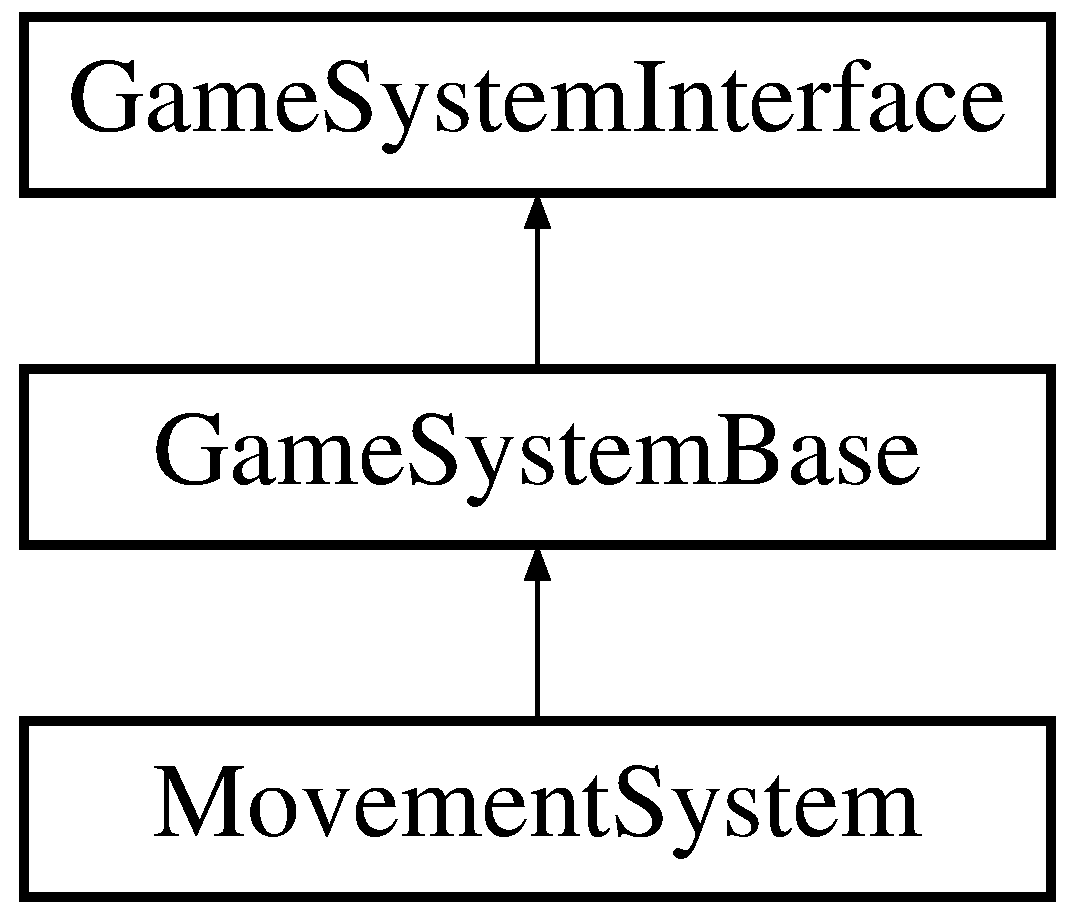
\includegraphics[height=3.000000cm]{classMovementSystem}
\end{center}
\end{figure}
\subsection*{Public Member Functions}
\begin{DoxyCompactItemize}
\item 
virtual \hyperlink{classMovementSystem_a51ef4a49db0f68096e421b3430954716}{$\sim$\-Movement\-System} ()
\item 
virtual void \hyperlink{classMovementSystem_ac2c594a6deb6349a376cd72f189971a3}{handle\-Event} (const \hyperlink{classEvent}{Event} $\ast$event)
\item 
virtual void \hyperlink{classGameSystemBase_a55b4fc27cbfccd3c724c2e5984d78625}{initialise} (\hyperlink{classGameEngineInterface}{Game\-Engine\-Interface} $\ast$engine)
\item 
virtual \hyperlink{classGameEngineInterface}{Game\-Engine\-Interface} $\ast$ \hyperlink{classGameSystemBase_a1954c5a1c79963554805bc25b2cd6072}{get\-Engine\-Ref} ()
\item 
virtual void \hyperlink{classGameSystemBase_a039d3086ac7fe50abdb110b569520d69}{update} ()
\item 
virtual std\-::vector$<$ \hyperlink{classEntity}{Entity} $\ast$ $>$ \hyperlink{classGameSystemBase_aae270a88f1077a091e6033514b889abd}{find\-Entities\-Near} (unsigned int x, unsigned int y, unsigned radius)
\item 
virtual std\-::vector$<$ \hyperlink{classEntity}{Entity} $\ast$ $>$ \hyperlink{classGameSystemBase_a7aa9912fc078d990dbfb480e411bd3bc}{find\-Entities\-At} (unsigned int x, unsigned int y)
\item 
virtual std\-::vector$<$ \hyperlink{classEntity}{Entity} $\ast$ $>$ \hyperlink{classGameSystemBase_a44456ef40ac565b9d6b65f3b1531a4ef}{find\-Entities\-To\-The} (\hyperlink{classMoveEntityEvent_a7058a943643bee9164a21e62e3392807}{Move\-Entity\-Event\-::\-D\-I\-R\-E\-C\-T\-I\-O\-N} a\-\_\-direction, \hyperlink{classEntity}{Entity} $\ast$a\-\_\-entity)
\end{DoxyCompactItemize}
\subsection*{Protected Attributes}
\begin{DoxyCompactItemize}
\item 
\hyperlink{classGameEngineInterface}{Game\-Engine\-Interface} $\ast$ \hyperlink{classGameSystemBase_aa9044eb22399f0c0ddd8f049738c62e5}{m\-\_\-engine}
\end{DoxyCompactItemize}


\subsection{Constructor \& Destructor Documentation}
\hypertarget{classMovementSystem_a51ef4a49db0f68096e421b3430954716}{\index{Movement\-System@{Movement\-System}!$\sim$\-Movement\-System@{$\sim$\-Movement\-System}}
\index{$\sim$\-Movement\-System@{$\sim$\-Movement\-System}!MovementSystem@{Movement\-System}}
\subsubsection[{$\sim$\-Movement\-System}]{\setlength{\rightskip}{0pt plus 5cm}virtual Movement\-System\-::$\sim$\-Movement\-System (
\begin{DoxyParamCaption}
{}
\end{DoxyParamCaption}
)\hspace{0.3cm}{\ttfamily [inline]}, {\ttfamily [virtual]}}}\label{classMovementSystem_a51ef4a49db0f68096e421b3430954716}


\subsection{Member Function Documentation}
\hypertarget{classGameSystemBase_a7aa9912fc078d990dbfb480e411bd3bc}{\index{Movement\-System@{Movement\-System}!find\-Entities\-At@{find\-Entities\-At}}
\index{find\-Entities\-At@{find\-Entities\-At}!MovementSystem@{Movement\-System}}
\subsubsection[{find\-Entities\-At}]{\setlength{\rightskip}{0pt plus 5cm}std\-::vector$<$ {\bf Entity} $\ast$ $>$ Game\-System\-Base\-::find\-Entities\-At (
\begin{DoxyParamCaption}
\item[{unsigned int}]{x, }
\item[{unsigned int}]{y}
\end{DoxyParamCaption}
)\hspace{0.3cm}{\ttfamily [virtual]}, {\ttfamily [inherited]}}}\label{classGameSystemBase_a7aa9912fc078d990dbfb480e411bd3bc}
\hypertarget{classGameSystemBase_aae270a88f1077a091e6033514b889abd}{\index{Movement\-System@{Movement\-System}!find\-Entities\-Near@{find\-Entities\-Near}}
\index{find\-Entities\-Near@{find\-Entities\-Near}!MovementSystem@{Movement\-System}}
\subsubsection[{find\-Entities\-Near}]{\setlength{\rightskip}{0pt plus 5cm}std\-::vector$<$ {\bf Entity} $\ast$ $>$ Game\-System\-Base\-::find\-Entities\-Near (
\begin{DoxyParamCaption}
\item[{unsigned int}]{x, }
\item[{unsigned int}]{y, }
\item[{unsigned}]{radius}
\end{DoxyParamCaption}
)\hspace{0.3cm}{\ttfamily [virtual]}, {\ttfamily [inherited]}}}\label{classGameSystemBase_aae270a88f1077a091e6033514b889abd}
\hypertarget{classGameSystemBase_a44456ef40ac565b9d6b65f3b1531a4ef}{\index{Movement\-System@{Movement\-System}!find\-Entities\-To\-The@{find\-Entities\-To\-The}}
\index{find\-Entities\-To\-The@{find\-Entities\-To\-The}!MovementSystem@{Movement\-System}}
\subsubsection[{find\-Entities\-To\-The}]{\setlength{\rightskip}{0pt plus 5cm}std\-::vector$<$ {\bf Entity} $\ast$ $>$ Game\-System\-Base\-::find\-Entities\-To\-The (
\begin{DoxyParamCaption}
\item[{{\bf Move\-Entity\-Event\-::\-D\-I\-R\-E\-C\-T\-I\-O\-N}}]{a\-\_\-direction, }
\item[{{\bf Entity} $\ast$}]{a\-\_\-entity}
\end{DoxyParamCaption}
)\hspace{0.3cm}{\ttfamily [virtual]}, {\ttfamily [inherited]}}}\label{classGameSystemBase_a44456ef40ac565b9d6b65f3b1531a4ef}
\hypertarget{classGameSystemBase_a1954c5a1c79963554805bc25b2cd6072}{\index{Movement\-System@{Movement\-System}!get\-Engine\-Ref@{get\-Engine\-Ref}}
\index{get\-Engine\-Ref@{get\-Engine\-Ref}!MovementSystem@{Movement\-System}}
\subsubsection[{get\-Engine\-Ref}]{\setlength{\rightskip}{0pt plus 5cm}virtual {\bf Game\-Engine\-Interface}$\ast$ Game\-System\-Base\-::get\-Engine\-Ref (
\begin{DoxyParamCaption}
{}
\end{DoxyParamCaption}
)\hspace{0.3cm}{\ttfamily [inline]}, {\ttfamily [virtual]}, {\ttfamily [inherited]}}}\label{classGameSystemBase_a1954c5a1c79963554805bc25b2cd6072}
\hypertarget{classMovementSystem_ac2c594a6deb6349a376cd72f189971a3}{\index{Movement\-System@{Movement\-System}!handle\-Event@{handle\-Event}}
\index{handle\-Event@{handle\-Event}!MovementSystem@{Movement\-System}}
\subsubsection[{handle\-Event}]{\setlength{\rightskip}{0pt plus 5cm}void Movement\-System\-::handle\-Event (
\begin{DoxyParamCaption}
\item[{const {\bf Event} $\ast$}]{event}
\end{DoxyParamCaption}
)\hspace{0.3cm}{\ttfamily [virtual]}}}\label{classMovementSystem_ac2c594a6deb6349a376cd72f189971a3}


Reimplemented from \hyperlink{classGameSystemBase_a007b3ece290b1ad0dc3e397c5264d44d}{Game\-System\-Base}.

\hypertarget{classGameSystemBase_a55b4fc27cbfccd3c724c2e5984d78625}{\index{Movement\-System@{Movement\-System}!initialise@{initialise}}
\index{initialise@{initialise}!MovementSystem@{Movement\-System}}
\subsubsection[{initialise}]{\setlength{\rightskip}{0pt plus 5cm}virtual void Game\-System\-Base\-::initialise (
\begin{DoxyParamCaption}
\item[{{\bf Game\-Engine\-Interface} $\ast$}]{engine}
\end{DoxyParamCaption}
)\hspace{0.3cm}{\ttfamily [inline]}, {\ttfamily [virtual]}, {\ttfamily [inherited]}}}\label{classGameSystemBase_a55b4fc27cbfccd3c724c2e5984d78625}


Implements \hyperlink{classGameSystemInterface_a29079ef1f35027150b751c3fcb025091}{Game\-System\-Interface}.

\hypertarget{classGameSystemBase_a039d3086ac7fe50abdb110b569520d69}{\index{Movement\-System@{Movement\-System}!update@{update}}
\index{update@{update}!MovementSystem@{Movement\-System}}
\subsubsection[{update}]{\setlength{\rightskip}{0pt plus 5cm}virtual void Game\-System\-Base\-::update (
\begin{DoxyParamCaption}
{}
\end{DoxyParamCaption}
)\hspace{0.3cm}{\ttfamily [inline]}, {\ttfamily [virtual]}, {\ttfamily [inherited]}}}\label{classGameSystemBase_a039d3086ac7fe50abdb110b569520d69}


Implements \hyperlink{classGameSystemInterface_a531f5e7c6ca9881a67932cc4fded0a2e}{Game\-System\-Interface}.



Reimplemented in \hyperlink{classNpcSystem_a88d87a8ec981e5cf1f4ed4340123a9d8}{Npc\-System}.



\subsection{Member Data Documentation}
\hypertarget{classGameSystemBase_aa9044eb22399f0c0ddd8f049738c62e5}{\index{Movement\-System@{Movement\-System}!m\-\_\-engine@{m\-\_\-engine}}
\index{m\-\_\-engine@{m\-\_\-engine}!MovementSystem@{Movement\-System}}
\subsubsection[{m\-\_\-engine}]{\setlength{\rightskip}{0pt plus 5cm}{\bf Game\-Engine\-Interface}$\ast$ Game\-System\-Base\-::m\-\_\-engine\hspace{0.3cm}{\ttfamily [protected]}, {\ttfamily [inherited]}}}\label{classGameSystemBase_aa9044eb22399f0c0ddd8f049738c62e5}


The documentation for this class was generated from the following files\-:\begin{DoxyCompactItemize}
\item 
\hyperlink{movement__system_8h}{movement\-\_\-system.\-h}\item 
\hyperlink{movement__system_8cpp}{movement\-\_\-system.\-cpp}\end{DoxyCompactItemize}

\hypertarget{classNpcSystem}{\section{Npc\-System Class Reference}
\label{classNpcSystem}\index{Npc\-System@{Npc\-System}}
}


{\ttfamily \#include $<$npc\-\_\-system.\-h$>$}

Inheritance diagram for Npc\-System\-:\begin{figure}[H]
\begin{center}
\leavevmode
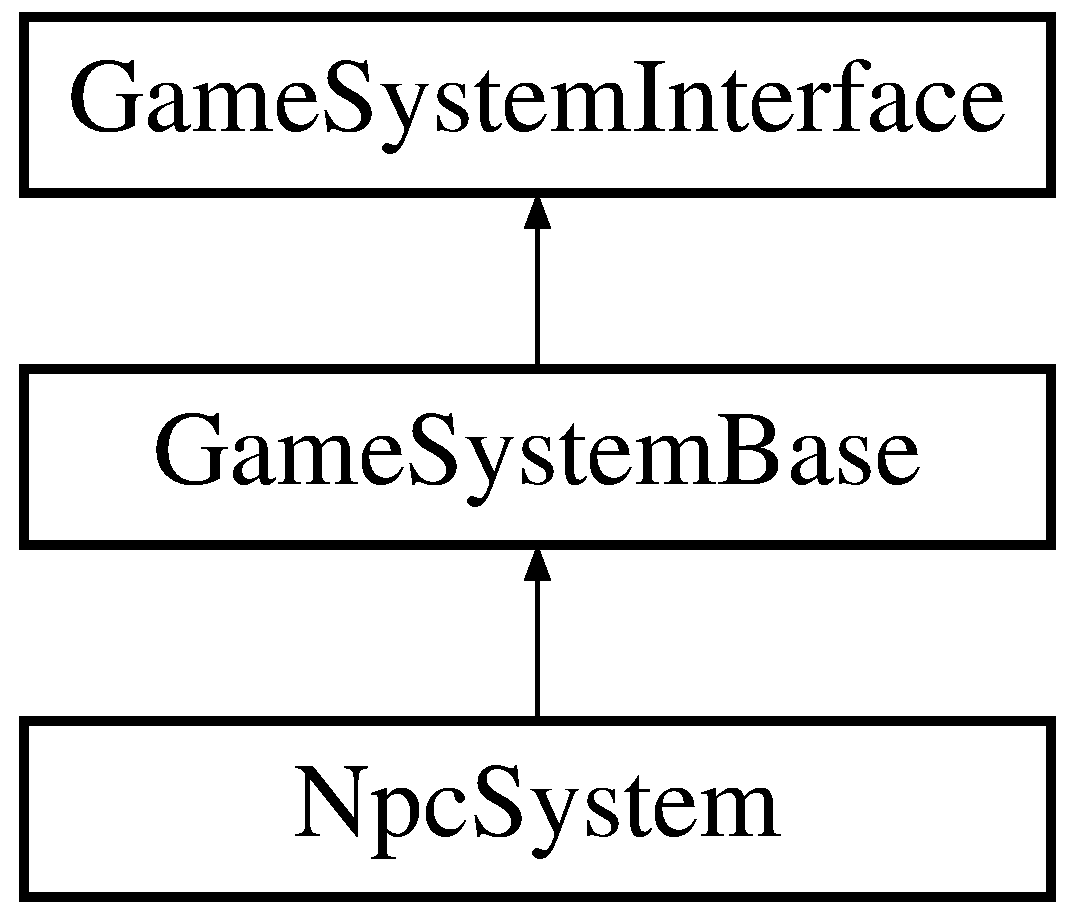
\includegraphics[height=3.000000cm]{classNpcSystem}
\end{center}
\end{figure}
\subsection*{Public Member Functions}
\begin{DoxyCompactItemize}
\item 
virtual void \hyperlink{classNpcSystem_ad4c89f0e50944fc2f9dd7206411ced53}{handle\-Event} (const \hyperlink{classEvent}{Event} $\ast$event)
\item 
virtual void \hyperlink{classNpcSystem_a88d87a8ec981e5cf1f4ed4340123a9d8}{update} ()
\item 
virtual void \hyperlink{classGameSystemBase_a55b4fc27cbfccd3c724c2e5984d78625}{initialise} (\hyperlink{classGameEngineInterface}{Game\-Engine\-Interface} $\ast$engine)
\item 
virtual \hyperlink{classGameEngineInterface}{Game\-Engine\-Interface} $\ast$ \hyperlink{classGameSystemBase_a1954c5a1c79963554805bc25b2cd6072}{get\-Engine\-Ref} ()
\item 
virtual std\-::vector$<$ \hyperlink{classEntity}{Entity} $\ast$ $>$ \hyperlink{classGameSystemBase_aae270a88f1077a091e6033514b889abd}{find\-Entities\-Near} (unsigned int x, unsigned int y, unsigned radius)
\item 
virtual std\-::vector$<$ \hyperlink{classEntity}{Entity} $\ast$ $>$ \hyperlink{classGameSystemBase_a7aa9912fc078d990dbfb480e411bd3bc}{find\-Entities\-At} (unsigned int x, unsigned int y)
\item 
virtual std\-::vector$<$ \hyperlink{classEntity}{Entity} $\ast$ $>$ \hyperlink{classGameSystemBase_a44456ef40ac565b9d6b65f3b1531a4ef}{find\-Entities\-To\-The} (\hyperlink{classMoveEntityEvent_a7058a943643bee9164a21e62e3392807}{Move\-Entity\-Event\-::\-D\-I\-R\-E\-C\-T\-I\-O\-N} a\-\_\-direction, \hyperlink{classEntity}{Entity} $\ast$a\-\_\-entity)
\end{DoxyCompactItemize}
\subsection*{Protected Attributes}
\begin{DoxyCompactItemize}
\item 
\hyperlink{classGameEngineInterface}{Game\-Engine\-Interface} $\ast$ \hyperlink{classGameSystemBase_aa9044eb22399f0c0ddd8f049738c62e5}{m\-\_\-engine}
\end{DoxyCompactItemize}
\subsection*{Private Member Functions}
\begin{DoxyCompactItemize}
\item 
\hyperlink{classMoveEntityEvent_a7058a943643bee9164a21e62e3392807}{Move\-Entity\-Event\-::\-D\-I\-R\-E\-C\-T\-I\-O\-N} \hyperlink{classNpcSystem_a3ece27c9f3e3d3084c879ba506e691d5}{get\-Random\-Direction} ()
\end{DoxyCompactItemize}


\subsection{Member Function Documentation}
\hypertarget{classGameSystemBase_a7aa9912fc078d990dbfb480e411bd3bc}{\index{Npc\-System@{Npc\-System}!find\-Entities\-At@{find\-Entities\-At}}
\index{find\-Entities\-At@{find\-Entities\-At}!NpcSystem@{Npc\-System}}
\subsubsection[{find\-Entities\-At}]{\setlength{\rightskip}{0pt plus 5cm}std\-::vector$<$ {\bf Entity} $\ast$ $>$ Game\-System\-Base\-::find\-Entities\-At (
\begin{DoxyParamCaption}
\item[{unsigned int}]{x, }
\item[{unsigned int}]{y}
\end{DoxyParamCaption}
)\hspace{0.3cm}{\ttfamily [virtual]}, {\ttfamily [inherited]}}}\label{classGameSystemBase_a7aa9912fc078d990dbfb480e411bd3bc}
\hypertarget{classGameSystemBase_aae270a88f1077a091e6033514b889abd}{\index{Npc\-System@{Npc\-System}!find\-Entities\-Near@{find\-Entities\-Near}}
\index{find\-Entities\-Near@{find\-Entities\-Near}!NpcSystem@{Npc\-System}}
\subsubsection[{find\-Entities\-Near}]{\setlength{\rightskip}{0pt plus 5cm}std\-::vector$<$ {\bf Entity} $\ast$ $>$ Game\-System\-Base\-::find\-Entities\-Near (
\begin{DoxyParamCaption}
\item[{unsigned int}]{x, }
\item[{unsigned int}]{y, }
\item[{unsigned}]{radius}
\end{DoxyParamCaption}
)\hspace{0.3cm}{\ttfamily [virtual]}, {\ttfamily [inherited]}}}\label{classGameSystemBase_aae270a88f1077a091e6033514b889abd}
\hypertarget{classGameSystemBase_a44456ef40ac565b9d6b65f3b1531a4ef}{\index{Npc\-System@{Npc\-System}!find\-Entities\-To\-The@{find\-Entities\-To\-The}}
\index{find\-Entities\-To\-The@{find\-Entities\-To\-The}!NpcSystem@{Npc\-System}}
\subsubsection[{find\-Entities\-To\-The}]{\setlength{\rightskip}{0pt plus 5cm}std\-::vector$<$ {\bf Entity} $\ast$ $>$ Game\-System\-Base\-::find\-Entities\-To\-The (
\begin{DoxyParamCaption}
\item[{{\bf Move\-Entity\-Event\-::\-D\-I\-R\-E\-C\-T\-I\-O\-N}}]{a\-\_\-direction, }
\item[{{\bf Entity} $\ast$}]{a\-\_\-entity}
\end{DoxyParamCaption}
)\hspace{0.3cm}{\ttfamily [virtual]}, {\ttfamily [inherited]}}}\label{classGameSystemBase_a44456ef40ac565b9d6b65f3b1531a4ef}
\hypertarget{classGameSystemBase_a1954c5a1c79963554805bc25b2cd6072}{\index{Npc\-System@{Npc\-System}!get\-Engine\-Ref@{get\-Engine\-Ref}}
\index{get\-Engine\-Ref@{get\-Engine\-Ref}!NpcSystem@{Npc\-System}}
\subsubsection[{get\-Engine\-Ref}]{\setlength{\rightskip}{0pt plus 5cm}virtual {\bf Game\-Engine\-Interface}$\ast$ Game\-System\-Base\-::get\-Engine\-Ref (
\begin{DoxyParamCaption}
{}
\end{DoxyParamCaption}
)\hspace{0.3cm}{\ttfamily [inline]}, {\ttfamily [virtual]}, {\ttfamily [inherited]}}}\label{classGameSystemBase_a1954c5a1c79963554805bc25b2cd6072}
\hypertarget{classNpcSystem_a3ece27c9f3e3d3084c879ba506e691d5}{\index{Npc\-System@{Npc\-System}!get\-Random\-Direction@{get\-Random\-Direction}}
\index{get\-Random\-Direction@{get\-Random\-Direction}!NpcSystem@{Npc\-System}}
\subsubsection[{get\-Random\-Direction}]{\setlength{\rightskip}{0pt plus 5cm}{\bf Move\-Entity\-Event\-::\-D\-I\-R\-E\-C\-T\-I\-O\-N} Npc\-System\-::get\-Random\-Direction (
\begin{DoxyParamCaption}
{}
\end{DoxyParamCaption}
)\hspace{0.3cm}{\ttfamily [private]}}}\label{classNpcSystem_a3ece27c9f3e3d3084c879ba506e691d5}
\hypertarget{classNpcSystem_ad4c89f0e50944fc2f9dd7206411ced53}{\index{Npc\-System@{Npc\-System}!handle\-Event@{handle\-Event}}
\index{handle\-Event@{handle\-Event}!NpcSystem@{Npc\-System}}
\subsubsection[{handle\-Event}]{\setlength{\rightskip}{0pt plus 5cm}void Npc\-System\-::handle\-Event (
\begin{DoxyParamCaption}
\item[{const {\bf Event} $\ast$}]{event}
\end{DoxyParamCaption}
)\hspace{0.3cm}{\ttfamily [virtual]}}}\label{classNpcSystem_ad4c89f0e50944fc2f9dd7206411ced53}


Reimplemented from \hyperlink{classGameSystemBase_a007b3ece290b1ad0dc3e397c5264d44d}{Game\-System\-Base}.

\hypertarget{classGameSystemBase_a55b4fc27cbfccd3c724c2e5984d78625}{\index{Npc\-System@{Npc\-System}!initialise@{initialise}}
\index{initialise@{initialise}!NpcSystem@{Npc\-System}}
\subsubsection[{initialise}]{\setlength{\rightskip}{0pt plus 5cm}virtual void Game\-System\-Base\-::initialise (
\begin{DoxyParamCaption}
\item[{{\bf Game\-Engine\-Interface} $\ast$}]{engine}
\end{DoxyParamCaption}
)\hspace{0.3cm}{\ttfamily [inline]}, {\ttfamily [virtual]}, {\ttfamily [inherited]}}}\label{classGameSystemBase_a55b4fc27cbfccd3c724c2e5984d78625}


Implements \hyperlink{classGameSystemInterface_a29079ef1f35027150b751c3fcb025091}{Game\-System\-Interface}.

\hypertarget{classNpcSystem_a88d87a8ec981e5cf1f4ed4340123a9d8}{\index{Npc\-System@{Npc\-System}!update@{update}}
\index{update@{update}!NpcSystem@{Npc\-System}}
\subsubsection[{update}]{\setlength{\rightskip}{0pt plus 5cm}void Npc\-System\-::update (
\begin{DoxyParamCaption}
{}
\end{DoxyParamCaption}
)\hspace{0.3cm}{\ttfamily [virtual]}}}\label{classNpcSystem_a88d87a8ec981e5cf1f4ed4340123a9d8}


Reimplemented from \hyperlink{classGameSystemBase_a039d3086ac7fe50abdb110b569520d69}{Game\-System\-Base}.



\subsection{Member Data Documentation}
\hypertarget{classGameSystemBase_aa9044eb22399f0c0ddd8f049738c62e5}{\index{Npc\-System@{Npc\-System}!m\-\_\-engine@{m\-\_\-engine}}
\index{m\-\_\-engine@{m\-\_\-engine}!NpcSystem@{Npc\-System}}
\subsubsection[{m\-\_\-engine}]{\setlength{\rightskip}{0pt plus 5cm}{\bf Game\-Engine\-Interface}$\ast$ Game\-System\-Base\-::m\-\_\-engine\hspace{0.3cm}{\ttfamily [protected]}, {\ttfamily [inherited]}}}\label{classGameSystemBase_aa9044eb22399f0c0ddd8f049738c62e5}


The documentation for this class was generated from the following files\-:\begin{DoxyCompactItemize}
\item 
\hyperlink{npc__system_8h}{npc\-\_\-system.\-h}\item 
\hyperlink{npc__system_8cpp}{npc\-\_\-system.\-cpp}\end{DoxyCompactItemize}

\hypertarget{classRemoveEntityEvent}{\section{Remove\-Entity\-Event Class Reference}
\label{classRemoveEntityEvent}\index{Remove\-Entity\-Event@{Remove\-Entity\-Event}}
}


{\ttfamily \#include $<$event.\-h$>$}

Inheritance diagram for Remove\-Entity\-Event\-:\begin{figure}[H]
\begin{center}
\leavevmode
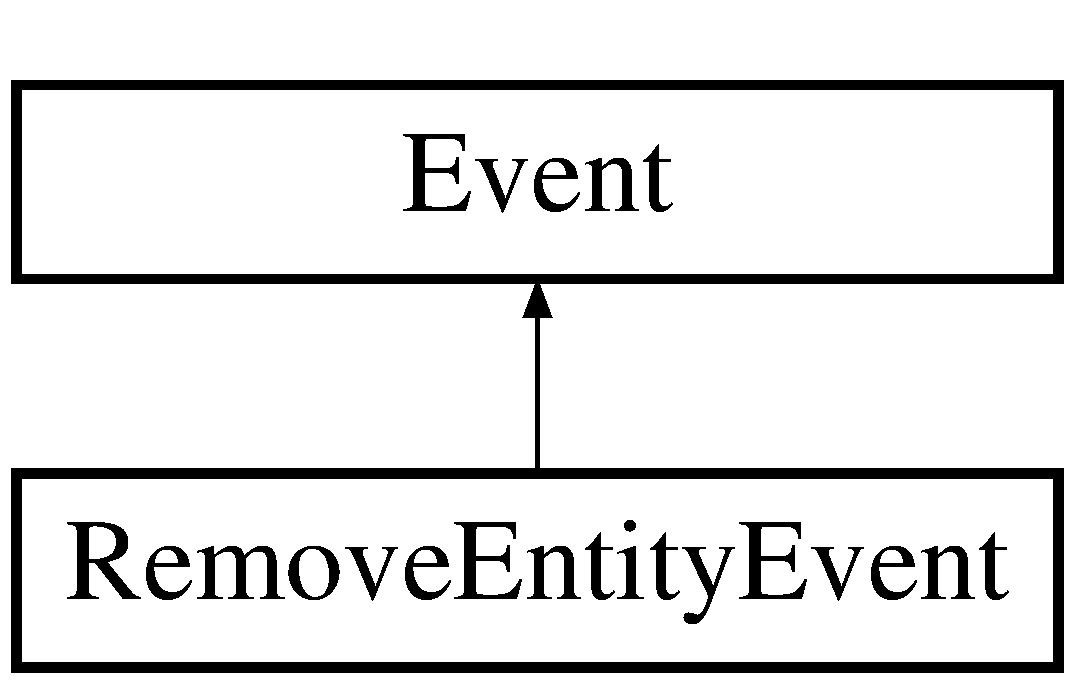
\includegraphics[height=2.000000cm]{classRemoveEntityEvent}
\end{center}
\end{figure}
\subsection*{Public Member Functions}
\begin{DoxyCompactItemize}
\item 
\hyperlink{classRemoveEntityEvent_a81436e49e915dde130239bef999e09a8}{Remove\-Entity\-Event} ()
\item 
\hyperlink{event_8h_a2628ea8d12e8b2563c32f05dc7fff6fa}{Event\-Type} \hyperlink{classEvent_ab0c2e30730d5859851f3126258c0126e}{get\-Type} () const 
\end{DoxyCompactItemize}
\subsection*{Public Attributes}
\begin{DoxyCompactItemize}
\item 
\hyperlink{classEntity}{Entity} $\ast$ \hyperlink{classRemoveEntityEvent_ad2b1c7ba91298806b66d78a814882d2a}{entity}
\end{DoxyCompactItemize}
\subsection*{Protected Attributes}
\begin{DoxyCompactItemize}
\item 
\hyperlink{event_8h_a2628ea8d12e8b2563c32f05dc7fff6fa}{Event\-Type} \hyperlink{classEvent_a38264e3fb229dc64123dff1d5a7dcf9e}{m\-\_\-type}
\end{DoxyCompactItemize}


\subsection{Constructor \& Destructor Documentation}
\hypertarget{classRemoveEntityEvent_a81436e49e915dde130239bef999e09a8}{\index{Remove\-Entity\-Event@{Remove\-Entity\-Event}!Remove\-Entity\-Event@{Remove\-Entity\-Event}}
\index{Remove\-Entity\-Event@{Remove\-Entity\-Event}!RemoveEntityEvent@{Remove\-Entity\-Event}}
\subsubsection[{Remove\-Entity\-Event}]{\setlength{\rightskip}{0pt plus 5cm}Remove\-Entity\-Event\-::\-Remove\-Entity\-Event (
\begin{DoxyParamCaption}
{}
\end{DoxyParamCaption}
)\hspace{0.3cm}{\ttfamily [inline]}}}\label{classRemoveEntityEvent_a81436e49e915dde130239bef999e09a8}


\subsection{Member Function Documentation}
\hypertarget{classEvent_ab0c2e30730d5859851f3126258c0126e}{\index{Remove\-Entity\-Event@{Remove\-Entity\-Event}!get\-Type@{get\-Type}}
\index{get\-Type@{get\-Type}!RemoveEntityEvent@{Remove\-Entity\-Event}}
\subsubsection[{get\-Type}]{\setlength{\rightskip}{0pt plus 5cm}{\bf Event\-Type} Event\-::get\-Type (
\begin{DoxyParamCaption}
{}
\end{DoxyParamCaption}
) const\hspace{0.3cm}{\ttfamily [inline]}, {\ttfamily [inherited]}}}\label{classEvent_ab0c2e30730d5859851f3126258c0126e}


\subsection{Member Data Documentation}
\hypertarget{classRemoveEntityEvent_ad2b1c7ba91298806b66d78a814882d2a}{\index{Remove\-Entity\-Event@{Remove\-Entity\-Event}!entity@{entity}}
\index{entity@{entity}!RemoveEntityEvent@{Remove\-Entity\-Event}}
\subsubsection[{entity}]{\setlength{\rightskip}{0pt plus 5cm}{\bf Entity}$\ast$ Remove\-Entity\-Event\-::entity}}\label{classRemoveEntityEvent_ad2b1c7ba91298806b66d78a814882d2a}
\hypertarget{classEvent_a38264e3fb229dc64123dff1d5a7dcf9e}{\index{Remove\-Entity\-Event@{Remove\-Entity\-Event}!m\-\_\-type@{m\-\_\-type}}
\index{m\-\_\-type@{m\-\_\-type}!RemoveEntityEvent@{Remove\-Entity\-Event}}
\subsubsection[{m\-\_\-type}]{\setlength{\rightskip}{0pt plus 5cm}{\bf Event\-Type} Event\-::m\-\_\-type\hspace{0.3cm}{\ttfamily [protected]}, {\ttfamily [inherited]}}}\label{classEvent_a38264e3fb229dc64123dff1d5a7dcf9e}


The documentation for this class was generated from the following file\-:\begin{DoxyCompactItemize}
\item 
\hyperlink{event_8h}{event.\-h}\end{DoxyCompactItemize}

\hypertarget{classSplashWindow}{\section{Splash\-Window Class Reference}
\label{classSplashWindow}\index{Splash\-Window@{Splash\-Window}}
}


{\ttfamily \#include $<$splash\-\_\-window.\-h$>$}

Inheritance diagram for Splash\-Window\-:\begin{figure}[H]
\begin{center}
\leavevmode
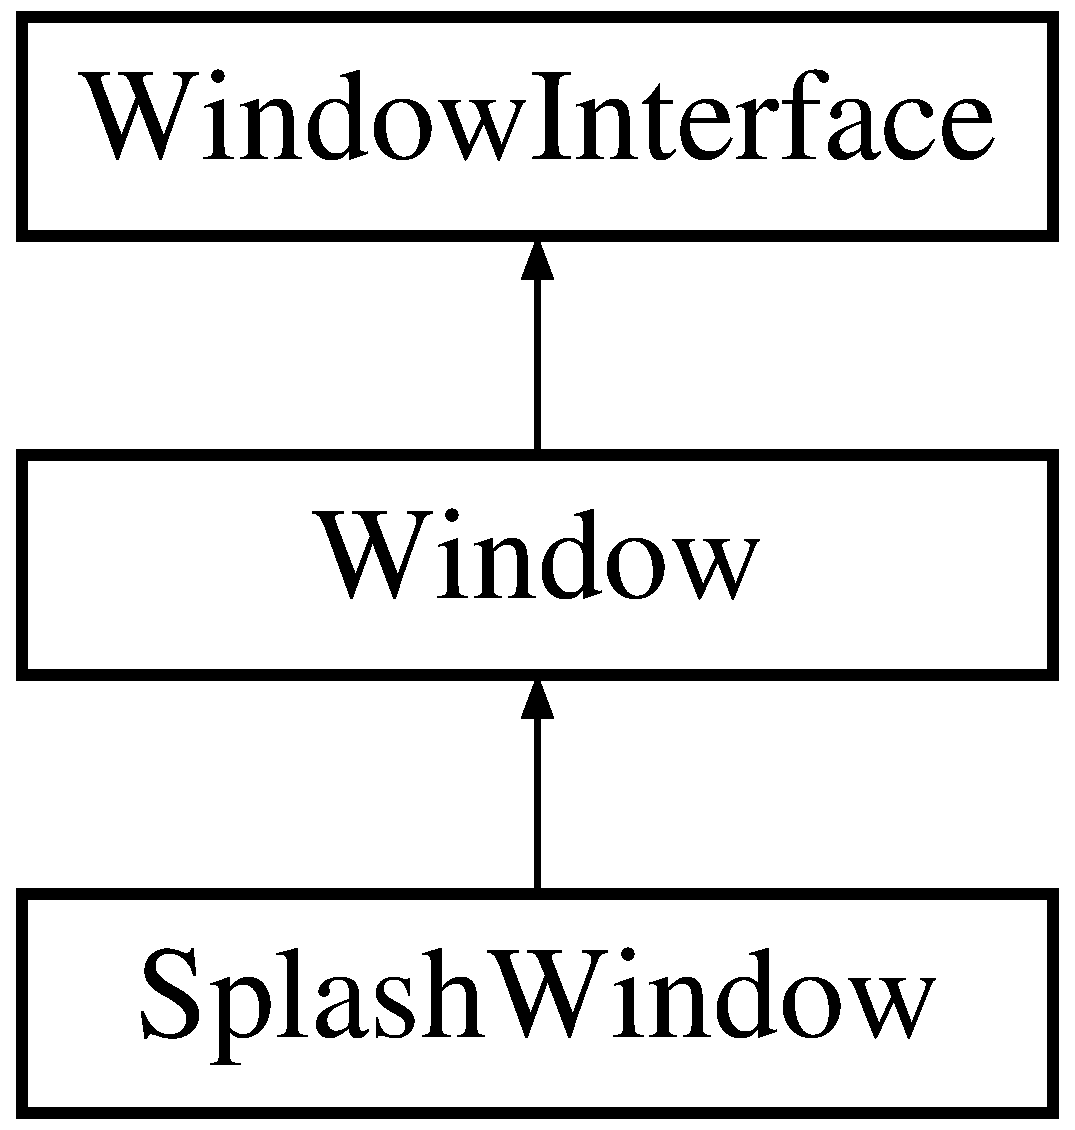
\includegraphics[height=3.000000cm]{classSplashWindow}
\end{center}
\end{figure}
\subsection*{Public Member Functions}
\begin{DoxyCompactItemize}
\item 
virtual void \hyperlink{classSplashWindow_aad27778951eb9dd5dbb03635f2bda114}{redraw} ()
\item 
virtual void \hyperlink{classWindow_a3dcd22169bd4d40f4b35eafdea31f6dd}{initialise} (\hyperlink{classGameEngineInterface}{Game\-Engine\-Interface} $\ast$a\-\_\-engine)
\item 
virtual void \hyperlink{classWindow_ae0ed7fd17df30f2d262cb684560e0469}{destroy} (void)
\item 
virtual \hyperlink{classGameEngineInterface}{Game\-Engine\-Interface} $\ast$ \hyperlink{classWindow_a55a6e31e36665bd3bcffcd844f5f0385}{get\-Engine} ()
\item 
virtual void \hyperlink{classWindow_a25a5308909ec422bebb480c803e1233c}{key\-Down} (unsigned char key)
\item 
virtual void \hyperlink{classWindow_a249f5a9513be00e59428a1df37502c63}{key\-Up} (unsigned char key)
\item 
virtual bool \hyperlink{classWindow_ac0927d0b89776959c4a95dd6737f841f}{get\-Key} (unsigned char key)
\item 
virtual void \hyperlink{classWindow_ace3bd5e6614510fce97263eccc35c0ab}{mouse\-Down} (int x, int y, int button)
\item 
virtual void \hyperlink{classWindow_a2e2c7592975405513a05a2da6a512b1c}{mouse\-Up} (int x, int y, int button)
\item 
virtual bool \hyperlink{classWindow_ab824bd52a5a055e468f7b2cc3d0b4f54}{get\-Mouse\-Button} (int button)
\item 
virtual void \hyperlink{classWindow_a1344118a395cb2fc48d4a2359372b074}{before\-Redraw} ()
\item 
virtual void \hyperlink{classWindow_a05b1d6673e37db442ecd80c54d10e6b7}{after\-Redraw} ()
\item 
virtual void \hyperlink{classWindow_a6e4274c73728009132b7e0dfad42a8de}{resize} (int width, int height)
\end{DoxyCompactItemize}
\subsection*{Static Public Attributes}
\begin{DoxyCompactItemize}
\item 
static const int \hyperlink{classWindow_a78a36ba2259fdd12ad2cf3346430fb35}{M\-A\-X\-\_\-\-B\-U\-T\-T\-O\-N\-S} = 5
\end{DoxyCompactItemize}


\subsection{Member Function Documentation}
\hypertarget{classWindow_a05b1d6673e37db442ecd80c54d10e6b7}{\index{Splash\-Window@{Splash\-Window}!after\-Redraw@{after\-Redraw}}
\index{after\-Redraw@{after\-Redraw}!SplashWindow@{Splash\-Window}}
\subsubsection[{after\-Redraw}]{\setlength{\rightskip}{0pt plus 5cm}void Window\-::after\-Redraw (
\begin{DoxyParamCaption}
{}
\end{DoxyParamCaption}
)\hspace{0.3cm}{\ttfamily [virtual]}, {\ttfamily [inherited]}}}\label{classWindow_a05b1d6673e37db442ecd80c54d10e6b7}


Implements \hyperlink{classWindowInterface_a37e350fc8f4a97333400c03e8544b2eb}{Window\-Interface}.

\hypertarget{classWindow_a1344118a395cb2fc48d4a2359372b074}{\index{Splash\-Window@{Splash\-Window}!before\-Redraw@{before\-Redraw}}
\index{before\-Redraw@{before\-Redraw}!SplashWindow@{Splash\-Window}}
\subsubsection[{before\-Redraw}]{\setlength{\rightskip}{0pt plus 5cm}void Window\-::before\-Redraw (
\begin{DoxyParamCaption}
{}
\end{DoxyParamCaption}
)\hspace{0.3cm}{\ttfamily [virtual]}, {\ttfamily [inherited]}}}\label{classWindow_a1344118a395cb2fc48d4a2359372b074}


Implements \hyperlink{classWindowInterface_a8aa6ce7a663628e3bd0480d4566191d2}{Window\-Interface}.

\hypertarget{classWindow_ae0ed7fd17df30f2d262cb684560e0469}{\index{Splash\-Window@{Splash\-Window}!destroy@{destroy}}
\index{destroy@{destroy}!SplashWindow@{Splash\-Window}}
\subsubsection[{destroy}]{\setlength{\rightskip}{0pt plus 5cm}void Window\-::destroy (
\begin{DoxyParamCaption}
\item[{void}]{}
\end{DoxyParamCaption}
)\hspace{0.3cm}{\ttfamily [virtual]}, {\ttfamily [inherited]}}}\label{classWindow_ae0ed7fd17df30f2d262cb684560e0469}


Implements \hyperlink{classWindowInterface_afeaed24b8e350acb196964106f2a0146}{Window\-Interface}.

\hypertarget{classWindow_a55a6e31e36665bd3bcffcd844f5f0385}{\index{Splash\-Window@{Splash\-Window}!get\-Engine@{get\-Engine}}
\index{get\-Engine@{get\-Engine}!SplashWindow@{Splash\-Window}}
\subsubsection[{get\-Engine}]{\setlength{\rightskip}{0pt plus 5cm}virtual {\bf Game\-Engine\-Interface}$\ast$ Window\-::get\-Engine (
\begin{DoxyParamCaption}
{}
\end{DoxyParamCaption}
)\hspace{0.3cm}{\ttfamily [inline]}, {\ttfamily [virtual]}, {\ttfamily [inherited]}}}\label{classWindow_a55a6e31e36665bd3bcffcd844f5f0385}


Implements \hyperlink{classWindowInterface_ac5970434199b518109a95a5cb645814a}{Window\-Interface}.

\hypertarget{classWindow_ac0927d0b89776959c4a95dd6737f841f}{\index{Splash\-Window@{Splash\-Window}!get\-Key@{get\-Key}}
\index{get\-Key@{get\-Key}!SplashWindow@{Splash\-Window}}
\subsubsection[{get\-Key}]{\setlength{\rightskip}{0pt plus 5cm}virtual bool Window\-::get\-Key (
\begin{DoxyParamCaption}
\item[{unsigned char}]{key}
\end{DoxyParamCaption}
)\hspace{0.3cm}{\ttfamily [inline]}, {\ttfamily [virtual]}, {\ttfamily [inherited]}}}\label{classWindow_ac0927d0b89776959c4a95dd6737f841f}


Implements \hyperlink{classWindowInterface_ab67d23a3dee052fd5901a87518b86e4d}{Window\-Interface}.

\hypertarget{classWindow_ab824bd52a5a055e468f7b2cc3d0b4f54}{\index{Splash\-Window@{Splash\-Window}!get\-Mouse\-Button@{get\-Mouse\-Button}}
\index{get\-Mouse\-Button@{get\-Mouse\-Button}!SplashWindow@{Splash\-Window}}
\subsubsection[{get\-Mouse\-Button}]{\setlength{\rightskip}{0pt plus 5cm}bool Window\-::get\-Mouse\-Button (
\begin{DoxyParamCaption}
\item[{int}]{button}
\end{DoxyParamCaption}
)\hspace{0.3cm}{\ttfamily [virtual]}, {\ttfamily [inherited]}}}\label{classWindow_ab824bd52a5a055e468f7b2cc3d0b4f54}
\hypertarget{classWindow_a3dcd22169bd4d40f4b35eafdea31f6dd}{\index{Splash\-Window@{Splash\-Window}!initialise@{initialise}}
\index{initialise@{initialise}!SplashWindow@{Splash\-Window}}
\subsubsection[{initialise}]{\setlength{\rightskip}{0pt plus 5cm}void Window\-::initialise (
\begin{DoxyParamCaption}
\item[{{\bf Game\-Engine\-Interface} $\ast$}]{a\-\_\-engine}
\end{DoxyParamCaption}
)\hspace{0.3cm}{\ttfamily [virtual]}, {\ttfamily [inherited]}}}\label{classWindow_a3dcd22169bd4d40f4b35eafdea31f6dd}


Implements \hyperlink{classWindowInterface_a8277c1eb7d3ae7b3f13e06081ffcf66a}{Window\-Interface}.



Reimplemented in \hyperlink{classMapWindow_affdeec7b3b899c38f16d04d170970e70}{Map\-Window}.

\hypertarget{classWindow_a25a5308909ec422bebb480c803e1233c}{\index{Splash\-Window@{Splash\-Window}!key\-Down@{key\-Down}}
\index{key\-Down@{key\-Down}!SplashWindow@{Splash\-Window}}
\subsubsection[{key\-Down}]{\setlength{\rightskip}{0pt plus 5cm}virtual void Window\-::key\-Down (
\begin{DoxyParamCaption}
\item[{unsigned char}]{key}
\end{DoxyParamCaption}
)\hspace{0.3cm}{\ttfamily [inline]}, {\ttfamily [virtual]}, {\ttfamily [inherited]}}}\label{classWindow_a25a5308909ec422bebb480c803e1233c}


Implements \hyperlink{classWindowInterface_a874548802028401146c44f7ba3e54d1d}{Window\-Interface}.



Reimplemented in \hyperlink{classMapWindow_a289795e503a5aa600e4091f5aa8b0b8c}{Map\-Window}.

\hypertarget{classWindow_a249f5a9513be00e59428a1df37502c63}{\index{Splash\-Window@{Splash\-Window}!key\-Up@{key\-Up}}
\index{key\-Up@{key\-Up}!SplashWindow@{Splash\-Window}}
\subsubsection[{key\-Up}]{\setlength{\rightskip}{0pt plus 5cm}virtual void Window\-::key\-Up (
\begin{DoxyParamCaption}
\item[{unsigned char}]{key}
\end{DoxyParamCaption}
)\hspace{0.3cm}{\ttfamily [inline]}, {\ttfamily [virtual]}, {\ttfamily [inherited]}}}\label{classWindow_a249f5a9513be00e59428a1df37502c63}


Implements \hyperlink{classWindowInterface_aa776c5cf4ef3d93a49613e08c79cab77}{Window\-Interface}.

\hypertarget{classWindow_ace3bd5e6614510fce97263eccc35c0ab}{\index{Splash\-Window@{Splash\-Window}!mouse\-Down@{mouse\-Down}}
\index{mouse\-Down@{mouse\-Down}!SplashWindow@{Splash\-Window}}
\subsubsection[{mouse\-Down}]{\setlength{\rightskip}{0pt plus 5cm}void Window\-::mouse\-Down (
\begin{DoxyParamCaption}
\item[{int}]{x, }
\item[{int}]{y, }
\item[{int}]{button}
\end{DoxyParamCaption}
)\hspace{0.3cm}{\ttfamily [virtual]}, {\ttfamily [inherited]}}}\label{classWindow_ace3bd5e6614510fce97263eccc35c0ab}


Implements \hyperlink{classWindowInterface_a5e6ba2b8e6560e9e3b74794cfd123d59}{Window\-Interface}.

\hypertarget{classWindow_a2e2c7592975405513a05a2da6a512b1c}{\index{Splash\-Window@{Splash\-Window}!mouse\-Up@{mouse\-Up}}
\index{mouse\-Up@{mouse\-Up}!SplashWindow@{Splash\-Window}}
\subsubsection[{mouse\-Up}]{\setlength{\rightskip}{0pt plus 5cm}void Window\-::mouse\-Up (
\begin{DoxyParamCaption}
\item[{int}]{x, }
\item[{int}]{y, }
\item[{int}]{button}
\end{DoxyParamCaption}
)\hspace{0.3cm}{\ttfamily [virtual]}, {\ttfamily [inherited]}}}\label{classWindow_a2e2c7592975405513a05a2da6a512b1c}


Implements \hyperlink{classWindowInterface_a482961a40e4a07d7f7ac81fe62ee7762}{Window\-Interface}.

\hypertarget{classSplashWindow_aad27778951eb9dd5dbb03635f2bda114}{\index{Splash\-Window@{Splash\-Window}!redraw@{redraw}}
\index{redraw@{redraw}!SplashWindow@{Splash\-Window}}
\subsubsection[{redraw}]{\setlength{\rightskip}{0pt plus 5cm}void Splash\-Window\-::redraw (
\begin{DoxyParamCaption}
{}
\end{DoxyParamCaption}
)\hspace{0.3cm}{\ttfamily [virtual]}}}\label{classSplashWindow_aad27778951eb9dd5dbb03635f2bda114}


Reimplemented from \hyperlink{classWindow_aa8b52b7035a78ef960c194c9bb4a7c36}{Window}.

\hypertarget{classWindow_a6e4274c73728009132b7e0dfad42a8de}{\index{Splash\-Window@{Splash\-Window}!resize@{resize}}
\index{resize@{resize}!SplashWindow@{Splash\-Window}}
\subsubsection[{resize}]{\setlength{\rightskip}{0pt plus 5cm}void Window\-::resize (
\begin{DoxyParamCaption}
\item[{int}]{width, }
\item[{int}]{height}
\end{DoxyParamCaption}
)\hspace{0.3cm}{\ttfamily [virtual]}, {\ttfamily [inherited]}}}\label{classWindow_a6e4274c73728009132b7e0dfad42a8de}


Implements \hyperlink{classWindowInterface_aa7109fc50fd3e90b0589bdd2a5e6972e}{Window\-Interface}.



\subsection{Member Data Documentation}
\hypertarget{classWindow_a78a36ba2259fdd12ad2cf3346430fb35}{\index{Splash\-Window@{Splash\-Window}!M\-A\-X\-\_\-\-B\-U\-T\-T\-O\-N\-S@{M\-A\-X\-\_\-\-B\-U\-T\-T\-O\-N\-S}}
\index{M\-A\-X\-\_\-\-B\-U\-T\-T\-O\-N\-S@{M\-A\-X\-\_\-\-B\-U\-T\-T\-O\-N\-S}!SplashWindow@{Splash\-Window}}
\subsubsection[{M\-A\-X\-\_\-\-B\-U\-T\-T\-O\-N\-S}]{\setlength{\rightskip}{0pt plus 5cm}const int Window\-::\-M\-A\-X\-\_\-\-B\-U\-T\-T\-O\-N\-S = 5\hspace{0.3cm}{\ttfamily [static]}, {\ttfamily [inherited]}}}\label{classWindow_a78a36ba2259fdd12ad2cf3346430fb35}


The documentation for this class was generated from the following files\-:\begin{DoxyCompactItemize}
\item 
\hyperlink{splash__window_8h}{splash\-\_\-window.\-h}\item 
\hyperlink{splash__window_8cpp}{splash\-\_\-window.\-cpp}\end{DoxyCompactItemize}

\hypertarget{structSpriteComponent}{\section{Sprite\-Component Struct Reference}
\label{structSpriteComponent}\index{Sprite\-Component@{Sprite\-Component}}
}


{\ttfamily \#include $<$sprite\-\_\-component.\-h$>$}

\subsection*{Public Attributes}
\begin{DoxyCompactItemize}
\item 
\hyperlink{classColor}{Color} \hyperlink{structSpriteComponent_a057de96f1a2de2f38e98c5fcdbb9cedc}{fg\-Color}
\item 
\hyperlink{classColor}{Color} \hyperlink{structSpriteComponent_a7343c020be982393fee296ea7c08bc0c}{bg\-Color}
\item 
unsigned int \hyperlink{structSpriteComponent_a27597e6299ef371db796928d6cdc54db}{sprite}
\item 
unsigned int \hyperlink{structSpriteComponent_af3b4dbdac3f132358f2dd983ec487a9e}{x\-Pos}
\item 
unsigned int \hyperlink{structSpriteComponent_aabf6f09bdbf8531b41ceb6f9bc20a773}{y\-Pos}
\end{DoxyCompactItemize}


\subsection{Member Data Documentation}
\hypertarget{structSpriteComponent_a7343c020be982393fee296ea7c08bc0c}{\index{Sprite\-Component@{Sprite\-Component}!bg\-Color@{bg\-Color}}
\index{bg\-Color@{bg\-Color}!SpriteComponent@{Sprite\-Component}}
\subsubsection[{bg\-Color}]{\setlength{\rightskip}{0pt plus 5cm}{\bf Color} Sprite\-Component\-::bg\-Color}}\label{structSpriteComponent_a7343c020be982393fee296ea7c08bc0c}
\hypertarget{structSpriteComponent_a057de96f1a2de2f38e98c5fcdbb9cedc}{\index{Sprite\-Component@{Sprite\-Component}!fg\-Color@{fg\-Color}}
\index{fg\-Color@{fg\-Color}!SpriteComponent@{Sprite\-Component}}
\subsubsection[{fg\-Color}]{\setlength{\rightskip}{0pt plus 5cm}{\bf Color} Sprite\-Component\-::fg\-Color}}\label{structSpriteComponent_a057de96f1a2de2f38e98c5fcdbb9cedc}
\hypertarget{structSpriteComponent_a27597e6299ef371db796928d6cdc54db}{\index{Sprite\-Component@{Sprite\-Component}!sprite@{sprite}}
\index{sprite@{sprite}!SpriteComponent@{Sprite\-Component}}
\subsubsection[{sprite}]{\setlength{\rightskip}{0pt plus 5cm}unsigned int Sprite\-Component\-::sprite}}\label{structSpriteComponent_a27597e6299ef371db796928d6cdc54db}
\hypertarget{structSpriteComponent_af3b4dbdac3f132358f2dd983ec487a9e}{\index{Sprite\-Component@{Sprite\-Component}!x\-Pos@{x\-Pos}}
\index{x\-Pos@{x\-Pos}!SpriteComponent@{Sprite\-Component}}
\subsubsection[{x\-Pos}]{\setlength{\rightskip}{0pt plus 5cm}unsigned int Sprite\-Component\-::x\-Pos}}\label{structSpriteComponent_af3b4dbdac3f132358f2dd983ec487a9e}
\hypertarget{structSpriteComponent_aabf6f09bdbf8531b41ceb6f9bc20a773}{\index{Sprite\-Component@{Sprite\-Component}!y\-Pos@{y\-Pos}}
\index{y\-Pos@{y\-Pos}!SpriteComponent@{Sprite\-Component}}
\subsubsection[{y\-Pos}]{\setlength{\rightskip}{0pt plus 5cm}unsigned int Sprite\-Component\-::y\-Pos}}\label{structSpriteComponent_aabf6f09bdbf8531b41ceb6f9bc20a773}


The documentation for this struct was generated from the following file\-:\begin{DoxyCompactItemize}
\item 
\hyperlink{sprite__component_8h}{sprite\-\_\-component.\-h}\end{DoxyCompactItemize}

\hypertarget{classSpriteSystem}{\section{Sprite\-System Class Reference}
\label{classSpriteSystem}\index{Sprite\-System@{Sprite\-System}}
}


{\ttfamily \#include $<$sprite\-\_\-system.\-h$>$}

Inheritance diagram for Sprite\-System\-:\begin{figure}[H]
\begin{center}
\leavevmode
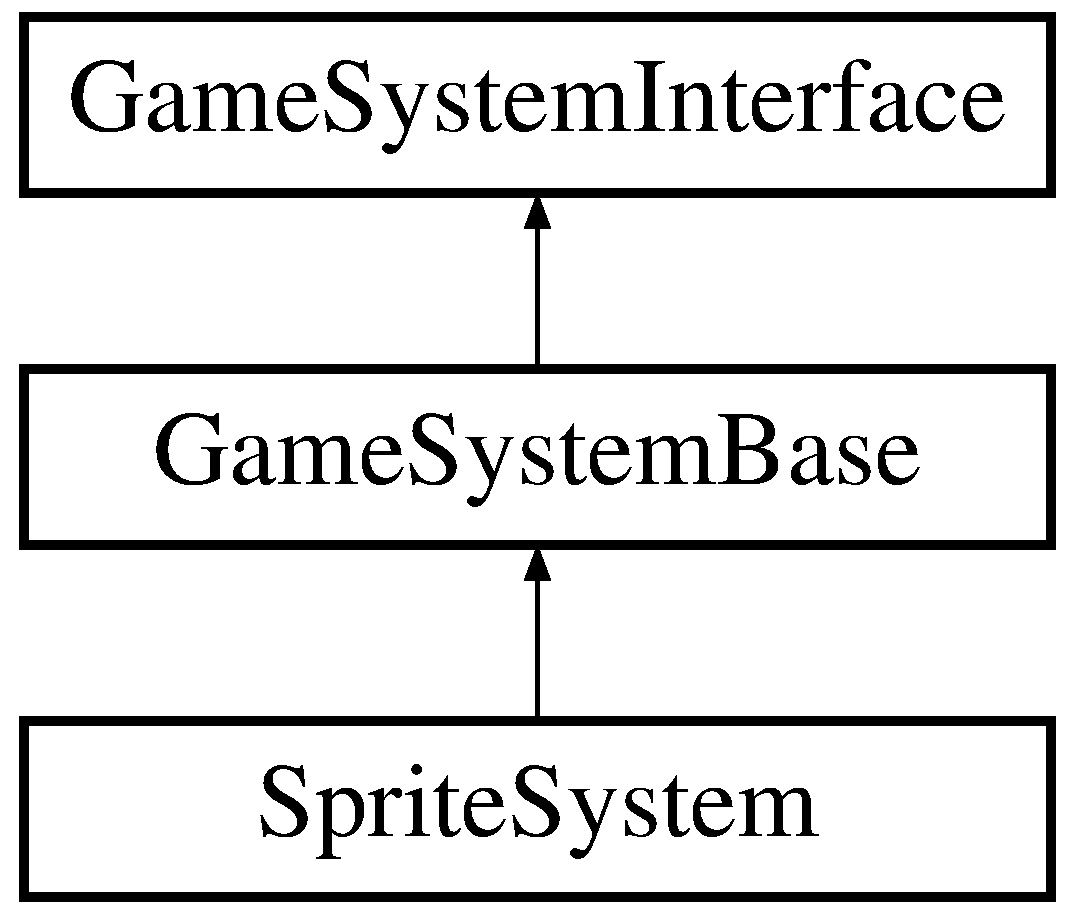
\includegraphics[height=3.000000cm]{classSpriteSystem}
\end{center}
\end{figure}
\subsection*{Public Member Functions}
\begin{DoxyCompactItemize}
\item 
virtual \hyperlink{classSpriteSystem_a7ce2844dbbc680db88085b72e583049a}{$\sim$\-Sprite\-System} ()
\item 
virtual void \hyperlink{classSpriteSystem_a52c4236903911045c117fd4771300faf}{handle\-Event} (const \hyperlink{classEvent}{Event} $\ast$event)
\item 
virtual void \hyperlink{classGameSystemBase_a55b4fc27cbfccd3c724c2e5984d78625}{initialise} (\hyperlink{classGameEngineInterface}{Game\-Engine\-Interface} $\ast$engine)
\item 
virtual \hyperlink{classGameEngineInterface}{Game\-Engine\-Interface} $\ast$ \hyperlink{classGameSystemBase_a1954c5a1c79963554805bc25b2cd6072}{get\-Engine\-Ref} ()
\item 
virtual void \hyperlink{classGameSystemBase_a039d3086ac7fe50abdb110b569520d69}{update} ()
\item 
virtual std\-::vector$<$ \hyperlink{classEntity}{Entity} $\ast$ $>$ \hyperlink{classGameSystemBase_aae270a88f1077a091e6033514b889abd}{find\-Entities\-Near} (unsigned int x, unsigned int y, unsigned radius)
\item 
virtual std\-::vector$<$ \hyperlink{classEntity}{Entity} $\ast$ $>$ \hyperlink{classGameSystemBase_a7aa9912fc078d990dbfb480e411bd3bc}{find\-Entities\-At} (unsigned int x, unsigned int y)
\item 
virtual std\-::vector$<$ \hyperlink{classEntity}{Entity} $\ast$ $>$ \hyperlink{classGameSystemBase_a44456ef40ac565b9d6b65f3b1531a4ef}{find\-Entities\-To\-The} (\hyperlink{classMoveEntityEvent_a7058a943643bee9164a21e62e3392807}{Move\-Entity\-Event\-::\-D\-I\-R\-E\-C\-T\-I\-O\-N} a\-\_\-direction, \hyperlink{classEntity}{Entity} $\ast$a\-\_\-entity)
\end{DoxyCompactItemize}
\subsection*{Protected Attributes}
\begin{DoxyCompactItemize}
\item 
\hyperlink{classGameEngineInterface}{Game\-Engine\-Interface} $\ast$ \hyperlink{classGameSystemBase_aa9044eb22399f0c0ddd8f049738c62e5}{m\-\_\-engine}
\end{DoxyCompactItemize}
\subsection*{Private Member Functions}
\begin{DoxyCompactItemize}
\item 
void \hyperlink{classSpriteSystem_a74dfa4e4d371d3d8722e96f7c6ac399c}{handle\-Add\-Wall\-Event} (\hyperlink{classEntity}{Entity} $\ast$a\-\_\-entity)
\item 
\hyperlink{classEntity}{Entity} $\ast$ \hyperlink{classSpriteSystem_ae12fa3467ee8fdb5dc5cd85ba8181770}{find\-Wall\-Entity} (unsigned int x, unsigned int y)
\item 
void \hyperlink{classSpriteSystem_a76ccc3de7d715fe015a10c5fdb4b1d39}{update\-Wall\-Sprite} (\hyperlink{classEntity}{Entity} $\ast$a\-\_\-entity)
\end{DoxyCompactItemize}


\subsection{Constructor \& Destructor Documentation}
\hypertarget{classSpriteSystem_a7ce2844dbbc680db88085b72e583049a}{\index{Sprite\-System@{Sprite\-System}!$\sim$\-Sprite\-System@{$\sim$\-Sprite\-System}}
\index{$\sim$\-Sprite\-System@{$\sim$\-Sprite\-System}!SpriteSystem@{Sprite\-System}}
\subsubsection[{$\sim$\-Sprite\-System}]{\setlength{\rightskip}{0pt plus 5cm}virtual Sprite\-System\-::$\sim$\-Sprite\-System (
\begin{DoxyParamCaption}
{}
\end{DoxyParamCaption}
)\hspace{0.3cm}{\ttfamily [inline]}, {\ttfamily [virtual]}}}\label{classSpriteSystem_a7ce2844dbbc680db88085b72e583049a}


\subsection{Member Function Documentation}
\hypertarget{classGameSystemBase_a7aa9912fc078d990dbfb480e411bd3bc}{\index{Sprite\-System@{Sprite\-System}!find\-Entities\-At@{find\-Entities\-At}}
\index{find\-Entities\-At@{find\-Entities\-At}!SpriteSystem@{Sprite\-System}}
\subsubsection[{find\-Entities\-At}]{\setlength{\rightskip}{0pt plus 5cm}std\-::vector$<$ {\bf Entity} $\ast$ $>$ Game\-System\-Base\-::find\-Entities\-At (
\begin{DoxyParamCaption}
\item[{unsigned int}]{x, }
\item[{unsigned int}]{y}
\end{DoxyParamCaption}
)\hspace{0.3cm}{\ttfamily [virtual]}, {\ttfamily [inherited]}}}\label{classGameSystemBase_a7aa9912fc078d990dbfb480e411bd3bc}
\hypertarget{classGameSystemBase_aae270a88f1077a091e6033514b889abd}{\index{Sprite\-System@{Sprite\-System}!find\-Entities\-Near@{find\-Entities\-Near}}
\index{find\-Entities\-Near@{find\-Entities\-Near}!SpriteSystem@{Sprite\-System}}
\subsubsection[{find\-Entities\-Near}]{\setlength{\rightskip}{0pt plus 5cm}std\-::vector$<$ {\bf Entity} $\ast$ $>$ Game\-System\-Base\-::find\-Entities\-Near (
\begin{DoxyParamCaption}
\item[{unsigned int}]{x, }
\item[{unsigned int}]{y, }
\item[{unsigned}]{radius}
\end{DoxyParamCaption}
)\hspace{0.3cm}{\ttfamily [virtual]}, {\ttfamily [inherited]}}}\label{classGameSystemBase_aae270a88f1077a091e6033514b889abd}
\hypertarget{classGameSystemBase_a44456ef40ac565b9d6b65f3b1531a4ef}{\index{Sprite\-System@{Sprite\-System}!find\-Entities\-To\-The@{find\-Entities\-To\-The}}
\index{find\-Entities\-To\-The@{find\-Entities\-To\-The}!SpriteSystem@{Sprite\-System}}
\subsubsection[{find\-Entities\-To\-The}]{\setlength{\rightskip}{0pt plus 5cm}std\-::vector$<$ {\bf Entity} $\ast$ $>$ Game\-System\-Base\-::find\-Entities\-To\-The (
\begin{DoxyParamCaption}
\item[{{\bf Move\-Entity\-Event\-::\-D\-I\-R\-E\-C\-T\-I\-O\-N}}]{a\-\_\-direction, }
\item[{{\bf Entity} $\ast$}]{a\-\_\-entity}
\end{DoxyParamCaption}
)\hspace{0.3cm}{\ttfamily [virtual]}, {\ttfamily [inherited]}}}\label{classGameSystemBase_a44456ef40ac565b9d6b65f3b1531a4ef}
\hypertarget{classSpriteSystem_ae12fa3467ee8fdb5dc5cd85ba8181770}{\index{Sprite\-System@{Sprite\-System}!find\-Wall\-Entity@{find\-Wall\-Entity}}
\index{find\-Wall\-Entity@{find\-Wall\-Entity}!SpriteSystem@{Sprite\-System}}
\subsubsection[{find\-Wall\-Entity}]{\setlength{\rightskip}{0pt plus 5cm}{\bf Entity} $\ast$ Sprite\-System\-::find\-Wall\-Entity (
\begin{DoxyParamCaption}
\item[{unsigned int}]{x, }
\item[{unsigned int}]{y}
\end{DoxyParamCaption}
)\hspace{0.3cm}{\ttfamily [private]}}}\label{classSpriteSystem_ae12fa3467ee8fdb5dc5cd85ba8181770}
\hypertarget{classGameSystemBase_a1954c5a1c79963554805bc25b2cd6072}{\index{Sprite\-System@{Sprite\-System}!get\-Engine\-Ref@{get\-Engine\-Ref}}
\index{get\-Engine\-Ref@{get\-Engine\-Ref}!SpriteSystem@{Sprite\-System}}
\subsubsection[{get\-Engine\-Ref}]{\setlength{\rightskip}{0pt plus 5cm}virtual {\bf Game\-Engine\-Interface}$\ast$ Game\-System\-Base\-::get\-Engine\-Ref (
\begin{DoxyParamCaption}
{}
\end{DoxyParamCaption}
)\hspace{0.3cm}{\ttfamily [inline]}, {\ttfamily [virtual]}, {\ttfamily [inherited]}}}\label{classGameSystemBase_a1954c5a1c79963554805bc25b2cd6072}
\hypertarget{classSpriteSystem_a74dfa4e4d371d3d8722e96f7c6ac399c}{\index{Sprite\-System@{Sprite\-System}!handle\-Add\-Wall\-Event@{handle\-Add\-Wall\-Event}}
\index{handle\-Add\-Wall\-Event@{handle\-Add\-Wall\-Event}!SpriteSystem@{Sprite\-System}}
\subsubsection[{handle\-Add\-Wall\-Event}]{\setlength{\rightskip}{0pt plus 5cm}void Sprite\-System\-::handle\-Add\-Wall\-Event (
\begin{DoxyParamCaption}
\item[{{\bf Entity} $\ast$}]{a\-\_\-entity}
\end{DoxyParamCaption}
)\hspace{0.3cm}{\ttfamily [private]}}}\label{classSpriteSystem_a74dfa4e4d371d3d8722e96f7c6ac399c}
\hypertarget{classSpriteSystem_a52c4236903911045c117fd4771300faf}{\index{Sprite\-System@{Sprite\-System}!handle\-Event@{handle\-Event}}
\index{handle\-Event@{handle\-Event}!SpriteSystem@{Sprite\-System}}
\subsubsection[{handle\-Event}]{\setlength{\rightskip}{0pt plus 5cm}void Sprite\-System\-::handle\-Event (
\begin{DoxyParamCaption}
\item[{const {\bf Event} $\ast$}]{event}
\end{DoxyParamCaption}
)\hspace{0.3cm}{\ttfamily [virtual]}}}\label{classSpriteSystem_a52c4236903911045c117fd4771300faf}


Reimplemented from \hyperlink{classGameSystemBase_a007b3ece290b1ad0dc3e397c5264d44d}{Game\-System\-Base}.

\hypertarget{classGameSystemBase_a55b4fc27cbfccd3c724c2e5984d78625}{\index{Sprite\-System@{Sprite\-System}!initialise@{initialise}}
\index{initialise@{initialise}!SpriteSystem@{Sprite\-System}}
\subsubsection[{initialise}]{\setlength{\rightskip}{0pt plus 5cm}virtual void Game\-System\-Base\-::initialise (
\begin{DoxyParamCaption}
\item[{{\bf Game\-Engine\-Interface} $\ast$}]{engine}
\end{DoxyParamCaption}
)\hspace{0.3cm}{\ttfamily [inline]}, {\ttfamily [virtual]}, {\ttfamily [inherited]}}}\label{classGameSystemBase_a55b4fc27cbfccd3c724c2e5984d78625}


Implements \hyperlink{classGameSystemInterface_a29079ef1f35027150b751c3fcb025091}{Game\-System\-Interface}.

\hypertarget{classGameSystemBase_a039d3086ac7fe50abdb110b569520d69}{\index{Sprite\-System@{Sprite\-System}!update@{update}}
\index{update@{update}!SpriteSystem@{Sprite\-System}}
\subsubsection[{update}]{\setlength{\rightskip}{0pt plus 5cm}virtual void Game\-System\-Base\-::update (
\begin{DoxyParamCaption}
{}
\end{DoxyParamCaption}
)\hspace{0.3cm}{\ttfamily [inline]}, {\ttfamily [virtual]}, {\ttfamily [inherited]}}}\label{classGameSystemBase_a039d3086ac7fe50abdb110b569520d69}


Implements \hyperlink{classGameSystemInterface_a531f5e7c6ca9881a67932cc4fded0a2e}{Game\-System\-Interface}.



Reimplemented in \hyperlink{classNpcSystem_a88d87a8ec981e5cf1f4ed4340123a9d8}{Npc\-System}.

\hypertarget{classSpriteSystem_a76ccc3de7d715fe015a10c5fdb4b1d39}{\index{Sprite\-System@{Sprite\-System}!update\-Wall\-Sprite@{update\-Wall\-Sprite}}
\index{update\-Wall\-Sprite@{update\-Wall\-Sprite}!SpriteSystem@{Sprite\-System}}
\subsubsection[{update\-Wall\-Sprite}]{\setlength{\rightskip}{0pt plus 5cm}void Sprite\-System\-::update\-Wall\-Sprite (
\begin{DoxyParamCaption}
\item[{{\bf Entity} $\ast$}]{a\-\_\-entity}
\end{DoxyParamCaption}
)\hspace{0.3cm}{\ttfamily [private]}}}\label{classSpriteSystem_a76ccc3de7d715fe015a10c5fdb4b1d39}


\subsection{Member Data Documentation}
\hypertarget{classGameSystemBase_aa9044eb22399f0c0ddd8f049738c62e5}{\index{Sprite\-System@{Sprite\-System}!m\-\_\-engine@{m\-\_\-engine}}
\index{m\-\_\-engine@{m\-\_\-engine}!SpriteSystem@{Sprite\-System}}
\subsubsection[{m\-\_\-engine}]{\setlength{\rightskip}{0pt plus 5cm}{\bf Game\-Engine\-Interface}$\ast$ Game\-System\-Base\-::m\-\_\-engine\hspace{0.3cm}{\ttfamily [protected]}, {\ttfamily [inherited]}}}\label{classGameSystemBase_aa9044eb22399f0c0ddd8f049738c62e5}


The documentation for this class was generated from the following files\-:\begin{DoxyCompactItemize}
\item 
\hyperlink{sprite__system_8h}{sprite\-\_\-system.\-h}\item 
\hyperlink{sprite__system_8cpp}{sprite\-\_\-system.\-cpp}\end{DoxyCompactItemize}

\hypertarget{structTagValue}{\section{Tag\-Value Struct Reference}
\label{structTagValue}\index{Tag\-Value@{Tag\-Value}}
}


{\ttfamily \#include $<$config\-\_\-manager.\-h$>$}

\subsection*{Public Attributes}
\begin{DoxyCompactItemize}
\item 
std\-::string \hyperlink{structTagValue_ad588e4c422bcef3e428b1e7a53018e9b}{str}
\item 
long \hyperlink{structTagValue_a968ed84fa6cfccba6ef104f663ae3c08}{num}
\item 
double \hyperlink{structTagValue_a641f80e1d15c3c3e60e1cec4a83c952b}{dec}
\end{DoxyCompactItemize}


\subsection{Member Data Documentation}
\hypertarget{structTagValue_a641f80e1d15c3c3e60e1cec4a83c952b}{\index{Tag\-Value@{Tag\-Value}!dec@{dec}}
\index{dec@{dec}!TagValue@{Tag\-Value}}
\subsubsection[{dec}]{\setlength{\rightskip}{0pt plus 5cm}double Tag\-Value\-::dec}}\label{structTagValue_a641f80e1d15c3c3e60e1cec4a83c952b}
\hypertarget{structTagValue_a968ed84fa6cfccba6ef104f663ae3c08}{\index{Tag\-Value@{Tag\-Value}!num@{num}}
\index{num@{num}!TagValue@{Tag\-Value}}
\subsubsection[{num}]{\setlength{\rightskip}{0pt plus 5cm}long Tag\-Value\-::num}}\label{structTagValue_a968ed84fa6cfccba6ef104f663ae3c08}
\hypertarget{structTagValue_ad588e4c422bcef3e428b1e7a53018e9b}{\index{Tag\-Value@{Tag\-Value}!str@{str}}
\index{str@{str}!TagValue@{Tag\-Value}}
\subsubsection[{str}]{\setlength{\rightskip}{0pt plus 5cm}std\-::string Tag\-Value\-::str}}\label{structTagValue_ad588e4c422bcef3e428b1e7a53018e9b}


The documentation for this struct was generated from the following file\-:\begin{DoxyCompactItemize}
\item 
\hyperlink{config__manager_8h}{config\-\_\-manager.\-h}\end{DoxyCompactItemize}

\hypertarget{classWindow}{\section{Window Class Reference}
\label{classWindow}\index{Window@{Window}}
}


{\ttfamily \#include $<$window.\-h$>$}

Inheritance diagram for Window\-:\begin{figure}[H]
\begin{center}
\leavevmode
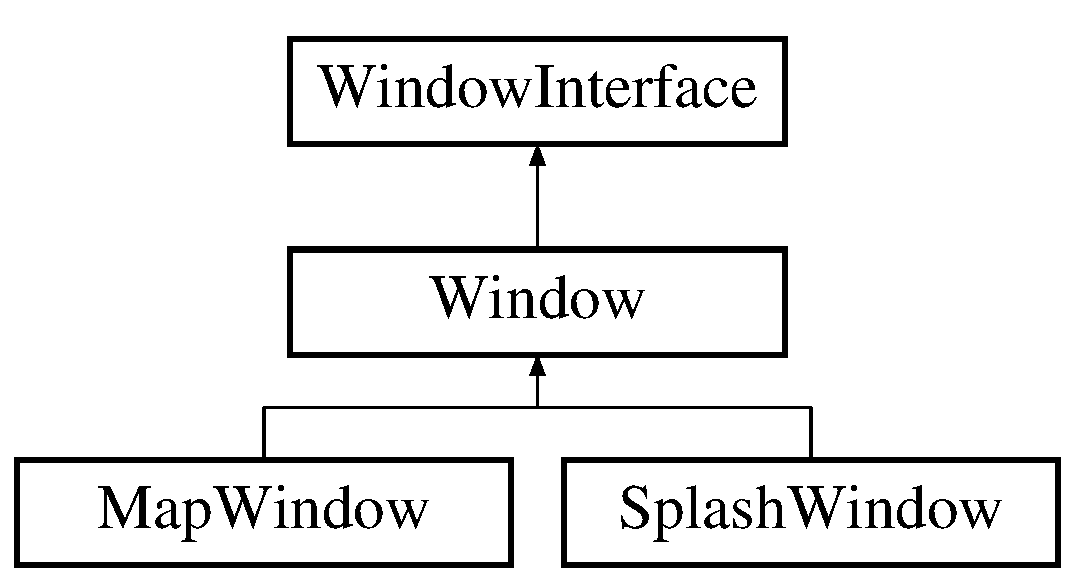
\includegraphics[height=3.000000cm]{classWindow}
\end{center}
\end{figure}
\subsection*{Public Member Functions}
\begin{DoxyCompactItemize}
\item 
\hyperlink{classWindow_a74e6087da23d3c24e9fac0245e5ec92c}{Window} ()
\item 
virtual \hyperlink{classWindow_a62b4a97b3c2e492f1d9a46092011e2d9}{$\sim$\-Window} ()
\item 
virtual void \hyperlink{classWindow_a3dcd22169bd4d40f4b35eafdea31f6dd}{initialise} (\hyperlink{classGameEngineInterface}{Game\-Engine\-Interface} $\ast$a\-\_\-engine)
\item 
virtual void \hyperlink{classWindow_ae0ed7fd17df30f2d262cb684560e0469}{destroy} (void)
\item 
virtual \hyperlink{classGameEngineInterface}{Game\-Engine\-Interface} $\ast$ \hyperlink{classWindow_a55a6e31e36665bd3bcffcd844f5f0385}{get\-Engine} ()
\item 
virtual void \hyperlink{classWindow_a25a5308909ec422bebb480c803e1233c}{key\-Down} (unsigned char key)
\item 
virtual void \hyperlink{classWindow_a249f5a9513be00e59428a1df37502c63}{key\-Up} (unsigned char key)
\item 
virtual bool \hyperlink{classWindow_ac0927d0b89776959c4a95dd6737f841f}{get\-Key} (unsigned char key)
\item 
virtual void \hyperlink{classWindow_ace3bd5e6614510fce97263eccc35c0ab}{mouse\-Down} (int x, int y, int button)
\item 
virtual void \hyperlink{classWindow_a2e2c7592975405513a05a2da6a512b1c}{mouse\-Up} (int x, int y, int button)
\item 
virtual bool \hyperlink{classWindow_ab824bd52a5a055e468f7b2cc3d0b4f54}{get\-Mouse\-Button} (int button)
\item 
virtual void \hyperlink{classWindow_a1344118a395cb2fc48d4a2359372b074}{before\-Redraw} ()
\item 
virtual void \hyperlink{classWindow_aa8b52b7035a78ef960c194c9bb4a7c36}{redraw} ()
\item 
virtual void \hyperlink{classWindow_a05b1d6673e37db442ecd80c54d10e6b7}{after\-Redraw} ()
\item 
virtual void \hyperlink{classWindow_a6e4274c73728009132b7e0dfad42a8de}{resize} (int width, int height)
\end{DoxyCompactItemize}
\subsection*{Static Public Attributes}
\begin{DoxyCompactItemize}
\item 
static const int \hyperlink{classWindow_a78a36ba2259fdd12ad2cf3346430fb35}{M\-A\-X\-\_\-\-B\-U\-T\-T\-O\-N\-S} = 5
\end{DoxyCompactItemize}
\subsection*{Private Attributes}
\begin{DoxyCompactItemize}
\item 
bool \hyperlink{classWindow_a821f2d3494f4f8942eb9785a11cb53a3}{ascii\-\_\-keys} \mbox{[}256\mbox{]}
\item 
bool \hyperlink{classWindow_aa0423e0229d8bfadfdb48dfc353a1f14}{special\-\_\-keys} \mbox{[}256\mbox{]}
\item 
int \hyperlink{classWindow_adf12eb74f1a9eb60cf9dd9e95ad73e07}{m\-\_\-buttons} \mbox{[}\hyperlink{classWindow_a78a36ba2259fdd12ad2cf3346430fb35}{M\-A\-X\-\_\-\-B\-U\-T\-T\-O\-N\-S}\mbox{]}
\item 
\hyperlink{classGameEngineInterface}{Game\-Engine\-Interface} $\ast$ \hyperlink{classWindow_ac9461ed7e87d19ee881a582909f7229b}{m\-\_\-engine}
\end{DoxyCompactItemize}


\subsection{Constructor \& Destructor Documentation}
\hypertarget{classWindow_a74e6087da23d3c24e9fac0245e5ec92c}{\index{Window@{Window}!Window@{Window}}
\index{Window@{Window}!Window@{Window}}
\subsubsection[{Window}]{\setlength{\rightskip}{0pt plus 5cm}Window\-::\-Window (
\begin{DoxyParamCaption}
{}
\end{DoxyParamCaption}
)\hspace{0.3cm}{\ttfamily [inline]}}}\label{classWindow_a74e6087da23d3c24e9fac0245e5ec92c}
\hypertarget{classWindow_a62b4a97b3c2e492f1d9a46092011e2d9}{\index{Window@{Window}!$\sim$\-Window@{$\sim$\-Window}}
\index{$\sim$\-Window@{$\sim$\-Window}!Window@{Window}}
\subsubsection[{$\sim$\-Window}]{\setlength{\rightskip}{0pt plus 5cm}virtual Window\-::$\sim$\-Window (
\begin{DoxyParamCaption}
{}
\end{DoxyParamCaption}
)\hspace{0.3cm}{\ttfamily [inline]}, {\ttfamily [virtual]}}}\label{classWindow_a62b4a97b3c2e492f1d9a46092011e2d9}


\subsection{Member Function Documentation}
\hypertarget{classWindow_a05b1d6673e37db442ecd80c54d10e6b7}{\index{Window@{Window}!after\-Redraw@{after\-Redraw}}
\index{after\-Redraw@{after\-Redraw}!Window@{Window}}
\subsubsection[{after\-Redraw}]{\setlength{\rightskip}{0pt plus 5cm}void Window\-::after\-Redraw (
\begin{DoxyParamCaption}
{}
\end{DoxyParamCaption}
)\hspace{0.3cm}{\ttfamily [virtual]}}}\label{classWindow_a05b1d6673e37db442ecd80c54d10e6b7}


Implements \hyperlink{classWindowInterface_a37e350fc8f4a97333400c03e8544b2eb}{Window\-Interface}.

\hypertarget{classWindow_a1344118a395cb2fc48d4a2359372b074}{\index{Window@{Window}!before\-Redraw@{before\-Redraw}}
\index{before\-Redraw@{before\-Redraw}!Window@{Window}}
\subsubsection[{before\-Redraw}]{\setlength{\rightskip}{0pt plus 5cm}void Window\-::before\-Redraw (
\begin{DoxyParamCaption}
{}
\end{DoxyParamCaption}
)\hspace{0.3cm}{\ttfamily [virtual]}}}\label{classWindow_a1344118a395cb2fc48d4a2359372b074}


Implements \hyperlink{classWindowInterface_a8aa6ce7a663628e3bd0480d4566191d2}{Window\-Interface}.

\hypertarget{classWindow_ae0ed7fd17df30f2d262cb684560e0469}{\index{Window@{Window}!destroy@{destroy}}
\index{destroy@{destroy}!Window@{Window}}
\subsubsection[{destroy}]{\setlength{\rightskip}{0pt plus 5cm}void Window\-::destroy (
\begin{DoxyParamCaption}
\item[{void}]{}
\end{DoxyParamCaption}
)\hspace{0.3cm}{\ttfamily [virtual]}}}\label{classWindow_ae0ed7fd17df30f2d262cb684560e0469}


Implements \hyperlink{classWindowInterface_afeaed24b8e350acb196964106f2a0146}{Window\-Interface}.

\hypertarget{classWindow_a55a6e31e36665bd3bcffcd844f5f0385}{\index{Window@{Window}!get\-Engine@{get\-Engine}}
\index{get\-Engine@{get\-Engine}!Window@{Window}}
\subsubsection[{get\-Engine}]{\setlength{\rightskip}{0pt plus 5cm}virtual {\bf Game\-Engine\-Interface}$\ast$ Window\-::get\-Engine (
\begin{DoxyParamCaption}
{}
\end{DoxyParamCaption}
)\hspace{0.3cm}{\ttfamily [inline]}, {\ttfamily [virtual]}}}\label{classWindow_a55a6e31e36665bd3bcffcd844f5f0385}


Implements \hyperlink{classWindowInterface_ac5970434199b518109a95a5cb645814a}{Window\-Interface}.

\hypertarget{classWindow_ac0927d0b89776959c4a95dd6737f841f}{\index{Window@{Window}!get\-Key@{get\-Key}}
\index{get\-Key@{get\-Key}!Window@{Window}}
\subsubsection[{get\-Key}]{\setlength{\rightskip}{0pt plus 5cm}virtual bool Window\-::get\-Key (
\begin{DoxyParamCaption}
\item[{unsigned char}]{key}
\end{DoxyParamCaption}
)\hspace{0.3cm}{\ttfamily [inline]}, {\ttfamily [virtual]}}}\label{classWindow_ac0927d0b89776959c4a95dd6737f841f}


Implements \hyperlink{classWindowInterface_ab67d23a3dee052fd5901a87518b86e4d}{Window\-Interface}.

\hypertarget{classWindow_ab824bd52a5a055e468f7b2cc3d0b4f54}{\index{Window@{Window}!get\-Mouse\-Button@{get\-Mouse\-Button}}
\index{get\-Mouse\-Button@{get\-Mouse\-Button}!Window@{Window}}
\subsubsection[{get\-Mouse\-Button}]{\setlength{\rightskip}{0pt plus 5cm}bool Window\-::get\-Mouse\-Button (
\begin{DoxyParamCaption}
\item[{int}]{button}
\end{DoxyParamCaption}
)\hspace{0.3cm}{\ttfamily [virtual]}}}\label{classWindow_ab824bd52a5a055e468f7b2cc3d0b4f54}
\hypertarget{classWindow_a3dcd22169bd4d40f4b35eafdea31f6dd}{\index{Window@{Window}!initialise@{initialise}}
\index{initialise@{initialise}!Window@{Window}}
\subsubsection[{initialise}]{\setlength{\rightskip}{0pt plus 5cm}void Window\-::initialise (
\begin{DoxyParamCaption}
\item[{{\bf Game\-Engine\-Interface} $\ast$}]{a\-\_\-engine}
\end{DoxyParamCaption}
)\hspace{0.3cm}{\ttfamily [virtual]}}}\label{classWindow_a3dcd22169bd4d40f4b35eafdea31f6dd}


Implements \hyperlink{classWindowInterface_a8277c1eb7d3ae7b3f13e06081ffcf66a}{Window\-Interface}.



Reimplemented in \hyperlink{classMapWindow_affdeec7b3b899c38f16d04d170970e70}{Map\-Window}.

\hypertarget{classWindow_a25a5308909ec422bebb480c803e1233c}{\index{Window@{Window}!key\-Down@{key\-Down}}
\index{key\-Down@{key\-Down}!Window@{Window}}
\subsubsection[{key\-Down}]{\setlength{\rightskip}{0pt plus 5cm}virtual void Window\-::key\-Down (
\begin{DoxyParamCaption}
\item[{unsigned char}]{key}
\end{DoxyParamCaption}
)\hspace{0.3cm}{\ttfamily [inline]}, {\ttfamily [virtual]}}}\label{classWindow_a25a5308909ec422bebb480c803e1233c}


Implements \hyperlink{classWindowInterface_a874548802028401146c44f7ba3e54d1d}{Window\-Interface}.



Reimplemented in \hyperlink{classMapWindow_a289795e503a5aa600e4091f5aa8b0b8c}{Map\-Window}.

\hypertarget{classWindow_a249f5a9513be00e59428a1df37502c63}{\index{Window@{Window}!key\-Up@{key\-Up}}
\index{key\-Up@{key\-Up}!Window@{Window}}
\subsubsection[{key\-Up}]{\setlength{\rightskip}{0pt plus 5cm}virtual void Window\-::key\-Up (
\begin{DoxyParamCaption}
\item[{unsigned char}]{key}
\end{DoxyParamCaption}
)\hspace{0.3cm}{\ttfamily [inline]}, {\ttfamily [virtual]}}}\label{classWindow_a249f5a9513be00e59428a1df37502c63}


Implements \hyperlink{classWindowInterface_aa776c5cf4ef3d93a49613e08c79cab77}{Window\-Interface}.

\hypertarget{classWindow_ace3bd5e6614510fce97263eccc35c0ab}{\index{Window@{Window}!mouse\-Down@{mouse\-Down}}
\index{mouse\-Down@{mouse\-Down}!Window@{Window}}
\subsubsection[{mouse\-Down}]{\setlength{\rightskip}{0pt plus 5cm}void Window\-::mouse\-Down (
\begin{DoxyParamCaption}
\item[{int}]{x, }
\item[{int}]{y, }
\item[{int}]{button}
\end{DoxyParamCaption}
)\hspace{0.3cm}{\ttfamily [virtual]}}}\label{classWindow_ace3bd5e6614510fce97263eccc35c0ab}


Implements \hyperlink{classWindowInterface_a5e6ba2b8e6560e9e3b74794cfd123d59}{Window\-Interface}.

\hypertarget{classWindow_a2e2c7592975405513a05a2da6a512b1c}{\index{Window@{Window}!mouse\-Up@{mouse\-Up}}
\index{mouse\-Up@{mouse\-Up}!Window@{Window}}
\subsubsection[{mouse\-Up}]{\setlength{\rightskip}{0pt plus 5cm}void Window\-::mouse\-Up (
\begin{DoxyParamCaption}
\item[{int}]{x, }
\item[{int}]{y, }
\item[{int}]{button}
\end{DoxyParamCaption}
)\hspace{0.3cm}{\ttfamily [virtual]}}}\label{classWindow_a2e2c7592975405513a05a2da6a512b1c}


Implements \hyperlink{classWindowInterface_a482961a40e4a07d7f7ac81fe62ee7762}{Window\-Interface}.

\hypertarget{classWindow_aa8b52b7035a78ef960c194c9bb4a7c36}{\index{Window@{Window}!redraw@{redraw}}
\index{redraw@{redraw}!Window@{Window}}
\subsubsection[{redraw}]{\setlength{\rightskip}{0pt plus 5cm}virtual void Window\-::redraw (
\begin{DoxyParamCaption}
{}
\end{DoxyParamCaption}
)\hspace{0.3cm}{\ttfamily [inline]}, {\ttfamily [virtual]}}}\label{classWindow_aa8b52b7035a78ef960c194c9bb4a7c36}


Implements \hyperlink{classWindowInterface_a9baf4b0e9c1fdd73b1fe14af4173c699}{Window\-Interface}.



Reimplemented in \hyperlink{classMapWindow_a5759338c3758b2a3252ffc691958dff8}{Map\-Window}, and \hyperlink{classSplashWindow_aad27778951eb9dd5dbb03635f2bda114}{Splash\-Window}.

\hypertarget{classWindow_a6e4274c73728009132b7e0dfad42a8de}{\index{Window@{Window}!resize@{resize}}
\index{resize@{resize}!Window@{Window}}
\subsubsection[{resize}]{\setlength{\rightskip}{0pt plus 5cm}void Window\-::resize (
\begin{DoxyParamCaption}
\item[{int}]{width, }
\item[{int}]{height}
\end{DoxyParamCaption}
)\hspace{0.3cm}{\ttfamily [virtual]}}}\label{classWindow_a6e4274c73728009132b7e0dfad42a8de}


Implements \hyperlink{classWindowInterface_aa7109fc50fd3e90b0589bdd2a5e6972e}{Window\-Interface}.



\subsection{Member Data Documentation}
\hypertarget{classWindow_a821f2d3494f4f8942eb9785a11cb53a3}{\index{Window@{Window}!ascii\-\_\-keys@{ascii\-\_\-keys}}
\index{ascii\-\_\-keys@{ascii\-\_\-keys}!Window@{Window}}
\subsubsection[{ascii\-\_\-keys}]{\setlength{\rightskip}{0pt plus 5cm}bool Window\-::ascii\-\_\-keys\mbox{[}256\mbox{]}\hspace{0.3cm}{\ttfamily [private]}}}\label{classWindow_a821f2d3494f4f8942eb9785a11cb53a3}
\hypertarget{classWindow_adf12eb74f1a9eb60cf9dd9e95ad73e07}{\index{Window@{Window}!m\-\_\-buttons@{m\-\_\-buttons}}
\index{m\-\_\-buttons@{m\-\_\-buttons}!Window@{Window}}
\subsubsection[{m\-\_\-buttons}]{\setlength{\rightskip}{0pt plus 5cm}int Window\-::m\-\_\-buttons\mbox{[}{\bf M\-A\-X\-\_\-\-B\-U\-T\-T\-O\-N\-S}\mbox{]}\hspace{0.3cm}{\ttfamily [private]}}}\label{classWindow_adf12eb74f1a9eb60cf9dd9e95ad73e07}
\hypertarget{classWindow_ac9461ed7e87d19ee881a582909f7229b}{\index{Window@{Window}!m\-\_\-engine@{m\-\_\-engine}}
\index{m\-\_\-engine@{m\-\_\-engine}!Window@{Window}}
\subsubsection[{m\-\_\-engine}]{\setlength{\rightskip}{0pt plus 5cm}{\bf Game\-Engine\-Interface}$\ast$ Window\-::m\-\_\-engine\hspace{0.3cm}{\ttfamily [private]}}}\label{classWindow_ac9461ed7e87d19ee881a582909f7229b}
\hypertarget{classWindow_a78a36ba2259fdd12ad2cf3346430fb35}{\index{Window@{Window}!M\-A\-X\-\_\-\-B\-U\-T\-T\-O\-N\-S@{M\-A\-X\-\_\-\-B\-U\-T\-T\-O\-N\-S}}
\index{M\-A\-X\-\_\-\-B\-U\-T\-T\-O\-N\-S@{M\-A\-X\-\_\-\-B\-U\-T\-T\-O\-N\-S}!Window@{Window}}
\subsubsection[{M\-A\-X\-\_\-\-B\-U\-T\-T\-O\-N\-S}]{\setlength{\rightskip}{0pt plus 5cm}const int Window\-::\-M\-A\-X\-\_\-\-B\-U\-T\-T\-O\-N\-S = 5\hspace{0.3cm}{\ttfamily [static]}}}\label{classWindow_a78a36ba2259fdd12ad2cf3346430fb35}
\hypertarget{classWindow_aa0423e0229d8bfadfdb48dfc353a1f14}{\index{Window@{Window}!special\-\_\-keys@{special\-\_\-keys}}
\index{special\-\_\-keys@{special\-\_\-keys}!Window@{Window}}
\subsubsection[{special\-\_\-keys}]{\setlength{\rightskip}{0pt plus 5cm}bool Window\-::special\-\_\-keys\mbox{[}256\mbox{]}\hspace{0.3cm}{\ttfamily [private]}}}\label{classWindow_aa0423e0229d8bfadfdb48dfc353a1f14}


The documentation for this class was generated from the following files\-:\begin{DoxyCompactItemize}
\item 
\hyperlink{window_8h}{window.\-h}\item 
\hyperlink{window_8cpp}{window.\-cpp}\end{DoxyCompactItemize}

\hypertarget{classWindowInterface}{\section{Window\-Interface Class Reference}
\label{classWindowInterface}\index{Window\-Interface@{Window\-Interface}}
}


{\ttfamily \#include $<$window\-\_\-interface.\-h$>$}

Inheritance diagram for Window\-Interface\-:\begin{figure}[H]
\begin{center}
\leavevmode
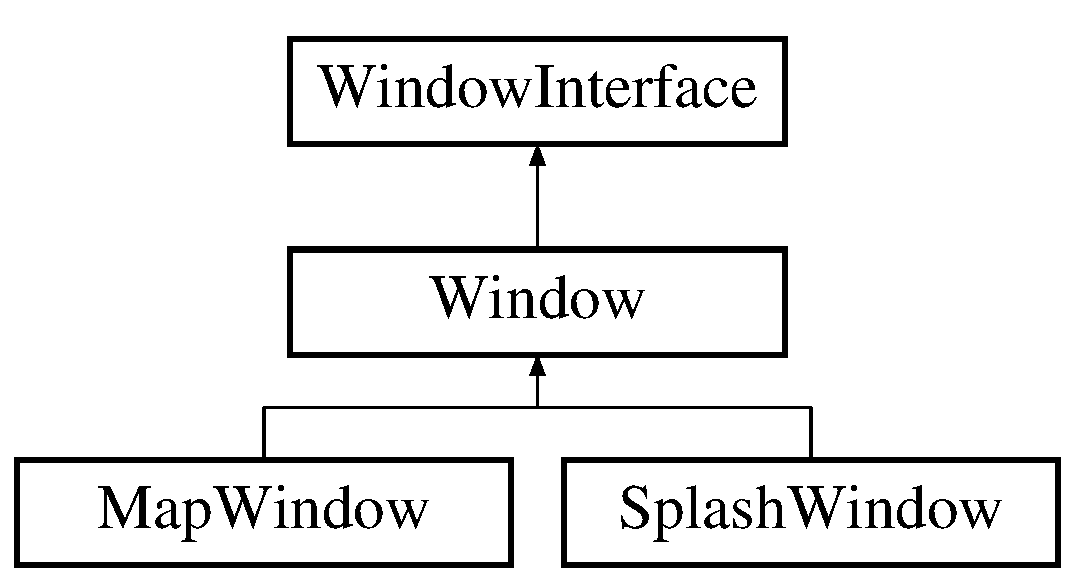
\includegraphics[height=3.000000cm]{classWindowInterface}
\end{center}
\end{figure}
\subsection*{Public Member Functions}
\begin{DoxyCompactItemize}
\item 
virtual \hyperlink{classWindowInterface_a38329b7b17b5ae765d81e40e8093f4c5}{$\sim$\-Window\-Interface} ()
\item 
virtual void \hyperlink{classWindowInterface_a8277c1eb7d3ae7b3f13e06081ffcf66a}{initialise} (\hyperlink{classGameEngineInterface}{Game\-Engine\-Interface} $\ast$a\-\_\-engine)=0
\item 
virtual void \hyperlink{classWindowInterface_afeaed24b8e350acb196964106f2a0146}{destroy} (void)=0
\item 
virtual \hyperlink{classGameEngineInterface}{Game\-Engine\-Interface} $\ast$ \hyperlink{classWindowInterface_ac5970434199b518109a95a5cb645814a}{get\-Engine} ()=0
\item 
virtual void \hyperlink{classWindowInterface_a874548802028401146c44f7ba3e54d1d}{key\-Down} (unsigned char key)=0
\item 
virtual void \hyperlink{classWindowInterface_aa776c5cf4ef3d93a49613e08c79cab77}{key\-Up} (unsigned char key)=0
\item 
virtual bool \hyperlink{classWindowInterface_ab67d23a3dee052fd5901a87518b86e4d}{get\-Key} (unsigned char key)=0
\item 
virtual void \hyperlink{classWindowInterface_a5e6ba2b8e6560e9e3b74794cfd123d59}{mouse\-Down} (int x, int y, int button)=0
\item 
virtual void \hyperlink{classWindowInterface_a482961a40e4a07d7f7ac81fe62ee7762}{mouse\-Up} (int x, int y, int button)=0
\item 
virtual void \hyperlink{classWindowInterface_a8aa6ce7a663628e3bd0480d4566191d2}{before\-Redraw} ()=0
\item 
virtual void \hyperlink{classWindowInterface_a9baf4b0e9c1fdd73b1fe14af4173c699}{redraw} ()=0
\item 
virtual void \hyperlink{classWindowInterface_a37e350fc8f4a97333400c03e8544b2eb}{after\-Redraw} ()=0
\item 
virtual void \hyperlink{classWindowInterface_aa7109fc50fd3e90b0589bdd2a5e6972e}{resize} (int width, int height)=0
\end{DoxyCompactItemize}


\subsection{Constructor \& Destructor Documentation}
\hypertarget{classWindowInterface_a38329b7b17b5ae765d81e40e8093f4c5}{\index{Window\-Interface@{Window\-Interface}!$\sim$\-Window\-Interface@{$\sim$\-Window\-Interface}}
\index{$\sim$\-Window\-Interface@{$\sim$\-Window\-Interface}!WindowInterface@{Window\-Interface}}
\subsubsection[{$\sim$\-Window\-Interface}]{\setlength{\rightskip}{0pt plus 5cm}virtual Window\-Interface\-::$\sim$\-Window\-Interface (
\begin{DoxyParamCaption}
{}
\end{DoxyParamCaption}
)\hspace{0.3cm}{\ttfamily [inline]}, {\ttfamily [virtual]}}}\label{classWindowInterface_a38329b7b17b5ae765d81e40e8093f4c5}


\subsection{Member Function Documentation}
\hypertarget{classWindowInterface_a37e350fc8f4a97333400c03e8544b2eb}{\index{Window\-Interface@{Window\-Interface}!after\-Redraw@{after\-Redraw}}
\index{after\-Redraw@{after\-Redraw}!WindowInterface@{Window\-Interface}}
\subsubsection[{after\-Redraw}]{\setlength{\rightskip}{0pt plus 5cm}virtual void Window\-Interface\-::after\-Redraw (
\begin{DoxyParamCaption}
{}
\end{DoxyParamCaption}
)\hspace{0.3cm}{\ttfamily [pure virtual]}}}\label{classWindowInterface_a37e350fc8f4a97333400c03e8544b2eb}


Implemented in \hyperlink{classWindow_a05b1d6673e37db442ecd80c54d10e6b7}{Window}.

\hypertarget{classWindowInterface_a8aa6ce7a663628e3bd0480d4566191d2}{\index{Window\-Interface@{Window\-Interface}!before\-Redraw@{before\-Redraw}}
\index{before\-Redraw@{before\-Redraw}!WindowInterface@{Window\-Interface}}
\subsubsection[{before\-Redraw}]{\setlength{\rightskip}{0pt plus 5cm}virtual void Window\-Interface\-::before\-Redraw (
\begin{DoxyParamCaption}
{}
\end{DoxyParamCaption}
)\hspace{0.3cm}{\ttfamily [pure virtual]}}}\label{classWindowInterface_a8aa6ce7a663628e3bd0480d4566191d2}


Implemented in \hyperlink{classWindow_a1344118a395cb2fc48d4a2359372b074}{Window}.

\hypertarget{classWindowInterface_afeaed24b8e350acb196964106f2a0146}{\index{Window\-Interface@{Window\-Interface}!destroy@{destroy}}
\index{destroy@{destroy}!WindowInterface@{Window\-Interface}}
\subsubsection[{destroy}]{\setlength{\rightskip}{0pt plus 5cm}virtual void Window\-Interface\-::destroy (
\begin{DoxyParamCaption}
\item[{void}]{}
\end{DoxyParamCaption}
)\hspace{0.3cm}{\ttfamily [pure virtual]}}}\label{classWindowInterface_afeaed24b8e350acb196964106f2a0146}


Implemented in \hyperlink{classWindow_ae0ed7fd17df30f2d262cb684560e0469}{Window}.

\hypertarget{classWindowInterface_ac5970434199b518109a95a5cb645814a}{\index{Window\-Interface@{Window\-Interface}!get\-Engine@{get\-Engine}}
\index{get\-Engine@{get\-Engine}!WindowInterface@{Window\-Interface}}
\subsubsection[{get\-Engine}]{\setlength{\rightskip}{0pt plus 5cm}virtual {\bf Game\-Engine\-Interface}$\ast$ Window\-Interface\-::get\-Engine (
\begin{DoxyParamCaption}
{}
\end{DoxyParamCaption}
)\hspace{0.3cm}{\ttfamily [pure virtual]}}}\label{classWindowInterface_ac5970434199b518109a95a5cb645814a}


Implemented in \hyperlink{classWindow_a55a6e31e36665bd3bcffcd844f5f0385}{Window}.

\hypertarget{classWindowInterface_ab67d23a3dee052fd5901a87518b86e4d}{\index{Window\-Interface@{Window\-Interface}!get\-Key@{get\-Key}}
\index{get\-Key@{get\-Key}!WindowInterface@{Window\-Interface}}
\subsubsection[{get\-Key}]{\setlength{\rightskip}{0pt plus 5cm}virtual bool Window\-Interface\-::get\-Key (
\begin{DoxyParamCaption}
\item[{unsigned char}]{key}
\end{DoxyParamCaption}
)\hspace{0.3cm}{\ttfamily [pure virtual]}}}\label{classWindowInterface_ab67d23a3dee052fd5901a87518b86e4d}


Implemented in \hyperlink{classWindow_ac0927d0b89776959c4a95dd6737f841f}{Window}.

\hypertarget{classWindowInterface_a8277c1eb7d3ae7b3f13e06081ffcf66a}{\index{Window\-Interface@{Window\-Interface}!initialise@{initialise}}
\index{initialise@{initialise}!WindowInterface@{Window\-Interface}}
\subsubsection[{initialise}]{\setlength{\rightskip}{0pt plus 5cm}virtual void Window\-Interface\-::initialise (
\begin{DoxyParamCaption}
\item[{{\bf Game\-Engine\-Interface} $\ast$}]{a\-\_\-engine}
\end{DoxyParamCaption}
)\hspace{0.3cm}{\ttfamily [pure virtual]}}}\label{classWindowInterface_a8277c1eb7d3ae7b3f13e06081ffcf66a}


Implemented in \hyperlink{classWindow_a3dcd22169bd4d40f4b35eafdea31f6dd}{Window}, and \hyperlink{classMapWindow_affdeec7b3b899c38f16d04d170970e70}{Map\-Window}.

\hypertarget{classWindowInterface_a874548802028401146c44f7ba3e54d1d}{\index{Window\-Interface@{Window\-Interface}!key\-Down@{key\-Down}}
\index{key\-Down@{key\-Down}!WindowInterface@{Window\-Interface}}
\subsubsection[{key\-Down}]{\setlength{\rightskip}{0pt plus 5cm}virtual void Window\-Interface\-::key\-Down (
\begin{DoxyParamCaption}
\item[{unsigned char}]{key}
\end{DoxyParamCaption}
)\hspace{0.3cm}{\ttfamily [pure virtual]}}}\label{classWindowInterface_a874548802028401146c44f7ba3e54d1d}


Implemented in \hyperlink{classWindow_a25a5308909ec422bebb480c803e1233c}{Window}, and \hyperlink{classMapWindow_a289795e503a5aa600e4091f5aa8b0b8c}{Map\-Window}.

\hypertarget{classWindowInterface_aa776c5cf4ef3d93a49613e08c79cab77}{\index{Window\-Interface@{Window\-Interface}!key\-Up@{key\-Up}}
\index{key\-Up@{key\-Up}!WindowInterface@{Window\-Interface}}
\subsubsection[{key\-Up}]{\setlength{\rightskip}{0pt plus 5cm}virtual void Window\-Interface\-::key\-Up (
\begin{DoxyParamCaption}
\item[{unsigned char}]{key}
\end{DoxyParamCaption}
)\hspace{0.3cm}{\ttfamily [pure virtual]}}}\label{classWindowInterface_aa776c5cf4ef3d93a49613e08c79cab77}


Implemented in \hyperlink{classWindow_a249f5a9513be00e59428a1df37502c63}{Window}.

\hypertarget{classWindowInterface_a5e6ba2b8e6560e9e3b74794cfd123d59}{\index{Window\-Interface@{Window\-Interface}!mouse\-Down@{mouse\-Down}}
\index{mouse\-Down@{mouse\-Down}!WindowInterface@{Window\-Interface}}
\subsubsection[{mouse\-Down}]{\setlength{\rightskip}{0pt plus 5cm}virtual void Window\-Interface\-::mouse\-Down (
\begin{DoxyParamCaption}
\item[{int}]{x, }
\item[{int}]{y, }
\item[{int}]{button}
\end{DoxyParamCaption}
)\hspace{0.3cm}{\ttfamily [pure virtual]}}}\label{classWindowInterface_a5e6ba2b8e6560e9e3b74794cfd123d59}


Implemented in \hyperlink{classWindow_ace3bd5e6614510fce97263eccc35c0ab}{Window}.

\hypertarget{classWindowInterface_a482961a40e4a07d7f7ac81fe62ee7762}{\index{Window\-Interface@{Window\-Interface}!mouse\-Up@{mouse\-Up}}
\index{mouse\-Up@{mouse\-Up}!WindowInterface@{Window\-Interface}}
\subsubsection[{mouse\-Up}]{\setlength{\rightskip}{0pt plus 5cm}virtual void Window\-Interface\-::mouse\-Up (
\begin{DoxyParamCaption}
\item[{int}]{x, }
\item[{int}]{y, }
\item[{int}]{button}
\end{DoxyParamCaption}
)\hspace{0.3cm}{\ttfamily [pure virtual]}}}\label{classWindowInterface_a482961a40e4a07d7f7ac81fe62ee7762}


Implemented in \hyperlink{classWindow_a2e2c7592975405513a05a2da6a512b1c}{Window}.

\hypertarget{classWindowInterface_a9baf4b0e9c1fdd73b1fe14af4173c699}{\index{Window\-Interface@{Window\-Interface}!redraw@{redraw}}
\index{redraw@{redraw}!WindowInterface@{Window\-Interface}}
\subsubsection[{redraw}]{\setlength{\rightskip}{0pt plus 5cm}virtual void Window\-Interface\-::redraw (
\begin{DoxyParamCaption}
{}
\end{DoxyParamCaption}
)\hspace{0.3cm}{\ttfamily [pure virtual]}}}\label{classWindowInterface_a9baf4b0e9c1fdd73b1fe14af4173c699}


Implemented in \hyperlink{classWindow_aa8b52b7035a78ef960c194c9bb4a7c36}{Window}, \hyperlink{classMapWindow_a5759338c3758b2a3252ffc691958dff8}{Map\-Window}, and \hyperlink{classSplashWindow_aad27778951eb9dd5dbb03635f2bda114}{Splash\-Window}.

\hypertarget{classWindowInterface_aa7109fc50fd3e90b0589bdd2a5e6972e}{\index{Window\-Interface@{Window\-Interface}!resize@{resize}}
\index{resize@{resize}!WindowInterface@{Window\-Interface}}
\subsubsection[{resize}]{\setlength{\rightskip}{0pt plus 5cm}virtual void Window\-Interface\-::resize (
\begin{DoxyParamCaption}
\item[{int}]{width, }
\item[{int}]{height}
\end{DoxyParamCaption}
)\hspace{0.3cm}{\ttfamily [pure virtual]}}}\label{classWindowInterface_aa7109fc50fd3e90b0589bdd2a5e6972e}


Implemented in \hyperlink{classWindow_a6e4274c73728009132b7e0dfad42a8de}{Window}.



The documentation for this class was generated from the following file\-:\begin{DoxyCompactItemize}
\item 
\hyperlink{window__interface_8h}{window\-\_\-interface.\-h}\end{DoxyCompactItemize}

\hypertarget{classWindowManager}{\section{Window\-Manager Class Reference}
\label{classWindowManager}\index{Window\-Manager@{Window\-Manager}}
}


{\ttfamily \#include $<$window\-\_\-manager.\-h$>$}

Inheritance diagram for Window\-Manager\-:\begin{figure}[H]
\begin{center}
\leavevmode
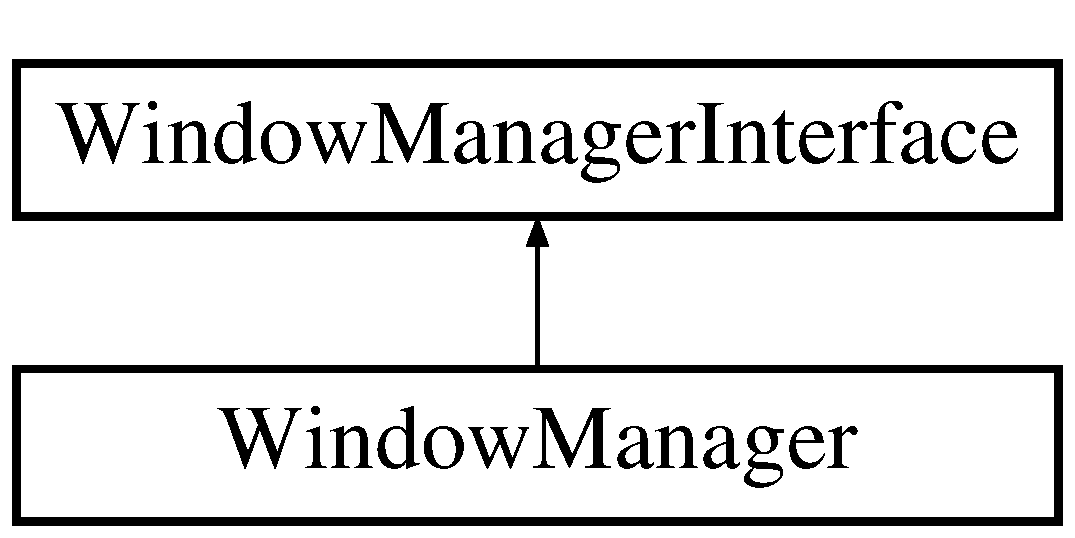
\includegraphics[height=2.000000cm]{classWindowManager}
\end{center}
\end{figure}
\subsection*{Public Member Functions}
\begin{DoxyCompactItemize}
\item 
void \hyperlink{classWindowManager_a8a4daf5be17d22415df9b5c9a577ebe0}{initialise} (\hyperlink{classGameEngineInterface}{Game\-Engine\-Interface} $\ast$engine)
\item 
void \hyperlink{classWindowManager_a1686c44231c43bff5c8b262d2f0b7c86}{add\-Window} (\hyperlink{classWindowInterface}{Window\-Interface} $\ast$win)
\item 
void \hyperlink{classWindowManager_a42dae7b3b11730f2a4fe629cdc22ee6d}{pop\-Window} ()
\item 
void \hyperlink{classWindowManager_af5e3a6217eaba1bbbf4b7f1d45707467}{replace\-Window} (\hyperlink{classWindowInterface}{Window\-Interface} $\ast$win)
\item 
\hyperlink{classWindowInterface}{Window\-Interface} $\ast$ \hyperlink{classWindowManager_aa6e650ff5d24dab3930abb578a3a3e63}{get\-Active} ()
\end{DoxyCompactItemize}
\subsection*{Private Attributes}
\begin{DoxyCompactItemize}
\item 
\hyperlink{classGameEngineInterface}{Game\-Engine\-Interface} $\ast$ \hyperlink{classWindowManager_ae1fb8500f2391518ba8c7b2cfb6f30f7}{m\-\_\-engine}
\item 
std\-::vector$<$ \hyperlink{classWindowInterface}{Window\-Interface} $\ast$ $>$ \hyperlink{classWindowManager_ad3b8bc0fa911812f00a871c195944c65}{m\-\_\-windows}
\end{DoxyCompactItemize}


\subsection{Member Function Documentation}
\hypertarget{classWindowManager_a1686c44231c43bff5c8b262d2f0b7c86}{\index{Window\-Manager@{Window\-Manager}!add\-Window@{add\-Window}}
\index{add\-Window@{add\-Window}!WindowManager@{Window\-Manager}}
\subsubsection[{add\-Window}]{\setlength{\rightskip}{0pt plus 5cm}void Window\-Manager\-::add\-Window (
\begin{DoxyParamCaption}
\item[{{\bf Window\-Interface} $\ast$}]{win}
\end{DoxyParamCaption}
)\hspace{0.3cm}{\ttfamily [inline]}, {\ttfamily [virtual]}}}\label{classWindowManager_a1686c44231c43bff5c8b262d2f0b7c86}


Implements \hyperlink{classWindowManagerInterface_aac36e2671a3d60b6b14469176da14c70}{Window\-Manager\-Interface}.

\hypertarget{classWindowManager_aa6e650ff5d24dab3930abb578a3a3e63}{\index{Window\-Manager@{Window\-Manager}!get\-Active@{get\-Active}}
\index{get\-Active@{get\-Active}!WindowManager@{Window\-Manager}}
\subsubsection[{get\-Active}]{\setlength{\rightskip}{0pt plus 5cm}{\bf Window\-Interface} $\ast$ Window\-Manager\-::get\-Active (
\begin{DoxyParamCaption}
{}
\end{DoxyParamCaption}
)\hspace{0.3cm}{\ttfamily [virtual]}}}\label{classWindowManager_aa6e650ff5d24dab3930abb578a3a3e63}


Implements \hyperlink{classWindowManagerInterface_a67c7bd0f3376cd9bd9be6970902d871a}{Window\-Manager\-Interface}.

\hypertarget{classWindowManager_a8a4daf5be17d22415df9b5c9a577ebe0}{\index{Window\-Manager@{Window\-Manager}!initialise@{initialise}}
\index{initialise@{initialise}!WindowManager@{Window\-Manager}}
\subsubsection[{initialise}]{\setlength{\rightskip}{0pt plus 5cm}void Window\-Manager\-::initialise (
\begin{DoxyParamCaption}
\item[{{\bf Game\-Engine\-Interface} $\ast$}]{engine}
\end{DoxyParamCaption}
)\hspace{0.3cm}{\ttfamily [virtual]}}}\label{classWindowManager_a8a4daf5be17d22415df9b5c9a577ebe0}


Implements \hyperlink{classWindowManagerInterface_aa5332643f381faff81e0bb4af1c1941e}{Window\-Manager\-Interface}.

\hypertarget{classWindowManager_a42dae7b3b11730f2a4fe629cdc22ee6d}{\index{Window\-Manager@{Window\-Manager}!pop\-Window@{pop\-Window}}
\index{pop\-Window@{pop\-Window}!WindowManager@{Window\-Manager}}
\subsubsection[{pop\-Window}]{\setlength{\rightskip}{0pt plus 5cm}void Window\-Manager\-::pop\-Window (
\begin{DoxyParamCaption}
{}
\end{DoxyParamCaption}
)\hspace{0.3cm}{\ttfamily [virtual]}}}\label{classWindowManager_a42dae7b3b11730f2a4fe629cdc22ee6d}


Implements \hyperlink{classWindowManagerInterface_a4e9b4365650eeb65babbab6ddff30677}{Window\-Manager\-Interface}.

\hypertarget{classWindowManager_af5e3a6217eaba1bbbf4b7f1d45707467}{\index{Window\-Manager@{Window\-Manager}!replace\-Window@{replace\-Window}}
\index{replace\-Window@{replace\-Window}!WindowManager@{Window\-Manager}}
\subsubsection[{replace\-Window}]{\setlength{\rightskip}{0pt plus 5cm}void Window\-Manager\-::replace\-Window (
\begin{DoxyParamCaption}
\item[{{\bf Window\-Interface} $\ast$}]{win}
\end{DoxyParamCaption}
)\hspace{0.3cm}{\ttfamily [virtual]}}}\label{classWindowManager_af5e3a6217eaba1bbbf4b7f1d45707467}


Implements \hyperlink{classWindowManagerInterface_a776651d54dbdcdbe4d09b03f22cb0cdb}{Window\-Manager\-Interface}.



\subsection{Member Data Documentation}
\hypertarget{classWindowManager_ae1fb8500f2391518ba8c7b2cfb6f30f7}{\index{Window\-Manager@{Window\-Manager}!m\-\_\-engine@{m\-\_\-engine}}
\index{m\-\_\-engine@{m\-\_\-engine}!WindowManager@{Window\-Manager}}
\subsubsection[{m\-\_\-engine}]{\setlength{\rightskip}{0pt plus 5cm}{\bf Game\-Engine\-Interface}$\ast$ Window\-Manager\-::m\-\_\-engine\hspace{0.3cm}{\ttfamily [private]}}}\label{classWindowManager_ae1fb8500f2391518ba8c7b2cfb6f30f7}
\hypertarget{classWindowManager_ad3b8bc0fa911812f00a871c195944c65}{\index{Window\-Manager@{Window\-Manager}!m\-\_\-windows@{m\-\_\-windows}}
\index{m\-\_\-windows@{m\-\_\-windows}!WindowManager@{Window\-Manager}}
\subsubsection[{m\-\_\-windows}]{\setlength{\rightskip}{0pt plus 5cm}std\-::vector$<${\bf Window\-Interface}$\ast$$>$ Window\-Manager\-::m\-\_\-windows\hspace{0.3cm}{\ttfamily [private]}}}\label{classWindowManager_ad3b8bc0fa911812f00a871c195944c65}


The documentation for this class was generated from the following files\-:\begin{DoxyCompactItemize}
\item 
\hyperlink{window__manager_8h}{window\-\_\-manager.\-h}\item 
\hyperlink{window__manager_8cpp}{window\-\_\-manager.\-cpp}\end{DoxyCompactItemize}

\hypertarget{classWindowManagerInterface}{\section{Window\-Manager\-Interface Class Reference}
\label{classWindowManagerInterface}\index{Window\-Manager\-Interface@{Window\-Manager\-Interface}}
}


{\ttfamily \#include $<$window\-\_\-manager\-\_\-interface.\-h$>$}

Inheritance diagram for Window\-Manager\-Interface\-:\begin{figure}[H]
\begin{center}
\leavevmode
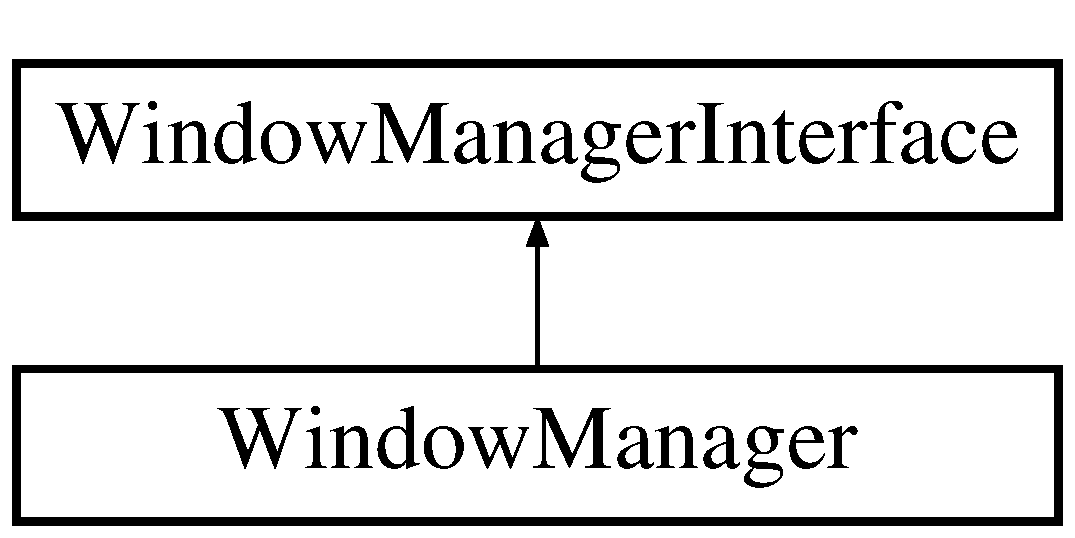
\includegraphics[height=2.000000cm]{classWindowManagerInterface}
\end{center}
\end{figure}
\subsection*{Public Member Functions}
\begin{DoxyCompactItemize}
\item 
virtual \hyperlink{classWindowManagerInterface_aec641c997562e0ca7af76c723ccf7330}{$\sim$\-Window\-Manager\-Interface} ()
\item 
virtual void \hyperlink{classWindowManagerInterface_aa5332643f381faff81e0bb4af1c1941e}{initialise} (\hyperlink{classGameEngineInterface}{Game\-Engine\-Interface} $\ast$engine)=0
\item 
virtual void \hyperlink{classWindowManagerInterface_aac36e2671a3d60b6b14469176da14c70}{add\-Window} (\hyperlink{classWindowInterface}{Window\-Interface} $\ast$win)=0
\item 
virtual void \hyperlink{classWindowManagerInterface_a4e9b4365650eeb65babbab6ddff30677}{pop\-Window} ()=0
\item 
virtual void \hyperlink{classWindowManagerInterface_a776651d54dbdcdbe4d09b03f22cb0cdb}{replace\-Window} (\hyperlink{classWindowInterface}{Window\-Interface} $\ast$win)=0
\item 
virtual \hyperlink{classWindowInterface}{Window\-Interface} $\ast$ \hyperlink{classWindowManagerInterface_a67c7bd0f3376cd9bd9be6970902d871a}{get\-Active} ()=0
\end{DoxyCompactItemize}


\subsection{Constructor \& Destructor Documentation}
\hypertarget{classWindowManagerInterface_aec641c997562e0ca7af76c723ccf7330}{\index{Window\-Manager\-Interface@{Window\-Manager\-Interface}!$\sim$\-Window\-Manager\-Interface@{$\sim$\-Window\-Manager\-Interface}}
\index{$\sim$\-Window\-Manager\-Interface@{$\sim$\-Window\-Manager\-Interface}!WindowManagerInterface@{Window\-Manager\-Interface}}
\subsubsection[{$\sim$\-Window\-Manager\-Interface}]{\setlength{\rightskip}{0pt plus 5cm}virtual Window\-Manager\-Interface\-::$\sim$\-Window\-Manager\-Interface (
\begin{DoxyParamCaption}
{}
\end{DoxyParamCaption}
)\hspace{0.3cm}{\ttfamily [inline]}, {\ttfamily [virtual]}}}\label{classWindowManagerInterface_aec641c997562e0ca7af76c723ccf7330}


\subsection{Member Function Documentation}
\hypertarget{classWindowManagerInterface_aac36e2671a3d60b6b14469176da14c70}{\index{Window\-Manager\-Interface@{Window\-Manager\-Interface}!add\-Window@{add\-Window}}
\index{add\-Window@{add\-Window}!WindowManagerInterface@{Window\-Manager\-Interface}}
\subsubsection[{add\-Window}]{\setlength{\rightskip}{0pt plus 5cm}virtual void Window\-Manager\-Interface\-::add\-Window (
\begin{DoxyParamCaption}
\item[{{\bf Window\-Interface} $\ast$}]{win}
\end{DoxyParamCaption}
)\hspace{0.3cm}{\ttfamily [pure virtual]}}}\label{classWindowManagerInterface_aac36e2671a3d60b6b14469176da14c70}


Implemented in \hyperlink{classWindowManager_a1686c44231c43bff5c8b262d2f0b7c86}{Window\-Manager}.

\hypertarget{classWindowManagerInterface_a67c7bd0f3376cd9bd9be6970902d871a}{\index{Window\-Manager\-Interface@{Window\-Manager\-Interface}!get\-Active@{get\-Active}}
\index{get\-Active@{get\-Active}!WindowManagerInterface@{Window\-Manager\-Interface}}
\subsubsection[{get\-Active}]{\setlength{\rightskip}{0pt plus 5cm}virtual {\bf Window\-Interface}$\ast$ Window\-Manager\-Interface\-::get\-Active (
\begin{DoxyParamCaption}
{}
\end{DoxyParamCaption}
)\hspace{0.3cm}{\ttfamily [pure virtual]}}}\label{classWindowManagerInterface_a67c7bd0f3376cd9bd9be6970902d871a}


Implemented in \hyperlink{classWindowManager_aa6e650ff5d24dab3930abb578a3a3e63}{Window\-Manager}.

\hypertarget{classWindowManagerInterface_aa5332643f381faff81e0bb4af1c1941e}{\index{Window\-Manager\-Interface@{Window\-Manager\-Interface}!initialise@{initialise}}
\index{initialise@{initialise}!WindowManagerInterface@{Window\-Manager\-Interface}}
\subsubsection[{initialise}]{\setlength{\rightskip}{0pt plus 5cm}virtual void Window\-Manager\-Interface\-::initialise (
\begin{DoxyParamCaption}
\item[{{\bf Game\-Engine\-Interface} $\ast$}]{engine}
\end{DoxyParamCaption}
)\hspace{0.3cm}{\ttfamily [pure virtual]}}}\label{classWindowManagerInterface_aa5332643f381faff81e0bb4af1c1941e}


Implemented in \hyperlink{classWindowManager_a8a4daf5be17d22415df9b5c9a577ebe0}{Window\-Manager}.

\hypertarget{classWindowManagerInterface_a4e9b4365650eeb65babbab6ddff30677}{\index{Window\-Manager\-Interface@{Window\-Manager\-Interface}!pop\-Window@{pop\-Window}}
\index{pop\-Window@{pop\-Window}!WindowManagerInterface@{Window\-Manager\-Interface}}
\subsubsection[{pop\-Window}]{\setlength{\rightskip}{0pt plus 5cm}virtual void Window\-Manager\-Interface\-::pop\-Window (
\begin{DoxyParamCaption}
{}
\end{DoxyParamCaption}
)\hspace{0.3cm}{\ttfamily [pure virtual]}}}\label{classWindowManagerInterface_a4e9b4365650eeb65babbab6ddff30677}


Implemented in \hyperlink{classWindowManager_a42dae7b3b11730f2a4fe629cdc22ee6d}{Window\-Manager}.

\hypertarget{classWindowManagerInterface_a776651d54dbdcdbe4d09b03f22cb0cdb}{\index{Window\-Manager\-Interface@{Window\-Manager\-Interface}!replace\-Window@{replace\-Window}}
\index{replace\-Window@{replace\-Window}!WindowManagerInterface@{Window\-Manager\-Interface}}
\subsubsection[{replace\-Window}]{\setlength{\rightskip}{0pt plus 5cm}virtual void Window\-Manager\-Interface\-::replace\-Window (
\begin{DoxyParamCaption}
\item[{{\bf Window\-Interface} $\ast$}]{win}
\end{DoxyParamCaption}
)\hspace{0.3cm}{\ttfamily [pure virtual]}}}\label{classWindowManagerInterface_a776651d54dbdcdbe4d09b03f22cb0cdb}


Implemented in \hyperlink{classWindowManager_af5e3a6217eaba1bbbf4b7f1d45707467}{Window\-Manager}.



The documentation for this class was generated from the following file\-:\begin{DoxyCompactItemize}
\item 
\hyperlink{window__manager__interface_8h}{window\-\_\-manager\-\_\-interface.\-h}\end{DoxyCompactItemize}

\chapter{File Documentation}
\hypertarget{algorithm_8cpp}{\section{algorithm.\-cpp File Reference}
\label{algorithm_8cpp}\index{algorithm.\-cpp@{algorithm.\-cpp}}
}
{\ttfamily \#include \char`\"{}algorithm.\-h\char`\"{}}\\*
{\ttfamily \#include \char`\"{}gameengine.\-h\char`\"{}}\\*
{\ttfamily \#include $<$cstdio$>$}\\*
{\ttfamily \#include $<$cstdlib$>$}\\*
{\ttfamily \#include $<$queue$>$}\\*
{\ttfamily \#include $<$ctime$>$}\\*
{\ttfamily \#include $<$unistd.\-h$>$}\\*
{\ttfamily \#include $<$vector$>$}\\*
{\ttfamily \#include $<$map$>$}\\*
{\ttfamily \#include $<$iostream$>$}\\*

\hypertarget{algorithm_8h}{\section{algorithm.\-h File Reference}
\label{algorithm_8h}\index{algorithm.\-h@{algorithm.\-h}}
}
{\ttfamily \#include $<$vector$>$}\\*

\hypertarget{collider__component_8h}{\section{collider\-\_\-component.\-h File Reference}
\label{collider__component_8h}\index{collider\-\_\-component.\-h@{collider\-\_\-component.\-h}}
}
\subsection*{Classes}
\begin{DoxyCompactItemize}
\item 
struct \hyperlink{structColliderComponent}{Collider\-Component}
\end{DoxyCompactItemize}

\hypertarget{color_8cpp}{\section{color.\-cpp File Reference}
\label{color_8cpp}\index{color.\-cpp@{color.\-cpp}}
}
{\ttfamily \#include \char`\"{}color.\-h\char`\"{}}\\*

\hypertarget{color_8h}{\section{color.\-h File Reference}
\label{color_8h}\index{color.\-h@{color.\-h}}
}
\subsection*{Classes}
\begin{DoxyCompactItemize}
\item 
class \hyperlink{classColor}{Color}
\end{DoxyCompactItemize}
\subsection*{Enumerations}
\begin{DoxyCompactItemize}
\item 
enum \hyperlink{color_8h_af90824509586333cf45ce757d2711ce3}{C\-O\-L\-O\-R} \{ \\*
\hyperlink{color_8h_af90824509586333cf45ce757d2711ce3af80f9a890089d211842d59625e561f88}{R\-E\-D}, 
\hyperlink{color_8h_af90824509586333cf45ce757d2711ce3aa60bd322f93178d68184e30e162571ca}{G\-R\-E\-E\-N}, 
\hyperlink{color_8h_af90824509586333cf45ce757d2711ce3a35d6719cb4d7577c031b3d79057a1b79}{B\-L\-U\-E}, 
\hyperlink{color_8h_af90824509586333cf45ce757d2711ce3a283fc479650da98250635b9c3c0e7e50}{W\-H\-I\-T\-E}, 
\\*
\hyperlink{color_8h_af90824509586333cf45ce757d2711ce3af77fb67151d0c18d397069ad8c271ba3}{B\-L\-A\-C\-K}, 
\hyperlink{color_8h_af90824509586333cf45ce757d2711ce3a38566822dbd9408c447abfd3ed4a85d2}{G\-R\-E\-Y}
 \}
\end{DoxyCompactItemize}


\subsection{Enumeration Type Documentation}
\hypertarget{color_8h_af90824509586333cf45ce757d2711ce3}{\index{color.\-h@{color.\-h}!C\-O\-L\-O\-R@{C\-O\-L\-O\-R}}
\index{C\-O\-L\-O\-R@{C\-O\-L\-O\-R}!color.h@{color.\-h}}
\subsubsection[{C\-O\-L\-O\-R}]{\setlength{\rightskip}{0pt plus 5cm}enum {\bf C\-O\-L\-O\-R}}}\label{color_8h_af90824509586333cf45ce757d2711ce3}
\begin{Desc}
\item[Enumerator]\par
\begin{description}
\index{R\-E\-D@{R\-E\-D}!color.\-h@{color.\-h}}\index{color.\-h@{color.\-h}!R\-E\-D@{R\-E\-D}}\item[{\em 
\hypertarget{color_8h_af90824509586333cf45ce757d2711ce3af80f9a890089d211842d59625e561f88}{R\-E\-D}\label{color_8h_af90824509586333cf45ce757d2711ce3af80f9a890089d211842d59625e561f88}
}]\index{G\-R\-E\-E\-N@{G\-R\-E\-E\-N}!color.\-h@{color.\-h}}\index{color.\-h@{color.\-h}!G\-R\-E\-E\-N@{G\-R\-E\-E\-N}}\item[{\em 
\hypertarget{color_8h_af90824509586333cf45ce757d2711ce3aa60bd322f93178d68184e30e162571ca}{G\-R\-E\-E\-N}\label{color_8h_af90824509586333cf45ce757d2711ce3aa60bd322f93178d68184e30e162571ca}
}]\index{B\-L\-U\-E@{B\-L\-U\-E}!color.\-h@{color.\-h}}\index{color.\-h@{color.\-h}!B\-L\-U\-E@{B\-L\-U\-E}}\item[{\em 
\hypertarget{color_8h_af90824509586333cf45ce757d2711ce3a35d6719cb4d7577c031b3d79057a1b79}{B\-L\-U\-E}\label{color_8h_af90824509586333cf45ce757d2711ce3a35d6719cb4d7577c031b3d79057a1b79}
}]\index{W\-H\-I\-T\-E@{W\-H\-I\-T\-E}!color.\-h@{color.\-h}}\index{color.\-h@{color.\-h}!W\-H\-I\-T\-E@{W\-H\-I\-T\-E}}\item[{\em 
\hypertarget{color_8h_af90824509586333cf45ce757d2711ce3a283fc479650da98250635b9c3c0e7e50}{W\-H\-I\-T\-E}\label{color_8h_af90824509586333cf45ce757d2711ce3a283fc479650da98250635b9c3c0e7e50}
}]\index{B\-L\-A\-C\-K@{B\-L\-A\-C\-K}!color.\-h@{color.\-h}}\index{color.\-h@{color.\-h}!B\-L\-A\-C\-K@{B\-L\-A\-C\-K}}\item[{\em 
\hypertarget{color_8h_af90824509586333cf45ce757d2711ce3af77fb67151d0c18d397069ad8c271ba3}{B\-L\-A\-C\-K}\label{color_8h_af90824509586333cf45ce757d2711ce3af77fb67151d0c18d397069ad8c271ba3}
}]\index{G\-R\-E\-Y@{G\-R\-E\-Y}!color.\-h@{color.\-h}}\index{color.\-h@{color.\-h}!G\-R\-E\-Y@{G\-R\-E\-Y}}\item[{\em 
\hypertarget{color_8h_af90824509586333cf45ce757d2711ce3a38566822dbd9408c447abfd3ed4a85d2}{G\-R\-E\-Y}\label{color_8h_af90824509586333cf45ce757d2711ce3a38566822dbd9408c447abfd3ed4a85d2}
}]\end{description}
\end{Desc}

\hypertarget{combat__system_8cpp}{\section{combat\-\_\-system.\-cpp File Reference}
\label{combat__system_8cpp}\index{combat\-\_\-system.\-cpp@{combat\-\_\-system.\-cpp}}
}
{\ttfamily \#include \char`\"{}combat\-\_\-system.\-h\char`\"{}}\\*
{\ttfamily \#include $<$iostream$>$}\\*

\hypertarget{combat__system_8h}{\section{combat\-\_\-system.\-h File Reference}
\label{combat__system_8h}\index{combat\-\_\-system.\-h@{combat\-\_\-system.\-h}}
}
{\ttfamily \#include \char`\"{}game\-\_\-system\-\_\-base.\-h\char`\"{}}\\*
\subsection*{Classes}
\begin{DoxyCompactItemize}
\item 
class \hyperlink{classCombatSystem}{Combat\-System}
\end{DoxyCompactItemize}

\hypertarget{component__manager_8cpp}{\section{component\-\_\-manager.\-cpp File Reference}
\label{component__manager_8cpp}\index{component\-\_\-manager.\-cpp@{component\-\_\-manager.\-cpp}}
}
{\ttfamily \#include \char`\"{}component\-\_\-manager.\-h\char`\"{}}\\*
{\ttfamily \#include \char`\"{}entity.\-h\char`\"{}}\\*
{\ttfamily \#include $<$map$>$}\\*

\hypertarget{component__manager_8h}{\section{component\-\_\-manager.\-h File Reference}
\label{component__manager_8h}\index{component\-\_\-manager.\-h@{component\-\_\-manager.\-h}}
}
{\ttfamily \#include \char`\"{}component\-\_\-manager\-\_\-interface.\-h\char`\"{}}\\*
{\ttfamily \#include \char`\"{}entity.\-h\char`\"{}}\\*
{\ttfamily \#include $<$map$>$}\\*
\subsection*{Classes}
\begin{DoxyCompactItemize}
\item 
class \hyperlink{classComponentManager}{Component\-Manager$<$ T $>$}
\end{DoxyCompactItemize}

\hypertarget{component__manager__interface_8h}{\section{component\-\_\-manager\-\_\-interface.\-h File Reference}
\label{component__manager__interface_8h}\index{component\-\_\-manager\-\_\-interface.\-h@{component\-\_\-manager\-\_\-interface.\-h}}
}
{\ttfamily \#include \char`\"{}entity.\-h\char`\"{}}\\*
{\ttfamily \#include $<$map$>$}\\*
\subsection*{Classes}
\begin{DoxyCompactItemize}
\item 
class \hyperlink{classComponentManagerInterface}{Component\-Manager\-Interface$<$ T $>$}
\end{DoxyCompactItemize}

\hypertarget{config__manager_8cpp}{\section{config\-\_\-manager.\-cpp File Reference}
\label{config__manager_8cpp}\index{config\-\_\-manager.\-cpp@{config\-\_\-manager.\-cpp}}
}
{\ttfamily \#include $<$config\-\_\-manager.\-h$>$}\\*
{\ttfamily \#include $<$fstream$>$}\\*
{\ttfamily \#include $<$iostream$>$}\\*
{\ttfamily \#include $<$sstream$>$}\\*

\hypertarget{config__manager_8h}{\section{config\-\_\-manager.\-h File Reference}
\label{config__manager_8h}\index{config\-\_\-manager.\-h@{config\-\_\-manager.\-h}}
}
{\ttfamily \#include $<$map$>$}\\*
{\ttfamily \#include $<$string$>$}\\*
\subsection*{Classes}
\begin{DoxyCompactItemize}
\item 
struct \hyperlink{structTagValue}{Tag\-Value}
\item 
class \hyperlink{classConfigManager}{Config\-Manager}
\end{DoxyCompactItemize}

\hypertarget{entity_8cpp}{\section{entity.\-cpp File Reference}
\label{entity_8cpp}\index{entity.\-cpp@{entity.\-cpp}}
}
{\ttfamily \#include \char`\"{}entity.\-h\char`\"{}}\\*
\subsection*{Functions}
\begin{DoxyCompactItemize}
\item 
bool \hyperlink{entity_8cpp_a14c0b7c3e6659d87c47ed69dcfe80f43}{operator$<$} (const \hyperlink{classEntity}{Entity} \&lhs, const \hyperlink{classEntity}{Entity} \&rhs)
\end{DoxyCompactItemize}


\subsection{Function Documentation}
\hypertarget{entity_8cpp_a14c0b7c3e6659d87c47ed69dcfe80f43}{\index{entity.\-cpp@{entity.\-cpp}!operator$<$@{operator$<$}}
\index{operator$<$@{operator$<$}!entity.cpp@{entity.\-cpp}}
\subsubsection[{operator$<$}]{\setlength{\rightskip}{0pt plus 5cm}bool operator$<$ (
\begin{DoxyParamCaption}
\item[{const {\bf Entity} \&}]{lhs, }
\item[{const {\bf Entity} \&}]{rhs}
\end{DoxyParamCaption}
)}}\label{entity_8cpp_a14c0b7c3e6659d87c47ed69dcfe80f43}

\hypertarget{entity_8h}{\section{entity.\-h File Reference}
\label{entity_8h}\index{entity.\-h@{entity.\-h}}
}
{\ttfamily \#include $<$set$>$}\\*
{\ttfamily \#include $<$string$>$}\\*
\subsection*{Classes}
\begin{DoxyCompactItemize}
\item 
class \hyperlink{classEntity}{Entity}
\end{DoxyCompactItemize}
\subsection*{Typedefs}
\begin{DoxyCompactItemize}
\item 
typedef unsigned long \hyperlink{entity_8h_a3812b46f7256476cf244cbc0f4a3bde9}{Entity\-Id}
\end{DoxyCompactItemize}
\subsection*{Enumerations}
\begin{DoxyCompactItemize}
\item 
enum \hyperlink{entity_8h_a305263dd89ad9fde1863aece00907351}{Tag} \{ \hyperlink{entity_8h_a305263dd89ad9fde1863aece00907351ade5dc3e0dbd007d995ed3e37bde5ce7e}{P\-L\-A\-Y\-E\-R}, 
\hyperlink{entity_8h_a305263dd89ad9fde1863aece00907351af496eff98f9bb45646f2c88ea331998e}{M\-O\-N\-S\-T\-E\-R}, 
\hyperlink{entity_8h_a305263dd89ad9fde1863aece00907351afca2faad41310c7e71ec303ef789c53a}{W\-A\-L\-L}
 \}
\end{DoxyCompactItemize}
\subsection*{Functions}
\begin{DoxyCompactItemize}
\item 
bool \hyperlink{entity_8h_a14c0b7c3e6659d87c47ed69dcfe80f43}{operator$<$} (const \hyperlink{classEntity}{Entity} \&lhs, const \hyperlink{classEntity}{Entity} \&rhs)
\end{DoxyCompactItemize}


\subsection{Typedef Documentation}
\hypertarget{entity_8h_a3812b46f7256476cf244cbc0f4a3bde9}{\index{entity.\-h@{entity.\-h}!Entity\-Id@{Entity\-Id}}
\index{Entity\-Id@{Entity\-Id}!entity.h@{entity.\-h}}
\subsubsection[{Entity\-Id}]{\setlength{\rightskip}{0pt plus 5cm}typedef unsigned long {\bf Entity\-Id}}}\label{entity_8h_a3812b46f7256476cf244cbc0f4a3bde9}


\subsection{Enumeration Type Documentation}
\hypertarget{entity_8h_a305263dd89ad9fde1863aece00907351}{\index{entity.\-h@{entity.\-h}!Tag@{Tag}}
\index{Tag@{Tag}!entity.h@{entity.\-h}}
\subsubsection[{Tag}]{\setlength{\rightskip}{0pt plus 5cm}enum {\bf Tag}}}\label{entity_8h_a305263dd89ad9fde1863aece00907351}
\begin{Desc}
\item[Enumerator]\par
\begin{description}
\index{P\-L\-A\-Y\-E\-R@{P\-L\-A\-Y\-E\-R}!entity.\-h@{entity.\-h}}\index{entity.\-h@{entity.\-h}!P\-L\-A\-Y\-E\-R@{P\-L\-A\-Y\-E\-R}}\item[{\em 
\hypertarget{entity_8h_a305263dd89ad9fde1863aece00907351ade5dc3e0dbd007d995ed3e37bde5ce7e}{P\-L\-A\-Y\-E\-R}\label{entity_8h_a305263dd89ad9fde1863aece00907351ade5dc3e0dbd007d995ed3e37bde5ce7e}
}]\index{M\-O\-N\-S\-T\-E\-R@{M\-O\-N\-S\-T\-E\-R}!entity.\-h@{entity.\-h}}\index{entity.\-h@{entity.\-h}!M\-O\-N\-S\-T\-E\-R@{M\-O\-N\-S\-T\-E\-R}}\item[{\em 
\hypertarget{entity_8h_a305263dd89ad9fde1863aece00907351af496eff98f9bb45646f2c88ea331998e}{M\-O\-N\-S\-T\-E\-R}\label{entity_8h_a305263dd89ad9fde1863aece00907351af496eff98f9bb45646f2c88ea331998e}
}]\index{W\-A\-L\-L@{W\-A\-L\-L}!entity.\-h@{entity.\-h}}\index{entity.\-h@{entity.\-h}!W\-A\-L\-L@{W\-A\-L\-L}}\item[{\em 
\hypertarget{entity_8h_a305263dd89ad9fde1863aece00907351afca2faad41310c7e71ec303ef789c53a}{W\-A\-L\-L}\label{entity_8h_a305263dd89ad9fde1863aece00907351afca2faad41310c7e71ec303ef789c53a}
}]\end{description}
\end{Desc}


\subsection{Function Documentation}
\hypertarget{entity_8h_a14c0b7c3e6659d87c47ed69dcfe80f43}{\index{entity.\-h@{entity.\-h}!operator$<$@{operator$<$}}
\index{operator$<$@{operator$<$}!entity.h@{entity.\-h}}
\subsubsection[{operator$<$}]{\setlength{\rightskip}{0pt plus 5cm}bool operator$<$ (
\begin{DoxyParamCaption}
\item[{const {\bf Entity} \&}]{lhs, }
\item[{const {\bf Entity} \&}]{rhs}
\end{DoxyParamCaption}
)}}\label{entity_8h_a14c0b7c3e6659d87c47ed69dcfe80f43}

\hypertarget{entity__manager_8cpp}{\section{entity\-\_\-manager.\-cpp File Reference}
\label{entity__manager_8cpp}\index{entity\-\_\-manager.\-cpp@{entity\-\_\-manager.\-cpp}}
}
{\ttfamily \#include \char`\"{}entity\-\_\-manager.\-h\char`\"{}}\\*
{\ttfamily \#include \char`\"{}gameengine.\-h\char`\"{}}\\*
{\ttfamily \#include $<$fstream$>$}\\*
{\ttfamily \#include $<$iostream$>$}\\*

\hypertarget{entity__manager_8h}{\section{entity\-\_\-manager.\-h File Reference}
\label{entity__manager_8h}\index{entity\-\_\-manager.\-h@{entity\-\_\-manager.\-h}}
}
{\ttfamily \#include \char`\"{}entity.\-h\char`\"{}}\\*
{\ttfamily \#include \char`\"{}component\-\_\-manager\-\_\-interface.\-h\char`\"{}}\\*
{\ttfamily \#include \char`\"{}sprite\-\_\-component.\-h\char`\"{}}\\*
{\ttfamily \#include \char`\"{}collider\-\_\-component.\-h\char`\"{}}\\*
{\ttfamily \#include \char`\"{}entity\-\_\-manager\-\_\-interface.\-h\char`\"{}}\\*
{\ttfamily \#include $<$map$>$}\\*
\subsection*{Classes}
\begin{DoxyCompactItemize}
\item 
class \hyperlink{classEntityManager}{Entity\-Manager}
\end{DoxyCompactItemize}

\hypertarget{entity__manager__interface_8h}{\section{entity\-\_\-manager\-\_\-interface.\-h File Reference}
\label{entity__manager__interface_8h}\index{entity\-\_\-manager\-\_\-interface.\-h@{entity\-\_\-manager\-\_\-interface.\-h}}
}
{\ttfamily \#include $<$component\-\_\-manager.\-h$>$}\\*
{\ttfamily \#include $<$sprite\-\_\-component.\-h$>$}\\*
{\ttfamily \#include $<$collider\-\_\-component.\-h$>$}\\*
\subsection*{Classes}
\begin{DoxyCompactItemize}
\item 
class \hyperlink{classEntityManagerInterface}{Entity\-Manager\-Interface}
\end{DoxyCompactItemize}

\hypertarget{event_8cpp}{\section{event.\-cpp File Reference}
\label{event_8cpp}\index{event.\-cpp@{event.\-cpp}}
}
{\ttfamily \#include \char`\"{}event.\-h\char`\"{}}\\*
{\ttfamily \#include $<$iostream$>$}\\*

\hypertarget{event_8h}{\section{event.\-h File Reference}
\label{event_8h}\index{event.\-h@{event.\-h}}
}
{\ttfamily \#include $<$map$>$}\\*
{\ttfamily \#include $<$iostream$>$}\\*
{\ttfamily \#include \char`\"{}entity.\-h\char`\"{}}\\*
\subsection*{Classes}
\begin{DoxyCompactItemize}
\item 
class \hyperlink{classEvent}{Event}
\item 
class \hyperlink{classAddEntityEvent}{Add\-Entity\-Event}
\item 
class \hyperlink{classRemoveEntityEvent}{Remove\-Entity\-Event}
\item 
class \hyperlink{classMoveEntityEvent}{Move\-Entity\-Event}
\item 
class \hyperlink{classAttackEntityEvent}{Attack\-Entity\-Event}
\end{DoxyCompactItemize}
\subsection*{Enumerations}
\begin{DoxyCompactItemize}
\item 
enum \hyperlink{event_8h_a2628ea8d12e8b2563c32f05dc7fff6fa}{Event\-Type} \{ \\*
\hyperlink{event_8h_a2628ea8d12e8b2563c32f05dc7fff6faa5c5dcc3642c548d42938cb9396261f72}{E\-V\-E\-N\-T\-\_\-\-I\-N\-V\-A\-L\-I\-D} = 0, 
\hyperlink{event_8h_a2628ea8d12e8b2563c32f05dc7fff6faabce34b3c8b67fbe6b11aa68eebc452dd}{E\-V\-E\-N\-T\-\_\-\-A\-D\-D\-\_\-\-E\-N\-T\-I\-T\-Y} = 1, 
\hyperlink{event_8h_a2628ea8d12e8b2563c32f05dc7fff6faa660d3a677ba3fbbe282670d729442d51}{E\-V\-E\-N\-T\-\_\-\-R\-E\-M\-O\-V\-E\-\_\-\-E\-N\-T\-I\-T\-Y} = 2, 
\hyperlink{event_8h_a2628ea8d12e8b2563c32f05dc7fff6faa069813852afd9d2af45dbd228abcea43}{E\-V\-E\-N\-T\-\_\-\-M\-O\-V\-E\-\_\-\-E\-N\-T\-I\-T\-Y} = 3, 
\\*
\hyperlink{event_8h_a2628ea8d12e8b2563c32f05dc7fff6faa826fd2fe1f5fa03431efa6d7dcbfe60d}{E\-V\-E\-N\-T\-\_\-\-A\-T\-T\-A\-C\-K\-\_\-\-E\-N\-T\-I\-T\-Y} = 4, 
\hyperlink{event_8h_a2628ea8d12e8b2563c32f05dc7fff6faaf66ca241c2a2e3ef806d69cb9fd7c339}{E\-V\-E\-N\-T\-\_\-\-M\-A\-X}
 \}
\end{DoxyCompactItemize}


\subsection{Enumeration Type Documentation}
\hypertarget{event_8h_a2628ea8d12e8b2563c32f05dc7fff6fa}{\index{event.\-h@{event.\-h}!Event\-Type@{Event\-Type}}
\index{Event\-Type@{Event\-Type}!event.h@{event.\-h}}
\subsubsection[{Event\-Type}]{\setlength{\rightskip}{0pt plus 5cm}enum {\bf Event\-Type}}}\label{event_8h_a2628ea8d12e8b2563c32f05dc7fff6fa}
\begin{Desc}
\item[Enumerator]\par
\begin{description}
\index{E\-V\-E\-N\-T\-\_\-\-I\-N\-V\-A\-L\-I\-D@{E\-V\-E\-N\-T\-\_\-\-I\-N\-V\-A\-L\-I\-D}!event.\-h@{event.\-h}}\index{event.\-h@{event.\-h}!E\-V\-E\-N\-T\-\_\-\-I\-N\-V\-A\-L\-I\-D@{E\-V\-E\-N\-T\-\_\-\-I\-N\-V\-A\-L\-I\-D}}\item[{\em 
\hypertarget{event_8h_a2628ea8d12e8b2563c32f05dc7fff6faa5c5dcc3642c548d42938cb9396261f72}{E\-V\-E\-N\-T\-\_\-\-I\-N\-V\-A\-L\-I\-D}\label{event_8h_a2628ea8d12e8b2563c32f05dc7fff6faa5c5dcc3642c548d42938cb9396261f72}
}]\index{E\-V\-E\-N\-T\-\_\-\-A\-D\-D\-\_\-\-E\-N\-T\-I\-T\-Y@{E\-V\-E\-N\-T\-\_\-\-A\-D\-D\-\_\-\-E\-N\-T\-I\-T\-Y}!event.\-h@{event.\-h}}\index{event.\-h@{event.\-h}!E\-V\-E\-N\-T\-\_\-\-A\-D\-D\-\_\-\-E\-N\-T\-I\-T\-Y@{E\-V\-E\-N\-T\-\_\-\-A\-D\-D\-\_\-\-E\-N\-T\-I\-T\-Y}}\item[{\em 
\hypertarget{event_8h_a2628ea8d12e8b2563c32f05dc7fff6faabce34b3c8b67fbe6b11aa68eebc452dd}{E\-V\-E\-N\-T\-\_\-\-A\-D\-D\-\_\-\-E\-N\-T\-I\-T\-Y}\label{event_8h_a2628ea8d12e8b2563c32f05dc7fff6faabce34b3c8b67fbe6b11aa68eebc452dd}
}]\index{E\-V\-E\-N\-T\-\_\-\-R\-E\-M\-O\-V\-E\-\_\-\-E\-N\-T\-I\-T\-Y@{E\-V\-E\-N\-T\-\_\-\-R\-E\-M\-O\-V\-E\-\_\-\-E\-N\-T\-I\-T\-Y}!event.\-h@{event.\-h}}\index{event.\-h@{event.\-h}!E\-V\-E\-N\-T\-\_\-\-R\-E\-M\-O\-V\-E\-\_\-\-E\-N\-T\-I\-T\-Y@{E\-V\-E\-N\-T\-\_\-\-R\-E\-M\-O\-V\-E\-\_\-\-E\-N\-T\-I\-T\-Y}}\item[{\em 
\hypertarget{event_8h_a2628ea8d12e8b2563c32f05dc7fff6faa660d3a677ba3fbbe282670d729442d51}{E\-V\-E\-N\-T\-\_\-\-R\-E\-M\-O\-V\-E\-\_\-\-E\-N\-T\-I\-T\-Y}\label{event_8h_a2628ea8d12e8b2563c32f05dc7fff6faa660d3a677ba3fbbe282670d729442d51}
}]\index{E\-V\-E\-N\-T\-\_\-\-M\-O\-V\-E\-\_\-\-E\-N\-T\-I\-T\-Y@{E\-V\-E\-N\-T\-\_\-\-M\-O\-V\-E\-\_\-\-E\-N\-T\-I\-T\-Y}!event.\-h@{event.\-h}}\index{event.\-h@{event.\-h}!E\-V\-E\-N\-T\-\_\-\-M\-O\-V\-E\-\_\-\-E\-N\-T\-I\-T\-Y@{E\-V\-E\-N\-T\-\_\-\-M\-O\-V\-E\-\_\-\-E\-N\-T\-I\-T\-Y}}\item[{\em 
\hypertarget{event_8h_a2628ea8d12e8b2563c32f05dc7fff6faa069813852afd9d2af45dbd228abcea43}{E\-V\-E\-N\-T\-\_\-\-M\-O\-V\-E\-\_\-\-E\-N\-T\-I\-T\-Y}\label{event_8h_a2628ea8d12e8b2563c32f05dc7fff6faa069813852afd9d2af45dbd228abcea43}
}]\index{E\-V\-E\-N\-T\-\_\-\-A\-T\-T\-A\-C\-K\-\_\-\-E\-N\-T\-I\-T\-Y@{E\-V\-E\-N\-T\-\_\-\-A\-T\-T\-A\-C\-K\-\_\-\-E\-N\-T\-I\-T\-Y}!event.\-h@{event.\-h}}\index{event.\-h@{event.\-h}!E\-V\-E\-N\-T\-\_\-\-A\-T\-T\-A\-C\-K\-\_\-\-E\-N\-T\-I\-T\-Y@{E\-V\-E\-N\-T\-\_\-\-A\-T\-T\-A\-C\-K\-\_\-\-E\-N\-T\-I\-T\-Y}}\item[{\em 
\hypertarget{event_8h_a2628ea8d12e8b2563c32f05dc7fff6faa826fd2fe1f5fa03431efa6d7dcbfe60d}{E\-V\-E\-N\-T\-\_\-\-A\-T\-T\-A\-C\-K\-\_\-\-E\-N\-T\-I\-T\-Y}\label{event_8h_a2628ea8d12e8b2563c32f05dc7fff6faa826fd2fe1f5fa03431efa6d7dcbfe60d}
}]\index{E\-V\-E\-N\-T\-\_\-\-M\-A\-X@{E\-V\-E\-N\-T\-\_\-\-M\-A\-X}!event.\-h@{event.\-h}}\index{event.\-h@{event.\-h}!E\-V\-E\-N\-T\-\_\-\-M\-A\-X@{E\-V\-E\-N\-T\-\_\-\-M\-A\-X}}\item[{\em 
\hypertarget{event_8h_a2628ea8d12e8b2563c32f05dc7fff6faaf66ca241c2a2e3ef806d69cb9fd7c339}{E\-V\-E\-N\-T\-\_\-\-M\-A\-X}\label{event_8h_a2628ea8d12e8b2563c32f05dc7fff6faaf66ca241c2a2e3ef806d69cb9fd7c339}
}]\end{description}
\end{Desc}

\hypertarget{event__manager_8cpp}{\section{event\-\_\-manager.\-cpp File Reference}
\label{event__manager_8cpp}\index{event\-\_\-manager.\-cpp@{event\-\_\-manager.\-cpp}}
}
{\ttfamily \#include \char`\"{}event\-\_\-manager.\-h\char`\"{}}\\*
{\ttfamily \#include $<$iostream$>$}\\*

\hypertarget{event__manager_8h}{\section{event\-\_\-manager.\-h File Reference}
\label{event__manager_8h}\index{event\-\_\-manager.\-h@{event\-\_\-manager.\-h}}
}
{\ttfamily \#include $<$queue$>$}\\*
{\ttfamily \#include $<$vector$>$}\\*
{\ttfamily \#include \char`\"{}game\-\_\-system\-\_\-interface.\-h\char`\"{}}\\*
{\ttfamily \#include \char`\"{}event.\-h\char`\"{}}\\*
{\ttfamily \#include \char`\"{}game\-\_\-engine\-\_\-interface.\-h\char`\"{}}\\*
{\ttfamily \#include \char`\"{}event\-\_\-manager\-\_\-interface.\-h\char`\"{}}\\*
\subsection*{Classes}
\begin{DoxyCompactItemize}
\item 
class \hyperlink{classEventManager}{Event\-Manager}
\end{DoxyCompactItemize}
\subsection*{Typedefs}
\begin{DoxyCompactItemize}
\item 
typedef std\-::queue$<$ \hyperlink{classEvent}{Event} $\ast$ $>$ \hyperlink{event__manager_8h_aa72a6ddd7c2b54a7df7b25928521b296}{Event\-Queue}
\item 
typedef std\-::vector\\*
$<$ \hyperlink{classGameSystemInterface}{Game\-System\-Interface} $\ast$ $>$ \hyperlink{event__manager_8h_a4d71a6d029a74348b1e4fbdc42f7acbd}{Handlers}
\item 
typedef Handlers\-::iterator \hyperlink{event__manager_8h_a90ee1cc8700b6642c47b1268bd0d4ea2}{Handlers\-Iter}
\end{DoxyCompactItemize}


\subsection{Typedef Documentation}
\hypertarget{event__manager_8h_aa72a6ddd7c2b54a7df7b25928521b296}{\index{event\-\_\-manager.\-h@{event\-\_\-manager.\-h}!Event\-Queue@{Event\-Queue}}
\index{Event\-Queue@{Event\-Queue}!event_manager.h@{event\-\_\-manager.\-h}}
\subsubsection[{Event\-Queue}]{\setlength{\rightskip}{0pt plus 5cm}typedef std\-::queue$<${\bf Event}$\ast$$>$ {\bf Event\-Queue}}}\label{event__manager_8h_aa72a6ddd7c2b54a7df7b25928521b296}
\hypertarget{event__manager_8h_a4d71a6d029a74348b1e4fbdc42f7acbd}{\index{event\-\_\-manager.\-h@{event\-\_\-manager.\-h}!Handlers@{Handlers}}
\index{Handlers@{Handlers}!event_manager.h@{event\-\_\-manager.\-h}}
\subsubsection[{Handlers}]{\setlength{\rightskip}{0pt plus 5cm}typedef std\-::vector$<${\bf Game\-System\-Interface}$\ast$$>$ {\bf Handlers}}}\label{event__manager_8h_a4d71a6d029a74348b1e4fbdc42f7acbd}
\hypertarget{event__manager_8h_a90ee1cc8700b6642c47b1268bd0d4ea2}{\index{event\-\_\-manager.\-h@{event\-\_\-manager.\-h}!Handlers\-Iter@{Handlers\-Iter}}
\index{Handlers\-Iter@{Handlers\-Iter}!event_manager.h@{event\-\_\-manager.\-h}}
\subsubsection[{Handlers\-Iter}]{\setlength{\rightskip}{0pt plus 5cm}typedef Handlers\-::iterator {\bf Handlers\-Iter}}}\label{event__manager_8h_a90ee1cc8700b6642c47b1268bd0d4ea2}

\hypertarget{event__manager__interface_8h}{\section{event\-\_\-manager\-\_\-interface.\-h File Reference}
\label{event__manager__interface_8h}\index{event\-\_\-manager\-\_\-interface.\-h@{event\-\_\-manager\-\_\-interface.\-h}}
}
\subsection*{Classes}
\begin{DoxyCompactItemize}
\item 
class \hyperlink{classEventManagerInterface}{Event\-Manager\-Interface}
\end{DoxyCompactItemize}

\hypertarget{game__engine__interface_8h}{\section{game\-\_\-engine\-\_\-interface.\-h File Reference}
\label{game__engine__interface_8h}\index{game\-\_\-engine\-\_\-interface.\-h@{game\-\_\-engine\-\_\-interface.\-h}}
}
{\ttfamily \#include $<$string$>$}\\*
{\ttfamily \#include \char`\"{}entity\-\_\-manager\-\_\-interface.\-h\char`\"{}}\\*
{\ttfamily \#include \char`\"{}graphics\-\_\-interface.\-h\char`\"{}}\\*
\subsection*{Classes}
\begin{DoxyCompactItemize}
\item 
class \hyperlink{classGameEngineInterface}{Game\-Engine\-Interface}
\end{DoxyCompactItemize}

\hypertarget{game__system__base_8cpp}{\section{game\-\_\-system\-\_\-base.\-cpp File Reference}
\label{game__system__base_8cpp}\index{game\-\_\-system\-\_\-base.\-cpp@{game\-\_\-system\-\_\-base.\-cpp}}
}
{\ttfamily \#include \char`\"{}game\-\_\-system\-\_\-base.\-h\char`\"{}}\\*
{\ttfamily \#include $<$iostream$>$}\\*

\hypertarget{game__system__base_8h}{\section{game\-\_\-system\-\_\-base.\-h File Reference}
\label{game__system__base_8h}\index{game\-\_\-system\-\_\-base.\-h@{game\-\_\-system\-\_\-base.\-h}}
}
{\ttfamily \#include \char`\"{}event.\-h\char`\"{}}\\*
{\ttfamily \#include \char`\"{}game\-\_\-system\-\_\-interface.\-h\char`\"{}}\\*
{\ttfamily \#include \char`\"{}game\-\_\-engine\-\_\-interface.\-h\char`\"{}}\\*
{\ttfamily \#include $<$vector$>$}\\*
\subsection*{Classes}
\begin{DoxyCompactItemize}
\item 
class \hyperlink{classGameSystemBase}{Game\-System\-Base}
\end{DoxyCompactItemize}

\hypertarget{game__system__interface_8h}{\section{game\-\_\-system\-\_\-interface.\-h File Reference}
\label{game__system__interface_8h}\index{game\-\_\-system\-\_\-interface.\-h@{game\-\_\-system\-\_\-interface.\-h}}
}
{\ttfamily \#include \char`\"{}event.\-h\char`\"{}}\\*
\subsection*{Classes}
\begin{DoxyCompactItemize}
\item 
class \hyperlink{classGameSystemInterface}{Game\-System\-Interface}
\end{DoxyCompactItemize}

\hypertarget{gameengine_8cpp}{\section{gameengine.\-cpp File Reference}
\label{gameengine_8cpp}\index{gameengine.\-cpp@{gameengine.\-cpp}}
}
{\ttfamily \#include \char`\"{}gameengine.\-h\char`\"{}}\\*
{\ttfamily \#include $<$string$>$}\\*
{\ttfamily \#include \char`\"{}generator.\-h\char`\"{}}\\*
{\ttfamily \#include \char`\"{}event\-\_\-manager.\-h\char`\"{}}\\*
{\ttfamily \#include \char`\"{}entity\-\_\-manager.\-h\char`\"{}}\\*
{\ttfamily \#include \char`\"{}window\-\_\-manager.\-h\char`\"{}}\\*
{\ttfamily \#include \char`\"{}movement\-\_\-system.\-h\char`\"{}}\\*
{\ttfamily \#include \char`\"{}combat\-\_\-system.\-h\char`\"{}}\\*
{\ttfamily \#include \char`\"{}sprite\-\_\-system.\-h\char`\"{}}\\*
\subsection*{Functions}
\begin{DoxyCompactItemize}
\item 
static void \hyperlink{gameengine_8cpp_a3c9c908bb402c0c1c780b791b5819ced}{key\-Down} (unsigned char key, int x, int y)
\item 
static void \hyperlink{gameengine_8cpp_ae569283ab71b34e3404db268e2294075}{key\-Up} (unsigned char key, int x, int y)
\item 
static void \hyperlink{gameengine_8cpp_aa56c53aab8eb86f3bde703cb491ef326}{display} (void)
\item 
static void \hyperlink{gameengine_8cpp_a1a26a74f82374266c37a156f4d709d6c}{mouse\-Click} (int button, int state, int x, int y)
\end{DoxyCompactItemize}
\subsection*{Variables}
\begin{DoxyCompactItemize}
\item 
\hyperlink{classGameEngine}{Game\-Engine} $\ast$ \hyperlink{gameengine_8cpp_aad638053ccdd539ebc6ea599b5ab5fd8}{g\-\_\-engine} = 0
\end{DoxyCompactItemize}


\subsection{Function Documentation}
\hypertarget{gameengine_8cpp_aa56c53aab8eb86f3bde703cb491ef326}{\index{gameengine.\-cpp@{gameengine.\-cpp}!display@{display}}
\index{display@{display}!gameengine.cpp@{gameengine.\-cpp}}
\subsubsection[{display}]{\setlength{\rightskip}{0pt plus 5cm}static void display (
\begin{DoxyParamCaption}
\item[{void}]{}
\end{DoxyParamCaption}
)\hspace{0.3cm}{\ttfamily [static]}}}\label{gameengine_8cpp_aa56c53aab8eb86f3bde703cb491ef326}
\hypertarget{gameengine_8cpp_a3c9c908bb402c0c1c780b791b5819ced}{\index{gameengine.\-cpp@{gameengine.\-cpp}!key\-Down@{key\-Down}}
\index{key\-Down@{key\-Down}!gameengine.cpp@{gameengine.\-cpp}}
\subsubsection[{key\-Down}]{\setlength{\rightskip}{0pt plus 5cm}static void key\-Down (
\begin{DoxyParamCaption}
\item[{unsigned char}]{key, }
\item[{int}]{x, }
\item[{int}]{y}
\end{DoxyParamCaption}
)\hspace{0.3cm}{\ttfamily [static]}}}\label{gameengine_8cpp_a3c9c908bb402c0c1c780b791b5819ced}
\hypertarget{gameengine_8cpp_ae569283ab71b34e3404db268e2294075}{\index{gameengine.\-cpp@{gameengine.\-cpp}!key\-Up@{key\-Up}}
\index{key\-Up@{key\-Up}!gameengine.cpp@{gameengine.\-cpp}}
\subsubsection[{key\-Up}]{\setlength{\rightskip}{0pt plus 5cm}static void key\-Up (
\begin{DoxyParamCaption}
\item[{unsigned char}]{key, }
\item[{int}]{x, }
\item[{int}]{y}
\end{DoxyParamCaption}
)\hspace{0.3cm}{\ttfamily [static]}}}\label{gameengine_8cpp_ae569283ab71b34e3404db268e2294075}
\hypertarget{gameengine_8cpp_a1a26a74f82374266c37a156f4d709d6c}{\index{gameengine.\-cpp@{gameengine.\-cpp}!mouse\-Click@{mouse\-Click}}
\index{mouse\-Click@{mouse\-Click}!gameengine.cpp@{gameengine.\-cpp}}
\subsubsection[{mouse\-Click}]{\setlength{\rightskip}{0pt plus 5cm}static void mouse\-Click (
\begin{DoxyParamCaption}
\item[{int}]{button, }
\item[{int}]{state, }
\item[{int}]{x, }
\item[{int}]{y}
\end{DoxyParamCaption}
)\hspace{0.3cm}{\ttfamily [static]}}}\label{gameengine_8cpp_a1a26a74f82374266c37a156f4d709d6c}


\subsection{Variable Documentation}
\hypertarget{gameengine_8cpp_aad638053ccdd539ebc6ea599b5ab5fd8}{\index{gameengine.\-cpp@{gameengine.\-cpp}!g\-\_\-engine@{g\-\_\-engine}}
\index{g\-\_\-engine@{g\-\_\-engine}!gameengine.cpp@{gameengine.\-cpp}}
\subsubsection[{g\-\_\-engine}]{\setlength{\rightskip}{0pt plus 5cm}{\bf Game\-Engine}$\ast$ g\-\_\-engine = 0}}\label{gameengine_8cpp_aad638053ccdd539ebc6ea599b5ab5fd8}

\hypertarget{gameengine_8h}{\section{gameengine.\-h File Reference}
\label{gameengine_8h}\index{gameengine.\-h@{gameengine.\-h}}
}
{\ttfamily \#include \char`\"{}game\-\_\-engine\-\_\-interface.\-h\char`\"{}}\\*
{\ttfamily \#include \char`\"{}graphics\-\_\-interface.\-h\char`\"{}}\\*
{\ttfamily \#include \char`\"{}entity\-\_\-manager\-\_\-interface.\-h\char`\"{}}\\*
{\ttfamily \#include \char`\"{}window\-\_\-manager\-\_\-interface.\-h\char`\"{}}\\*
{\ttfamily \#include \char`\"{}game\-\_\-system\-\_\-interface.\-h\char`\"{}}\\*
{\ttfamily \#include \char`\"{}event\-\_\-manager\-\_\-interface.\-h\char`\"{}}\\*
{\ttfamily \#include \char`\"{}generator\-\_\-interface.\-h\char`\"{}}\\*
{\ttfamily \#include $<$string$>$}\\*
{\ttfamily \#include $<$vector$>$}\\*
{\ttfamily \#include $<$cstdlib$>$}\\*
\subsection*{Classes}
\begin{DoxyCompactItemize}
\item 
class \hyperlink{classGameEngine}{Game\-Engine}
\end{DoxyCompactItemize}

\hypertarget{generator_8cpp}{\section{generator.\-cpp File Reference}
\label{generator_8cpp}\index{generator.\-cpp@{generator.\-cpp}}
}
{\ttfamily \#include \char`\"{}generator.\-h\char`\"{}}\\*
{\ttfamily \#include \char`\"{}gameengine.\-h\char`\"{}}\\*
{\ttfamily \#include $<$ctime$>$}\\*
{\ttfamily \#include $<$cstdlib$>$}\\*
{\ttfamily \#include $<$cstring$>$}\\*
{\ttfamily \#include $<$iostream$>$}\\*
{\ttfamily \#include $<$fstream$>$}\\*

\hypertarget{generator_8h}{\section{generator.\-h File Reference}
\label{generator_8h}\index{generator.\-h@{generator.\-h}}
}
{\ttfamily \#include \char`\"{}generator\-\_\-interface.\-h\char`\"{}}\\*
\subsection*{Classes}
\begin{DoxyCompactItemize}
\item 
class \hyperlink{classGenerator}{Generator}
\end{DoxyCompactItemize}

\hypertarget{generator__interface_8h}{\section{generator\-\_\-interface.\-h File Reference}
\label{generator__interface_8h}\index{generator\-\_\-interface.\-h@{generator\-\_\-interface.\-h}}
}
\subsection*{Classes}
\begin{DoxyCompactItemize}
\item 
class \hyperlink{classGeneratorInterface}{Generator\-Interface}
\end{DoxyCompactItemize}

\hypertarget{graphics_8cpp}{\section{graphics.\-cpp File Reference}
\label{graphics_8cpp}\index{graphics.\-cpp@{graphics.\-cpp}}
}
{\ttfamily \#include \char`\"{}graphics.\-h\char`\"{}}\\*
{\ttfamily \#include $<$stdlib.\-h$>$}\\*
{\ttfamily \#include $<$string.\-h$>$}\\*
{\ttfamily \#include $<$G\-L/glut.\-h$>$}\\*
{\ttfamily \#include $<$iostream$>$}\\*
{\ttfamily \#include $<$S\-O\-I\-L.\-h$>$}\\*
\subsection*{Functions}
\begin{DoxyCompactItemize}
\item 
static void \hyperlink{graphics_8cpp_a2ebd220868e012fe30d59fb54cc137ce}{empty} (void)
\item 
static void \hyperlink{graphics_8cpp_af688f736fe334518ea87e767182333c6}{resize} (int w, int h)
\end{DoxyCompactItemize}


\subsection{Function Documentation}
\hypertarget{graphics_8cpp_a2ebd220868e012fe30d59fb54cc137ce}{\index{graphics.\-cpp@{graphics.\-cpp}!empty@{empty}}
\index{empty@{empty}!graphics.cpp@{graphics.\-cpp}}
\subsubsection[{empty}]{\setlength{\rightskip}{0pt plus 5cm}static void empty (
\begin{DoxyParamCaption}
\item[{void}]{}
\end{DoxyParamCaption}
)\hspace{0.3cm}{\ttfamily [static]}}}\label{graphics_8cpp_a2ebd220868e012fe30d59fb54cc137ce}
\hypertarget{graphics_8cpp_af688f736fe334518ea87e767182333c6}{\index{graphics.\-cpp@{graphics.\-cpp}!resize@{resize}}
\index{resize@{resize}!graphics.cpp@{graphics.\-cpp}}
\subsubsection[{resize}]{\setlength{\rightskip}{0pt plus 5cm}static void resize (
\begin{DoxyParamCaption}
\item[{int}]{w, }
\item[{int}]{h}
\end{DoxyParamCaption}
)\hspace{0.3cm}{\ttfamily [static]}}}\label{graphics_8cpp_af688f736fe334518ea87e767182333c6}

\hypertarget{graphics_8h}{\section{graphics.\-h File Reference}
\label{graphics_8h}\index{graphics.\-h@{graphics.\-h}}
}
{\ttfamily \#include \char`\"{}color.\-h\char`\"{}}\\*
{\ttfamily \#include \char`\"{}graphics\-\_\-interface.\-h\char`\"{}}\\*
{\ttfamily \#include \char`\"{}config\-\_\-manager.\-h\char`\"{}}\\*
\subsection*{Classes}
\begin{DoxyCompactItemize}
\item 
class \hyperlink{classGraphics}{Graphics}
\end{DoxyCompactItemize}
\subsection*{Enumerations}
\begin{DoxyCompactItemize}
\item 
enum \hyperlink{graphics_8h_a66236237312fe116099c1145010b53c4}{I\-C\-O\-N\-\_\-\-T\-Y\-P\-E} \{ \hyperlink{graphics_8h_a66236237312fe116099c1145010b53c4a9212f09db47c3c5aafad5d0f37d891e8}{I\-C\-O\-N\-\_\-\-B\-R\-I\-C\-K} = 247, 
\hyperlink{graphics_8h_a66236237312fe116099c1145010b53c4a91f3151a144d9a8a980294510cefb9d2}{I\-C\-O\-N\-\_\-\-M\-A\-X} = 12$\ast$48
 \}
\end{DoxyCompactItemize}
\subsection*{Functions}
\begin{DoxyCompactItemize}
\item 
void \hyperlink{graphics_8h_a182b7aac1f570faca520daa2b67c8c05}{start\-\_\-graphics} ()
\end{DoxyCompactItemize}


\subsection{Enumeration Type Documentation}
\hypertarget{graphics_8h_a66236237312fe116099c1145010b53c4}{\index{graphics.\-h@{graphics.\-h}!I\-C\-O\-N\-\_\-\-T\-Y\-P\-E@{I\-C\-O\-N\-\_\-\-T\-Y\-P\-E}}
\index{I\-C\-O\-N\-\_\-\-T\-Y\-P\-E@{I\-C\-O\-N\-\_\-\-T\-Y\-P\-E}!graphics.h@{graphics.\-h}}
\subsubsection[{I\-C\-O\-N\-\_\-\-T\-Y\-P\-E}]{\setlength{\rightskip}{0pt plus 5cm}enum {\bf I\-C\-O\-N\-\_\-\-T\-Y\-P\-E}}}\label{graphics_8h_a66236237312fe116099c1145010b53c4}
\begin{Desc}
\item[Enumerator]\par
\begin{description}
\index{I\-C\-O\-N\-\_\-\-B\-R\-I\-C\-K@{I\-C\-O\-N\-\_\-\-B\-R\-I\-C\-K}!graphics.\-h@{graphics.\-h}}\index{graphics.\-h@{graphics.\-h}!I\-C\-O\-N\-\_\-\-B\-R\-I\-C\-K@{I\-C\-O\-N\-\_\-\-B\-R\-I\-C\-K}}\item[{\em 
\hypertarget{graphics_8h_a66236237312fe116099c1145010b53c4a9212f09db47c3c5aafad5d0f37d891e8}{I\-C\-O\-N\-\_\-\-B\-R\-I\-C\-K}\label{graphics_8h_a66236237312fe116099c1145010b53c4a9212f09db47c3c5aafad5d0f37d891e8}
}]\index{I\-C\-O\-N\-\_\-\-M\-A\-X@{I\-C\-O\-N\-\_\-\-M\-A\-X}!graphics.\-h@{graphics.\-h}}\index{graphics.\-h@{graphics.\-h}!I\-C\-O\-N\-\_\-\-M\-A\-X@{I\-C\-O\-N\-\_\-\-M\-A\-X}}\item[{\em 
\hypertarget{graphics_8h_a66236237312fe116099c1145010b53c4a91f3151a144d9a8a980294510cefb9d2}{I\-C\-O\-N\-\_\-\-M\-A\-X}\label{graphics_8h_a66236237312fe116099c1145010b53c4a91f3151a144d9a8a980294510cefb9d2}
}]\end{description}
\end{Desc}


\subsection{Function Documentation}
\hypertarget{graphics_8h_a182b7aac1f570faca520daa2b67c8c05}{\index{graphics.\-h@{graphics.\-h}!start\-\_\-graphics@{start\-\_\-graphics}}
\index{start\-\_\-graphics@{start\-\_\-graphics}!graphics.h@{graphics.\-h}}
\subsubsection[{start\-\_\-graphics}]{\setlength{\rightskip}{0pt plus 5cm}void start\-\_\-graphics (
\begin{DoxyParamCaption}
{}
\end{DoxyParamCaption}
)}}\label{graphics_8h_a182b7aac1f570faca520daa2b67c8c05}

\hypertarget{graphics__interface_8h}{\section{graphics\-\_\-interface.\-h File Reference}
\label{graphics__interface_8h}\index{graphics\-\_\-interface.\-h@{graphics\-\_\-interface.\-h}}
}
{\ttfamily \#include \char`\"{}color.\-h\char`\"{}}\\*
\subsection*{Classes}
\begin{DoxyCompactItemize}
\item 
class \hyperlink{classGraphicsInterface}{Graphics\-Interface}
\end{DoxyCompactItemize}
\subsection*{Typedefs}
\begin{DoxyCompactItemize}
\item 
typedef void($\ast$ \hyperlink{graphics__interface_8h_ae8b5bc37678d3ba69d310ca3c6e7393f}{Keyboard\-Func\-Ptr} )(unsigned char key, int x, int y)
\item 
typedef void($\ast$ \hyperlink{graphics__interface_8h_a71f99ab7c9bb1fb2ae09a63a9d4d422b}{Display\-Func\-Ptr} )(void)
\item 
typedef void($\ast$ \hyperlink{graphics__interface_8h_a60715b4a82a8c09c76ddd8b483d768ef}{Mouse\-Func\-Ptr} )(int button, int state, int x, int y)
\end{DoxyCompactItemize}


\subsection{Typedef Documentation}
\hypertarget{graphics__interface_8h_a71f99ab7c9bb1fb2ae09a63a9d4d422b}{\index{graphics\-\_\-interface.\-h@{graphics\-\_\-interface.\-h}!Display\-Func\-Ptr@{Display\-Func\-Ptr}}
\index{Display\-Func\-Ptr@{Display\-Func\-Ptr}!graphics_interface.h@{graphics\-\_\-interface.\-h}}
\subsubsection[{Display\-Func\-Ptr}]{\setlength{\rightskip}{0pt plus 5cm}typedef void($\ast$ Display\-Func\-Ptr)(void)}}\label{graphics__interface_8h_a71f99ab7c9bb1fb2ae09a63a9d4d422b}
\hypertarget{graphics__interface_8h_ae8b5bc37678d3ba69d310ca3c6e7393f}{\index{graphics\-\_\-interface.\-h@{graphics\-\_\-interface.\-h}!Keyboard\-Func\-Ptr@{Keyboard\-Func\-Ptr}}
\index{Keyboard\-Func\-Ptr@{Keyboard\-Func\-Ptr}!graphics_interface.h@{graphics\-\_\-interface.\-h}}
\subsubsection[{Keyboard\-Func\-Ptr}]{\setlength{\rightskip}{0pt plus 5cm}typedef void($\ast$ Keyboard\-Func\-Ptr)(unsigned char key, int x, int y)}}\label{graphics__interface_8h_ae8b5bc37678d3ba69d310ca3c6e7393f}
\hypertarget{graphics__interface_8h_a60715b4a82a8c09c76ddd8b483d768ef}{\index{graphics\-\_\-interface.\-h@{graphics\-\_\-interface.\-h}!Mouse\-Func\-Ptr@{Mouse\-Func\-Ptr}}
\index{Mouse\-Func\-Ptr@{Mouse\-Func\-Ptr}!graphics_interface.h@{graphics\-\_\-interface.\-h}}
\subsubsection[{Mouse\-Func\-Ptr}]{\setlength{\rightskip}{0pt plus 5cm}typedef void($\ast$ Mouse\-Func\-Ptr)(int button, int state, int x, int y)}}\label{graphics__interface_8h_a60715b4a82a8c09c76ddd8b483d768ef}

\hypertarget{main_8cpp}{\section{main.\-cpp File Reference}
\label{main_8cpp}\index{main.\-cpp@{main.\-cpp}}
}
{\ttfamily \#include \char`\"{}gameengine.\-h\char`\"{}}\\*
{\ttfamily \#include \char`\"{}graphics.\-h\char`\"{}}\\*
{\ttfamily \#include \char`\"{}combat\-\_\-system.\-h\char`\"{}}\\*
{\ttfamily \#include \char`\"{}sprite\-\_\-system.\-h\char`\"{}}\\*
{\ttfamily \#include \char`\"{}movement\-\_\-system.\-h\char`\"{}}\\*
{\ttfamily \#include \char`\"{}npc\-\_\-system.\-h\char`\"{}}\\*
{\ttfamily \#include $<$cstdlib$>$}\\*
{\ttfamily \#include $<$iostream$>$}\\*
{\ttfamily \#include $<$execinfo.\-h$>$}\\*
{\ttfamily \#include $<$signal.\-h$>$}\\*
\subsection*{Functions}
\begin{DoxyCompactItemize}
\item 
void \hyperlink{main_8cpp_a6eb8681920ccf82bd78faf603060ddfd}{handler} (int signal)
\item 
int \hyperlink{main_8cpp_a3c04138a5bfe5d72780bb7e82a18e627}{main} (int argc, char $\ast$$\ast$argv)
\end{DoxyCompactItemize}


\subsection{Function Documentation}
\hypertarget{main_8cpp_a6eb8681920ccf82bd78faf603060ddfd}{\index{main.\-cpp@{main.\-cpp}!handler@{handler}}
\index{handler@{handler}!main.cpp@{main.\-cpp}}
\subsubsection[{handler}]{\setlength{\rightskip}{0pt plus 5cm}void handler (
\begin{DoxyParamCaption}
\item[{int}]{signal}
\end{DoxyParamCaption}
)}}\label{main_8cpp_a6eb8681920ccf82bd78faf603060ddfd}
\hypertarget{main_8cpp_a3c04138a5bfe5d72780bb7e82a18e627}{\index{main.\-cpp@{main.\-cpp}!main@{main}}
\index{main@{main}!main.cpp@{main.\-cpp}}
\subsubsection[{main}]{\setlength{\rightskip}{0pt plus 5cm}int main (
\begin{DoxyParamCaption}
\item[{int}]{argc, }
\item[{char $\ast$$\ast$}]{argv}
\end{DoxyParamCaption}
)}}\label{main_8cpp_a3c04138a5bfe5d72780bb7e82a18e627}

\hypertarget{map__window_8cpp}{\section{map\-\_\-window.\-cpp File Reference}
\label{map__window_8cpp}\index{map\-\_\-window.\-cpp@{map\-\_\-window.\-cpp}}
}
{\ttfamily \#include \char`\"{}window.\-h\char`\"{}}\\*
{\ttfamily \#include \char`\"{}map\-\_\-window.\-h\char`\"{}}\\*
{\ttfamily \#include \char`\"{}gameengine.\-h\char`\"{}}\\*
{\ttfamily \#include \char`\"{}event.\-h\char`\"{}}\\*

\hypertarget{map__window_8h}{\section{map\-\_\-window.\-h File Reference}
\label{map__window_8h}\index{map\-\_\-window.\-h@{map\-\_\-window.\-h}}
}
{\ttfamily \#include \char`\"{}window.\-h\char`\"{}}\\*
\subsection*{Classes}
\begin{DoxyCompactItemize}
\item 
class \hyperlink{classMapWindow}{Map\-Window}
\end{DoxyCompactItemize}

\hypertarget{movement__system_8cpp}{\section{movement\-\_\-system.\-cpp File Reference}
\label{movement__system_8cpp}\index{movement\-\_\-system.\-cpp@{movement\-\_\-system.\-cpp}}
}
{\ttfamily \#include \char`\"{}movement\-\_\-system.\-h\char`\"{}}\\*
{\ttfamily \#include \char`\"{}event.\-h\char`\"{}}\\*
{\ttfamily \#include \char`\"{}gameengine.\-h\char`\"{}}\\*
{\ttfamily \#include \char`\"{}entity.\-h\char`\"{}}\\*
{\ttfamily \#include $<$iostream$>$}\\*

\hypertarget{movement__system_8h}{\section{movement\-\_\-system.\-h File Reference}
\label{movement__system_8h}\index{movement\-\_\-system.\-h@{movement\-\_\-system.\-h}}
}
{\ttfamily \#include \char`\"{}game\-\_\-system\-\_\-base.\-h\char`\"{}}\\*
\subsection*{Classes}
\begin{DoxyCompactItemize}
\item 
class \hyperlink{classMovementSystem}{Movement\-System}
\end{DoxyCompactItemize}

\hypertarget{npc__system_8cpp}{\section{npc\-\_\-system.\-cpp File Reference}
\label{npc__system_8cpp}\index{npc\-\_\-system.\-cpp@{npc\-\_\-system.\-cpp}}
}
{\ttfamily \#include \char`\"{}npc\-\_\-system.\-h\char`\"{}}\\*
{\ttfamily \#include $<$cstdlib$>$}\\*

\hypertarget{npc__system_8h}{\section{npc\-\_\-system.\-h File Reference}
\label{npc__system_8h}\index{npc\-\_\-system.\-h@{npc\-\_\-system.\-h}}
}
{\ttfamily \#include \char`\"{}game\-\_\-system\-\_\-base.\-h\char`\"{}}\\*
\subsection*{Classes}
\begin{DoxyCompactItemize}
\item 
class \hyperlink{classNpcSystem}{Npc\-System}
\end{DoxyCompactItemize}

\hypertarget{splash__window_8cpp}{\section{splash\-\_\-window.\-cpp File Reference}
\label{splash__window_8cpp}\index{splash\-\_\-window.\-cpp@{splash\-\_\-window.\-cpp}}
}
{\ttfamily \#include \char`\"{}splash\-\_\-window.\-h\char`\"{}}\\*
{\ttfamily \#include \char`\"{}map\-\_\-window.\-h\char`\"{}}\\*
{\ttfamily \#include \char`\"{}gameengine.\-h\char`\"{}}\\*
{\ttfamily \#include \char`\"{}graphics.\-h\char`\"{}}\\*

\hypertarget{splash__window_8h}{\section{splash\-\_\-window.\-h File Reference}
\label{splash__window_8h}\index{splash\-\_\-window.\-h@{splash\-\_\-window.\-h}}
}
{\ttfamily \#include \char`\"{}window.\-h\char`\"{}}\\*
\subsection*{Classes}
\begin{DoxyCompactItemize}
\item 
class \hyperlink{classSplashWindow}{Splash\-Window}
\end{DoxyCompactItemize}

\hypertarget{sprite__component_8h}{\section{sprite\-\_\-component.\-h File Reference}
\label{sprite__component_8h}\index{sprite\-\_\-component.\-h@{sprite\-\_\-component.\-h}}
}
{\ttfamily \#include \char`\"{}color.\-h\char`\"{}}\\*
\subsection*{Classes}
\begin{DoxyCompactItemize}
\item 
struct \hyperlink{structSpriteComponent}{Sprite\-Component}
\end{DoxyCompactItemize}

\hypertarget{sprite__system_8cpp}{\section{sprite\-\_\-system.\-cpp File Reference}
\label{sprite__system_8cpp}\index{sprite\-\_\-system.\-cpp@{sprite\-\_\-system.\-cpp}}
}
{\ttfamily \#include \char`\"{}sprite\-\_\-system.\-h\char`\"{}}\\*
{\ttfamily \#include \char`\"{}gameengine.\-h\char`\"{}}\\*
{\ttfamily \#include \char`\"{}event.\-h\char`\"{}}\\*
{\ttfamily \#include \char`\"{}sprite\-\_\-component.\-h\char`\"{}}\\*
{\ttfamily \#include $<$iostream$>$}\\*

\hypertarget{sprite__system_8h}{\section{sprite\-\_\-system.\-h File Reference}
\label{sprite__system_8h}\index{sprite\-\_\-system.\-h@{sprite\-\_\-system.\-h}}
}
{\ttfamily \#include \char`\"{}game\-\_\-system\-\_\-base.\-h\char`\"{}}\\*
{\ttfamily \#include \char`\"{}game\-\_\-engine\-\_\-interface.\-h\char`\"{}}\\*
\subsection*{Classes}
\begin{DoxyCompactItemize}
\item 
class \hyperlink{classSpriteSystem}{Sprite\-System}
\end{DoxyCompactItemize}

\hypertarget{window_8cpp}{\section{window.\-cpp File Reference}
\label{window_8cpp}\index{window.\-cpp@{window.\-cpp}}
}
{\ttfamily \#include \char`\"{}window.\-h\char`\"{}}\\*
{\ttfamily \#include \char`\"{}game\-\_\-engine\-\_\-interface.\-h\char`\"{}}\\*

\hypertarget{window_8h}{\section{window.\-h File Reference}
\label{window_8h}\index{window.\-h@{window.\-h}}
}
{\ttfamily \#include $<$cstring$>$}\\*
{\ttfamily \#include \char`\"{}window\-\_\-interface.\-h\char`\"{}}\\*
\subsection*{Classes}
\begin{DoxyCompactItemize}
\item 
class \hyperlink{classWindow}{Window}
\end{DoxyCompactItemize}

\hypertarget{window__interface_8h}{\section{window\-\_\-interface.\-h File Reference}
\label{window__interface_8h}\index{window\-\_\-interface.\-h@{window\-\_\-interface.\-h}}
}
\subsection*{Classes}
\begin{DoxyCompactItemize}
\item 
class \hyperlink{classWindowInterface}{Window\-Interface}
\end{DoxyCompactItemize}

\hypertarget{window__manager_8cpp}{\section{window\-\_\-manager.\-cpp File Reference}
\label{window__manager_8cpp}\index{window\-\_\-manager.\-cpp@{window\-\_\-manager.\-cpp}}
}
{\ttfamily \#include \char`\"{}window\-\_\-manager.\-h\char`\"{}}\\*
{\ttfamily \#include \char`\"{}splash\-\_\-window.\-h\char`\"{}}\\*

\hypertarget{window__manager_8h}{\section{window\-\_\-manager.\-h File Reference}
\label{window__manager_8h}\index{window\-\_\-manager.\-h@{window\-\_\-manager.\-h}}
}
{\ttfamily \#include \char`\"{}window\-\_\-manager\-\_\-interface.\-h\char`\"{}}\\*
{\ttfamily \#include \char`\"{}window\-\_\-interface.\-h\char`\"{}}\\*
{\ttfamily \#include $<$vector$>$}\\*
\subsection*{Classes}
\begin{DoxyCompactItemize}
\item 
class \hyperlink{classWindowManager}{Window\-Manager}
\end{DoxyCompactItemize}

\hypertarget{window__manager__interface_8h}{\section{window\-\_\-manager\-\_\-interface.\-h File Reference}
\label{window__manager__interface_8h}\index{window\-\_\-manager\-\_\-interface.\-h@{window\-\_\-manager\-\_\-interface.\-h}}
}
{\ttfamily \#include \char`\"{}window\-\_\-interface.\-h\char`\"{}}\\*
{\ttfamily \#include \char`\"{}game\-\_\-engine\-\_\-interface.\-h\char`\"{}}\\*
\subsection*{Classes}
\begin{DoxyCompactItemize}
\item 
class \hyperlink{classWindowManagerInterface}{Window\-Manager\-Interface}
\end{DoxyCompactItemize}

%--- End generated contents ---

% Index
\newpage
\phantomsection
\addcontentsline{toc}{chapter}{Index}
\printindex

\end{document}
